\documentclass[twoside]{book}

% Packages required by doxygen
\usepackage{fixltx2e}
\usepackage{calc}
\usepackage{doxygen}
\usepackage[export]{adjustbox} % also loads graphicx
\usepackage{graphicx}
\usepackage[utf8]{inputenc}
\usepackage{makeidx}
\usepackage{multicol}
\usepackage{multirow}
\PassOptionsToPackage{warn}{textcomp}
\usepackage{textcomp}
\usepackage[nointegrals]{wasysym}
\usepackage[table]{xcolor}

\DeclareUnicodeCharacter{00A0}{ }
% Font selection
\usepackage[T1]{fontenc} % avoid garbled Unicode text in pdf
\usepackage[german]{babel} % german hyphenation, quotes, etc
\usepackage[scaled=.90]{helvet}
\usepackage{courier}
\usepackage{amssymb}
\usepackage{sectsty}
\renewcommand{\familydefault}{\sfdefault}
\allsectionsfont{%
  \fontseries{bc}\selectfont%
  \color{darkgray}%
}
\renewcommand{\DoxyLabelFont}{%
  \fontseries{bc}\selectfont%
  \color{darkgray}%
}
\newcommand{\+}{\discretionary{\mbox{\scriptsize$\hookleftarrow$}}{}{}}

% Page & text layout
\usepackage{geometry}
\geometry{%
  a4paper,%
  top=2.5cm,%
  bottom=2.5cm,%
  left=2.5cm,%
  right=2.5cm%
}
\tolerance=750
\hfuzz=15pt
\hbadness=750
\setlength{\emergencystretch}{15pt}
\setlength{\parindent}{0cm}
\setlength{\parskip}{0.2cm}
\makeatletter
\renewcommand{\paragraph}{%
  \@startsection{paragraph}{4}{0ex}{-1.0ex}{1.0ex}{%
    \normalfont\normalsize\bfseries\SS@parafont%
  }%
}
\renewcommand{\subparagraph}{%
  \@startsection{subparagraph}{5}{0ex}{-1.0ex}{1.0ex}{%
    \normalfont\normalsize\bfseries\SS@subparafont%
  }%
}
\makeatother

% Headers & footers
\usepackage{fancyhdr}
\pagestyle{fancyplain}
\fancyhead[LE]{\fancyplain{}{\bfseries\thepage}}
\fancyhead[CE]{\fancyplain{}{}}
\fancyhead[RE]{\fancyplain{}{\bfseries\leftmark}}
\fancyhead[LO]{\fancyplain{}{\bfseries\rightmark}}
\fancyhead[CO]{\fancyplain{}{}}
\fancyhead[RO]{\fancyplain{}{\bfseries\thepage}}
\fancyfoot[LE]{\fancyplain{}{}}
\fancyfoot[CE]{\fancyplain{}{}}
\fancyfoot[RE]{\fancyplain{}{\bfseries\scriptsize Vive Entwurfsheft }}
\fancyfoot[LO]{\fancyplain{}{\bfseries\scriptsize Vive Entwurfsheft }}
\fancyfoot[CO]{\fancyplain{}{}}
\fancyfoot[RO]{\fancyplain{}{}}
\renewcommand{\footrulewidth}{0.4pt}
\renewcommand{\chaptermark}[1]{%
  \markboth{#1}{}%
}
\renewcommand{\sectionmark}[1]{%
  \markright{\thesection\ #1}%
}

% Indices & bibliography
\usepackage{natbib}
\usepackage[titles]{tocloft}
\setcounter{tocdepth}{1}
\setcounter{secnumdepth}{5}
\makeindex

% Hyperlinks (required, but should be loaded last)
\usepackage{ifpdf}
\ifpdf
  \usepackage[pdftex,pagebackref=true]{hyperref}
\else
  \usepackage[ps2pdf,pagebackref=true]{hyperref}
\fi
\hypersetup{%
  colorlinks=true,%
  linkcolor=blue,%
  citecolor=blue,%
  unicode%
}

% Custom commands
\newcommand{\clearemptydoublepage}{%
  \newpage{\pagestyle{empty}\cleardoublepage}%
}


%===== C O N T E N T S =====

\begin{document}

% Titlepage & ToC
\hypersetup{pageanchor=false,
             bookmarks=true,
             bookmarksnumbered=true,
             pdfencoding=unicode
            }
%\pagenumbering{roman}
\begin{titlepage}
\vspace*{7cm}
\begin{center}%\\
{\centering
\includegraphics[width=10cm]{Logo.png}}\\
\vspace*{2cm}
\fontsize{40}{48} \selectfont \textsc{Entwurfsheft}\\
\vspace*{1cm}
\vspace*{0.5cm}
{\small Carina Weber, Jan Benedikt Schwarz, Johannes Werner, Noel Schuhmacher, Sascha Rapp, Simon Grafenhorst}\\
\end{center}
\end{titlepage}
\clearemptydoublepage
\tableofcontents
\pagenumbering{arabic}
\hypersetup{pageanchor=true}

\chapter{Einleitung}
Vive (lang: Video veritatem) ist ein Programm zum Testen verschiedener Videoencoder. Dieses Dokument ist das Entwurfsheft, in welchem sich Diagramme und Spezifikationen zu jeder einzelnen Klasse befinden. Außerdem dient es als Richtlinie für die Implementierungsphase.
Das Entwurfsheft ist in mehrere Abschnitte gegliedert: Im ersten Abschnitt sind Diagramme zu sehen, die einen groben Überblick über die Struktur des Programms liefern. Darauf folgt die detaillierte Beschreibung jeder einzelnen Klasse und Methode. Eine Übersicht über die Implementierungsphase in Form eines Gantt-Diagrams ist im Anhang enthalten.
\chapter{Doxygen Klassendokumentation}
\hypertarget{classUndo__Redo_1_1AddFilter}{}\section{Add\+Filter Class Reference}
\label{classUndo__Redo_1_1AddFilter}\index{Add\+Filter@{Add\+Filter}}
\subsection*{Public Member Functions}
\begin{DoxyCompactItemize}
\item 
\hyperlink{classUndo__Redo_1_1AddFilter_adc5319a8718555f40779d0dbff1e9fd1}{Add\+Filter} ()
\item 
void \hyperlink{classUndo__Redo_1_1AddFilter_a0e1e7804a53f6d62efc72c9bdbec8571}{undo} ()
\item 
void \hyperlink{classUndo__Redo_1_1AddFilter_a93c48d6ed036e1a381be53ac67643284}{redo} ()
\end{DoxyCompactItemize}


\subsection{Constructor \& Destructor Documentation}
\hypertarget{classUndo__Redo_1_1AddFilter_adc5319a8718555f40779d0dbff1e9fd1}{}\index{Undo\+\_\+\+Redo\+::\+Add\+Filter@{Undo\+\_\+\+Redo\+::\+Add\+Filter}!Add\+Filter@{Add\+Filter}}
\index{Add\+Filter@{Add\+Filter}!Undo\+\_\+\+Redo\+::\+Add\+Filter@{Undo\+\_\+\+Redo\+::\+Add\+Filter}}
\subsubsection[{Add\+Filter}]{\setlength{\rightskip}{0pt plus 5cm}{\bf Add\+Filter} (
\begin{DoxyParamCaption}
{}
\end{DoxyParamCaption}
)}\label{classUndo__Redo_1_1AddFilter_adc5319a8718555f40779d0dbff1e9fd1}


Constructor 



\subsection{Member Function Documentation}
\hypertarget{classUndo__Redo_1_1AddFilter_a93c48d6ed036e1a381be53ac67643284}{}\index{Undo\+\_\+\+Redo\+::\+Add\+Filter@{Undo\+\_\+\+Redo\+::\+Add\+Filter}!redo@{redo}}
\index{redo@{redo}!Undo\+\_\+\+Redo\+::\+Add\+Filter@{Undo\+\_\+\+Redo\+::\+Add\+Filter}}
\subsubsection[{redo}]{\setlength{\rightskip}{0pt plus 5cm}void redo (
\begin{DoxyParamCaption}
{}
\end{DoxyParamCaption}
)}\label{classUndo__Redo_1_1AddFilter_a93c48d6ed036e1a381be53ac67643284}


Adds a filter to the filterlist 

\hypertarget{classUndo__Redo_1_1AddFilter_a0e1e7804a53f6d62efc72c9bdbec8571}{}\index{Undo\+\_\+\+Redo\+::\+Add\+Filter@{Undo\+\_\+\+Redo\+::\+Add\+Filter}!undo@{undo}}
\index{undo@{undo}!Undo\+\_\+\+Redo\+::\+Add\+Filter@{Undo\+\_\+\+Redo\+::\+Add\+Filter}}
\subsubsection[{undo}]{\setlength{\rightskip}{0pt plus 5cm}void undo (
\begin{DoxyParamCaption}
{}
\end{DoxyParamCaption}
)}\label{classUndo__Redo_1_1AddFilter_a0e1e7804a53f6d62efc72c9bdbec8571}


Removes added filter from the filterlist 


\hypertarget{classUndo__Redo_1_1AddVideo}{}\section{Add\+Video Class Reference}
\label{classUndo__Redo_1_1AddVideo}\index{Add\+Video@{Add\+Video}}
\subsection*{Public Member Functions}
\begin{DoxyCompactItemize}
\item 
\hyperlink{classUndo__Redo_1_1AddVideo_aa327af2f32e791acdb33e6a64f4eabfd}{Add\+Video} ()
\item 
void \hyperlink{classUndo__Redo_1_1AddVideo_a0e1e7804a53f6d62efc72c9bdbec8571}{undo} ()
\item 
void \hyperlink{classUndo__Redo_1_1AddVideo_a93c48d6ed036e1a381be53ac67643284}{redo} ()
\end{DoxyCompactItemize}


\subsection{Constructor \& Destructor Documentation}
\hypertarget{classUndo__Redo_1_1AddVideo_aa327af2f32e791acdb33e6a64f4eabfd}{}\index{Undo\+\_\+\+Redo\+::\+Add\+Video@{Undo\+\_\+\+Redo\+::\+Add\+Video}!Add\+Video@{Add\+Video}}
\index{Add\+Video@{Add\+Video}!Undo\+\_\+\+Redo\+::\+Add\+Video@{Undo\+\_\+\+Redo\+::\+Add\+Video}}
\subsubsection[{Add\+Video}]{\setlength{\rightskip}{0pt plus 5cm}{\bf Add\+Video} (
\begin{DoxyParamCaption}
{}
\end{DoxyParamCaption}
)}\label{classUndo__Redo_1_1AddVideo_aa327af2f32e791acdb33e6a64f4eabfd}


Constuctor 



\subsection{Member Function Documentation}
\hypertarget{classUndo__Redo_1_1AddVideo_a93c48d6ed036e1a381be53ac67643284}{}\index{Undo\+\_\+\+Redo\+::\+Add\+Video@{Undo\+\_\+\+Redo\+::\+Add\+Video}!redo@{redo}}
\index{redo@{redo}!Undo\+\_\+\+Redo\+::\+Add\+Video@{Undo\+\_\+\+Redo\+::\+Add\+Video}}
\subsubsection[{redo}]{\setlength{\rightskip}{0pt plus 5cm}void redo (
\begin{DoxyParamCaption}
{}
\end{DoxyParamCaption}
)}\label{classUndo__Redo_1_1AddVideo_a93c48d6ed036e1a381be53ac67643284}


adds a video to the Analysis tab 

\hypertarget{classUndo__Redo_1_1AddVideo_a0e1e7804a53f6d62efc72c9bdbec8571}{}\index{Undo\+\_\+\+Redo\+::\+Add\+Video@{Undo\+\_\+\+Redo\+::\+Add\+Video}!undo@{undo}}
\index{undo@{undo}!Undo\+\_\+\+Redo\+::\+Add\+Video@{Undo\+\_\+\+Redo\+::\+Add\+Video}}
\subsubsection[{undo}]{\setlength{\rightskip}{0pt plus 5cm}void undo (
\begin{DoxyParamCaption}
{}
\end{DoxyParamCaption}
)}\label{classUndo__Redo_1_1AddVideo_a0e1e7804a53f6d62efc72c9bdbec8571}


removes the added video from the analysis tab 


\hypertarget{classGUI_1_1AnalysisBox}{}\section{Analysis\+Box Class Reference}
\label{classGUI_1_1AnalysisBox}\index{Analysis\+Box@{Analysis\+Box}}
\subsection*{Public Member Functions}
\begin{DoxyCompactItemize}
\item 
\hypertarget{classGUI_1_1AnalysisBox_ae7931451461ed8e1f03a02e7848078c0}{}{\bfseries Analysis\+Box} (\hyperlink{classGUI_1_1QtGui_1_1QWidget____10}{G\+U\+I\+::\+Qt\+Gui\+::\+Q\+Widget\+\_\+\+\_\+10} $\ast$parent)\label{classGUI_1_1AnalysisBox_ae7931451461ed8e1f03a02e7848078c0}

\item 
\hypertarget{classGUI_1_1AnalysisBox_a73fa952c3fb3509d83ca1dadc7cefb33}{}\hyperlink{classMemento_1_1AnalysisBoxMemento}{Memento\+::\+Analysis\+Box\+Memento} {\bfseries get\+Memento} ()\label{classGUI_1_1AnalysisBox_a73fa952c3fb3509d83ca1dadc7cefb33}

\item 
void \hyperlink{classGUI_1_1AnalysisBox_a70c1d51815b73ad12b08cbf0636e77eb}{restore} (\hyperlink{classMemento_1_1AnalysisBoxMemento}{Memento\+::\+Analysis\+Box\+Memento} memento)
\item 
\hypertarget{classGUI_1_1AnalysisBox_a0a63304dda40cabeda44acd79bb08b59}{}void {\bfseries set\+Timer} (shared\+\_\+ptr$<$ \hyperlink{classGUI_1_1Player_1_1Timer}{G\+U\+I\+::\+Player\+::\+Timer} $>$ timer\+:std\+:)\label{classGUI_1_1AnalysisBox_a0a63304dda40cabeda44acd79bb08b59}

\item 
\hypertarget{classGUI_1_1AnalysisBox_ae45e621cb87a85ffb069ac765a306711}{}void {\bfseries set\+Raw\+Video} (\hyperlink{classGUI_1_1Player_1_1Video}{G\+U\+I\+::\+Player\+::\+Video} $\ast$video)\label{classGUI_1_1AnalysisBox_ae45e621cb87a85ffb069ac765a306711}

\item 
\hypertarget{classGUI_1_1AnalysisBox_a9c1b482d1dcd6a733b84a9cdcc960263}{}void {\bfseries set\+Control\+Panel} (Player\+::\+Global\+Control\+Panel $\ast$panel)\label{classGUI_1_1AnalysisBox_a9c1b482d1dcd6a733b84a9cdcc960263}

\item 
\hypertarget{classGUI_1_1AnalysisBox_a9484911b10192b865138995df1158d7e}{}void {\bfseries show\+Macro\+Block\+Video} ()\label{classGUI_1_1AnalysisBox_a9484911b10192b865138995df1158d7e}

\item 
\hypertarget{classGUI_1_1AnalysisBox_a17b13bec505d0e1f579bdfa7f691f085}{}void {\bfseries show\+R\+G\+B\+Difference\+Video} ()\label{classGUI_1_1AnalysisBox_a17b13bec505d0e1f579bdfa7f691f085}

\item 
\hypertarget{classGUI_1_1AnalysisBox_af47ec5ca4337db4deb0b9eefed348e25}{}void {\bfseries set\+Analyse\+Video} (Q\+String path)\label{classGUI_1_1AnalysisBox_af47ec5ca4337db4deb0b9eefed348e25}

\end{DoxyCompactItemize}


\subsection{Detailed Description}
Shows the Analysis of a single video 

\subsection{Member Function Documentation}
\hypertarget{classGUI_1_1AnalysisBox_a70c1d51815b73ad12b08cbf0636e77eb}{}\index{G\+U\+I\+::\+Analysis\+Box@{G\+U\+I\+::\+Analysis\+Box}!restore@{restore}}
\index{restore@{restore}!G\+U\+I\+::\+Analysis\+Box@{G\+U\+I\+::\+Analysis\+Box}}
\subsubsection[{restore}]{\setlength{\rightskip}{0pt plus 5cm}void restore (
\begin{DoxyParamCaption}
\item[{{\bf Memento\+::\+Analysis\+Box\+Memento}}]{memento}
\end{DoxyParamCaption}
)}\label{classGUI_1_1AnalysisBox_a70c1d51815b73ad12b08cbf0636e77eb}


Shows the Analysis of a single video 


\hypertarget{classGUI_1_1AnalysisBoxContainer}{}\section{Analysis\+Box\+Container Class Reference}
\label{classGUI_1_1AnalysisBoxContainer}\index{Analysis\+Box\+Container@{Analysis\+Box\+Container}}


Inheritance diagram for Analysis\+Box\+Container\+:
\nopagebreak
\begin{figure}[H]
\begin{center}
\leavevmode
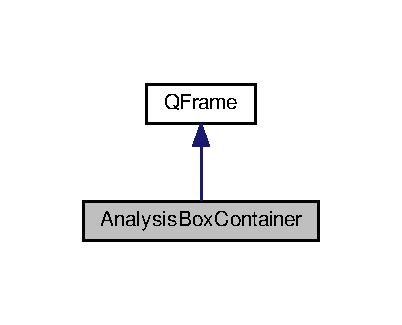
\includegraphics[width=193pt]{classGUI_1_1AnalysisBoxContainer__inherit__graph}
\end{center}
\end{figure}
\subsection*{Public Member Functions}
\begin{DoxyCompactItemize}
\item 
\hyperlink{classGUI_1_1AnalysisBoxContainer_ae603e523cc42100eccf571ff85ca39e8}{Analysis\+Box\+Container} (\hyperlink{classGUI_1_1QWidget}{G\+U\+I\+::\+Q\+Widget} $\ast$parent)
\item 
\hyperlink{classMemento_1_1AnalysisBoxContainerMemento}{Memento\+::\+Analysis\+Box\+Container\+Memento} \hyperlink{classGUI_1_1AnalysisBoxContainer_a0743a7c422123fbd5d22a946af5092ca}{get\+Memento} ()
\item 
void \hyperlink{classGUI_1_1AnalysisBoxContainer_af6d8c35bc3f7000da0579310af42e756}{restore} (\hyperlink{classMemento_1_1AnalysisBoxContainerMemento}{Memento\+::\+Analysis\+Box\+Container\+Memento} memento)
\item 
void \hyperlink{classGUI_1_1AnalysisBoxContainer_af3b761e148d9cb7352c5ffb4bf4c66bd}{add\+Video} (Q\+String path)
\item 
void \hyperlink{classGUI_1_1AnalysisBoxContainer_aa08759618dc05b98d60dc8942d41b556}{set\+Raw\+Video} (\hyperlink{classGUI_1_1Video}{G\+U\+I\+::\+Video} $\ast$video)
\item 
void \hyperlink{classGUI_1_1AnalysisBoxContainer_a678bedcbfc074efd29b5587a753fc341}{set\+Timer} (shared\+\_\+ptr$<$ \hyperlink{classGUI_1_1Timer}{G\+U\+I\+::\+Timer} $>$ timer\+:std\+:)
\item 
void \hyperlink{classGUI_1_1AnalysisBoxContainer_a9c1b482d1dcd6a733b84a9cdcc960263}{set\+Control\+Panel} (Player\+::\+Global\+Control\+Panel $\ast$panel)
\item 
void \hyperlink{classGUI_1_1AnalysisBoxContainer_ab3d9dc42d8e78c5bf6f87c5e93bdf1ce}{show\+Macro\+Block\+Videos} ()
\item 
void \hyperlink{classGUI_1_1AnalysisBoxContainer_a91638333a4b3fe577fd2062f2aa667f3}{show\+R\+G\+B\+Difference\+Videos} ()
\item 
void \hyperlink{classGUI_1_1AnalysisBoxContainer_a181a2114e38722fcae5a9c1d5b1d0ff7}{remove\+Box} (\hyperlink{classGUI_1_1AnalysisBox}{G\+U\+I\+::\+Analysis\+Box} \&box)
\item 
\hyperlink{classGUI_1_1AnalysisBox}{G\+U\+I\+::\+Analysis\+Box} $\ast$ \hyperlink{classGUI_1_1AnalysisBoxContainer_a483776769a5f7b2913128aa76251026b}{add\+Video} (\hyperlink{classModel_1_1EncodedVideo}{Model\+::\+Encoded\+Video} video)
\end{DoxyCompactItemize}
\subsection*{Data Fields}
\begin{DoxyCompactItemize}
\item 
\hyperlink{classUndoRedo_1_1RemoveVideo}{Undo\+Redo\+::\+Remove\+Video} $\ast$ \hyperlink{classGUI_1_1AnalysisBoxContainer_a14b06011d2f6be0da89f067a1e838b09}{ana\+Box\+Container}
\end{DoxyCompactItemize}
\subsection*{Private Attributes}
\begin{DoxyCompactItemize}
\item 
\hyperlink{classGUI_1_1Video}{G\+U\+I\+::\+Video} $\ast$ \hyperlink{classGUI_1_1AnalysisBoxContainer_a36ae288eba0c53b885d93498c8c68469}{raw\+Video}
\item 
shared\+\_\+ptr$<$ \hyperlink{classGUI_1_1Timer}{G\+U\+I\+::\+Timer} $>$ \hyperlink{classGUI_1_1AnalysisBoxContainer_a38f007cbe577c8cecfadf2358a3049fc}{timer}\+:std\+:
\item 
Player\+::\+Global\+Control\+Panel $\ast$ \hyperlink{classGUI_1_1AnalysisBoxContainer_aa7d83e3ba62ee643206acd2a48e058e3}{control\+Panel}
\item 
\hyperlink{classGUI_1_1AnalysisTab}{G\+U\+I\+::\+Analysis\+Tab} $\ast$ \hyperlink{classGUI_1_1AnalysisBoxContainer_a6754830af7090fa0a2bf7c94fbb188cc}{analysis\+Box\+Container}
\item 
std\+::vector$<$ \hyperlink{classGUI_1_1AnalysisBox}{G\+U\+I\+::\+Analysis\+Box} $\ast$ $>$ \hyperlink{classGUI_1_1AnalysisBoxContainer_a5083484e3ec5273e8a150e11fea5108b}{boxes}
\end{DoxyCompactItemize}


\subsection{Detailed Description}
Contains and manages the Analysis\+Boxes. 

\subsection{Constructor \& Destructor Documentation}
\hypertarget{classGUI_1_1AnalysisBoxContainer_ae603e523cc42100eccf571ff85ca39e8}{}\index{G\+U\+I\+::\+Analysis\+Box\+Container@{G\+U\+I\+::\+Analysis\+Box\+Container}!Analysis\+Box\+Container@{Analysis\+Box\+Container}}
\index{Analysis\+Box\+Container@{Analysis\+Box\+Container}!G\+U\+I\+::\+Analysis\+Box\+Container@{G\+U\+I\+::\+Analysis\+Box\+Container}}
\subsubsection[{Analysis\+Box\+Container}]{\setlength{\rightskip}{0pt plus 5cm}{\bf Analysis\+Box\+Container} (
\begin{DoxyParamCaption}
\item[{{\bf G\+U\+I\+::\+Q\+Widget} $\ast$}]{parent}
\end{DoxyParamCaption}
)}\label{classGUI_1_1AnalysisBoxContainer_ae603e523cc42100eccf571ff85ca39e8}


Constructor. 



\subsection{Member Function Documentation}
\hypertarget{classGUI_1_1AnalysisBoxContainer_af3b761e148d9cb7352c5ffb4bf4c66bd}{}\index{G\+U\+I\+::\+Analysis\+Box\+Container@{G\+U\+I\+::\+Analysis\+Box\+Container}!add\+Video@{add\+Video}}
\index{add\+Video@{add\+Video}!G\+U\+I\+::\+Analysis\+Box\+Container@{G\+U\+I\+::\+Analysis\+Box\+Container}}
\subsubsection[{add\+Video}]{\setlength{\rightskip}{0pt plus 5cm}void add\+Video (
\begin{DoxyParamCaption}
\item[{Q\+String}]{path}
\end{DoxyParamCaption}
)}\label{classGUI_1_1AnalysisBoxContainer_af3b761e148d9cb7352c5ffb4bf4c66bd}


Creates a Analysis box and shows it. 


\begin{DoxyParams}{Parameters}
{\em path} & The path of the video to analyse.\\
\hline
\end{DoxyParams}
\hypertarget{classGUI_1_1AnalysisBoxContainer_a483776769a5f7b2913128aa76251026b}{}\index{G\+U\+I\+::\+Analysis\+Box\+Container@{G\+U\+I\+::\+Analysis\+Box\+Container}!add\+Video@{add\+Video}}
\index{add\+Video@{add\+Video}!G\+U\+I\+::\+Analysis\+Box\+Container@{G\+U\+I\+::\+Analysis\+Box\+Container}}
\subsubsection[{add\+Video}]{\setlength{\rightskip}{0pt plus 5cm}{\bf G\+U\+I\+::\+Analysis\+Box}$\ast$ add\+Video (
\begin{DoxyParamCaption}
\item[{{\bf Model\+::\+Encoded\+Video}}]{video}
\end{DoxyParamCaption}
)}\label{classGUI_1_1AnalysisBoxContainer_a483776769a5f7b2913128aa76251026b}


Adds the given video to the container. 


\begin{DoxyParams}{Parameters}
{\em video} & The video to add.\\
\hline
\end{DoxyParams}
\begin{DoxyReturn}{Returns}
The box in which the video is presented.
\end{DoxyReturn}
\hypertarget{classGUI_1_1AnalysisBoxContainer_a0743a7c422123fbd5d22a946af5092ca}{}\index{G\+U\+I\+::\+Analysis\+Box\+Container@{G\+U\+I\+::\+Analysis\+Box\+Container}!get\+Memento@{get\+Memento}}
\index{get\+Memento@{get\+Memento}!G\+U\+I\+::\+Analysis\+Box\+Container@{G\+U\+I\+::\+Analysis\+Box\+Container}}
\subsubsection[{get\+Memento}]{\setlength{\rightskip}{0pt plus 5cm}{\bf Memento\+::\+Analysis\+Box\+Container\+Memento} get\+Memento (
\begin{DoxyParamCaption}
{}
\end{DoxyParamCaption}
)}\label{classGUI_1_1AnalysisBoxContainer_a0743a7c422123fbd5d22a946af5092ca}


Creates a memento which contains the state of the container. 

\begin{DoxyReturn}{Returns}
The created memento.
\end{DoxyReturn}
\hypertarget{classGUI_1_1AnalysisBoxContainer_a181a2114e38722fcae5a9c1d5b1d0ff7}{}\index{G\+U\+I\+::\+Analysis\+Box\+Container@{G\+U\+I\+::\+Analysis\+Box\+Container}!remove\+Box@{remove\+Box}}
\index{remove\+Box@{remove\+Box}!G\+U\+I\+::\+Analysis\+Box\+Container@{G\+U\+I\+::\+Analysis\+Box\+Container}}
\subsubsection[{remove\+Box}]{\setlength{\rightskip}{0pt plus 5cm}void remove\+Box (
\begin{DoxyParamCaption}
\item[{{\bf G\+U\+I\+::\+Analysis\+Box} \&}]{box}
\end{DoxyParamCaption}
)}\label{classGUI_1_1AnalysisBoxContainer_a181a2114e38722fcae5a9c1d5b1d0ff7}


Removes a box from the list. 


\begin{DoxyParams}{Parameters}
{\em box} & The box to remove.\\
\hline
\end{DoxyParams}
\hypertarget{classGUI_1_1AnalysisBoxContainer_af6d8c35bc3f7000da0579310af42e756}{}\index{G\+U\+I\+::\+Analysis\+Box\+Container@{G\+U\+I\+::\+Analysis\+Box\+Container}!restore@{restore}}
\index{restore@{restore}!G\+U\+I\+::\+Analysis\+Box\+Container@{G\+U\+I\+::\+Analysis\+Box\+Container}}
\subsubsection[{restore}]{\setlength{\rightskip}{0pt plus 5cm}void restore (
\begin{DoxyParamCaption}
\item[{{\bf Memento\+::\+Analysis\+Box\+Container\+Memento}}]{memento}
\end{DoxyParamCaption}
)}\label{classGUI_1_1AnalysisBoxContainer_af6d8c35bc3f7000da0579310af42e756}


Restores the container based on the memento. 


\begin{DoxyParams}{Parameters}
{\em memento} & The memento which contains the state to restore.\\
\hline
\end{DoxyParams}
\hypertarget{classGUI_1_1AnalysisBoxContainer_a9c1b482d1dcd6a733b84a9cdcc960263}{}\index{G\+U\+I\+::\+Analysis\+Box\+Container@{G\+U\+I\+::\+Analysis\+Box\+Container}!set\+Control\+Panel@{set\+Control\+Panel}}
\index{set\+Control\+Panel@{set\+Control\+Panel}!G\+U\+I\+::\+Analysis\+Box\+Container@{G\+U\+I\+::\+Analysis\+Box\+Container}}
\subsubsection[{set\+Control\+Panel}]{\setlength{\rightskip}{0pt plus 5cm}void set\+Control\+Panel (
\begin{DoxyParamCaption}
\item[{Player\+::\+Global\+Control\+Panel $\ast$}]{panel}
\end{DoxyParamCaption}
)}\label{classGUI_1_1AnalysisBoxContainer_a9c1b482d1dcd6a733b84a9cdcc960263}


Sets the \hyperlink{classGUI_1_1GlobalControlPanel}{Global\+Control\+Panel}. 


\begin{DoxyParams}{Parameters}
{\em panel} & The panel.\\
\hline
\end{DoxyParams}
\hypertarget{classGUI_1_1AnalysisBoxContainer_aa08759618dc05b98d60dc8942d41b556}{}\index{G\+U\+I\+::\+Analysis\+Box\+Container@{G\+U\+I\+::\+Analysis\+Box\+Container}!set\+Raw\+Video@{set\+Raw\+Video}}
\index{set\+Raw\+Video@{set\+Raw\+Video}!G\+U\+I\+::\+Analysis\+Box\+Container@{G\+U\+I\+::\+Analysis\+Box\+Container}}
\subsubsection[{set\+Raw\+Video}]{\setlength{\rightskip}{0pt plus 5cm}void set\+Raw\+Video (
\begin{DoxyParamCaption}
\item[{{\bf G\+U\+I\+::\+Video} $\ast$}]{video}
\end{DoxyParamCaption}
)}\label{classGUI_1_1AnalysisBoxContainer_aa08759618dc05b98d60dc8942d41b556}


Sets the raw\+Video the encoded videos are compared to. 


\begin{DoxyParams}{Parameters}
{\em video} & The raw video.\\
\hline
\end{DoxyParams}
\hypertarget{classGUI_1_1AnalysisBoxContainer_a678bedcbfc074efd29b5587a753fc341}{}\index{G\+U\+I\+::\+Analysis\+Box\+Container@{G\+U\+I\+::\+Analysis\+Box\+Container}!set\+Timer@{set\+Timer}}
\index{set\+Timer@{set\+Timer}!G\+U\+I\+::\+Analysis\+Box\+Container@{G\+U\+I\+::\+Analysis\+Box\+Container}}
\subsubsection[{set\+Timer}]{\setlength{\rightskip}{0pt plus 5cm}void set\+Timer (
\begin{DoxyParamCaption}
\item[{shared\+\_\+ptr$<$ {\bf G\+U\+I\+::\+Timer} $>$ timer\+:std\+:}]{}
\end{DoxyParamCaption}
)}\label{classGUI_1_1AnalysisBoxContainer_a678bedcbfc074efd29b5587a753fc341}


Sets the timer for the videoplayers. 


\begin{DoxyParams}{Parameters}
{\em timer\+:std,\+:} & The timer for the videoplayers.\\
\hline
\end{DoxyParams}
\hypertarget{classGUI_1_1AnalysisBoxContainer_ab3d9dc42d8e78c5bf6f87c5e93bdf1ce}{}\index{G\+U\+I\+::\+Analysis\+Box\+Container@{G\+U\+I\+::\+Analysis\+Box\+Container}!show\+Macro\+Block\+Videos@{show\+Macro\+Block\+Videos}}
\index{show\+Macro\+Block\+Videos@{show\+Macro\+Block\+Videos}!G\+U\+I\+::\+Analysis\+Box\+Container@{G\+U\+I\+::\+Analysis\+Box\+Container}}
\subsubsection[{show\+Macro\+Block\+Videos}]{\setlength{\rightskip}{0pt plus 5cm}void show\+Macro\+Block\+Videos (
\begin{DoxyParamCaption}
{}
\end{DoxyParamCaption}
)}\label{classGUI_1_1AnalysisBoxContainer_ab3d9dc42d8e78c5bf6f87c5e93bdf1ce}


Tells all Analysis\+Boxes to show the macro block video. 

\hypertarget{classGUI_1_1AnalysisBoxContainer_a91638333a4b3fe577fd2062f2aa667f3}{}\index{G\+U\+I\+::\+Analysis\+Box\+Container@{G\+U\+I\+::\+Analysis\+Box\+Container}!show\+R\+G\+B\+Difference\+Videos@{show\+R\+G\+B\+Difference\+Videos}}
\index{show\+R\+G\+B\+Difference\+Videos@{show\+R\+G\+B\+Difference\+Videos}!G\+U\+I\+::\+Analysis\+Box\+Container@{G\+U\+I\+::\+Analysis\+Box\+Container}}
\subsubsection[{show\+R\+G\+B\+Difference\+Videos}]{\setlength{\rightskip}{0pt plus 5cm}void show\+R\+G\+B\+Difference\+Videos (
\begin{DoxyParamCaption}
{}
\end{DoxyParamCaption}
)}\label{classGUI_1_1AnalysisBoxContainer_a91638333a4b3fe577fd2062f2aa667f3}


Tells all Analysis\+Boxes to show the R\+G\+B\+Diff video. 



\subsection{Field Documentation}
\hypertarget{classGUI_1_1AnalysisBoxContainer_a14b06011d2f6be0da89f067a1e838b09}{}\index{G\+U\+I\+::\+Analysis\+Box\+Container@{G\+U\+I\+::\+Analysis\+Box\+Container}!ana\+Box\+Container@{ana\+Box\+Container}}
\index{ana\+Box\+Container@{ana\+Box\+Container}!G\+U\+I\+::\+Analysis\+Box\+Container@{G\+U\+I\+::\+Analysis\+Box\+Container}}
\subsubsection[{ana\+Box\+Container}]{\setlength{\rightskip}{0pt plus 5cm}{\bf Undo\+Redo\+::\+Remove\+Video}$\ast$ ana\+Box\+Container}\label{classGUI_1_1AnalysisBoxContainer_a14b06011d2f6be0da89f067a1e838b09}
\hypertarget{classGUI_1_1AnalysisBoxContainer_a6754830af7090fa0a2bf7c94fbb188cc}{}\index{G\+U\+I\+::\+Analysis\+Box\+Container@{G\+U\+I\+::\+Analysis\+Box\+Container}!analysis\+Box\+Container@{analysis\+Box\+Container}}
\index{analysis\+Box\+Container@{analysis\+Box\+Container}!G\+U\+I\+::\+Analysis\+Box\+Container@{G\+U\+I\+::\+Analysis\+Box\+Container}}
\subsubsection[{analysis\+Box\+Container}]{\setlength{\rightskip}{0pt plus 5cm}{\bf G\+U\+I\+::\+Analysis\+Tab}$\ast$ analysis\+Box\+Container\hspace{0.3cm}{\ttfamily [private]}}\label{classGUI_1_1AnalysisBoxContainer_a6754830af7090fa0a2bf7c94fbb188cc}
\hypertarget{classGUI_1_1AnalysisBoxContainer_a5083484e3ec5273e8a150e11fea5108b}{}\index{G\+U\+I\+::\+Analysis\+Box\+Container@{G\+U\+I\+::\+Analysis\+Box\+Container}!boxes@{boxes}}
\index{boxes@{boxes}!G\+U\+I\+::\+Analysis\+Box\+Container@{G\+U\+I\+::\+Analysis\+Box\+Container}}
\subsubsection[{boxes}]{\setlength{\rightskip}{0pt plus 5cm}std\+::vector$<${\bf G\+U\+I\+::\+Analysis\+Box}$\ast$$>$ boxes\hspace{0.3cm}{\ttfamily [private]}}\label{classGUI_1_1AnalysisBoxContainer_a5083484e3ec5273e8a150e11fea5108b}
\hypertarget{classGUI_1_1AnalysisBoxContainer_aa7d83e3ba62ee643206acd2a48e058e3}{}\index{G\+U\+I\+::\+Analysis\+Box\+Container@{G\+U\+I\+::\+Analysis\+Box\+Container}!control\+Panel@{control\+Panel}}
\index{control\+Panel@{control\+Panel}!G\+U\+I\+::\+Analysis\+Box\+Container@{G\+U\+I\+::\+Analysis\+Box\+Container}}
\subsubsection[{control\+Panel}]{\setlength{\rightskip}{0pt plus 5cm}Player\+::\+Global\+Control\+Panel$\ast$ control\+Panel\hspace{0.3cm}{\ttfamily [private]}}\label{classGUI_1_1AnalysisBoxContainer_aa7d83e3ba62ee643206acd2a48e058e3}
\hypertarget{classGUI_1_1AnalysisBoxContainer_a36ae288eba0c53b885d93498c8c68469}{}\index{G\+U\+I\+::\+Analysis\+Box\+Container@{G\+U\+I\+::\+Analysis\+Box\+Container}!raw\+Video@{raw\+Video}}
\index{raw\+Video@{raw\+Video}!G\+U\+I\+::\+Analysis\+Box\+Container@{G\+U\+I\+::\+Analysis\+Box\+Container}}
\subsubsection[{raw\+Video}]{\setlength{\rightskip}{0pt plus 5cm}{\bf G\+U\+I\+::\+Video}$\ast$ raw\+Video\hspace{0.3cm}{\ttfamily [private]}}\label{classGUI_1_1AnalysisBoxContainer_a36ae288eba0c53b885d93498c8c68469}
\hypertarget{classGUI_1_1AnalysisBoxContainer_a38f007cbe577c8cecfadf2358a3049fc}{}\index{G\+U\+I\+::\+Analysis\+Box\+Container@{G\+U\+I\+::\+Analysis\+Box\+Container}!timer@{timer}}
\index{timer@{timer}!G\+U\+I\+::\+Analysis\+Box\+Container@{G\+U\+I\+::\+Analysis\+Box\+Container}}
\subsubsection[{timer}]{\setlength{\rightskip}{0pt plus 5cm}shared\+\_\+ptr$<${\bf G\+U\+I\+::\+Timer}$>$ timer\hspace{0.3cm}{\ttfamily [private]}}\label{classGUI_1_1AnalysisBoxContainer_a38f007cbe577c8cecfadf2358a3049fc}

\hypertarget{classMemento_1_1AnalysisBoxContainerMemento}{}\section{Analysis\+Box\+Container\+Memento Class Reference}
\label{classMemento_1_1AnalysisBoxContainerMemento}\index{Analysis\+Box\+Container\+Memento@{Analysis\+Box\+Container\+Memento}}
\subsection*{Public Member Functions}
\begin{DoxyCompactItemize}
\item 
void \hyperlink{classMemento_1_1AnalysisBoxContainerMemento_a93c3e248eed6b6359984e54bdc3a560d}{analyse\+Box\+Memento} ()
\item 
vector$<$ \hyperlink{classMemento_1_1AnalysisBoxMemento}{Memento\+::\+Analysis\+Box\+Memento} $>$ \hyperlink{classMemento_1_1AnalysisBoxContainerMemento_a8b5776381bcb34875736a6436e848112}{get\+Analysis\+Box\+List} ()
\item 
void \hyperlink{classMemento_1_1AnalysisBoxContainerMemento_a1584f5be1afbee957c6a9a33dc4a6317}{set\+Analysis\+Box\+List} (vector$<$ \hyperlink{classMemento_1_1AnalysisBoxMemento}{Memento\+::\+Analysis\+Box\+Memento} $>$ analyse\+Box\+List\+:std\+:)
\end{DoxyCompactItemize}


\subsection{Detailed Description}
This class is the memento for the Analysis\+Box\+Container. 

\subsection{Member Function Documentation}
\hypertarget{classMemento_1_1AnalysisBoxContainerMemento_a93c3e248eed6b6359984e54bdc3a560d}{}\index{Memento\+::\+Analysis\+Box\+Container\+Memento@{Memento\+::\+Analysis\+Box\+Container\+Memento}!analyse\+Box\+Memento@{analyse\+Box\+Memento}}
\index{analyse\+Box\+Memento@{analyse\+Box\+Memento}!Memento\+::\+Analysis\+Box\+Container\+Memento@{Memento\+::\+Analysis\+Box\+Container\+Memento}}
\subsubsection[{analyse\+Box\+Memento}]{\setlength{\rightskip}{0pt plus 5cm}void analyse\+Box\+Memento (
\begin{DoxyParamCaption}
{}
\end{DoxyParamCaption}
)}\label{classMemento_1_1AnalysisBoxContainerMemento_a93c3e248eed6b6359984e54bdc3a560d}


Constructor. 

\hypertarget{classMemento_1_1AnalysisBoxContainerMemento_a8b5776381bcb34875736a6436e848112}{}\index{Memento\+::\+Analysis\+Box\+Container\+Memento@{Memento\+::\+Analysis\+Box\+Container\+Memento}!get\+Analysis\+Box\+List@{get\+Analysis\+Box\+List}}
\index{get\+Analysis\+Box\+List@{get\+Analysis\+Box\+List}!Memento\+::\+Analysis\+Box\+Container\+Memento@{Memento\+::\+Analysis\+Box\+Container\+Memento}}
\subsubsection[{get\+Analysis\+Box\+List}]{\setlength{\rightskip}{0pt plus 5cm}vector$<$ {\bf Memento\+::\+Analysis\+Box\+Memento} $>$ get\+Analysis\+Box\+List (
\begin{DoxyParamCaption}
{}
\end{DoxyParamCaption}
)}\label{classMemento_1_1AnalysisBoxContainerMemento_a8b5776381bcb34875736a6436e848112}


Returns a list of Analysis\+Box mementos. 

\begin{DoxyReturn}{Returns}
a lists of \hyperlink{classMemento_1_1AnalysisBoxMemento}{Analysis\+Box\+Memento}
\end{DoxyReturn}
\hypertarget{classMemento_1_1AnalysisBoxContainerMemento_a1584f5be1afbee957c6a9a33dc4a6317}{}\index{Memento\+::\+Analysis\+Box\+Container\+Memento@{Memento\+::\+Analysis\+Box\+Container\+Memento}!set\+Analysis\+Box\+List@{set\+Analysis\+Box\+List}}
\index{set\+Analysis\+Box\+List@{set\+Analysis\+Box\+List}!Memento\+::\+Analysis\+Box\+Container\+Memento@{Memento\+::\+Analysis\+Box\+Container\+Memento}}
\subsubsection[{set\+Analysis\+Box\+List}]{\setlength{\rightskip}{0pt plus 5cm}void set\+Analysis\+Box\+List (
\begin{DoxyParamCaption}
\item[{vector$<$ {\bf Memento\+::\+Analysis\+Box\+Memento} $>$ analyse\+Box\+List\+:std\+:}]{}
\end{DoxyParamCaption}
)}\label{classMemento_1_1AnalysisBoxContainerMemento_a1584f5be1afbee957c6a9a33dc4a6317}


Sets the list of \hyperlink{classMemento_1_1AnalysisBoxMemento}{Analysis\+Box\+Memento} 


\begin{DoxyParams}{Parameters}
{\em analyse\+Box\+List\+:std,\+:} & the list of the mementos\\
\hline
\end{DoxyParams}

\hypertarget{classMemento_1_1AnalysisBoxMemento}{}\section{Analysis\+Box\+Memento Class Reference}
\label{classMemento_1_1AnalysisBoxMemento}\index{Analysis\+Box\+Memento@{Analysis\+Box\+Memento}}
\subsection*{Public Member Functions}
\begin{DoxyCompactItemize}
\item 
\hyperlink{classMemento_1_1AnalysisBoxMemento_a2891757dd897d8d7e04f6ac721863e30}{Analysis\+Box\+Memento} ()
\item 
Q\+String \hyperlink{classMemento_1_1AnalysisBoxMemento_a0aee21e65efbd5059679492dcb847281}{get\+Video\+Path} ()
\item 
void \hyperlink{classMemento_1_1AnalysisBoxMemento_a3db0ccff589bc23a3226a0ac59857437}{set\+Video\+Path} (Q\+String video\+Path)
\item 
Q\+String \hyperlink{classMemento_1_1AnalysisBoxMemento_a8475ee6c96bf1157aa07530f9100416c}{get\+Comment} ()
\item 
void \hyperlink{classMemento_1_1AnalysisBoxMemento_ab3a897eff60f58840c8d1b40292cf047}{set\+Comment} (Q\+String comment)
\item 
\hyperlink{classGUI_1_1Player_1_1Video}{G\+U\+I\+::\+Player\+::\+Video} $\ast$ \hyperlink{classMemento_1_1AnalysisBoxMemento_a4766ee11b86f10503824b3dc18ec3a6d}{get\+Macro\+Video} ()
\item 
void \hyperlink{classMemento_1_1AnalysisBoxMemento_ab43a2220425e3311fa978cebe61db3e4}{set\+Macro\+Video} (\hyperlink{classGUI_1_1Player_1_1Video}{G\+U\+I\+::\+Player\+::\+Video} $\ast$macro\+Video)
\item 
\hyperlink{classGUI_1_1Player_1_1Video}{G\+U\+I\+::\+Player\+::\+Video} $\ast$ \hyperlink{classMemento_1_1AnalysisBoxMemento_aeafaf51d6b8da8f5015d7887cf00c474}{get\+Rgb\+Diff\+Video} ()
\item 
void \hyperlink{classMemento_1_1AnalysisBoxMemento_a15413d63ffb3c5f97f39d3c2f11b5c0e}{set\+Rgb\+Diff\+Video} (\hyperlink{classGUI_1_1Player_1_1Video}{G\+U\+I\+::\+Player\+::\+Video} $\ast$rgb\+Diff\+Video)
\item 
Q\+Image \hyperlink{classMemento_1_1AnalysisBoxMemento_a581aa3ebb51a9ce69dcbe21d6f949e99}{get\+Psnr} ()
\item 
void \hyperlink{classMemento_1_1AnalysisBoxMemento_a5613ac52b106bb5859856712c3a3279f}{set\+Psnr} (Q\+Image psnr)
\item 
Q\+Image \hyperlink{classMemento_1_1AnalysisBoxMemento_a0b8e4c45925b9a6f85c327561d7a4369}{get\+Bitrate} ()
\item 
void \hyperlink{classMemento_1_1AnalysisBoxMemento_ad755ae317fc096de20872b5daf21d69d}{set\+Bitrate} (Q\+Image bitrate)
\end{DoxyCompactItemize}


\subsection{Detailed Description}
This class is the memento for the Analysis\+Box. 

\subsection{Constructor \& Destructor Documentation}
\hypertarget{classMemento_1_1AnalysisBoxMemento_a2891757dd897d8d7e04f6ac721863e30}{}\index{Memento\+::\+Analysis\+Box\+Memento@{Memento\+::\+Analysis\+Box\+Memento}!Analysis\+Box\+Memento@{Analysis\+Box\+Memento}}
\index{Analysis\+Box\+Memento@{Analysis\+Box\+Memento}!Memento\+::\+Analysis\+Box\+Memento@{Memento\+::\+Analysis\+Box\+Memento}}
\subsubsection[{Analysis\+Box\+Memento}]{\setlength{\rightskip}{0pt plus 5cm}{\bf Analysis\+Box\+Memento} (
\begin{DoxyParamCaption}
{}
\end{DoxyParamCaption}
)}\label{classMemento_1_1AnalysisBoxMemento_a2891757dd897d8d7e04f6ac721863e30}


Constrictor. 



\subsection{Member Function Documentation}
\hypertarget{classMemento_1_1AnalysisBoxMemento_a0b8e4c45925b9a6f85c327561d7a4369}{}\index{Memento\+::\+Analysis\+Box\+Memento@{Memento\+::\+Analysis\+Box\+Memento}!get\+Bitrate@{get\+Bitrate}}
\index{get\+Bitrate@{get\+Bitrate}!Memento\+::\+Analysis\+Box\+Memento@{Memento\+::\+Analysis\+Box\+Memento}}
\subsubsection[{get\+Bitrate}]{\setlength{\rightskip}{0pt plus 5cm}Q\+Image get\+Bitrate (
\begin{DoxyParamCaption}
{}
\end{DoxyParamCaption}
)}\label{classMemento_1_1AnalysisBoxMemento_a0b8e4c45925b9a6f85c327561d7a4369}


Returns an image of the bitrate graph. 

\begin{DoxyReturn}{Returns}
an image of the bitrate graph
\end{DoxyReturn}
\hypertarget{classMemento_1_1AnalysisBoxMemento_a8475ee6c96bf1157aa07530f9100416c}{}\index{Memento\+::\+Analysis\+Box\+Memento@{Memento\+::\+Analysis\+Box\+Memento}!get\+Comment@{get\+Comment}}
\index{get\+Comment@{get\+Comment}!Memento\+::\+Analysis\+Box\+Memento@{Memento\+::\+Analysis\+Box\+Memento}}
\subsubsection[{get\+Comment}]{\setlength{\rightskip}{0pt plus 5cm}Q\+String get\+Comment (
\begin{DoxyParamCaption}
{}
\end{DoxyParamCaption}
)}\label{classMemento_1_1AnalysisBoxMemento_a8475ee6c96bf1157aa07530f9100416c}


Returns the user comment. 

\begin{DoxyReturn}{Returns}
the user comment
\end{DoxyReturn}
\hypertarget{classMemento_1_1AnalysisBoxMemento_a4766ee11b86f10503824b3dc18ec3a6d}{}\index{Memento\+::\+Analysis\+Box\+Memento@{Memento\+::\+Analysis\+Box\+Memento}!get\+Macro\+Video@{get\+Macro\+Video}}
\index{get\+Macro\+Video@{get\+Macro\+Video}!Memento\+::\+Analysis\+Box\+Memento@{Memento\+::\+Analysis\+Box\+Memento}}
\subsubsection[{get\+Macro\+Video}]{\setlength{\rightskip}{0pt plus 5cm}{\bf G\+U\+I\+::\+Player\+::\+Video} $\ast$ get\+Macro\+Video (
\begin{DoxyParamCaption}
{}
\end{DoxyParamCaption}
)}\label{classMemento_1_1AnalysisBoxMemento_a4766ee11b86f10503824b3dc18ec3a6d}


Returns the macroblock video. 

\begin{DoxyReturn}{Returns}
the macroblock video
\end{DoxyReturn}
\hypertarget{classMemento_1_1AnalysisBoxMemento_a581aa3ebb51a9ce69dcbe21d6f949e99}{}\index{Memento\+::\+Analysis\+Box\+Memento@{Memento\+::\+Analysis\+Box\+Memento}!get\+Psnr@{get\+Psnr}}
\index{get\+Psnr@{get\+Psnr}!Memento\+::\+Analysis\+Box\+Memento@{Memento\+::\+Analysis\+Box\+Memento}}
\subsubsection[{get\+Psnr}]{\setlength{\rightskip}{0pt plus 5cm}Q\+Image get\+Psnr (
\begin{DoxyParamCaption}
{}
\end{DoxyParamCaption}
)}\label{classMemento_1_1AnalysisBoxMemento_a581aa3ebb51a9ce69dcbe21d6f949e99}


Returns an image of the psnr graph. 

\begin{DoxyReturn}{Returns}
an image of the psnr graph
\end{DoxyReturn}
\hypertarget{classMemento_1_1AnalysisBoxMemento_aeafaf51d6b8da8f5015d7887cf00c474}{}\index{Memento\+::\+Analysis\+Box\+Memento@{Memento\+::\+Analysis\+Box\+Memento}!get\+Rgb\+Diff\+Video@{get\+Rgb\+Diff\+Video}}
\index{get\+Rgb\+Diff\+Video@{get\+Rgb\+Diff\+Video}!Memento\+::\+Analysis\+Box\+Memento@{Memento\+::\+Analysis\+Box\+Memento}}
\subsubsection[{get\+Rgb\+Diff\+Video}]{\setlength{\rightskip}{0pt plus 5cm}{\bf G\+U\+I\+::\+Player\+::\+Video} $\ast$ get\+Rgb\+Diff\+Video (
\begin{DoxyParamCaption}
{}
\end{DoxyParamCaption}
)}\label{classMemento_1_1AnalysisBoxMemento_aeafaf51d6b8da8f5015d7887cf00c474}


Returns the rgb difference video. 

\begin{DoxyReturn}{Returns}
the rgb difference video
\end{DoxyReturn}
\hypertarget{classMemento_1_1AnalysisBoxMemento_a0aee21e65efbd5059679492dcb847281}{}\index{Memento\+::\+Analysis\+Box\+Memento@{Memento\+::\+Analysis\+Box\+Memento}!get\+Video\+Path@{get\+Video\+Path}}
\index{get\+Video\+Path@{get\+Video\+Path}!Memento\+::\+Analysis\+Box\+Memento@{Memento\+::\+Analysis\+Box\+Memento}}
\subsubsection[{get\+Video\+Path}]{\setlength{\rightskip}{0pt plus 5cm}Q\+String get\+Video\+Path (
\begin{DoxyParamCaption}
{}
\end{DoxyParamCaption}
)}\label{classMemento_1_1AnalysisBoxMemento_a0aee21e65efbd5059679492dcb847281}


Returns the path to the video. 

\begin{DoxyReturn}{Returns}
absolute path to the video
\end{DoxyReturn}
\hypertarget{classMemento_1_1AnalysisBoxMemento_ad755ae317fc096de20872b5daf21d69d}{}\index{Memento\+::\+Analysis\+Box\+Memento@{Memento\+::\+Analysis\+Box\+Memento}!set\+Bitrate@{set\+Bitrate}}
\index{set\+Bitrate@{set\+Bitrate}!Memento\+::\+Analysis\+Box\+Memento@{Memento\+::\+Analysis\+Box\+Memento}}
\subsubsection[{set\+Bitrate}]{\setlength{\rightskip}{0pt plus 5cm}void set\+Bitrate (
\begin{DoxyParamCaption}
\item[{Q\+Image}]{bitrate}
\end{DoxyParamCaption}
)}\label{classMemento_1_1AnalysisBoxMemento_ad755ae317fc096de20872b5daf21d69d}


Sets the image for the bitrate graph. 


\begin{DoxyParams}{Parameters}
{\em bitrate} & the image of the bitrate gaph\\
\hline
\end{DoxyParams}
\hypertarget{classMemento_1_1AnalysisBoxMemento_ab3a897eff60f58840c8d1b40292cf047}{}\index{Memento\+::\+Analysis\+Box\+Memento@{Memento\+::\+Analysis\+Box\+Memento}!set\+Comment@{set\+Comment}}
\index{set\+Comment@{set\+Comment}!Memento\+::\+Analysis\+Box\+Memento@{Memento\+::\+Analysis\+Box\+Memento}}
\subsubsection[{set\+Comment}]{\setlength{\rightskip}{0pt plus 5cm}void set\+Comment (
\begin{DoxyParamCaption}
\item[{Q\+String}]{comment}
\end{DoxyParamCaption}
)}\label{classMemento_1_1AnalysisBoxMemento_ab3a897eff60f58840c8d1b40292cf047}


Sets the user comment. 


\begin{DoxyParams}{Parameters}
{\em comment} & the user comment\\
\hline
\end{DoxyParams}
\hypertarget{classMemento_1_1AnalysisBoxMemento_ab43a2220425e3311fa978cebe61db3e4}{}\index{Memento\+::\+Analysis\+Box\+Memento@{Memento\+::\+Analysis\+Box\+Memento}!set\+Macro\+Video@{set\+Macro\+Video}}
\index{set\+Macro\+Video@{set\+Macro\+Video}!Memento\+::\+Analysis\+Box\+Memento@{Memento\+::\+Analysis\+Box\+Memento}}
\subsubsection[{set\+Macro\+Video}]{\setlength{\rightskip}{0pt plus 5cm}void set\+Macro\+Video (
\begin{DoxyParamCaption}
\item[{{\bf G\+U\+I\+::\+Player\+::\+Video} $\ast$}]{macro\+Video}
\end{DoxyParamCaption}
)}\label{classMemento_1_1AnalysisBoxMemento_ab43a2220425e3311fa978cebe61db3e4}


Sets the macroblock video. 


\begin{DoxyParams}{Parameters}
{\em macro\+Video} & the macroblock video\\
\hline
\end{DoxyParams}
\hypertarget{classMemento_1_1AnalysisBoxMemento_a5613ac52b106bb5859856712c3a3279f}{}\index{Memento\+::\+Analysis\+Box\+Memento@{Memento\+::\+Analysis\+Box\+Memento}!set\+Psnr@{set\+Psnr}}
\index{set\+Psnr@{set\+Psnr}!Memento\+::\+Analysis\+Box\+Memento@{Memento\+::\+Analysis\+Box\+Memento}}
\subsubsection[{set\+Psnr}]{\setlength{\rightskip}{0pt plus 5cm}void set\+Psnr (
\begin{DoxyParamCaption}
\item[{Q\+Image}]{psnr}
\end{DoxyParamCaption}
)}\label{classMemento_1_1AnalysisBoxMemento_a5613ac52b106bb5859856712c3a3279f}


Sets the image of the psnr graph. 


\begin{DoxyParams}{Parameters}
{\em psnr} & the image of the psnr graph\\
\hline
\end{DoxyParams}
\hypertarget{classMemento_1_1AnalysisBoxMemento_a15413d63ffb3c5f97f39d3c2f11b5c0e}{}\index{Memento\+::\+Analysis\+Box\+Memento@{Memento\+::\+Analysis\+Box\+Memento}!set\+Rgb\+Diff\+Video@{set\+Rgb\+Diff\+Video}}
\index{set\+Rgb\+Diff\+Video@{set\+Rgb\+Diff\+Video}!Memento\+::\+Analysis\+Box\+Memento@{Memento\+::\+Analysis\+Box\+Memento}}
\subsubsection[{set\+Rgb\+Diff\+Video}]{\setlength{\rightskip}{0pt plus 5cm}void set\+Rgb\+Diff\+Video (
\begin{DoxyParamCaption}
\item[{{\bf G\+U\+I\+::\+Player\+::\+Video} $\ast$}]{rgb\+Diff\+Video}
\end{DoxyParamCaption}
)}\label{classMemento_1_1AnalysisBoxMemento_a15413d63ffb3c5f97f39d3c2f11b5c0e}


Sets the rgb difference video. 


\begin{DoxyParams}{Parameters}
{\em rgb\+Diff\+Video} & the rgb difference video\\
\hline
\end{DoxyParams}
\hypertarget{classMemento_1_1AnalysisBoxMemento_a3db0ccff589bc23a3226a0ac59857437}{}\index{Memento\+::\+Analysis\+Box\+Memento@{Memento\+::\+Analysis\+Box\+Memento}!set\+Video\+Path@{set\+Video\+Path}}
\index{set\+Video\+Path@{set\+Video\+Path}!Memento\+::\+Analysis\+Box\+Memento@{Memento\+::\+Analysis\+Box\+Memento}}
\subsubsection[{set\+Video\+Path}]{\setlength{\rightskip}{0pt plus 5cm}void set\+Video\+Path (
\begin{DoxyParamCaption}
\item[{Q\+String}]{video\+Path}
\end{DoxyParamCaption}
)}\label{classMemento_1_1AnalysisBoxMemento_a3db0ccff589bc23a3226a0ac59857437}


Sets the path to the video. 


\begin{DoxyParams}{Parameters}
{\em video\+Path} & absolute path to the video\\
\hline
\end{DoxyParams}

\hypertarget{classGUI_1_1AnalysisTab}{}\section{Analysis\+Tab Class Reference}
\label{classGUI_1_1AnalysisTab}\index{Analysis\+Tab@{Analysis\+Tab}}
\subsection*{Public Member Functions}
\begin{DoxyCompactItemize}
\item 
\hypertarget{classGUI_1_1AnalysisTab_a544106f19b9119dd044e0b351af6b8a0}{}{\bfseries Analysis\+Tab} (\hyperlink{classGUI_1_1QtGui_1_1QWidget____10}{G\+U\+I\+::\+Qt\+Gui\+::\+Q\+Widget\+\_\+\+\_\+10} $\ast$parent)\label{classGUI_1_1AnalysisTab_a544106f19b9119dd044e0b351af6b8a0}

\item 
\hypertarget{classGUI_1_1AnalysisTab_ad452524ed628a2eba1f167f79469b829}{}\hyperlink{classMemento_1_1AnalysisTabMemento}{Memento\+::\+Analysis\+Tab\+Memento} {\bfseries get\+Memento} ()\label{classGUI_1_1AnalysisTab_ad452524ed628a2eba1f167f79469b829}

\item 
\hypertarget{classGUI_1_1AnalysisTab_a37a387e0b6f67a340ff7e60b2f8f7f24}{}void {\bfseries restore} (\hyperlink{classMemento_1_1AnalysisTabMemento}{Memento\+::\+Analysis\+Tab\+Memento} memento)\label{classGUI_1_1AnalysisTab_a37a387e0b6f67a340ff7e60b2f8f7f24}

\end{DoxyCompactItemize}
\subsection*{Data Fields}
\begin{DoxyCompactItemize}
\item 
\hypertarget{classGUI_1_1AnalysisTab_ad1a5ead95d905d9ec387ee6c95665c38}{}\hyperlink{classGUI_1_1Player_1_1FrameView}{G\+U\+I\+::\+Player\+::\+Frame\+View} $\ast$ {\bfseries raw\+Video\+View}\label{classGUI_1_1AnalysisTab_ad1a5ead95d905d9ec387ee6c95665c38}

\end{DoxyCompactItemize}


\subsection{Detailed Description}
the tab that shows videos and analyses them 
\hypertarget{classMemento_1_1AnalysisTabMemento}{}\section{Analysis\+Tab\+Memento Class Reference}
\label{classMemento_1_1AnalysisTabMemento}\index{Analysis\+Tab\+Memento@{Analysis\+Tab\+Memento}}
\subsection*{Public Member Functions}
\begin{DoxyCompactItemize}
\item 
\hyperlink{classMemento_1_1AnalysisTabMemento_a035f84d6066cdb7d8a475da4710d2e67}{Analysis\+Tab\+Memento} ()
\item 
int \hyperlink{classMemento_1_1AnalysisTabMemento_af7babc742dcea9250c73c408b2cfacf2}{get\+Current\+Video\+Position} ()
\item 
void \hyperlink{classMemento_1_1AnalysisTabMemento_a66ff926aa567b15381b5906cd65c6b7d}{set\+Current\+Video\+Position} (int current\+Video\+Position)
\item 
int \hyperlink{classMemento_1_1AnalysisTabMemento_a687a0fc92408cf713058eaf23abc22f3}{get\+Currently\+Shown\+Analysis\+Video} ()
\item 
void \hyperlink{classMemento_1_1AnalysisTabMemento_a1d76537f6e47c09e47bf15eefd26feff}{set\+Currently\+Shown\+Analysis\+Video} (int currently\+Shown\+Analysis\+Video)
\item 
float \hyperlink{classMemento_1_1AnalysisTabMemento_a4c7df241ee5989199664bfc3b336d228}{get\+Current\+Speed} ()
\item 
void \hyperlink{classMemento_1_1AnalysisTabMemento_aa99f3e18fe8363d1333c1ddedfa12084}{set\+Current\+Speed} (float current\+Speed)
\item 
\hyperlink{classMemento_1_1AnalysisBoxContainerMemento}{Memento\+::\+Analysis\+Box\+Container\+Memento} \hyperlink{classMemento_1_1AnalysisTabMemento_a1882d53a845bc483ee4974f633026043}{get\+Analysis\+Box\+Container\+Memento} ()
\item 
void \hyperlink{classMemento_1_1AnalysisTabMemento_aca56db151b2ff66e743215ac8bc5b942}{set\+Analysis\+Box\+Container\+Memento} (\hyperlink{classMemento_1_1AnalysisBoxContainerMemento}{Memento\+::\+Analysis\+Box\+Container\+Memento} analysis\+Box\+Container\+Memento)
\end{DoxyCompactItemize}


\subsection{Detailed Description}
This class is the memento for the analysis tab. 

\subsection{Constructor \& Destructor Documentation}
\hypertarget{classMemento_1_1AnalysisTabMemento_a035f84d6066cdb7d8a475da4710d2e67}{}\index{Memento\+::\+Analysis\+Tab\+Memento@{Memento\+::\+Analysis\+Tab\+Memento}!Analysis\+Tab\+Memento@{Analysis\+Tab\+Memento}}
\index{Analysis\+Tab\+Memento@{Analysis\+Tab\+Memento}!Memento\+::\+Analysis\+Tab\+Memento@{Memento\+::\+Analysis\+Tab\+Memento}}
\subsubsection[{Analysis\+Tab\+Memento}]{\setlength{\rightskip}{0pt plus 5cm}{\bf Analysis\+Tab\+Memento} (
\begin{DoxyParamCaption}
{}
\end{DoxyParamCaption}
)}\label{classMemento_1_1AnalysisTabMemento_a035f84d6066cdb7d8a475da4710d2e67}


Constructor. 



\subsection{Member Function Documentation}
\hypertarget{classMemento_1_1AnalysisTabMemento_a1882d53a845bc483ee4974f633026043}{}\index{Memento\+::\+Analysis\+Tab\+Memento@{Memento\+::\+Analysis\+Tab\+Memento}!get\+Analysis\+Box\+Container\+Memento@{get\+Analysis\+Box\+Container\+Memento}}
\index{get\+Analysis\+Box\+Container\+Memento@{get\+Analysis\+Box\+Container\+Memento}!Memento\+::\+Analysis\+Tab\+Memento@{Memento\+::\+Analysis\+Tab\+Memento}}
\subsubsection[{get\+Analysis\+Box\+Container\+Memento}]{\setlength{\rightskip}{0pt plus 5cm}{\bf Memento\+::\+Analysis\+Box\+Container\+Memento} get\+Analysis\+Box\+Container\+Memento (
\begin{DoxyParamCaption}
{}
\end{DoxyParamCaption}
)}\label{classMemento_1_1AnalysisTabMemento_a1882d53a845bc483ee4974f633026043}


Returns the memento of the Analysis\+Box\+Container. 

\begin{DoxyReturn}{Returns}
the memento of the Analysis\+Box\+Container
\end{DoxyReturn}
\hypertarget{classMemento_1_1AnalysisTabMemento_a687a0fc92408cf713058eaf23abc22f3}{}\index{Memento\+::\+Analysis\+Tab\+Memento@{Memento\+::\+Analysis\+Tab\+Memento}!get\+Currently\+Shown\+Analysis\+Video@{get\+Currently\+Shown\+Analysis\+Video}}
\index{get\+Currently\+Shown\+Analysis\+Video@{get\+Currently\+Shown\+Analysis\+Video}!Memento\+::\+Analysis\+Tab\+Memento@{Memento\+::\+Analysis\+Tab\+Memento}}
\subsubsection[{get\+Currently\+Shown\+Analysis\+Video}]{\setlength{\rightskip}{0pt plus 5cm}int get\+Currently\+Shown\+Analysis\+Video (
\begin{DoxyParamCaption}
{}
\end{DoxyParamCaption}
)}\label{classMemento_1_1AnalysisTabMemento_a687a0fc92408cf713058eaf23abc22f3}


Returns what analysis video is currently shown. 0 means rgb difference. non zero means macroblocks. 

\begin{DoxyReturn}{Returns}
the currently shown analysis video
\end{DoxyReturn}
\hypertarget{classMemento_1_1AnalysisTabMemento_a4c7df241ee5989199664bfc3b336d228}{}\index{Memento\+::\+Analysis\+Tab\+Memento@{Memento\+::\+Analysis\+Tab\+Memento}!get\+Current\+Speed@{get\+Current\+Speed}}
\index{get\+Current\+Speed@{get\+Current\+Speed}!Memento\+::\+Analysis\+Tab\+Memento@{Memento\+::\+Analysis\+Tab\+Memento}}
\subsubsection[{get\+Current\+Speed}]{\setlength{\rightskip}{0pt plus 5cm}float get\+Current\+Speed (
\begin{DoxyParamCaption}
{}
\end{DoxyParamCaption}
)}\label{classMemento_1_1AnalysisTabMemento_a4c7df241ee5989199664bfc3b336d228}


Returns the current speed of the player. 

\begin{DoxyReturn}{Returns}
the current speed of the player
\end{DoxyReturn}
\hypertarget{classMemento_1_1AnalysisTabMemento_af7babc742dcea9250c73c408b2cfacf2}{}\index{Memento\+::\+Analysis\+Tab\+Memento@{Memento\+::\+Analysis\+Tab\+Memento}!get\+Current\+Video\+Position@{get\+Current\+Video\+Position}}
\index{get\+Current\+Video\+Position@{get\+Current\+Video\+Position}!Memento\+::\+Analysis\+Tab\+Memento@{Memento\+::\+Analysis\+Tab\+Memento}}
\subsubsection[{get\+Current\+Video\+Position}]{\setlength{\rightskip}{0pt plus 5cm}int get\+Current\+Video\+Position (
\begin{DoxyParamCaption}
{}
\end{DoxyParamCaption}
)}\label{classMemento_1_1AnalysisTabMemento_af7babc742dcea9250c73c408b2cfacf2}


Returns the current position the player is at. 

\begin{DoxyReturn}{Returns}
the current position of the player
\end{DoxyReturn}
\hypertarget{classMemento_1_1AnalysisTabMemento_aca56db151b2ff66e743215ac8bc5b942}{}\index{Memento\+::\+Analysis\+Tab\+Memento@{Memento\+::\+Analysis\+Tab\+Memento}!set\+Analysis\+Box\+Container\+Memento@{set\+Analysis\+Box\+Container\+Memento}}
\index{set\+Analysis\+Box\+Container\+Memento@{set\+Analysis\+Box\+Container\+Memento}!Memento\+::\+Analysis\+Tab\+Memento@{Memento\+::\+Analysis\+Tab\+Memento}}
\subsubsection[{set\+Analysis\+Box\+Container\+Memento}]{\setlength{\rightskip}{0pt plus 5cm}void set\+Analysis\+Box\+Container\+Memento (
\begin{DoxyParamCaption}
\item[{{\bf Memento\+::\+Analysis\+Box\+Container\+Memento}}]{analysis\+Box\+Container\+Memento}
\end{DoxyParamCaption}
)}\label{classMemento_1_1AnalysisTabMemento_aca56db151b2ff66e743215ac8bc5b942}


Sets the memento of the Analysis\+Box\+Container. 


\begin{DoxyParams}{Parameters}
{\em analysis\+Box\+Container\+Memento} & the memento of the Analysis\+Box\+Container\\
\hline
\end{DoxyParams}
\hypertarget{classMemento_1_1AnalysisTabMemento_a1d76537f6e47c09e47bf15eefd26feff}{}\index{Memento\+::\+Analysis\+Tab\+Memento@{Memento\+::\+Analysis\+Tab\+Memento}!set\+Currently\+Shown\+Analysis\+Video@{set\+Currently\+Shown\+Analysis\+Video}}
\index{set\+Currently\+Shown\+Analysis\+Video@{set\+Currently\+Shown\+Analysis\+Video}!Memento\+::\+Analysis\+Tab\+Memento@{Memento\+::\+Analysis\+Tab\+Memento}}
\subsubsection[{set\+Currently\+Shown\+Analysis\+Video}]{\setlength{\rightskip}{0pt plus 5cm}void set\+Currently\+Shown\+Analysis\+Video (
\begin{DoxyParamCaption}
\item[{int}]{currently\+Shown\+Analysis\+Video}
\end{DoxyParamCaption}
)}\label{classMemento_1_1AnalysisTabMemento_a1d76537f6e47c09e47bf15eefd26feff}


Sets the currently shown analysis video. 0 means rgb difference. non 0 means macroblocks. 


\begin{DoxyParams}{Parameters}
{\em currently\+Shown\+Analysis\+Video} & the currrently shown analysis video\\
\hline
\end{DoxyParams}
\hypertarget{classMemento_1_1AnalysisTabMemento_aa99f3e18fe8363d1333c1ddedfa12084}{}\index{Memento\+::\+Analysis\+Tab\+Memento@{Memento\+::\+Analysis\+Tab\+Memento}!set\+Current\+Speed@{set\+Current\+Speed}}
\index{set\+Current\+Speed@{set\+Current\+Speed}!Memento\+::\+Analysis\+Tab\+Memento@{Memento\+::\+Analysis\+Tab\+Memento}}
\subsubsection[{set\+Current\+Speed}]{\setlength{\rightskip}{0pt plus 5cm}void set\+Current\+Speed (
\begin{DoxyParamCaption}
\item[{float}]{current\+Speed}
\end{DoxyParamCaption}
)}\label{classMemento_1_1AnalysisTabMemento_aa99f3e18fe8363d1333c1ddedfa12084}


Sets the current speed of the player. 


\begin{DoxyParams}{Parameters}
{\em current\+Speed} & the current speed of the player\\
\hline
\end{DoxyParams}
\hypertarget{classMemento_1_1AnalysisTabMemento_a66ff926aa567b15381b5906cd65c6b7d}{}\index{Memento\+::\+Analysis\+Tab\+Memento@{Memento\+::\+Analysis\+Tab\+Memento}!set\+Current\+Video\+Position@{set\+Current\+Video\+Position}}
\index{set\+Current\+Video\+Position@{set\+Current\+Video\+Position}!Memento\+::\+Analysis\+Tab\+Memento@{Memento\+::\+Analysis\+Tab\+Memento}}
\subsubsection[{set\+Current\+Video\+Position}]{\setlength{\rightskip}{0pt plus 5cm}void set\+Current\+Video\+Position (
\begin{DoxyParamCaption}
\item[{int}]{current\+Video\+Position}
\end{DoxyParamCaption}
)}\label{classMemento_1_1AnalysisTabMemento_a66ff926aa567b15381b5906cd65c6b7d}


Sets the current position of the player. 


\begin{DoxyParams}{Parameters}
{\em current\+Video\+Position} & the current position of the player\\
\hline
\end{DoxyParams}

\hypertarget{classUndo__Redo_1_1ApplyFilter}{}\section{Apply\+Filter Class Reference}
\label{classUndo__Redo_1_1ApplyFilter}\index{Apply\+Filter@{Apply\+Filter}}
\subsection*{Public Member Functions}
\begin{DoxyCompactItemize}
\item 
\hyperlink{classUndo__Redo_1_1ApplyFilter_abacadaff6bd3325f5618b429e8f64bff}{Apply\+Filter} ()
\item 
void \hyperlink{classUndo__Redo_1_1ApplyFilter_a0e1e7804a53f6d62efc72c9bdbec8571}{undo} ()
\item 
void \hyperlink{classUndo__Redo_1_1ApplyFilter_a93c48d6ed036e1a381be53ac67643284}{redo} ()
\end{DoxyCompactItemize}


\subsection{Constructor \& Destructor Documentation}
\hypertarget{classUndo__Redo_1_1ApplyFilter_abacadaff6bd3325f5618b429e8f64bff}{}\index{Undo\+\_\+\+Redo\+::\+Apply\+Filter@{Undo\+\_\+\+Redo\+::\+Apply\+Filter}!Apply\+Filter@{Apply\+Filter}}
\index{Apply\+Filter@{Apply\+Filter}!Undo\+\_\+\+Redo\+::\+Apply\+Filter@{Undo\+\_\+\+Redo\+::\+Apply\+Filter}}
\subsubsection[{Apply\+Filter}]{\setlength{\rightskip}{0pt plus 5cm}{\bf Apply\+Filter} (
\begin{DoxyParamCaption}
{}
\end{DoxyParamCaption}
)}\label{classUndo__Redo_1_1ApplyFilter_abacadaff6bd3325f5618b429e8f64bff}


Constuctor 



\subsection{Member Function Documentation}
\hypertarget{classUndo__Redo_1_1ApplyFilter_a93c48d6ed036e1a381be53ac67643284}{}\index{Undo\+\_\+\+Redo\+::\+Apply\+Filter@{Undo\+\_\+\+Redo\+::\+Apply\+Filter}!redo@{redo}}
\index{redo@{redo}!Undo\+\_\+\+Redo\+::\+Apply\+Filter@{Undo\+\_\+\+Redo\+::\+Apply\+Filter}}
\subsubsection[{redo}]{\setlength{\rightskip}{0pt plus 5cm}void redo (
\begin{DoxyParamCaption}
{}
\end{DoxyParamCaption}
)}\label{classUndo__Redo_1_1ApplyFilter_a93c48d6ed036e1a381be53ac67643284}


applies filter to the video 

\hypertarget{classUndo__Redo_1_1ApplyFilter_a0e1e7804a53f6d62efc72c9bdbec8571}{}\index{Undo\+\_\+\+Redo\+::\+Apply\+Filter@{Undo\+\_\+\+Redo\+::\+Apply\+Filter}!undo@{undo}}
\index{undo@{undo}!Undo\+\_\+\+Redo\+::\+Apply\+Filter@{Undo\+\_\+\+Redo\+::\+Apply\+Filter}}
\subsubsection[{undo}]{\setlength{\rightskip}{0pt plus 5cm}void undo (
\begin{DoxyParamCaption}
{}
\end{DoxyParamCaption}
)}\label{classUndo__Redo_1_1ApplyFilter_a0e1e7804a53f6d62efc72c9bdbec8571}


resets to the state before filters were applied 


\hypertarget{classModel_1_1AVVideo}{}\section{A\+V\+Video Class Reference}
\label{classModel_1_1AVVideo}\index{A\+V\+Video@{A\+V\+Video}}
\subsection*{Public Member Functions}
\begin{DoxyCompactItemize}
\item 
\hyperlink{classModel_1_1AVVideo_af6a4a9766b45d8b9a6c10f0b6c5d8998}{A\+V\+Video} (int fps, int width, int height)
\item 
int \hyperlink{classModel_1_1AVVideo_a67a0997183f24da19b776d96c1052998}{get\+Width} ()
\item 
int \hyperlink{classModel_1_1AVVideo_a07efb2a4e9a982688c8bb3c3f21d1092}{get\+Height} ()
\item 
int \hyperlink{classModel_1_1AVVideo_a519ad5c0664b9de28c1a6d9dc77f959d}{get\+Fps} ()
\item 
A\+V\+Frame $\ast$ \hyperlink{classModel_1_1AVVideo_a5ae52bc55f8cdfa021eb1107beba5f61}{get\+Frame} (int index)
\item 
void \hyperlink{classModel_1_1AVVideo_ace104c676dbfe0dc570e75b8ed79c283}{insert\+Frame} (int index=-\/1, unique\+\_\+ptr$<$ A\+V\+Frame $>$ frame\+:std\+:)
\item 
void \hyperlink{classModel_1_1AVVideo_a2467a8d0c175fdcbacea59e9955d88a9}{remove\+Frame} (int index)
\item 
void \hyperlink{classModel_1_1AVVideo_af7a4bb4befc8330296b9765b4b23a7db}{insert\+Frames} (int index=-\/1, vector$<$ std\+::unique\+\_\+ptr$<$ A\+V\+Frame $>$ $>$ \&frames\+:std\+:)
\item 
int \hyperlink{classModel_1_1AVVideo_a038091d64aa83552571228512789d5ee}{get\+Number\+Of\+Frames} ()
\end{DoxyCompactItemize}
\subsection*{Data Fields}
\begin{DoxyCompactItemize}
\item 
\hyperlink{classModel_1_1EncodedVideo}{Model\+::\+Encoded\+Video} $\ast$ \hyperlink{classModel_1_1AVVideo_a2ee559c7a937231b8bdc36ed5a15d865}{av\+Video}
\end{DoxyCompactItemize}


\subsection{Detailed Description}
This class contains A\+V\+Frames from the ffmpeg library and manages them. 

\subsection{Constructor \& Destructor Documentation}
\hypertarget{classModel_1_1AVVideo_af6a4a9766b45d8b9a6c10f0b6c5d8998}{}\index{Model\+::\+A\+V\+Video@{Model\+::\+A\+V\+Video}!A\+V\+Video@{A\+V\+Video}}
\index{A\+V\+Video@{A\+V\+Video}!Model\+::\+A\+V\+Video@{Model\+::\+A\+V\+Video}}
\subsubsection[{A\+V\+Video}]{\setlength{\rightskip}{0pt plus 5cm}{\bf A\+V\+Video} (
\begin{DoxyParamCaption}
\item[{int}]{fps, }
\item[{int}]{width, }
\item[{int}]{height}
\end{DoxyParamCaption}
)}\label{classModel_1_1AVVideo_af6a4a9766b45d8b9a6c10f0b6c5d8998}


Constructor. 


\begin{DoxyParams}{Parameters}
{\em fps} & The fps the video should be played at.\\
\hline
{\em width} & The width of the video.\\
\hline
{\em height} & The height of the video.\\
\hline
\end{DoxyParams}


\subsection{Member Function Documentation}
\hypertarget{classModel_1_1AVVideo_a519ad5c0664b9de28c1a6d9dc77f959d}{}\index{Model\+::\+A\+V\+Video@{Model\+::\+A\+V\+Video}!get\+Fps@{get\+Fps}}
\index{get\+Fps@{get\+Fps}!Model\+::\+A\+V\+Video@{Model\+::\+A\+V\+Video}}
\subsubsection[{get\+Fps}]{\setlength{\rightskip}{0pt plus 5cm}int get\+Fps (
\begin{DoxyParamCaption}
{}
\end{DoxyParamCaption}
)}\label{classModel_1_1AVVideo_a519ad5c0664b9de28c1a6d9dc77f959d}


Returns the fps of the video. 

\begin{DoxyReturn}{Returns}
Fps of the video.
\end{DoxyReturn}
\hypertarget{classModel_1_1AVVideo_a5ae52bc55f8cdfa021eb1107beba5f61}{}\index{Model\+::\+A\+V\+Video@{Model\+::\+A\+V\+Video}!get\+Frame@{get\+Frame}}
\index{get\+Frame@{get\+Frame}!Model\+::\+A\+V\+Video@{Model\+::\+A\+V\+Video}}
\subsubsection[{get\+Frame}]{\setlength{\rightskip}{0pt plus 5cm}A\+V\+Frame $\ast$ get\+Frame (
\begin{DoxyParamCaption}
\item[{int}]{index}
\end{DoxyParamCaption}
)}\label{classModel_1_1AVVideo_a5ae52bc55f8cdfa021eb1107beba5f61}


Returns the frame at the given index. If the index is invalid nullptr is returned. 


\begin{DoxyParams}{Parameters}
{\em index} & the index of the frame to return\\
\hline
\end{DoxyParams}
\begin{DoxyReturn}{Returns}
The frame at the given index.
\end{DoxyReturn}
\hypertarget{classModel_1_1AVVideo_a07efb2a4e9a982688c8bb3c3f21d1092}{}\index{Model\+::\+A\+V\+Video@{Model\+::\+A\+V\+Video}!get\+Height@{get\+Height}}
\index{get\+Height@{get\+Height}!Model\+::\+A\+V\+Video@{Model\+::\+A\+V\+Video}}
\subsubsection[{get\+Height}]{\setlength{\rightskip}{0pt plus 5cm}int get\+Height (
\begin{DoxyParamCaption}
{}
\end{DoxyParamCaption}
)}\label{classModel_1_1AVVideo_a07efb2a4e9a982688c8bb3c3f21d1092}


Returns the height of the video. 

\begin{DoxyReturn}{Returns}
The height of the video.
\end{DoxyReturn}
\hypertarget{classModel_1_1AVVideo_a038091d64aa83552571228512789d5ee}{}\index{Model\+::\+A\+V\+Video@{Model\+::\+A\+V\+Video}!get\+Number\+Of\+Frames@{get\+Number\+Of\+Frames}}
\index{get\+Number\+Of\+Frames@{get\+Number\+Of\+Frames}!Model\+::\+A\+V\+Video@{Model\+::\+A\+V\+Video}}
\subsubsection[{get\+Number\+Of\+Frames}]{\setlength{\rightskip}{0pt plus 5cm}int get\+Number\+Of\+Frames (
\begin{DoxyParamCaption}
{}
\end{DoxyParamCaption}
)}\label{classModel_1_1AVVideo_a038091d64aa83552571228512789d5ee}


Returns the number of frames in the video. 

\begin{DoxyReturn}{Returns}
The number of frames in the video.
\end{DoxyReturn}
\hypertarget{classModel_1_1AVVideo_a67a0997183f24da19b776d96c1052998}{}\index{Model\+::\+A\+V\+Video@{Model\+::\+A\+V\+Video}!get\+Width@{get\+Width}}
\index{get\+Width@{get\+Width}!Model\+::\+A\+V\+Video@{Model\+::\+A\+V\+Video}}
\subsubsection[{get\+Width}]{\setlength{\rightskip}{0pt plus 5cm}int get\+Width (
\begin{DoxyParamCaption}
{}
\end{DoxyParamCaption}
)}\label{classModel_1_1AVVideo_a67a0997183f24da19b776d96c1052998}


Returns the width of the video. 

\begin{DoxyReturn}{Returns}
The width of the video.
\end{DoxyReturn}
\hypertarget{classModel_1_1AVVideo_ace104c676dbfe0dc570e75b8ed79c283}{}\index{Model\+::\+A\+V\+Video@{Model\+::\+A\+V\+Video}!insert\+Frame@{insert\+Frame}}
\index{insert\+Frame@{insert\+Frame}!Model\+::\+A\+V\+Video@{Model\+::\+A\+V\+Video}}
\subsubsection[{insert\+Frame}]{\setlength{\rightskip}{0pt plus 5cm}void insert\+Frame (
\begin{DoxyParamCaption}
\item[{int}]{index = {\ttfamily -\/1}, }
\item[{unique\+\_\+ptr$<$ A\+V\+Frame $>$ frame\+:std\+:}]{}
\end{DoxyParamCaption}
)}\label{classModel_1_1AVVideo_ace104c676dbfe0dc570e75b8ed79c283}


Inserts a frame at the given index. If index $<$ 0 then the frame gets pushed to the back. If the index is greater than \hyperlink{classModel_1_1AVVideo_a038091d64aa83552571228512789d5ee}{get\+Number\+Of\+Frames()} the frames gets pushed to the back. 


\begin{DoxyParams}{Parameters}
{\em index} & The index to insert the frame at.\\
\hline
{\em frame\+:std,\+:} & The frame to insert.\\
\hline
\end{DoxyParams}
\hypertarget{classModel_1_1AVVideo_af7a4bb4befc8330296b9765b4b23a7db}{}\index{Model\+::\+A\+V\+Video@{Model\+::\+A\+V\+Video}!insert\+Frames@{insert\+Frames}}
\index{insert\+Frames@{insert\+Frames}!Model\+::\+A\+V\+Video@{Model\+::\+A\+V\+Video}}
\subsubsection[{insert\+Frames}]{\setlength{\rightskip}{0pt plus 5cm}void insert\+Frames (
\begin{DoxyParamCaption}
\item[{int}]{index = {\ttfamily -\/1}, }
\item[{vector$<$ std\+::unique\+\_\+ptr$<$ A\+V\+Frame $>$ $>$ \&frames\+:std\+:}]{}
\end{DoxyParamCaption}
)}\label{classModel_1_1AVVideo_af7a4bb4befc8330296b9765b4b23a7db}


Inserts a vector of frames at the given index. If the index$<$0 or index is greater than \hyperlink{classModel_1_1AVVideo_a038091d64aa83552571228512789d5ee}{get\+Number\+Of\+Frames()} then the frames are pushed to the back. 


\begin{DoxyParams}{Parameters}
{\em index} & The index to insert the frames at.\\
\hline
{\em frames\+:std,\+:} & The frames to insert.\\
\hline
\end{DoxyParams}
\hypertarget{classModel_1_1AVVideo_a2467a8d0c175fdcbacea59e9955d88a9}{}\index{Model\+::\+A\+V\+Video@{Model\+::\+A\+V\+Video}!remove\+Frame@{remove\+Frame}}
\index{remove\+Frame@{remove\+Frame}!Model\+::\+A\+V\+Video@{Model\+::\+A\+V\+Video}}
\subsubsection[{remove\+Frame}]{\setlength{\rightskip}{0pt plus 5cm}void remove\+Frame (
\begin{DoxyParamCaption}
\item[{int}]{index}
\end{DoxyParamCaption}
)}\label{classModel_1_1AVVideo_a2467a8d0c175fdcbacea59e9955d88a9}


Removes the frame at the given index. If the index is invalid nothing happens. 


\begin{DoxyParams}{Parameters}
{\em index} & The index of the frame to remove.\\
\hline
\end{DoxyParams}


\subsection{Field Documentation}
\hypertarget{classModel_1_1AVVideo_a2ee559c7a937231b8bdc36ed5a15d865}{}\index{Model\+::\+A\+V\+Video@{Model\+::\+A\+V\+Video}!av\+Video@{av\+Video}}
\index{av\+Video@{av\+Video}!Model\+::\+A\+V\+Video@{Model\+::\+A\+V\+Video}}
\subsubsection[{av\+Video}]{\setlength{\rightskip}{0pt plus 5cm}{\bf Model\+::\+Encoded\+Video}$\ast$ av\+Video}\label{classModel_1_1AVVideo_a2ee559c7a937231b8bdc36ed5a15d865}

\hypertarget{classUtility_1_1BitrateCalculator}{}\section{Bitrate\+Calculator Class Reference}
\label{classUtility_1_1BitrateCalculator}\index{Bitrate\+Calculator@{Bitrate\+Calculator}}
\subsection*{Public Member Functions}
\begin{DoxyCompactItemize}
\item 
\hyperlink{classUtility_1_1BitrateCalculator_a2571ef095ffdb9c3500da44adbccc060}{Bitrate\+Calculator} (\hyperlink{classModel_1_1AVVideo}{Model\+::\+A\+V\+Video} \&video)
\item 
\hyperlink{classModel_1_1Graph}{Model\+::\+Graph} \hyperlink{classUtility_1_1BitrateCalculator_add29b5117d03aca3e7bb3199edc95cd5}{calculate} ()
\end{DoxyCompactItemize}


\subsection{Detailed Description}
This class calculates the bitrate of a video. 

\subsection{Constructor \& Destructor Documentation}
\hypertarget{classUtility_1_1BitrateCalculator_a2571ef095ffdb9c3500da44adbccc060}{}\index{Utility\+::\+Bitrate\+Calculator@{Utility\+::\+Bitrate\+Calculator}!Bitrate\+Calculator@{Bitrate\+Calculator}}
\index{Bitrate\+Calculator@{Bitrate\+Calculator}!Utility\+::\+Bitrate\+Calculator@{Utility\+::\+Bitrate\+Calculator}}
\subsubsection[{Bitrate\+Calculator}]{\setlength{\rightskip}{0pt plus 5cm}{\bf Bitrate\+Calculator} (
\begin{DoxyParamCaption}
\item[{{\bf Model\+::\+A\+V\+Video} \&}]{video}
\end{DoxyParamCaption}
)}\label{classUtility_1_1BitrateCalculator_a2571ef095ffdb9c3500da44adbccc060}


Constructor. 


\begin{DoxyParams}{Parameters}
{\em video} & The video of which the bitrate is calculated.\\
\hline
\end{DoxyParams}


\subsection{Member Function Documentation}
\hypertarget{classUtility_1_1BitrateCalculator_add29b5117d03aca3e7bb3199edc95cd5}{}\index{Utility\+::\+Bitrate\+Calculator@{Utility\+::\+Bitrate\+Calculator}!calculate@{calculate}}
\index{calculate@{calculate}!Utility\+::\+Bitrate\+Calculator@{Utility\+::\+Bitrate\+Calculator}}
\subsubsection[{calculate}]{\setlength{\rightskip}{0pt plus 5cm}{\bf Model\+::\+Graph} calculate (
\begin{DoxyParamCaption}
{}
\end{DoxyParamCaption}
)}\label{classUtility_1_1BitrateCalculator_add29b5117d03aca3e7bb3199edc95cd5}


Calculates the bitrate graph. 

\begin{DoxyReturn}{Returns}
The calculated bitrate graph.
\end{DoxyReturn}

\hypertarget{classModel_1_1Filter_1_1BlackWhiteFilter}{}\section{Black\+White\+Filter Class Reference}
\label{classModel_1_1Filter_1_1BlackWhiteFilter}\index{Black\+White\+Filter@{Black\+White\+Filter}}
\subsection*{Public Member Functions}
\begin{DoxyCompactItemize}
\item 
\hyperlink{classModel_1_1Filter_1_1BlackWhiteFilter_a9a1028cd3e4eac0ac0891811507dfd2e}{Black\+White\+Filter} ()
\item 
string \hyperlink{classModel_1_1Filter_1_1BlackWhiteFilter_a11335e13e50af74108bf926dc1340b4b}{get\+Name} ()
\item 
string \hyperlink{classModel_1_1Filter_1_1BlackWhiteFilter_a62b7b60e24f92234393b840b35808e06}{get\+Filter\+Description} ()
\end{DoxyCompactItemize}
\subsection*{Additional Inherited Members}


\subsection{Detailed Description}
Converts the video to a black and white video. 

\subsection{Constructor \& Destructor Documentation}
\hypertarget{classModel_1_1Filter_1_1BlackWhiteFilter_a9a1028cd3e4eac0ac0891811507dfd2e}{}\index{Model\+::\+Filter\+::\+Black\+White\+Filter@{Model\+::\+Filter\+::\+Black\+White\+Filter}!Black\+White\+Filter@{Black\+White\+Filter}}
\index{Black\+White\+Filter@{Black\+White\+Filter}!Model\+::\+Filter\+::\+Black\+White\+Filter@{Model\+::\+Filter\+::\+Black\+White\+Filter}}
\subsubsection[{Black\+White\+Filter}]{\setlength{\rightskip}{0pt plus 5cm}{\bf Black\+White\+Filter} (
\begin{DoxyParamCaption}
{}
\end{DoxyParamCaption}
)}\label{classModel_1_1Filter_1_1BlackWhiteFilter_a9a1028cd3e4eac0ac0891811507dfd2e}


Constructor. 



\subsection{Member Function Documentation}
\hypertarget{classModel_1_1Filter_1_1BlackWhiteFilter_a62b7b60e24f92234393b840b35808e06}{}\index{Model\+::\+Filter\+::\+Black\+White\+Filter@{Model\+::\+Filter\+::\+Black\+White\+Filter}!get\+Filter\+Description@{get\+Filter\+Description}}
\index{get\+Filter\+Description@{get\+Filter\+Description}!Model\+::\+Filter\+::\+Black\+White\+Filter@{Model\+::\+Filter\+::\+Black\+White\+Filter}}
\subsubsection[{get\+Filter\+Description}]{\setlength{\rightskip}{0pt plus 5cm}string get\+Filter\+Description (
\begin{DoxyParamCaption}
{}
\end{DoxyParamCaption}
)\hspace{0.3cm}{\ttfamily [virtual]}}\label{classModel_1_1Filter_1_1BlackWhiteFilter_a62b7b60e24f92234393b840b35808e06}


Returns the string that the ffmpeg library needs to apply the filter to a video. 

\begin{DoxyReturn}{Returns}
The string for the ffmpeg library.
\end{DoxyReturn}


Implements \hyperlink{classModel_1_1Filter_1_1Filter_a453fcafa809afa1ce58d9ef95d5f26c0}{Filter}.

\hypertarget{classModel_1_1Filter_1_1BlackWhiteFilter_a11335e13e50af74108bf926dc1340b4b}{}\index{Model\+::\+Filter\+::\+Black\+White\+Filter@{Model\+::\+Filter\+::\+Black\+White\+Filter}!get\+Name@{get\+Name}}
\index{get\+Name@{get\+Name}!Model\+::\+Filter\+::\+Black\+White\+Filter@{Model\+::\+Filter\+::\+Black\+White\+Filter}}
\subsubsection[{get\+Name}]{\setlength{\rightskip}{0pt plus 5cm}string get\+Name (
\begin{DoxyParamCaption}
{}
\end{DoxyParamCaption}
)\hspace{0.3cm}{\ttfamily [virtual]}}\label{classModel_1_1Filter_1_1BlackWhiteFilter_a11335e13e50af74108bf926dc1340b4b}


Returns the name of the filter. 

\begin{DoxyReturn}{Returns}
The filtername.
\end{DoxyReturn}


Implements \hyperlink{classModel_1_1Filter_1_1Filter_ade93aa98c68d185a9c03784d36140225}{Filter}.


\hypertarget{classGUI_1_1BlackWhiteFilterBox}{}\section{Black\+White\+Filter\+Box Class Reference}
\label{classGUI_1_1BlackWhiteFilterBox}\index{Black\+White\+Filter\+Box@{Black\+White\+Filter\+Box}}
\subsection*{Public Member Functions}
\begin{DoxyCompactItemize}
\item 
\hypertarget{classGUI_1_1BlackWhiteFilterBox_ac637b8c4964ce7ea7b89215dfdada1bc}{}{\bfseries Black\+White\+Filter\+Box} (\hyperlink{classGUI_1_1QtGui_1_1QWidget____10}{G\+U\+I\+::\+Qt\+Gui\+::\+Q\+Widget\+\_\+\+\_\+10} $\ast$parent)\label{classGUI_1_1BlackWhiteFilterBox_ac637b8c4964ce7ea7b89215dfdada1bc}

\item 
\hypertarget{classGUI_1_1BlackWhiteFilterBox_ad7c0ee00fe3faac7942d75eec2a5342b}{}virtual void {\bfseries set\+Filter} (\hyperlink{classModel_1_1Filter_1_1Filter}{Model\+::\+Filter\+::\+Filter} \&filter)\label{classGUI_1_1BlackWhiteFilterBox_ad7c0ee00fe3faac7942d75eec2a5342b}

\item 
\hypertarget{classGUI_1_1BlackWhiteFilterBox_acef2029a93f4ab3a538cdb643b9c2613}{}virtual \hyperlink{classModel_1_1Filter_1_1Filter}{Model\+::\+Filter\+::\+Filter} $\ast$ {\bfseries get\+Filter} ()\label{classGUI_1_1BlackWhiteFilterBox_acef2029a93f4ab3a538cdb643b9c2613}

\end{DoxyCompactItemize}

\hypertarget{classModel_1_1Filter_1_1BlendingFilter}{}\section{Blending\+Filter Class Reference}
\label{classModel_1_1Filter_1_1BlendingFilter}\index{Blending\+Filter@{Blending\+Filter}}
\subsection*{Public Member Functions}
\begin{DoxyCompactItemize}
\item 
std\+::string \hyperlink{classModel_1_1Filter_1_1BlendingFilter_a2b3f7d8fcd3d774b4a2fde5914a9729f}{get\+Filter\+Description} ()
\item 
\hypertarget{classModel_1_1Filter_1_1BlendingFilter_a323aa2fded0187976205e9bd41455108}{}bool {\bfseries get\+In\+Blend} ()\label{classModel_1_1Filter_1_1BlendingFilter_a323aa2fded0187976205e9bd41455108}

\item 
\hypertarget{classModel_1_1Filter_1_1BlendingFilter_a4b3c5d143c333646fc19059b52d91f98}{}void {\bfseries set\+In\+Blend} (bool in\+Blend)\label{classModel_1_1Filter_1_1BlendingFilter_a4b3c5d143c333646fc19059b52d91f98}

\item 
\hypertarget{classModel_1_1Filter_1_1BlendingFilter_ab75960aceca9106a2d1e4ac528e5c00f}{}int {\bfseries get\+Start\+Frame} ()\label{classModel_1_1Filter_1_1BlendingFilter_ab75960aceca9106a2d1e4ac528e5c00f}

\item 
\hypertarget{classModel_1_1Filter_1_1BlendingFilter_aef2a28543fc8ddf9225491e032590c9c}{}void {\bfseries set\+Start\+Frame} (int start\+Frame)\label{classModel_1_1Filter_1_1BlendingFilter_aef2a28543fc8ddf9225491e032590c9c}

\item 
std\+::string \hyperlink{classModel_1_1Filter_1_1BlendingFilter_ac0fc966d4386ddb71d99361e3fccb311}{get\+Name} ()
\item 
\hypertarget{classModel_1_1Filter_1_1BlendingFilter_a46a1b77243525a05a4c5594b00c7be28}{}int {\bfseries get\+End\+Frame} ()\label{classModel_1_1Filter_1_1BlendingFilter_a46a1b77243525a05a4c5594b00c7be28}

\item 
\hypertarget{classModel_1_1Filter_1_1BlendingFilter_a87b980b1874e8518ddb597d74bd3c832}{}void {\bfseries set\+End\+Frame} (int end\+Frame)\label{classModel_1_1Filter_1_1BlendingFilter_a87b980b1874e8518ddb597d74bd3c832}

\end{DoxyCompactItemize}


\subsection{Detailed Description}
Inserts black blending into the video 

\subsection{Member Function Documentation}
\hypertarget{classModel_1_1Filter_1_1BlendingFilter_a2b3f7d8fcd3d774b4a2fde5914a9729f}{}\index{Model\+::\+Filter\+::\+Blending\+Filter@{Model\+::\+Filter\+::\+Blending\+Filter}!get\+Filter\+Description@{get\+Filter\+Description}}
\index{get\+Filter\+Description@{get\+Filter\+Description}!Model\+::\+Filter\+::\+Blending\+Filter@{Model\+::\+Filter\+::\+Blending\+Filter}}
\subsubsection[{get\+Filter\+Description}]{\setlength{\rightskip}{0pt plus 5cm}std\+::string get\+Filter\+Description (
\begin{DoxyParamCaption}
{}
\end{DoxyParamCaption}
)\hspace{0.3cm}{\ttfamily [virtual]}}\label{classModel_1_1Filter_1_1BlendingFilter_a2b3f7d8fcd3d774b4a2fde5914a9729f}


Returns the description of the filter 



Implements \hyperlink{classModel_1_1Filter_1_1Filter_ad400dc313dea3f9d3838d078ea4d2590}{Filter}.

\hypertarget{classModel_1_1Filter_1_1BlendingFilter_ac0fc966d4386ddb71d99361e3fccb311}{}\index{Model\+::\+Filter\+::\+Blending\+Filter@{Model\+::\+Filter\+::\+Blending\+Filter}!get\+Name@{get\+Name}}
\index{get\+Name@{get\+Name}!Model\+::\+Filter\+::\+Blending\+Filter@{Model\+::\+Filter\+::\+Blending\+Filter}}
\subsubsection[{get\+Name}]{\setlength{\rightskip}{0pt plus 5cm}std\+::string get\+Name (
\begin{DoxyParamCaption}
{}
\end{DoxyParamCaption}
)\hspace{0.3cm}{\ttfamily [virtual]}}\label{classModel_1_1Filter_1_1BlendingFilter_ac0fc966d4386ddb71d99361e3fccb311}


Returns the name of the filter 



Implements \hyperlink{classModel_1_1Filter_1_1Filter_ab7a5c5c512dadd4cbd18dd1b0f42e930}{Filter}.


\hypertarget{classGUI_1_1BlendingFilterBox}{}\section{Blending\+Filter\+Box Class Reference}
\label{classGUI_1_1BlendingFilterBox}\index{Blending\+Filter\+Box@{Blending\+Filter\+Box}}


Inheritance diagram for Blending\+Filter\+Box\+:
\nopagebreak
\begin{figure}[H]
\begin{center}
\leavevmode
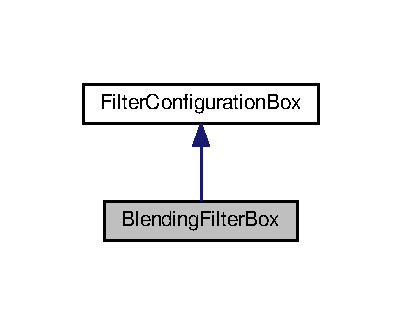
\includegraphics[width=193pt]{classGUI_1_1BlendingFilterBox__inherit__graph}
\end{center}
\end{figure}
\subsection*{Public Member Functions}
\begin{DoxyCompactItemize}
\item 
\hyperlink{classGUI_1_1BlendingFilterBox_a0aa76c7477d619b7738af743e0e5bb18}{Blending\+Filter\+Box} (\hyperlink{classGUI_1_1QWidget}{G\+U\+I\+::\+Q\+Widget} $\ast$parent)
\end{DoxyCompactItemize}
\subsection*{Additional Inherited Members}


\subsection{Detailed Description}
This class contains the gui elements for changing the options of a blending filter. 

\subsection{Constructor \& Destructor Documentation}
\hypertarget{classGUI_1_1BlendingFilterBox_a0aa76c7477d619b7738af743e0e5bb18}{}\index{G\+U\+I\+::\+Blending\+Filter\+Box@{G\+U\+I\+::\+Blending\+Filter\+Box}!Blending\+Filter\+Box@{Blending\+Filter\+Box}}
\index{Blending\+Filter\+Box@{Blending\+Filter\+Box}!G\+U\+I\+::\+Blending\+Filter\+Box@{G\+U\+I\+::\+Blending\+Filter\+Box}}
\subsubsection[{Blending\+Filter\+Box}]{\setlength{\rightskip}{0pt plus 5cm}{\bf Blending\+Filter\+Box} (
\begin{DoxyParamCaption}
\item[{{\bf G\+U\+I\+::\+Q\+Widget} $\ast$}]{parent}
\end{DoxyParamCaption}
)}\label{classGUI_1_1BlendingFilterBox_a0aa76c7477d619b7738af743e0e5bb18}


Constructor. 


\hypertarget{classModel_1_1Filter_1_1BlurFilter}{}\section{Blur\+Filter Class Reference}
\label{classModel_1_1Filter_1_1BlurFilter}\index{Blur\+Filter@{Blur\+Filter}}
\subsection*{Public Member Functions}
\begin{DoxyCompactItemize}
\item 
std\+::string \hyperlink{classModel_1_1Filter_1_1BlurFilter_a2b3f7d8fcd3d774b4a2fde5914a9729f}{get\+Filter\+Description} ()
\item 
\hypertarget{classModel_1_1Filter_1_1BlurFilter_a0f68baff76107f2b3982df5cca754340}{}bool {\bfseries get\+Preserve\+Edges} ()\label{classModel_1_1Filter_1_1BlurFilter_a0f68baff76107f2b3982df5cca754340}

\item 
\hypertarget{classModel_1_1Filter_1_1BlurFilter_a87c0326c6cec136fccffeca502d20ede}{}void {\bfseries set\+Preserve\+Edges} (bool preserve\+Edges)\label{classModel_1_1Filter_1_1BlurFilter_a87c0326c6cec136fccffeca502d20ede}

\item 
std\+::string \hyperlink{classModel_1_1Filter_1_1BlurFilter_ac0fc966d4386ddb71d99361e3fccb311}{get\+Name} ()
\item 
\hypertarget{classModel_1_1Filter_1_1BlurFilter_a708995fb1b6acb31ee0dfb0f4881e5b5}{}int {\bfseries get\+Intensity} ()\label{classModel_1_1Filter_1_1BlurFilter_a708995fb1b6acb31ee0dfb0f4881e5b5}

\item 
\hypertarget{classModel_1_1Filter_1_1BlurFilter_ac8255ffbc46bb61acaa8fd23d0d260eb}{}void {\bfseries set\+Intensity} (int intensity)\label{classModel_1_1Filter_1_1BlurFilter_ac8255ffbc46bb61acaa8fd23d0d260eb}

\end{DoxyCompactItemize}


\subsection{Detailed Description}
Blurs the video 

\subsection{Member Function Documentation}
\hypertarget{classModel_1_1Filter_1_1BlurFilter_a2b3f7d8fcd3d774b4a2fde5914a9729f}{}\index{Model\+::\+Filter\+::\+Blur\+Filter@{Model\+::\+Filter\+::\+Blur\+Filter}!get\+Filter\+Description@{get\+Filter\+Description}}
\index{get\+Filter\+Description@{get\+Filter\+Description}!Model\+::\+Filter\+::\+Blur\+Filter@{Model\+::\+Filter\+::\+Blur\+Filter}}
\subsubsection[{get\+Filter\+Description}]{\setlength{\rightskip}{0pt plus 5cm}std\+::string get\+Filter\+Description (
\begin{DoxyParamCaption}
{}
\end{DoxyParamCaption}
)\hspace{0.3cm}{\ttfamily [virtual]}}\label{classModel_1_1Filter_1_1BlurFilter_a2b3f7d8fcd3d774b4a2fde5914a9729f}


Returns the description of the filter 



Implements \hyperlink{classModel_1_1Filter_1_1Filter_ad400dc313dea3f9d3838d078ea4d2590}{Filter}.

\hypertarget{classModel_1_1Filter_1_1BlurFilter_ac0fc966d4386ddb71d99361e3fccb311}{}\index{Model\+::\+Filter\+::\+Blur\+Filter@{Model\+::\+Filter\+::\+Blur\+Filter}!get\+Name@{get\+Name}}
\index{get\+Name@{get\+Name}!Model\+::\+Filter\+::\+Blur\+Filter@{Model\+::\+Filter\+::\+Blur\+Filter}}
\subsubsection[{get\+Name}]{\setlength{\rightskip}{0pt plus 5cm}std\+::string get\+Name (
\begin{DoxyParamCaption}
{}
\end{DoxyParamCaption}
)\hspace{0.3cm}{\ttfamily [virtual]}}\label{classModel_1_1Filter_1_1BlurFilter_ac0fc966d4386ddb71d99361e3fccb311}


Returns the name of the filter 



Implements \hyperlink{classModel_1_1Filter_1_1Filter_ab7a5c5c512dadd4cbd18dd1b0f42e930}{Filter}.


\hypertarget{classGUI_1_1BlurFilterBox}{}\section{Blur\+Filter\+Box Class Reference}
\label{classGUI_1_1BlurFilterBox}\index{Blur\+Filter\+Box@{Blur\+Filter\+Box}}
\subsection*{Public Member Functions}
\begin{DoxyCompactItemize}
\item 
\hyperlink{classGUI_1_1BlurFilterBox_aa337b8816e06853cd7d6e64c3e4dd76b}{Blur\+Filter\+Box} (\hyperlink{classGUI_1_1Player_1_1QWidget}{G\+U\+I\+::\+Player\+::\+Q\+Widget} $\ast$parent)
\end{DoxyCompactItemize}
\subsection*{Additional Inherited Members}


\subsection{Detailed Description}
This class contains the gui elements for changing the options of a blurring filter. 

\subsection{Constructor \& Destructor Documentation}
\hypertarget{classGUI_1_1BlurFilterBox_aa337b8816e06853cd7d6e64c3e4dd76b}{}\index{G\+U\+I\+::\+Blur\+Filter\+Box@{G\+U\+I\+::\+Blur\+Filter\+Box}!Blur\+Filter\+Box@{Blur\+Filter\+Box}}
\index{Blur\+Filter\+Box@{Blur\+Filter\+Box}!G\+U\+I\+::\+Blur\+Filter\+Box@{G\+U\+I\+::\+Blur\+Filter\+Box}}
\subsubsection[{Blur\+Filter\+Box}]{\setlength{\rightskip}{0pt plus 5cm}{\bf Blur\+Filter\+Box} (
\begin{DoxyParamCaption}
\item[{{\bf G\+U\+I\+::\+Player\+::\+Q\+Widget} $\ast$}]{parent}
\end{DoxyParamCaption}
)}\label{classGUI_1_1BlurFilterBox_aa337b8816e06853cd7d6e64c3e4dd76b}


Constructor. 


\hypertarget{classModel_1_1Filter_1_1BorderFilter}{}\section{Border\+Filter Class Reference}
\label{classModel_1_1Filter_1_1BorderFilter}\index{Border\+Filter@{Border\+Filter}}
\subsection*{Public Member Functions}
\begin{DoxyCompactItemize}
\item 
std\+::string \hyperlink{classModel_1_1Filter_1_1BorderFilter_a2b3f7d8fcd3d774b4a2fde5914a9729f}{get\+Filter\+Description} ()
\item 
\hypertarget{classModel_1_1Filter_1_1BorderFilter_a7f662ce666098754b0916a828633f842}{}bool {\bfseries get\+Top} ()\label{classModel_1_1Filter_1_1BorderFilter_a7f662ce666098754b0916a828633f842}

\item 
\hypertarget{classModel_1_1Filter_1_1BorderFilter_a41a3d0253d877ec681fc30f85ae21aed}{}void {\bfseries set\+Top} (bool top)\label{classModel_1_1Filter_1_1BorderFilter_a41a3d0253d877ec681fc30f85ae21aed}

\item 
\hypertarget{classModel_1_1Filter_1_1BorderFilter_ac96fcca335b0daaa5e216993666a7af2}{}bool {\bfseries get\+Bottom} ()\label{classModel_1_1Filter_1_1BorderFilter_ac96fcca335b0daaa5e216993666a7af2}

\item 
\hypertarget{classModel_1_1Filter_1_1BorderFilter_ae60a4cf24fcd4cc34ca831917a609e79}{}void {\bfseries set\+Bottom} (bool bottom)\label{classModel_1_1Filter_1_1BorderFilter_ae60a4cf24fcd4cc34ca831917a609e79}

\item 
\hypertarget{classModel_1_1Filter_1_1BorderFilter_a09836b29d544b94e145dd6a725887dd2}{}bool {\bfseries get\+Right} ()\label{classModel_1_1Filter_1_1BorderFilter_a09836b29d544b94e145dd6a725887dd2}

\item 
std\+::string \hyperlink{classModel_1_1Filter_1_1BorderFilter_ac0fc966d4386ddb71d99361e3fccb311}{get\+Name} ()
\item 
\hypertarget{classModel_1_1Filter_1_1BorderFilter_a18165f5951ddba8f3b25b2a199f90bc1}{}void {\bfseries set\+Right} (bool right)\label{classModel_1_1Filter_1_1BorderFilter_a18165f5951ddba8f3b25b2a199f90bc1}

\item 
\hypertarget{classModel_1_1Filter_1_1BorderFilter_afb561071d09e3b031b1d951c51e94f24}{}bool {\bfseries get\+Left} ()\label{classModel_1_1Filter_1_1BorderFilter_afb561071d09e3b031b1d951c51e94f24}

\item 
\hypertarget{classModel_1_1Filter_1_1BorderFilter_a07821fa96843dccb8ee4c9a711f1f43b}{}void {\bfseries set\+Left} (bool left)\label{classModel_1_1Filter_1_1BorderFilter_a07821fa96843dccb8ee4c9a711f1f43b}

\item 
\hypertarget{classModel_1_1Filter_1_1BorderFilter_ab6b7bfb33162f992d1bb4e8d6699abef}{}int {\bfseries get\+Thickness} ()\label{classModel_1_1Filter_1_1BorderFilter_ab6b7bfb33162f992d1bb4e8d6699abef}

\item 
\hypertarget{classModel_1_1Filter_1_1BorderFilter_ae2faef96ee1277d229d6b6988c66e6d3}{}void {\bfseries set\+Thickness} (int thickness)\label{classModel_1_1Filter_1_1BorderFilter_ae2faef96ee1277d229d6b6988c66e6d3}

\item 
\hypertarget{classModel_1_1Filter_1_1BorderFilter_ae697defefbdf5f895406269b15758d91}{}Q\+Rgb {\bfseries get\+Color} ()\label{classModel_1_1Filter_1_1BorderFilter_ae697defefbdf5f895406269b15758d91}

\item 
\hypertarget{classModel_1_1Filter_1_1BorderFilter_ad858846447f303e473dc8004ef607666}{}void {\bfseries set\+Color} (Q\+Rgb color)\label{classModel_1_1Filter_1_1BorderFilter_ad858846447f303e473dc8004ef607666}

\end{DoxyCompactItemize}


\subsection{Detailed Description}
Inserts border into the video 

\subsection{Member Function Documentation}
\hypertarget{classModel_1_1Filter_1_1BorderFilter_a2b3f7d8fcd3d774b4a2fde5914a9729f}{}\index{Model\+::\+Filter\+::\+Border\+Filter@{Model\+::\+Filter\+::\+Border\+Filter}!get\+Filter\+Description@{get\+Filter\+Description}}
\index{get\+Filter\+Description@{get\+Filter\+Description}!Model\+::\+Filter\+::\+Border\+Filter@{Model\+::\+Filter\+::\+Border\+Filter}}
\subsubsection[{get\+Filter\+Description}]{\setlength{\rightskip}{0pt plus 5cm}std\+::string get\+Filter\+Description (
\begin{DoxyParamCaption}
{}
\end{DoxyParamCaption}
)\hspace{0.3cm}{\ttfamily [virtual]}}\label{classModel_1_1Filter_1_1BorderFilter_a2b3f7d8fcd3d774b4a2fde5914a9729f}


Returns the description of the filter 



Implements \hyperlink{classModel_1_1Filter_1_1Filter_ad400dc313dea3f9d3838d078ea4d2590}{Filter}.

\hypertarget{classModel_1_1Filter_1_1BorderFilter_ac0fc966d4386ddb71d99361e3fccb311}{}\index{Model\+::\+Filter\+::\+Border\+Filter@{Model\+::\+Filter\+::\+Border\+Filter}!get\+Name@{get\+Name}}
\index{get\+Name@{get\+Name}!Model\+::\+Filter\+::\+Border\+Filter@{Model\+::\+Filter\+::\+Border\+Filter}}
\subsubsection[{get\+Name}]{\setlength{\rightskip}{0pt plus 5cm}std\+::string get\+Name (
\begin{DoxyParamCaption}
{}
\end{DoxyParamCaption}
)\hspace{0.3cm}{\ttfamily [virtual]}}\label{classModel_1_1Filter_1_1BorderFilter_ac0fc966d4386ddb71d99361e3fccb311}


Returns the name of the filter 



Implements \hyperlink{classModel_1_1Filter_1_1Filter_ab7a5c5c512dadd4cbd18dd1b0f42e930}{Filter}.


\hypertarget{classGUI_1_1BorderFilterBox}{}\section{Border\+Filter\+Box Class Reference}
\label{classGUI_1_1BorderFilterBox}\index{Border\+Filter\+Box@{Border\+Filter\+Box}}


Inheritance diagram for Border\+Filter\+Box\+:
\nopagebreak
\begin{figure}[H]
\begin{center}
\leavevmode
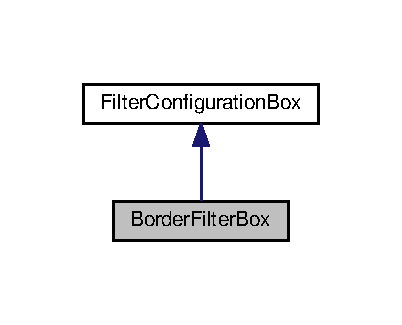
\includegraphics[width=193pt]{classGUI_1_1BorderFilterBox__inherit__graph}
\end{center}
\end{figure}
\subsection*{Public Member Functions}
\begin{DoxyCompactItemize}
\item 
\hyperlink{classGUI_1_1BorderFilterBox_a4b514b5fda573768947c8a82d79fa7b7}{Border\+Filter\+Box} (\hyperlink{classGUI_1_1QWidget}{G\+U\+I\+::\+Q\+Widget} $\ast$parent)
\end{DoxyCompactItemize}
\subsection*{Additional Inherited Members}


\subsection{Detailed Description}
This class contains the gui elements for changing the options of a border filter. 

\subsection{Constructor \& Destructor Documentation}
\hypertarget{classGUI_1_1BorderFilterBox_a4b514b5fda573768947c8a82d79fa7b7}{}\index{G\+U\+I\+::\+Border\+Filter\+Box@{G\+U\+I\+::\+Border\+Filter\+Box}!Border\+Filter\+Box@{Border\+Filter\+Box}}
\index{Border\+Filter\+Box@{Border\+Filter\+Box}!G\+U\+I\+::\+Border\+Filter\+Box@{G\+U\+I\+::\+Border\+Filter\+Box}}
\subsubsection[{Border\+Filter\+Box}]{\setlength{\rightskip}{0pt plus 5cm}{\bf Border\+Filter\+Box} (
\begin{DoxyParamCaption}
\item[{{\bf G\+U\+I\+::\+Q\+Widget} $\ast$}]{parent}
\end{DoxyParamCaption}
)}\label{classGUI_1_1BorderFilterBox_a4b514b5fda573768947c8a82d79fa7b7}


Constructor. 


\hypertarget{classModel_1_1Filter_1_1BrightnessFilter}{}\section{Brightness\+Filter Class Reference}
\label{classModel_1_1Filter_1_1BrightnessFilter}\index{Brightness\+Filter@{Brightness\+Filter}}
\subsection*{Public Member Functions}
\begin{DoxyCompactItemize}
\item 
\hyperlink{classModel_1_1Filter_1_1BrightnessFilter_a7be0e74d76ab6670dc2648d6833b9021}{Brightness\+Filter} ()
\item 
int \hyperlink{classModel_1_1Filter_1_1BrightnessFilter_a708995fb1b6acb31ee0dfb0f4881e5b5}{get\+Intensity} ()
\item 
void \hyperlink{classModel_1_1Filter_1_1BrightnessFilter_ac8255ffbc46bb61acaa8fd23d0d260eb}{set\+Intensity} (int intensity)
\item 
string \hyperlink{classModel_1_1Filter_1_1BrightnessFilter_a11335e13e50af74108bf926dc1340b4b}{get\+Name} ()
\item 
string \hyperlink{classModel_1_1Filter_1_1BrightnessFilter_a62b7b60e24f92234393b840b35808e06}{get\+Filter\+Description} ()
\end{DoxyCompactItemize}
\subsection*{Additional Inherited Members}


\subsection{Detailed Description}
Adjusts the video brightness. 

\subsection{Constructor \& Destructor Documentation}
\hypertarget{classModel_1_1Filter_1_1BrightnessFilter_a7be0e74d76ab6670dc2648d6833b9021}{}\index{Model\+::\+Filter\+::\+Brightness\+Filter@{Model\+::\+Filter\+::\+Brightness\+Filter}!Brightness\+Filter@{Brightness\+Filter}}
\index{Brightness\+Filter@{Brightness\+Filter}!Model\+::\+Filter\+::\+Brightness\+Filter@{Model\+::\+Filter\+::\+Brightness\+Filter}}
\subsubsection[{Brightness\+Filter}]{\setlength{\rightskip}{0pt plus 5cm}{\bf Brightness\+Filter} (
\begin{DoxyParamCaption}
{}
\end{DoxyParamCaption}
)}\label{classModel_1_1Filter_1_1BrightnessFilter_a7be0e74d76ab6670dc2648d6833b9021}


Constructor. 



\subsection{Member Function Documentation}
\hypertarget{classModel_1_1Filter_1_1BrightnessFilter_a62b7b60e24f92234393b840b35808e06}{}\index{Model\+::\+Filter\+::\+Brightness\+Filter@{Model\+::\+Filter\+::\+Brightness\+Filter}!get\+Filter\+Description@{get\+Filter\+Description}}
\index{get\+Filter\+Description@{get\+Filter\+Description}!Model\+::\+Filter\+::\+Brightness\+Filter@{Model\+::\+Filter\+::\+Brightness\+Filter}}
\subsubsection[{get\+Filter\+Description}]{\setlength{\rightskip}{0pt plus 5cm}string get\+Filter\+Description (
\begin{DoxyParamCaption}
{}
\end{DoxyParamCaption}
)\hspace{0.3cm}{\ttfamily [virtual]}}\label{classModel_1_1Filter_1_1BrightnessFilter_a62b7b60e24f92234393b840b35808e06}


Returns the string that the ffmpeg library needs to apply the filter to a video. 

\begin{DoxyReturn}{Returns}
The string for the ffmpeg library.
\end{DoxyReturn}


Implements \hyperlink{classModel_1_1Filter_1_1Filter_a453fcafa809afa1ce58d9ef95d5f26c0}{Filter}.

\hypertarget{classModel_1_1Filter_1_1BrightnessFilter_a708995fb1b6acb31ee0dfb0f4881e5b5}{}\index{Model\+::\+Filter\+::\+Brightness\+Filter@{Model\+::\+Filter\+::\+Brightness\+Filter}!get\+Intensity@{get\+Intensity}}
\index{get\+Intensity@{get\+Intensity}!Model\+::\+Filter\+::\+Brightness\+Filter@{Model\+::\+Filter\+::\+Brightness\+Filter}}
\subsubsection[{get\+Intensity}]{\setlength{\rightskip}{0pt plus 5cm}int get\+Intensity (
\begin{DoxyParamCaption}
{}
\end{DoxyParamCaption}
)}\label{classModel_1_1Filter_1_1BrightnessFilter_a708995fb1b6acb31ee0dfb0f4881e5b5}


Returns the intensity of the brightness. 

\begin{DoxyReturn}{Returns}
The intensity.
\end{DoxyReturn}
\hypertarget{classModel_1_1Filter_1_1BrightnessFilter_a11335e13e50af74108bf926dc1340b4b}{}\index{Model\+::\+Filter\+::\+Brightness\+Filter@{Model\+::\+Filter\+::\+Brightness\+Filter}!get\+Name@{get\+Name}}
\index{get\+Name@{get\+Name}!Model\+::\+Filter\+::\+Brightness\+Filter@{Model\+::\+Filter\+::\+Brightness\+Filter}}
\subsubsection[{get\+Name}]{\setlength{\rightskip}{0pt plus 5cm}string get\+Name (
\begin{DoxyParamCaption}
{}
\end{DoxyParamCaption}
)\hspace{0.3cm}{\ttfamily [virtual]}}\label{classModel_1_1Filter_1_1BrightnessFilter_a11335e13e50af74108bf926dc1340b4b}


Returns the name of the filter. 

\begin{DoxyReturn}{Returns}
The filtername.
\end{DoxyReturn}


Implements \hyperlink{classModel_1_1Filter_1_1Filter_ade93aa98c68d185a9c03784d36140225}{Filter}.

\hypertarget{classModel_1_1Filter_1_1BrightnessFilter_ac8255ffbc46bb61acaa8fd23d0d260eb}{}\index{Model\+::\+Filter\+::\+Brightness\+Filter@{Model\+::\+Filter\+::\+Brightness\+Filter}!set\+Intensity@{set\+Intensity}}
\index{set\+Intensity@{set\+Intensity}!Model\+::\+Filter\+::\+Brightness\+Filter@{Model\+::\+Filter\+::\+Brightness\+Filter}}
\subsubsection[{set\+Intensity}]{\setlength{\rightskip}{0pt plus 5cm}void set\+Intensity (
\begin{DoxyParamCaption}
\item[{int}]{intensity}
\end{DoxyParamCaption}
)}\label{classModel_1_1Filter_1_1BrightnessFilter_ac8255ffbc46bb61acaa8fd23d0d260eb}


Sets the intensity of the brightness. 


\begin{DoxyParams}{Parameters}
{\em intensity} & The new intensity.\\
\hline
\end{DoxyParams}

\hypertarget{classGUI_1_1BrightnessFilterBox}{}\section{Brightness\+Filter\+Box Class Reference}
\label{classGUI_1_1BrightnessFilterBox}\index{Brightness\+Filter\+Box@{Brightness\+Filter\+Box}}
\subsection*{Public Member Functions}
\begin{DoxyCompactItemize}
\item 
\hypertarget{classGUI_1_1BrightnessFilterBox_a37ebb44fb61750578debb2a51d2c00ce}{}{\bfseries Brightness\+Filter\+Box} (\hyperlink{classGUI_1_1QtGui_1_1QWidget____10}{G\+U\+I\+::\+Qt\+Gui\+::\+Q\+Widget\+\_\+\+\_\+10} $\ast$parent)\label{classGUI_1_1BrightnessFilterBox_a37ebb44fb61750578debb2a51d2c00ce}

\item 
\hypertarget{classGUI_1_1BrightnessFilterBox_ad7c0ee00fe3faac7942d75eec2a5342b}{}virtual void {\bfseries set\+Filter} (\hyperlink{classModel_1_1Filter_1_1Filter}{Model\+::\+Filter\+::\+Filter} \&filter)\label{classGUI_1_1BrightnessFilterBox_ad7c0ee00fe3faac7942d75eec2a5342b}

\item 
\hypertarget{classGUI_1_1BrightnessFilterBox_acef2029a93f4ab3a538cdb643b9c2613}{}virtual \hyperlink{classModel_1_1Filter_1_1Filter}{Model\+::\+Filter\+::\+Filter} $\ast$ {\bfseries get\+Filter} ()\label{classGUI_1_1BrightnessFilterBox_acef2029a93f4ab3a538cdb643b9c2613}

\end{DoxyCompactItemize}

\hypertarget{classModel_1_1Filter_1_1ColorbalanceFilter}{}\section{Colorbalance\+Filter Class Reference}
\label{classModel_1_1Filter_1_1ColorbalanceFilter}\index{Colorbalance\+Filter@{Colorbalance\+Filter}}
\subsection*{Public Member Functions}
\begin{DoxyCompactItemize}
\item 
std\+::string \hyperlink{classModel_1_1Filter_1_1ColorbalanceFilter_a2b3f7d8fcd3d774b4a2fde5914a9729f}{get\+Filter\+Description} ()
\item 
\hypertarget{classModel_1_1Filter_1_1ColorbalanceFilter_a82047004348409d221728e88c0b9dfa7}{}Model\+::\+Filter\+::\+Basic\+Color {\bfseries get\+Color} ()\label{classModel_1_1Filter_1_1ColorbalanceFilter_a82047004348409d221728e88c0b9dfa7}

\item 
\hypertarget{classModel_1_1Filter_1_1ColorbalanceFilter_a353ae5c263a046f9ef3b72438cfecd95}{}void {\bfseries set\+Color} (Model\+::\+Filter\+::\+Basic\+Color color)\label{classModel_1_1Filter_1_1ColorbalanceFilter_a353ae5c263a046f9ef3b72438cfecd95}

\item 
\hypertarget{classModel_1_1Filter_1_1ColorbalanceFilter_a708995fb1b6acb31ee0dfb0f4881e5b5}{}int {\bfseries get\+Intensity} ()\label{classModel_1_1Filter_1_1ColorbalanceFilter_a708995fb1b6acb31ee0dfb0f4881e5b5}

\item 
\hypertarget{classModel_1_1Filter_1_1ColorbalanceFilter_ac8255ffbc46bb61acaa8fd23d0d260eb}{}void {\bfseries set\+Intensity} (int intensity)\label{classModel_1_1Filter_1_1ColorbalanceFilter_ac8255ffbc46bb61acaa8fd23d0d260eb}

\item 
\hypertarget{classModel_1_1Filter_1_1ColorbalanceFilter_a1be0d343ed58d5d5bf7b816da375f190}{}bool {\bfseries get\+Bright\+Pixels} ()\label{classModel_1_1Filter_1_1ColorbalanceFilter_a1be0d343ed58d5d5bf7b816da375f190}

\item 
\hypertarget{classModel_1_1Filter_1_1ColorbalanceFilter_af0f286aa4c54fb1fd5813d02799da1cb}{}void {\bfseries set\+Bright\+Pixels} (bool bright\+Pixels)\label{classModel_1_1Filter_1_1ColorbalanceFilter_af0f286aa4c54fb1fd5813d02799da1cb}

\item 
\hypertarget{classModel_1_1Filter_1_1ColorbalanceFilter_a71d3e0e416aa251b66678a14b4bfa1a1}{}bool {\bfseries get\+Medium\+Pixels} ()\label{classModel_1_1Filter_1_1ColorbalanceFilter_a71d3e0e416aa251b66678a14b4bfa1a1}

\item 
\hypertarget{classModel_1_1Filter_1_1ColorbalanceFilter_ab52d8f4be21efb3dbc9ef49adf755ace}{}void {\bfseries set\+Medium\+Pixels} (bool medium\+Pixels)\label{classModel_1_1Filter_1_1ColorbalanceFilter_ab52d8f4be21efb3dbc9ef49adf755ace}

\item 
\hypertarget{classModel_1_1Filter_1_1ColorbalanceFilter_a81c4e5653e8217b741b4b183fe78abca}{}bool {\bfseries get\+Dark\+Pixels} ()\label{classModel_1_1Filter_1_1ColorbalanceFilter_a81c4e5653e8217b741b4b183fe78abca}

\item 
\hypertarget{classModel_1_1Filter_1_1ColorbalanceFilter_a0215d6818f471e2d3ba48b52c2c3da5d}{}void {\bfseries set\+Dark\+Pixels} (bool dark\+Pixels)\label{classModel_1_1Filter_1_1ColorbalanceFilter_a0215d6818f471e2d3ba48b52c2c3da5d}

\item 
virtual std\+::string \hyperlink{classModel_1_1Filter_1_1ColorbalanceFilter_ac0fc966d4386ddb71d99361e3fccb311}{get\+Name} ()
\end{DoxyCompactItemize}


\subsection{Detailed Description}
Adjusts the colorbalance of the video 

\subsection{Member Function Documentation}
\hypertarget{classModel_1_1Filter_1_1ColorbalanceFilter_a2b3f7d8fcd3d774b4a2fde5914a9729f}{}\index{Model\+::\+Filter\+::\+Colorbalance\+Filter@{Model\+::\+Filter\+::\+Colorbalance\+Filter}!get\+Filter\+Description@{get\+Filter\+Description}}
\index{get\+Filter\+Description@{get\+Filter\+Description}!Model\+::\+Filter\+::\+Colorbalance\+Filter@{Model\+::\+Filter\+::\+Colorbalance\+Filter}}
\subsubsection[{get\+Filter\+Description}]{\setlength{\rightskip}{0pt plus 5cm}std\+::string get\+Filter\+Description (
\begin{DoxyParamCaption}
{}
\end{DoxyParamCaption}
)\hspace{0.3cm}{\ttfamily [virtual]}}\label{classModel_1_1Filter_1_1ColorbalanceFilter_a2b3f7d8fcd3d774b4a2fde5914a9729f}


Returns the description of the filter 



Implements \hyperlink{classModel_1_1Filter_1_1Filter_ad400dc313dea3f9d3838d078ea4d2590}{Filter}.

\hypertarget{classModel_1_1Filter_1_1ColorbalanceFilter_ac0fc966d4386ddb71d99361e3fccb311}{}\index{Model\+::\+Filter\+::\+Colorbalance\+Filter@{Model\+::\+Filter\+::\+Colorbalance\+Filter}!get\+Name@{get\+Name}}
\index{get\+Name@{get\+Name}!Model\+::\+Filter\+::\+Colorbalance\+Filter@{Model\+::\+Filter\+::\+Colorbalance\+Filter}}
\subsubsection[{get\+Name}]{\setlength{\rightskip}{0pt plus 5cm}std\+::string get\+Name (
\begin{DoxyParamCaption}
{}
\end{DoxyParamCaption}
)\hspace{0.3cm}{\ttfamily [virtual]}}\label{classModel_1_1Filter_1_1ColorbalanceFilter_ac0fc966d4386ddb71d99361e3fccb311}


Returns the name of the filter 



Implements \hyperlink{classModel_1_1Filter_1_1Filter_ab7a5c5c512dadd4cbd18dd1b0f42e930}{Filter}.


\hypertarget{classGUI_1_1ColorbalanceFilterBox}{}\section{Colorbalance\+Filter\+Box Class Reference}
\label{classGUI_1_1ColorbalanceFilterBox}\index{Colorbalance\+Filter\+Box@{Colorbalance\+Filter\+Box}}
\subsection*{Public Member Functions}
\begin{DoxyCompactItemize}
\item 
\hyperlink{classGUI_1_1ColorbalanceFilterBox_ad9c200ecc17e1eec83f802fcb955d8b2}{Colorbalance\+Filter\+Box} (\hyperlink{classGUI_1_1Player_1_1QWidget}{G\+U\+I\+::\+Player\+::\+Q\+Widget} $\ast$parent)
\end{DoxyCompactItemize}
\subsection*{Additional Inherited Members}


\subsection{Detailed Description}
This class contains the gui elements for changing the options of a color balance filter. 

\subsection{Constructor \& Destructor Documentation}
\hypertarget{classGUI_1_1ColorbalanceFilterBox_ad9c200ecc17e1eec83f802fcb955d8b2}{}\index{G\+U\+I\+::\+Colorbalance\+Filter\+Box@{G\+U\+I\+::\+Colorbalance\+Filter\+Box}!Colorbalance\+Filter\+Box@{Colorbalance\+Filter\+Box}}
\index{Colorbalance\+Filter\+Box@{Colorbalance\+Filter\+Box}!G\+U\+I\+::\+Colorbalance\+Filter\+Box@{G\+U\+I\+::\+Colorbalance\+Filter\+Box}}
\subsubsection[{Colorbalance\+Filter\+Box}]{\setlength{\rightskip}{0pt plus 5cm}{\bf Colorbalance\+Filter\+Box} (
\begin{DoxyParamCaption}
\item[{{\bf G\+U\+I\+::\+Player\+::\+Q\+Widget} $\ast$}]{parent}
\end{DoxyParamCaption}
)}\label{classGUI_1_1ColorbalanceFilterBox_ad9c200ecc17e1eec83f802fcb955d8b2}


Constructor. 


\hypertarget{classModel_1_1Filter_1_1ContrastFilter}{}\section{Contrast\+Filter Class Reference}
\label{classModel_1_1Filter_1_1ContrastFilter}\index{Contrast\+Filter@{Contrast\+Filter}}
\subsection*{Public Member Functions}
\begin{DoxyCompactItemize}
\item 
std\+::string \hyperlink{classModel_1_1Filter_1_1ContrastFilter_a2b3f7d8fcd3d774b4a2fde5914a9729f}{get\+Filter\+Description} ()
\item 
\hypertarget{classModel_1_1Filter_1_1ContrastFilter_ac8255ffbc46bb61acaa8fd23d0d260eb}{}void {\bfseries set\+Intensity} (int intensity)\label{classModel_1_1Filter_1_1ContrastFilter_ac8255ffbc46bb61acaa8fd23d0d260eb}

\item 
\hypertarget{classModel_1_1Filter_1_1ContrastFilter_a708995fb1b6acb31ee0dfb0f4881e5b5}{}int {\bfseries get\+Intensity} ()\label{classModel_1_1Filter_1_1ContrastFilter_a708995fb1b6acb31ee0dfb0f4881e5b5}

\item 
std\+::string \hyperlink{classModel_1_1Filter_1_1ContrastFilter_ac0fc966d4386ddb71d99361e3fccb311}{get\+Name} ()
\end{DoxyCompactItemize}


\subsection{Detailed Description}
Adjusts the contrast of the video 

\subsection{Member Function Documentation}
\hypertarget{classModel_1_1Filter_1_1ContrastFilter_a2b3f7d8fcd3d774b4a2fde5914a9729f}{}\index{Model\+::\+Filter\+::\+Contrast\+Filter@{Model\+::\+Filter\+::\+Contrast\+Filter}!get\+Filter\+Description@{get\+Filter\+Description}}
\index{get\+Filter\+Description@{get\+Filter\+Description}!Model\+::\+Filter\+::\+Contrast\+Filter@{Model\+::\+Filter\+::\+Contrast\+Filter}}
\subsubsection[{get\+Filter\+Description}]{\setlength{\rightskip}{0pt plus 5cm}std\+::string get\+Filter\+Description (
\begin{DoxyParamCaption}
{}
\end{DoxyParamCaption}
)\hspace{0.3cm}{\ttfamily [virtual]}}\label{classModel_1_1Filter_1_1ContrastFilter_a2b3f7d8fcd3d774b4a2fde5914a9729f}


Returns the description of the filter 



Implements \hyperlink{classModel_1_1Filter_1_1Filter_ad400dc313dea3f9d3838d078ea4d2590}{Filter}.

\hypertarget{classModel_1_1Filter_1_1ContrastFilter_ac0fc966d4386ddb71d99361e3fccb311}{}\index{Model\+::\+Filter\+::\+Contrast\+Filter@{Model\+::\+Filter\+::\+Contrast\+Filter}!get\+Name@{get\+Name}}
\index{get\+Name@{get\+Name}!Model\+::\+Filter\+::\+Contrast\+Filter@{Model\+::\+Filter\+::\+Contrast\+Filter}}
\subsubsection[{get\+Name}]{\setlength{\rightskip}{0pt plus 5cm}std\+::string get\+Name (
\begin{DoxyParamCaption}
{}
\end{DoxyParamCaption}
)\hspace{0.3cm}{\ttfamily [virtual]}}\label{classModel_1_1Filter_1_1ContrastFilter_ac0fc966d4386ddb71d99361e3fccb311}


Returns the name of the filter 



Implements \hyperlink{classModel_1_1Filter_1_1Filter_ab7a5c5c512dadd4cbd18dd1b0f42e930}{Filter}.


\hypertarget{classGUI_1_1ContrastFilterBox}{}\section{Contrast\+Filter\+Box Class Reference}
\label{classGUI_1_1ContrastFilterBox}\index{Contrast\+Filter\+Box@{Contrast\+Filter\+Box}}


Inheritance diagram for Contrast\+Filter\+Box\+:
\nopagebreak
\begin{figure}[H]
\begin{center}
\leavevmode
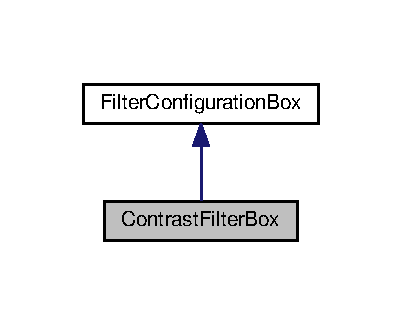
\includegraphics[width=193pt]{classGUI_1_1ContrastFilterBox__inherit__graph}
\end{center}
\end{figure}
\subsection*{Public Member Functions}
\begin{DoxyCompactItemize}
\item 
\hyperlink{classGUI_1_1ContrastFilterBox_a45a3637c1d2008b5631ae24e2419be1d}{Contrast\+Filter\+Box} (\hyperlink{classGUI_1_1QWidget}{G\+U\+I\+::\+Q\+Widget} $\ast$parent)
\end{DoxyCompactItemize}
\subsection*{Additional Inherited Members}


\subsection{Detailed Description}
This class contains the gui elements for changing the options of a contrast filter. 

\subsection{Constructor \& Destructor Documentation}
\hypertarget{classGUI_1_1ContrastFilterBox_a45a3637c1d2008b5631ae24e2419be1d}{}\index{G\+U\+I\+::\+Contrast\+Filter\+Box@{G\+U\+I\+::\+Contrast\+Filter\+Box}!Contrast\+Filter\+Box@{Contrast\+Filter\+Box}}
\index{Contrast\+Filter\+Box@{Contrast\+Filter\+Box}!G\+U\+I\+::\+Contrast\+Filter\+Box@{G\+U\+I\+::\+Contrast\+Filter\+Box}}
\subsubsection[{Contrast\+Filter\+Box}]{\setlength{\rightskip}{0pt plus 5cm}{\bf Contrast\+Filter\+Box} (
\begin{DoxyParamCaption}
\item[{{\bf G\+U\+I\+::\+Q\+Widget} $\ast$}]{parent}
\end{DoxyParamCaption}
)}\label{classGUI_1_1ContrastFilterBox_a45a3637c1d2008b5631ae24e2419be1d}


Constructor. 


\hypertarget{classGUI_1_1Player_1_1ControlPanel}{}\section{Control\+Panel Class Reference}
\label{classGUI_1_1Player_1_1ControlPanel}\index{Control\+Panel@{Control\+Panel}}
\subsection*{Public Member Functions}
\begin{DoxyCompactItemize}
\item 
\hyperlink{classGUI_1_1Player_1_1ControlPanel_a0efa607fe77b973e1128eae3bb33a9a1}{Control\+Panel} ()
\item 
void \hyperlink{classGUI_1_1Player_1_1ControlPanel_a798f5ffd7fe32e3fe8f67feed1e555c4}{set\+Master\+Video\+Player} (\hyperlink{classGUI_1_1Player_1_1Player}{Player\+::\+Player} \&player)
\item 
void \hyperlink{classGUI_1_1Player_1_1ControlPanel_ae904f1cf74c2473c9c548a255e67d88d}{add\+Video\+Player} (\hyperlink{classGUI_1_1Player_1_1Player}{G\+U\+I\+::\+Player\+::\+Player} \&player)
\item 
virtual void \hyperlink{classGUI_1_1Player_1_1ControlPanel_aa9963358cf9cff5ea2531d73efa78f73}{update\+Ui} ()=0
\item 
void \hyperlink{classGUI_1_1Player_1_1ControlPanel_aa24579c43e90697b0b05662270dfca3f}{remove\+Video\+Player} (\hyperlink{classGUI_1_1Player_1_1Player}{Player\+::\+Player} \&player)
\end{DoxyCompactItemize}
\subsection*{Data Fields}
\begin{DoxyCompactItemize}
\item 
\hyperlink{classGUI_1_1ForwardPlayer}{G\+U\+I\+::\+Forward\+Player} $\ast$ \hyperlink{classGUI_1_1Player_1_1ControlPanel_a15dc5e66f941f96f5b10d4da627f7f4e}{forward\+Panel}
\item 
\hyperlink{classGUI_1_1Player_1_1VideoPlayer}{G\+U\+I\+::\+Player\+::\+Video\+Player} $\ast$ \hyperlink{classGUI_1_1Player_1_1ControlPanel_a87e40dd85b4d49e1618debba5269e676}{master\+Panel}
\end{DoxyCompactItemize}
\subsection*{Protected Attributes}
\begin{DoxyCompactItemize}
\item 
std\+::vector$<$ \hyperlink{classGUI_1_1Player_1_1VideoPlayer}{G\+U\+I\+::\+Player\+::\+Video\+Player} $\ast$ $>$ \hyperlink{classGUI_1_1Player_1_1ControlPanel_a037ac66fc05dbb9755f983e0fe02ca80}{players}
\end{DoxyCompactItemize}


\subsection{Detailed Description}
This class is the base class for control panels. Control panels control videoplayers, 

\subsection{Constructor \& Destructor Documentation}
\hypertarget{classGUI_1_1Player_1_1ControlPanel_a0efa607fe77b973e1128eae3bb33a9a1}{}\index{G\+U\+I\+::\+Player\+::\+Control\+Panel@{G\+U\+I\+::\+Player\+::\+Control\+Panel}!Control\+Panel@{Control\+Panel}}
\index{Control\+Panel@{Control\+Panel}!G\+U\+I\+::\+Player\+::\+Control\+Panel@{G\+U\+I\+::\+Player\+::\+Control\+Panel}}
\subsubsection[{Control\+Panel}]{\setlength{\rightskip}{0pt plus 5cm}{\bf Control\+Panel} (
\begin{DoxyParamCaption}
{}
\end{DoxyParamCaption}
)}\label{classGUI_1_1Player_1_1ControlPanel_a0efa607fe77b973e1128eae3bb33a9a1}


Constructor. 



\subsection{Member Function Documentation}
\hypertarget{classGUI_1_1Player_1_1ControlPanel_ae904f1cf74c2473c9c548a255e67d88d}{}\index{G\+U\+I\+::\+Player\+::\+Control\+Panel@{G\+U\+I\+::\+Player\+::\+Control\+Panel}!add\+Video\+Player@{add\+Video\+Player}}
\index{add\+Video\+Player@{add\+Video\+Player}!G\+U\+I\+::\+Player\+::\+Control\+Panel@{G\+U\+I\+::\+Player\+::\+Control\+Panel}}
\subsubsection[{add\+Video\+Player}]{\setlength{\rightskip}{0pt plus 5cm}void add\+Video\+Player (
\begin{DoxyParamCaption}
\item[{{\bf G\+U\+I\+::\+Player\+::\+Player} \&}]{player}
\end{DoxyParamCaption}
)}\label{classGUI_1_1Player_1_1ControlPanel_ae904f1cf74c2473c9c548a255e67d88d}


Adds the video player the list of players to notify. 


\begin{DoxyParams}{Parameters}
{\em player} & The player to add to the list.\\
\hline
\end{DoxyParams}
\hypertarget{classGUI_1_1Player_1_1ControlPanel_aa24579c43e90697b0b05662270dfca3f}{}\index{G\+U\+I\+::\+Player\+::\+Control\+Panel@{G\+U\+I\+::\+Player\+::\+Control\+Panel}!remove\+Video\+Player@{remove\+Video\+Player}}
\index{remove\+Video\+Player@{remove\+Video\+Player}!G\+U\+I\+::\+Player\+::\+Control\+Panel@{G\+U\+I\+::\+Player\+::\+Control\+Panel}}
\subsubsection[{remove\+Video\+Player}]{\setlength{\rightskip}{0pt plus 5cm}void remove\+Video\+Player (
\begin{DoxyParamCaption}
\item[{{\bf Player\+::\+Player} \&}]{player}
\end{DoxyParamCaption}
)}\label{classGUI_1_1Player_1_1ControlPanel_aa24579c43e90697b0b05662270dfca3f}


Removes the video player from the list of the players to notify. 


\begin{DoxyParams}{Parameters}
{\em player} & The player to remove.\\
\hline
\end{DoxyParams}
\hypertarget{classGUI_1_1Player_1_1ControlPanel_a798f5ffd7fe32e3fe8f67feed1e555c4}{}\index{G\+U\+I\+::\+Player\+::\+Control\+Panel@{G\+U\+I\+::\+Player\+::\+Control\+Panel}!set\+Master\+Video\+Player@{set\+Master\+Video\+Player}}
\index{set\+Master\+Video\+Player@{set\+Master\+Video\+Player}!G\+U\+I\+::\+Player\+::\+Control\+Panel@{G\+U\+I\+::\+Player\+::\+Control\+Panel}}
\subsubsection[{set\+Master\+Video\+Player}]{\setlength{\rightskip}{0pt plus 5cm}void set\+Master\+Video\+Player (
\begin{DoxyParamCaption}
\item[{{\bf Player\+::\+Player} \&}]{player}
\end{DoxyParamCaption}
)}\label{classGUI_1_1Player_1_1ControlPanel_a798f5ffd7fe32e3fe8f67feed1e555c4}


Sets the master video player. The master video player is the reference to where to set the position of the slider, if the video is played paused or stopped. 


\begin{DoxyParams}{Parameters}
{\em player} & The master video player.\\
\hline
\end{DoxyParams}
\hypertarget{classGUI_1_1Player_1_1ControlPanel_aa9963358cf9cff5ea2531d73efa78f73}{}\index{G\+U\+I\+::\+Player\+::\+Control\+Panel@{G\+U\+I\+::\+Player\+::\+Control\+Panel}!update\+Ui@{update\+Ui}}
\index{update\+Ui@{update\+Ui}!G\+U\+I\+::\+Player\+::\+Control\+Panel@{G\+U\+I\+::\+Player\+::\+Control\+Panel}}
\subsubsection[{update\+Ui}]{\setlength{\rightskip}{0pt plus 5cm}virtual void update\+Ui (
\begin{DoxyParamCaption}
{}
\end{DoxyParamCaption}
)\hspace{0.3cm}{\ttfamily [pure virtual]}}\label{classGUI_1_1Player_1_1ControlPanel_aa9963358cf9cff5ea2531d73efa78f73}


Updates the ui of the control panel. 



Implemented in \hyperlink{classGUI_1_1Player_1_1PlayerControlPanel_ae13c7f95f1ceda0fec18d18c3d7619f6}{Player\+Control\+Panel}, \hyperlink{classGUI_1_1Player_1_1PreviewControlPanel_ae13c7f95f1ceda0fec18d18c3d7619f6}{Preview\+Control\+Panel}, and \hyperlink{classGUI_1_1GlobalControlPanel_ae13c7f95f1ceda0fec18d18c3d7619f6}{Global\+Control\+Panel}.



\subsection{Field Documentation}
\hypertarget{classGUI_1_1Player_1_1ControlPanel_a15dc5e66f941f96f5b10d4da627f7f4e}{}\index{G\+U\+I\+::\+Player\+::\+Control\+Panel@{G\+U\+I\+::\+Player\+::\+Control\+Panel}!forward\+Panel@{forward\+Panel}}
\index{forward\+Panel@{forward\+Panel}!G\+U\+I\+::\+Player\+::\+Control\+Panel@{G\+U\+I\+::\+Player\+::\+Control\+Panel}}
\subsubsection[{forward\+Panel}]{\setlength{\rightskip}{0pt plus 5cm}{\bf G\+U\+I\+::\+Forward\+Player}$\ast$ forward\+Panel}\label{classGUI_1_1Player_1_1ControlPanel_a15dc5e66f941f96f5b10d4da627f7f4e}
\hypertarget{classGUI_1_1Player_1_1ControlPanel_a87e40dd85b4d49e1618debba5269e676}{}\index{G\+U\+I\+::\+Player\+::\+Control\+Panel@{G\+U\+I\+::\+Player\+::\+Control\+Panel}!master\+Panel@{master\+Panel}}
\index{master\+Panel@{master\+Panel}!G\+U\+I\+::\+Player\+::\+Control\+Panel@{G\+U\+I\+::\+Player\+::\+Control\+Panel}}
\subsubsection[{master\+Panel}]{\setlength{\rightskip}{0pt plus 5cm}{\bf G\+U\+I\+::\+Player\+::\+Video\+Player}$\ast$ master\+Panel}\label{classGUI_1_1Player_1_1ControlPanel_a87e40dd85b4d49e1618debba5269e676}
\hypertarget{classGUI_1_1Player_1_1ControlPanel_a037ac66fc05dbb9755f983e0fe02ca80}{}\index{G\+U\+I\+::\+Player\+::\+Control\+Panel@{G\+U\+I\+::\+Player\+::\+Control\+Panel}!players@{players}}
\index{players@{players}!G\+U\+I\+::\+Player\+::\+Control\+Panel@{G\+U\+I\+::\+Player\+::\+Control\+Panel}}
\subsubsection[{players}]{\setlength{\rightskip}{0pt plus 5cm}std\+::vector$<${\bf G\+U\+I\+::\+Player\+::\+Video\+Player}$\ast$$>$ players\hspace{0.3cm}{\ttfamily [protected]}}\label{classGUI_1_1Player_1_1ControlPanel_a037ac66fc05dbb9755f983e0fe02ca80}

\hypertarget{classModel_1_1Filter_1_1EdgeFilter}{}\section{Edge\+Filter Class Reference}
\label{classModel_1_1Filter_1_1EdgeFilter}\index{Edge\+Filter@{Edge\+Filter}}
\subsection*{Public Member Functions}
\begin{DoxyCompactItemize}
\item 
std\+::string \hyperlink{classModel_1_1Filter_1_1EdgeFilter_a2b3f7d8fcd3d774b4a2fde5914a9729f}{get\+Filter\+Description} ()
\item 
std\+::string \hyperlink{classModel_1_1Filter_1_1EdgeFilter_ac0fc966d4386ddb71d99361e3fccb311}{get\+Name} ()
\end{DoxyCompactItemize}


\subsection{Detailed Description}
Only shows the borders and places a black overlay over the rest 

\subsection{Member Function Documentation}
\hypertarget{classModel_1_1Filter_1_1EdgeFilter_a2b3f7d8fcd3d774b4a2fde5914a9729f}{}\index{Model\+::\+Filter\+::\+Edge\+Filter@{Model\+::\+Filter\+::\+Edge\+Filter}!get\+Filter\+Description@{get\+Filter\+Description}}
\index{get\+Filter\+Description@{get\+Filter\+Description}!Model\+::\+Filter\+::\+Edge\+Filter@{Model\+::\+Filter\+::\+Edge\+Filter}}
\subsubsection[{get\+Filter\+Description}]{\setlength{\rightskip}{0pt plus 5cm}std\+::string get\+Filter\+Description (
\begin{DoxyParamCaption}
{}
\end{DoxyParamCaption}
)\hspace{0.3cm}{\ttfamily [virtual]}}\label{classModel_1_1Filter_1_1EdgeFilter_a2b3f7d8fcd3d774b4a2fde5914a9729f}


Returns the description of the filter 



Implements \hyperlink{classModel_1_1Filter_1_1Filter_ad400dc313dea3f9d3838d078ea4d2590}{Filter}.

\hypertarget{classModel_1_1Filter_1_1EdgeFilter_ac0fc966d4386ddb71d99361e3fccb311}{}\index{Model\+::\+Filter\+::\+Edge\+Filter@{Model\+::\+Filter\+::\+Edge\+Filter}!get\+Name@{get\+Name}}
\index{get\+Name@{get\+Name}!Model\+::\+Filter\+::\+Edge\+Filter@{Model\+::\+Filter\+::\+Edge\+Filter}}
\subsubsection[{get\+Name}]{\setlength{\rightskip}{0pt plus 5cm}std\+::string get\+Name (
\begin{DoxyParamCaption}
{}
\end{DoxyParamCaption}
)\hspace{0.3cm}{\ttfamily [virtual]}}\label{classModel_1_1Filter_1_1EdgeFilter_ac0fc966d4386ddb71d99361e3fccb311}


Returns the name of the filter 



Implements \hyperlink{classModel_1_1Filter_1_1Filter_ab7a5c5c512dadd4cbd18dd1b0f42e930}{Filter}.


\hypertarget{classGUI_1_1EdgeFilterBox}{}\section{Edge\+Filter\+Box Class Reference}
\label{classGUI_1_1EdgeFilterBox}\index{Edge\+Filter\+Box@{Edge\+Filter\+Box}}
\subsection*{Public Member Functions}
\begin{DoxyCompactItemize}
\item 
\hypertarget{classGUI_1_1EdgeFilterBox_a829283d1074efd29172c6c9a2e769f6b}{}{\bfseries Edge\+Filter\+Box} (\hyperlink{classGUI_1_1QtGui_1_1QWidget____10}{G\+U\+I\+::\+Qt\+Gui\+::\+Q\+Widget\+\_\+\+\_\+10} $\ast$parent)\label{classGUI_1_1EdgeFilterBox_a829283d1074efd29172c6c9a2e769f6b}

\item 
\hypertarget{classGUI_1_1EdgeFilterBox_ad7c0ee00fe3faac7942d75eec2a5342b}{}virtual void {\bfseries set\+Filter} (\hyperlink{classModel_1_1Filter_1_1Filter}{Model\+::\+Filter\+::\+Filter} \&filter)\label{classGUI_1_1EdgeFilterBox_ad7c0ee00fe3faac7942d75eec2a5342b}

\item 
\hypertarget{classGUI_1_1EdgeFilterBox_acef2029a93f4ab3a538cdb643b9c2613}{}virtual \hyperlink{classModel_1_1Filter_1_1Filter}{Model\+::\+Filter\+::\+Filter} $\ast$ {\bfseries get\+Filter} ()\label{classGUI_1_1EdgeFilterBox_acef2029a93f4ab3a538cdb643b9c2613}

\end{DoxyCompactItemize}

\hypertarget{classModel_1_1EncodedVideo}{}\section{Encoded\+Video Class Reference}
\label{classModel_1_1EncodedVideo}\index{Encoded\+Video@{Encoded\+Video}}
\subsection*{Public Member Functions}
\begin{DoxyCompactItemize}
\item 
\hyperlink{classModel_1_1EncodedVideo_a436d811c3c2420e132a2b4e04959c5de}{Encoded\+Video} (Q\+String path)
\item 
Q\+String \hyperlink{classModel_1_1EncodedVideo_a1a94d0c9bf9dd725556721ac914025e3}{get\+Path} ()
\item 
int \hyperlink{classModel_1_1EncodedVideo_ac4465cfb146410e557acc4892afd9e7c}{get\+File\+Size} ()
\item 
int \hyperlink{classModel_1_1EncodedVideo_ab9202ba7e871cc8488f73a14e4e6abef}{get\+Number\+Of\+Colors} ()
\item 
Q\+String \hyperlink{classModel_1_1EncodedVideo_ad0b9ca84489c31d0155646495380ac0b}{get\+Codec} ()
\item 
\hyperlink{classModel_1_1Graph}{Model\+::\+Graph} \& \hyperlink{classModel_1_1EncodedVideo_afe6efbe8e2d7312d31f9df848685c2a1}{get\+Bitrate} ()
\item 
\hyperlink{classModel_1_1Graph}{Model\+::\+Graph} \& \hyperlink{classModel_1_1EncodedVideo_a4c4816fa0fc4d120b7ca4727f92b8434}{get\+Psnr} ()
\item 
\hyperlink{classModel_1_1Graph}{Model\+::\+Graph} \& \hyperlink{classModel_1_1EncodedVideo_a2e964007d3803c23555685e582f1f8f8}{get\+Red\+Histogramm} ()
\item 
\hyperlink{classModel_1_1Graph}{Model\+::\+Graph} \& \hyperlink{classModel_1_1EncodedVideo_a665006efad68684718c78c213e081f16}{get\+Blue\+Histogramm} ()
\item 
\hyperlink{classModel_1_1Graph}{Model\+::\+Graph} \& \hyperlink{classModel_1_1EncodedVideo_a85d21a1922c274ff928b8794627fc3f0}{get\+Green\+Histogramm} ()
\item 
\hyperlink{classModel_1_1AVVideo}{Model\+::\+A\+V\+Video} \& \hyperlink{classModel_1_1EncodedVideo_a58bd43e5cbaa711bf19b0c71efbc9834}{get\+Av\+Video} ()
\item 
\hyperlink{classGUI_1_1Player_1_1Video}{G\+U\+I\+::\+Player\+::\+Video} \& \hyperlink{classModel_1_1EncodedVideo_a8efa1486dd7b968e9b0f1cb5be919381}{get\+Macro\+Block\+Video} ()
\item 
\hyperlink{classGUI_1_1Player_1_1Video}{G\+U\+I\+::\+Player\+::\+Video} \& \hyperlink{classModel_1_1EncodedVideo_a85eb47f3e866632f0e48c89becc72d1a}{get\+Rgb\+Diff\+Video} (\hyperlink{classGUI_1_1Player_1_1Video}{G\+U\+I\+::\+Player\+::\+Video} $\ast$reference=0)
\item 
\hyperlink{classGUI_1_1Player_1_1Video}{G\+U\+I\+::\+Player\+::\+Video} \& \hyperlink{classModel_1_1EncodedVideo_a56ebcfcff7dfad1f4b9e302794451afe}{get\+Video} ()
\item 
void \hyperlink{classModel_1_1EncodedVideo_a60a6dd2db95a7b5512b119592154c542}{set\+Bitrate} (\hyperlink{classModel_1_1Graph}{Model\+::\+Graph} graph)
\item 
void \hyperlink{classModel_1_1EncodedVideo_a1ab9a88bf6af5d5c764512703becc453}{set\+Psnr} (\hyperlink{classModel_1_1Graph}{Model\+::\+Graph} graph)
\item 
void \hyperlink{classModel_1_1EncodedVideo_a50a774bf6d0a0445ad71fce4030f923b}{set\+Red\+Histogramm} (\hyperlink{classModel_1_1Graph}{Model\+::\+Graph} graph)
\item 
void \hyperlink{classModel_1_1EncodedVideo_a566ac8c5c38d5e9ff92033d425ad1af5}{set\+Green\+Histogramm} (\hyperlink{classModel_1_1Graph}{Model\+::\+Graph} graph)
\item 
void \hyperlink{classModel_1_1EncodedVideo_a73e0e302836a23164bc5fafc2efcb412}{set\+Blue\+Histogramm} (\hyperlink{classModel_1_1Graph}{Model\+::\+Graph} graph)
\item 
void \hyperlink{classModel_1_1EncodedVideo_aa7f8f6cccdf2b783931981c42c093fe5}{set\+Macroblock\+Video} (\hyperlink{classGUI_1_1Player_1_1Video}{G\+U\+I\+::\+Player\+::\+Video} \hyperlink{classModel_1_1EncodedVideo_a03e0f42a43f7a856dd9881df4024fb4c}{video})
\item 
void \hyperlink{classModel_1_1EncodedVideo_a9f858252aac3af726c1ba68f580321f9}{set\+Rgb\+Diff\+Video} (\hyperlink{classGUI_1_1Player_1_1Video}{G\+U\+I\+::\+Player\+::\+Video} \hyperlink{classModel_1_1EncodedVideo_a03e0f42a43f7a856dd9881df4024fb4c}{video})
\end{DoxyCompactItemize}
\subsection*{Data Fields}
\begin{DoxyCompactItemize}
\item 
\hyperlink{classGUI_1_1AnalysisBox}{G\+U\+I\+::\+Analysis\+Box} $\ast$ \hyperlink{classModel_1_1EncodedVideo_a03e0f42a43f7a856dd9881df4024fb4c}{video}
\item 
\hyperlink{classModel_1_1AVVideo}{Model\+::\+A\+V\+Video} $\ast$ \hyperlink{classModel_1_1EncodedVideo_a270efc836b2d2c70aec72106128ff89f}{av\+Video}
\item 
\hyperlink{classGUI_1_1Player_1_1Video}{G\+U\+I\+::\+Player\+::\+Video} $\ast$ \hyperlink{classModel_1_1EncodedVideo_a17f257b55491782940deb4e086adecbb}{display\+Video}
\item 
\hyperlink{classGUI_1_1Player_1_1Video}{G\+U\+I\+::\+Player\+::\+Video} $\ast$ \hyperlink{classModel_1_1EncodedVideo_afb2db9bff47ddb8b0d279068e7b24444}{macroblock\+Video}
\item 
\hyperlink{classGUI_1_1Player_1_1Video}{G\+U\+I\+::\+Player\+::\+Video} $\ast$ \hyperlink{classModel_1_1EncodedVideo_a0a3659e25658447f14c6c00399888369}{rgb\+Diff\+Video}
\item 
\hyperlink{classModel_1_1Graph}{Model\+::\+Graph} $\ast$ \hyperlink{classModel_1_1EncodedVideo_aec2e020f785ceb00064fb8033826603e}{bitrate}
\item 
\hyperlink{classModel_1_1Graph}{Model\+::\+Graph} $\ast$ \hyperlink{classModel_1_1EncodedVideo_a9bac82e3934ef7816be95e35cd18c852}{psnr}
\item 
\hyperlink{classModel_1_1Graph}{Model\+::\+Graph} $\ast$ \hyperlink{classModel_1_1EncodedVideo_a687c8a2518054613e946c48f33520458}{red\+Histo}
\item 
\hyperlink{classModel_1_1Graph}{Model\+::\+Graph} $\ast$ \hyperlink{classModel_1_1EncodedVideo_af09ff3f1ad12186cc33f3ab4cb146cdb}{green\+Histo}
\item 
\hyperlink{classModel_1_1Graph}{Model\+::\+Graph} $\ast$ \hyperlink{classModel_1_1EncodedVideo_a53ce36c444026a777d53d7c2d872b059}{blue\+Hiso}
\end{DoxyCompactItemize}


\subsection{Detailed Description}
This class contains all analysis info of a encoded video. 

\subsection{Constructor \& Destructor Documentation}
\hypertarget{classModel_1_1EncodedVideo_a436d811c3c2420e132a2b4e04959c5de}{}\index{Model\+::\+Encoded\+Video@{Model\+::\+Encoded\+Video}!Encoded\+Video@{Encoded\+Video}}
\index{Encoded\+Video@{Encoded\+Video}!Model\+::\+Encoded\+Video@{Model\+::\+Encoded\+Video}}
\subsubsection[{Encoded\+Video}]{\setlength{\rightskip}{0pt plus 5cm}{\bf Encoded\+Video} (
\begin{DoxyParamCaption}
\item[{Q\+String}]{path}
\end{DoxyParamCaption}
)}\label{classModel_1_1EncodedVideo_a436d811c3c2420e132a2b4e04959c5de}


Constructor. 


\begin{DoxyParams}{Parameters}
{\em path} & Path to the video.\\
\hline
\end{DoxyParams}


\subsection{Member Function Documentation}
\hypertarget{classModel_1_1EncodedVideo_a58bd43e5cbaa711bf19b0c71efbc9834}{}\index{Model\+::\+Encoded\+Video@{Model\+::\+Encoded\+Video}!get\+Av\+Video@{get\+Av\+Video}}
\index{get\+Av\+Video@{get\+Av\+Video}!Model\+::\+Encoded\+Video@{Model\+::\+Encoded\+Video}}
\subsubsection[{get\+Av\+Video}]{\setlength{\rightskip}{0pt plus 5cm}{\bf Model\+::\+A\+V\+Video} \& get\+Av\+Video (
\begin{DoxyParamCaption}
{}
\end{DoxyParamCaption}
)}\label{classModel_1_1EncodedVideo_a58bd43e5cbaa711bf19b0c71efbc9834}


Returns the \hyperlink{classModel_1_1AVVideo}{A\+V\+Video}. 

\begin{DoxyReturn}{Returns}
The \hyperlink{classModel_1_1AVVideo}{A\+V\+Video}.
\end{DoxyReturn}
\hypertarget{classModel_1_1EncodedVideo_afe6efbe8e2d7312d31f9df848685c2a1}{}\index{Model\+::\+Encoded\+Video@{Model\+::\+Encoded\+Video}!get\+Bitrate@{get\+Bitrate}}
\index{get\+Bitrate@{get\+Bitrate}!Model\+::\+Encoded\+Video@{Model\+::\+Encoded\+Video}}
\subsubsection[{get\+Bitrate}]{\setlength{\rightskip}{0pt plus 5cm}{\bf Model\+::\+Graph} \& get\+Bitrate (
\begin{DoxyParamCaption}
{}
\end{DoxyParamCaption}
)}\label{classModel_1_1EncodedVideo_afe6efbe8e2d7312d31f9df848685c2a1}


Returns the bitrate graph. 

\begin{DoxyReturn}{Returns}
The bitrate graph.
\end{DoxyReturn}
\hypertarget{classModel_1_1EncodedVideo_a665006efad68684718c78c213e081f16}{}\index{Model\+::\+Encoded\+Video@{Model\+::\+Encoded\+Video}!get\+Blue\+Histogramm@{get\+Blue\+Histogramm}}
\index{get\+Blue\+Histogramm@{get\+Blue\+Histogramm}!Model\+::\+Encoded\+Video@{Model\+::\+Encoded\+Video}}
\subsubsection[{get\+Blue\+Histogramm}]{\setlength{\rightskip}{0pt plus 5cm}{\bf Model\+::\+Graph} \& get\+Blue\+Histogramm (
\begin{DoxyParamCaption}
{}
\end{DoxyParamCaption}
)}\label{classModel_1_1EncodedVideo_a665006efad68684718c78c213e081f16}


Returns the blue histogramm graph. 

\begin{DoxyReturn}{Returns}
The blue histogramm.
\end{DoxyReturn}
\hypertarget{classModel_1_1EncodedVideo_ad0b9ca84489c31d0155646495380ac0b}{}\index{Model\+::\+Encoded\+Video@{Model\+::\+Encoded\+Video}!get\+Codec@{get\+Codec}}
\index{get\+Codec@{get\+Codec}!Model\+::\+Encoded\+Video@{Model\+::\+Encoded\+Video}}
\subsubsection[{get\+Codec}]{\setlength{\rightskip}{0pt plus 5cm}Q\+String get\+Codec (
\begin{DoxyParamCaption}
{}
\end{DoxyParamCaption}
)}\label{classModel_1_1EncodedVideo_ad0b9ca84489c31d0155646495380ac0b}


Returns the codec used in the video file. 

\begin{DoxyReturn}{Returns}
The used codec.
\end{DoxyReturn}
\hypertarget{classModel_1_1EncodedVideo_ac4465cfb146410e557acc4892afd9e7c}{}\index{Model\+::\+Encoded\+Video@{Model\+::\+Encoded\+Video}!get\+File\+Size@{get\+File\+Size}}
\index{get\+File\+Size@{get\+File\+Size}!Model\+::\+Encoded\+Video@{Model\+::\+Encoded\+Video}}
\subsubsection[{get\+File\+Size}]{\setlength{\rightskip}{0pt plus 5cm}int get\+File\+Size (
\begin{DoxyParamCaption}
{}
\end{DoxyParamCaption}
)}\label{classModel_1_1EncodedVideo_ac4465cfb146410e557acc4892afd9e7c}


Returns the size of the video file. 

\begin{DoxyReturn}{Returns}
the file size.
\end{DoxyReturn}
\hypertarget{classModel_1_1EncodedVideo_a85d21a1922c274ff928b8794627fc3f0}{}\index{Model\+::\+Encoded\+Video@{Model\+::\+Encoded\+Video}!get\+Green\+Histogramm@{get\+Green\+Histogramm}}
\index{get\+Green\+Histogramm@{get\+Green\+Histogramm}!Model\+::\+Encoded\+Video@{Model\+::\+Encoded\+Video}}
\subsubsection[{get\+Green\+Histogramm}]{\setlength{\rightskip}{0pt plus 5cm}{\bf Model\+::\+Graph} \& get\+Green\+Histogramm (
\begin{DoxyParamCaption}
{}
\end{DoxyParamCaption}
)}\label{classModel_1_1EncodedVideo_a85d21a1922c274ff928b8794627fc3f0}


Returns the green histogramm graph. 

\begin{DoxyReturn}{Returns}
The green histogramm.
\end{DoxyReturn}
\hypertarget{classModel_1_1EncodedVideo_a8efa1486dd7b968e9b0f1cb5be919381}{}\index{Model\+::\+Encoded\+Video@{Model\+::\+Encoded\+Video}!get\+Macro\+Block\+Video@{get\+Macro\+Block\+Video}}
\index{get\+Macro\+Block\+Video@{get\+Macro\+Block\+Video}!Model\+::\+Encoded\+Video@{Model\+::\+Encoded\+Video}}
\subsubsection[{get\+Macro\+Block\+Video}]{\setlength{\rightskip}{0pt plus 5cm}{\bf G\+U\+I\+::\+Player\+::\+Video} \& get\+Macro\+Block\+Video (
\begin{DoxyParamCaption}
{}
\end{DoxyParamCaption}
)}\label{classModel_1_1EncodedVideo_a8efa1486dd7b968e9b0f1cb5be919381}


Returns the video which shows the macroblocks. 

\begin{DoxyReturn}{Returns}
The macroblock video.
\end{DoxyReturn}
\hypertarget{classModel_1_1EncodedVideo_ab9202ba7e871cc8488f73a14e4e6abef}{}\index{Model\+::\+Encoded\+Video@{Model\+::\+Encoded\+Video}!get\+Number\+Of\+Colors@{get\+Number\+Of\+Colors}}
\index{get\+Number\+Of\+Colors@{get\+Number\+Of\+Colors}!Model\+::\+Encoded\+Video@{Model\+::\+Encoded\+Video}}
\subsubsection[{get\+Number\+Of\+Colors}]{\setlength{\rightskip}{0pt plus 5cm}int get\+Number\+Of\+Colors (
\begin{DoxyParamCaption}
{}
\end{DoxyParamCaption}
)}\label{classModel_1_1EncodedVideo_ab9202ba7e871cc8488f73a14e4e6abef}


Returns the number of colors that appear in the whole video. 

\begin{DoxyReturn}{Returns}
The number of colors in the video.
\end{DoxyReturn}
\hypertarget{classModel_1_1EncodedVideo_a1a94d0c9bf9dd725556721ac914025e3}{}\index{Model\+::\+Encoded\+Video@{Model\+::\+Encoded\+Video}!get\+Path@{get\+Path}}
\index{get\+Path@{get\+Path}!Model\+::\+Encoded\+Video@{Model\+::\+Encoded\+Video}}
\subsubsection[{get\+Path}]{\setlength{\rightskip}{0pt plus 5cm}Q\+String get\+Path (
\begin{DoxyParamCaption}
{}
\end{DoxyParamCaption}
)}\label{classModel_1_1EncodedVideo_a1a94d0c9bf9dd725556721ac914025e3}


Returns the path to the video. 

\begin{DoxyReturn}{Returns}
The path to the video.
\end{DoxyReturn}
\hypertarget{classModel_1_1EncodedVideo_a4c4816fa0fc4d120b7ca4727f92b8434}{}\index{Model\+::\+Encoded\+Video@{Model\+::\+Encoded\+Video}!get\+Psnr@{get\+Psnr}}
\index{get\+Psnr@{get\+Psnr}!Model\+::\+Encoded\+Video@{Model\+::\+Encoded\+Video}}
\subsubsection[{get\+Psnr}]{\setlength{\rightskip}{0pt plus 5cm}{\bf Model\+::\+Graph} \& get\+Psnr (
\begin{DoxyParamCaption}
{}
\end{DoxyParamCaption}
)}\label{classModel_1_1EncodedVideo_a4c4816fa0fc4d120b7ca4727f92b8434}


Returns the psnr graph. 

\begin{DoxyReturn}{Returns}
The psnr graph.
\end{DoxyReturn}
\hypertarget{classModel_1_1EncodedVideo_a2e964007d3803c23555685e582f1f8f8}{}\index{Model\+::\+Encoded\+Video@{Model\+::\+Encoded\+Video}!get\+Red\+Histogramm@{get\+Red\+Histogramm}}
\index{get\+Red\+Histogramm@{get\+Red\+Histogramm}!Model\+::\+Encoded\+Video@{Model\+::\+Encoded\+Video}}
\subsubsection[{get\+Red\+Histogramm}]{\setlength{\rightskip}{0pt plus 5cm}{\bf Model\+::\+Graph} \& get\+Red\+Histogramm (
\begin{DoxyParamCaption}
{}
\end{DoxyParamCaption}
)}\label{classModel_1_1EncodedVideo_a2e964007d3803c23555685e582f1f8f8}


Returns the red histogramm graph. 

\begin{DoxyReturn}{Returns}
The red histogramm.
\end{DoxyReturn}
\hypertarget{classModel_1_1EncodedVideo_a85eb47f3e866632f0e48c89becc72d1a}{}\index{Model\+::\+Encoded\+Video@{Model\+::\+Encoded\+Video}!get\+Rgb\+Diff\+Video@{get\+Rgb\+Diff\+Video}}
\index{get\+Rgb\+Diff\+Video@{get\+Rgb\+Diff\+Video}!Model\+::\+Encoded\+Video@{Model\+::\+Encoded\+Video}}
\subsubsection[{get\+Rgb\+Diff\+Video}]{\setlength{\rightskip}{0pt plus 5cm}{\bf G\+U\+I\+::\+Player\+::\+Video} \& get\+Rgb\+Diff\+Video (
\begin{DoxyParamCaption}
\item[{{\bf G\+U\+I\+::\+Player\+::\+Video} $\ast$}]{reference = {\ttfamily 0}}
\end{DoxyParamCaption}
)}\label{classModel_1_1EncodedVideo_a85eb47f3e866632f0e48c89becc72d1a}


Returns the video which shows the rgb difference to another video. 


\begin{DoxyParams}{Parameters}
{\em reference} & The video to compare to.\\
\hline
\end{DoxyParams}
\begin{DoxyReturn}{Returns}
The rgb diff video.
\end{DoxyReturn}
\hypertarget{classModel_1_1EncodedVideo_a56ebcfcff7dfad1f4b9e302794451afe}{}\index{Model\+::\+Encoded\+Video@{Model\+::\+Encoded\+Video}!get\+Video@{get\+Video}}
\index{get\+Video@{get\+Video}!Model\+::\+Encoded\+Video@{Model\+::\+Encoded\+Video}}
\subsubsection[{get\+Video}]{\setlength{\rightskip}{0pt plus 5cm}{\bf G\+U\+I\+::\+Player\+::\+Video} \& get\+Video (
\begin{DoxyParamCaption}
{}
\end{DoxyParamCaption}
)}\label{classModel_1_1EncodedVideo_a56ebcfcff7dfad1f4b9e302794451afe}


Returns the Video. 

\begin{DoxyReturn}{Returns}
The Video.
\end{DoxyReturn}
\hypertarget{classModel_1_1EncodedVideo_a60a6dd2db95a7b5512b119592154c542}{}\index{Model\+::\+Encoded\+Video@{Model\+::\+Encoded\+Video}!set\+Bitrate@{set\+Bitrate}}
\index{set\+Bitrate@{set\+Bitrate}!Model\+::\+Encoded\+Video@{Model\+::\+Encoded\+Video}}
\subsubsection[{set\+Bitrate}]{\setlength{\rightskip}{0pt plus 5cm}void set\+Bitrate (
\begin{DoxyParamCaption}
\item[{{\bf Model\+::\+Graph}}]{graph}
\end{DoxyParamCaption}
)}\label{classModel_1_1EncodedVideo_a60a6dd2db95a7b5512b119592154c542}


Sets the bitrate graph. 


\begin{DoxyParams}{Parameters}
{\em graph} & The bitrate graph.\\
\hline
\end{DoxyParams}
\hypertarget{classModel_1_1EncodedVideo_a73e0e302836a23164bc5fafc2efcb412}{}\index{Model\+::\+Encoded\+Video@{Model\+::\+Encoded\+Video}!set\+Blue\+Histogramm@{set\+Blue\+Histogramm}}
\index{set\+Blue\+Histogramm@{set\+Blue\+Histogramm}!Model\+::\+Encoded\+Video@{Model\+::\+Encoded\+Video}}
\subsubsection[{set\+Blue\+Histogramm}]{\setlength{\rightskip}{0pt plus 5cm}void set\+Blue\+Histogramm (
\begin{DoxyParamCaption}
\item[{{\bf Model\+::\+Graph}}]{graph}
\end{DoxyParamCaption}
)}\label{classModel_1_1EncodedVideo_a73e0e302836a23164bc5fafc2efcb412}


Sets the blue histogramm graph. 


\begin{DoxyParams}{Parameters}
{\em graph} & The blue histogramm.\\
\hline
\end{DoxyParams}
\hypertarget{classModel_1_1EncodedVideo_a566ac8c5c38d5e9ff92033d425ad1af5}{}\index{Model\+::\+Encoded\+Video@{Model\+::\+Encoded\+Video}!set\+Green\+Histogramm@{set\+Green\+Histogramm}}
\index{set\+Green\+Histogramm@{set\+Green\+Histogramm}!Model\+::\+Encoded\+Video@{Model\+::\+Encoded\+Video}}
\subsubsection[{set\+Green\+Histogramm}]{\setlength{\rightskip}{0pt plus 5cm}void set\+Green\+Histogramm (
\begin{DoxyParamCaption}
\item[{{\bf Model\+::\+Graph}}]{graph}
\end{DoxyParamCaption}
)}\label{classModel_1_1EncodedVideo_a566ac8c5c38d5e9ff92033d425ad1af5}


Sets the green histogramm graph. 


\begin{DoxyParams}{Parameters}
{\em graph} & The green histogramm.\\
\hline
\end{DoxyParams}
\hypertarget{classModel_1_1EncodedVideo_aa7f8f6cccdf2b783931981c42c093fe5}{}\index{Model\+::\+Encoded\+Video@{Model\+::\+Encoded\+Video}!set\+Macroblock\+Video@{set\+Macroblock\+Video}}
\index{set\+Macroblock\+Video@{set\+Macroblock\+Video}!Model\+::\+Encoded\+Video@{Model\+::\+Encoded\+Video}}
\subsubsection[{set\+Macroblock\+Video}]{\setlength{\rightskip}{0pt plus 5cm}void set\+Macroblock\+Video (
\begin{DoxyParamCaption}
\item[{{\bf G\+U\+I\+::\+Player\+::\+Video}}]{video}
\end{DoxyParamCaption}
)}\label{classModel_1_1EncodedVideo_aa7f8f6cccdf2b783931981c42c093fe5}


Sets the video that shows the macroblocks. 


\begin{DoxyParams}{Parameters}
{\em video} & The macroblcok video.\\
\hline
\end{DoxyParams}
\hypertarget{classModel_1_1EncodedVideo_a1ab9a88bf6af5d5c764512703becc453}{}\index{Model\+::\+Encoded\+Video@{Model\+::\+Encoded\+Video}!set\+Psnr@{set\+Psnr}}
\index{set\+Psnr@{set\+Psnr}!Model\+::\+Encoded\+Video@{Model\+::\+Encoded\+Video}}
\subsubsection[{set\+Psnr}]{\setlength{\rightskip}{0pt plus 5cm}void set\+Psnr (
\begin{DoxyParamCaption}
\item[{{\bf Model\+::\+Graph}}]{graph}
\end{DoxyParamCaption}
)}\label{classModel_1_1EncodedVideo_a1ab9a88bf6af5d5c764512703becc453}


Sets the psnr graph. 


\begin{DoxyParams}{Parameters}
{\em graph} & The psnr graph.\\
\hline
\end{DoxyParams}
\hypertarget{classModel_1_1EncodedVideo_a50a774bf6d0a0445ad71fce4030f923b}{}\index{Model\+::\+Encoded\+Video@{Model\+::\+Encoded\+Video}!set\+Red\+Histogramm@{set\+Red\+Histogramm}}
\index{set\+Red\+Histogramm@{set\+Red\+Histogramm}!Model\+::\+Encoded\+Video@{Model\+::\+Encoded\+Video}}
\subsubsection[{set\+Red\+Histogramm}]{\setlength{\rightskip}{0pt plus 5cm}void set\+Red\+Histogramm (
\begin{DoxyParamCaption}
\item[{{\bf Model\+::\+Graph}}]{graph}
\end{DoxyParamCaption}
)}\label{classModel_1_1EncodedVideo_a50a774bf6d0a0445ad71fce4030f923b}


Sets the red histogramm graph. 


\begin{DoxyParams}{Parameters}
{\em graph} & The red histogramm.\\
\hline
\end{DoxyParams}
\hypertarget{classModel_1_1EncodedVideo_a9f858252aac3af726c1ba68f580321f9}{}\index{Model\+::\+Encoded\+Video@{Model\+::\+Encoded\+Video}!set\+Rgb\+Diff\+Video@{set\+Rgb\+Diff\+Video}}
\index{set\+Rgb\+Diff\+Video@{set\+Rgb\+Diff\+Video}!Model\+::\+Encoded\+Video@{Model\+::\+Encoded\+Video}}
\subsubsection[{set\+Rgb\+Diff\+Video}]{\setlength{\rightskip}{0pt plus 5cm}void set\+Rgb\+Diff\+Video (
\begin{DoxyParamCaption}
\item[{{\bf G\+U\+I\+::\+Player\+::\+Video}}]{video}
\end{DoxyParamCaption}
)}\label{classModel_1_1EncodedVideo_a9f858252aac3af726c1ba68f580321f9}


Sets the video that shows a rgb differenece to another video. 


\begin{DoxyParams}{Parameters}
{\em video} & The rgb diff video.\\
\hline
\end{DoxyParams}


\subsection{Field Documentation}
\hypertarget{classModel_1_1EncodedVideo_a270efc836b2d2c70aec72106128ff89f}{}\index{Model\+::\+Encoded\+Video@{Model\+::\+Encoded\+Video}!av\+Video@{av\+Video}}
\index{av\+Video@{av\+Video}!Model\+::\+Encoded\+Video@{Model\+::\+Encoded\+Video}}
\subsubsection[{av\+Video}]{\setlength{\rightskip}{0pt plus 5cm}{\bf Model\+::\+A\+V\+Video}$\ast$ av\+Video}\label{classModel_1_1EncodedVideo_a270efc836b2d2c70aec72106128ff89f}
\hypertarget{classModel_1_1EncodedVideo_aec2e020f785ceb00064fb8033826603e}{}\index{Model\+::\+Encoded\+Video@{Model\+::\+Encoded\+Video}!bitrate@{bitrate}}
\index{bitrate@{bitrate}!Model\+::\+Encoded\+Video@{Model\+::\+Encoded\+Video}}
\subsubsection[{bitrate}]{\setlength{\rightskip}{0pt plus 5cm}{\bf Model\+::\+Graph}$\ast$ bitrate}\label{classModel_1_1EncodedVideo_aec2e020f785ceb00064fb8033826603e}
\hypertarget{classModel_1_1EncodedVideo_a53ce36c444026a777d53d7c2d872b059}{}\index{Model\+::\+Encoded\+Video@{Model\+::\+Encoded\+Video}!blue\+Hiso@{blue\+Hiso}}
\index{blue\+Hiso@{blue\+Hiso}!Model\+::\+Encoded\+Video@{Model\+::\+Encoded\+Video}}
\subsubsection[{blue\+Hiso}]{\setlength{\rightskip}{0pt plus 5cm}{\bf Model\+::\+Graph}$\ast$ blue\+Hiso}\label{classModel_1_1EncodedVideo_a53ce36c444026a777d53d7c2d872b059}
\hypertarget{classModel_1_1EncodedVideo_a17f257b55491782940deb4e086adecbb}{}\index{Model\+::\+Encoded\+Video@{Model\+::\+Encoded\+Video}!display\+Video@{display\+Video}}
\index{display\+Video@{display\+Video}!Model\+::\+Encoded\+Video@{Model\+::\+Encoded\+Video}}
\subsubsection[{display\+Video}]{\setlength{\rightskip}{0pt plus 5cm}{\bf G\+U\+I\+::\+Player\+::\+Video}$\ast$ display\+Video}\label{classModel_1_1EncodedVideo_a17f257b55491782940deb4e086adecbb}
\hypertarget{classModel_1_1EncodedVideo_af09ff3f1ad12186cc33f3ab4cb146cdb}{}\index{Model\+::\+Encoded\+Video@{Model\+::\+Encoded\+Video}!green\+Histo@{green\+Histo}}
\index{green\+Histo@{green\+Histo}!Model\+::\+Encoded\+Video@{Model\+::\+Encoded\+Video}}
\subsubsection[{green\+Histo}]{\setlength{\rightskip}{0pt plus 5cm}{\bf Model\+::\+Graph}$\ast$ green\+Histo}\label{classModel_1_1EncodedVideo_af09ff3f1ad12186cc33f3ab4cb146cdb}
\hypertarget{classModel_1_1EncodedVideo_afb2db9bff47ddb8b0d279068e7b24444}{}\index{Model\+::\+Encoded\+Video@{Model\+::\+Encoded\+Video}!macroblock\+Video@{macroblock\+Video}}
\index{macroblock\+Video@{macroblock\+Video}!Model\+::\+Encoded\+Video@{Model\+::\+Encoded\+Video}}
\subsubsection[{macroblock\+Video}]{\setlength{\rightskip}{0pt plus 5cm}{\bf G\+U\+I\+::\+Player\+::\+Video}$\ast$ macroblock\+Video}\label{classModel_1_1EncodedVideo_afb2db9bff47ddb8b0d279068e7b24444}
\hypertarget{classModel_1_1EncodedVideo_a9bac82e3934ef7816be95e35cd18c852}{}\index{Model\+::\+Encoded\+Video@{Model\+::\+Encoded\+Video}!psnr@{psnr}}
\index{psnr@{psnr}!Model\+::\+Encoded\+Video@{Model\+::\+Encoded\+Video}}
\subsubsection[{psnr}]{\setlength{\rightskip}{0pt plus 5cm}{\bf Model\+::\+Graph}$\ast$ psnr}\label{classModel_1_1EncodedVideo_a9bac82e3934ef7816be95e35cd18c852}
\hypertarget{classModel_1_1EncodedVideo_a687c8a2518054613e946c48f33520458}{}\index{Model\+::\+Encoded\+Video@{Model\+::\+Encoded\+Video}!red\+Histo@{red\+Histo}}
\index{red\+Histo@{red\+Histo}!Model\+::\+Encoded\+Video@{Model\+::\+Encoded\+Video}}
\subsubsection[{red\+Histo}]{\setlength{\rightskip}{0pt plus 5cm}{\bf Model\+::\+Graph}$\ast$ red\+Histo}\label{classModel_1_1EncodedVideo_a687c8a2518054613e946c48f33520458}
\hypertarget{classModel_1_1EncodedVideo_a0a3659e25658447f14c6c00399888369}{}\index{Model\+::\+Encoded\+Video@{Model\+::\+Encoded\+Video}!rgb\+Diff\+Video@{rgb\+Diff\+Video}}
\index{rgb\+Diff\+Video@{rgb\+Diff\+Video}!Model\+::\+Encoded\+Video@{Model\+::\+Encoded\+Video}}
\subsubsection[{rgb\+Diff\+Video}]{\setlength{\rightskip}{0pt plus 5cm}{\bf G\+U\+I\+::\+Player\+::\+Video}$\ast$ rgb\+Diff\+Video}\label{classModel_1_1EncodedVideo_a0a3659e25658447f14c6c00399888369}
\hypertarget{classModel_1_1EncodedVideo_a03e0f42a43f7a856dd9881df4024fb4c}{}\index{Model\+::\+Encoded\+Video@{Model\+::\+Encoded\+Video}!video@{video}}
\index{video@{video}!Model\+::\+Encoded\+Video@{Model\+::\+Encoded\+Video}}
\subsubsection[{video}]{\setlength{\rightskip}{0pt plus 5cm}{\bf G\+U\+I\+::\+Analysis\+Box}$\ast$ video}\label{classModel_1_1EncodedVideo_a03e0f42a43f7a856dd9881df4024fb4c}

\hypertarget{classModel_1_1Filter_1_1Filter}{}\section{Filter Class Reference}
\label{classModel_1_1Filter_1_1Filter}\index{Filter@{Filter}}
\subsection*{Public Member Functions}
\begin{DoxyCompactItemize}
\item 
virtual string \hyperlink{classModel_1_1Filter_1_1Filter_a453fcafa809afa1ce58d9ef95d5f26c0}{get\+Filter\+Description} ()=0
\item 
virtual string \hyperlink{classModel_1_1Filter_1_1Filter_ade93aa98c68d185a9c03784d36140225}{get\+Name} ()=0
\end{DoxyCompactItemize}
\subsection*{Data Fields}
\begin{DoxyCompactItemize}
\item 
\hyperlink{classUndoRedo_1_1RemoveFilter}{Undo\+Redo\+::\+Remove\+Filter} $\ast$ \hyperlink{classModel_1_1Filter_1_1Filter_a380b5b271af99af20b25c1419b390130}{filter}
\end{DoxyCompactItemize}


\subsection{Detailed Description}
Baseclass for Filters. 

\subsection{Member Function Documentation}
\hypertarget{classModel_1_1Filter_1_1Filter_a453fcafa809afa1ce58d9ef95d5f26c0}{}\index{Model\+::\+Filter\+::\+Filter@{Model\+::\+Filter\+::\+Filter}!get\+Filter\+Description@{get\+Filter\+Description}}
\index{get\+Filter\+Description@{get\+Filter\+Description}!Model\+::\+Filter\+::\+Filter@{Model\+::\+Filter\+::\+Filter}}
\subsubsection[{get\+Filter\+Description}]{\setlength{\rightskip}{0pt plus 5cm}virtual string get\+Filter\+Description (
\begin{DoxyParamCaption}
{}
\end{DoxyParamCaption}
)\hspace{0.3cm}{\ttfamily [pure virtual]}}\label{classModel_1_1Filter_1_1Filter_a453fcafa809afa1ce58d9ef95d5f26c0}


Returns the string that the ffmpeg library needs to apply the filter to a video. 

\begin{DoxyReturn}{Returns}
The string for the ffmpeg library.
\end{DoxyReturn}


Implemented in \hyperlink{classModel_1_1Filter_1_1BorderFilter_a62b7b60e24f92234393b840b35808e06}{Border\+Filter}, \hyperlink{classModel_1_1Filter_1_1ColorbalanceFilter_a62b7b60e24f92234393b840b35808e06}{Colorbalance\+Filter}, \hyperlink{classModel_1_1Filter_1_1BlendingFilter_a62b7b60e24f92234393b840b35808e06}{Blending\+Filter}, \hyperlink{classModel_1_1Filter_1_1BlurFilter_a62b7b60e24f92234393b840b35808e06}{Blur\+Filter}, \hyperlink{classModel_1_1Filter_1_1BrightnessFilter_a62b7b60e24f92234393b840b35808e06}{Brightness\+Filter}, \hyperlink{classModel_1_1Filter_1_1ContrastFilter_a62b7b60e24f92234393b840b35808e06}{Contrast\+Filter}, \hyperlink{classModel_1_1Filter_1_1RectangleFilter_a62b7b60e24f92234393b840b35808e06}{Rectangle\+Filter}, \hyperlink{classModel_1_1Filter_1_1GridFilter_a62b7b60e24f92234393b840b35808e06}{Grid\+Filter}, \hyperlink{classModel_1_1Filter_1_1NoiseFilter_a62b7b60e24f92234393b840b35808e06}{Noise\+Filter}, \hyperlink{classModel_1_1Filter_1_1ScaleFilter_a62b7b60e24f92234393b840b35808e06}{Scale\+Filter}, \hyperlink{classModel_1_1Filter_1_1MirrorFilter_a62b7b60e24f92234393b840b35808e06}{Mirror\+Filter}, \hyperlink{classModel_1_1Filter_1_1RGBFilter_a62b7b60e24f92234393b840b35808e06}{R\+G\+B\+Filter}, \hyperlink{classModel_1_1Filter_1_1ZoomFilter_a62b7b60e24f92234393b840b35808e06}{Zoom\+Filter}, \hyperlink{classModel_1_1Filter_1_1BlackWhiteFilter_a62b7b60e24f92234393b840b35808e06}{Black\+White\+Filter}, \hyperlink{classModel_1_1Filter_1_1PosterFilter_a62b7b60e24f92234393b840b35808e06}{Poster\+Filter}, \hyperlink{classModel_1_1Filter_1_1RotationFilter_a62b7b60e24f92234393b840b35808e06}{Rotation\+Filter}, \hyperlink{classModel_1_1Filter_1_1SaturationFilter_a62b7b60e24f92234393b840b35808e06}{Saturation\+Filter}, \hyperlink{classModel_1_1Filter_1_1SharpnessFilter_a62b7b60e24f92234393b840b35808e06}{Sharpness\+Filter}, \hyperlink{classModel_1_1Filter_1_1NegativeFilter_a62b7b60e24f92234393b840b35808e06}{Negative\+Filter}, \hyperlink{classModel_1_1Filter_1_1SepiaFilter_a62b7b60e24f92234393b840b35808e06}{Sepia\+Filter}, \hyperlink{classModel_1_1Filter_1_1VintageFilter_a62b7b60e24f92234393b840b35808e06}{Vintage\+Filter}, and \hyperlink{classModel_1_1Filter_1_1EdgeFilter_a62b7b60e24f92234393b840b35808e06}{Edge\+Filter}.

\hypertarget{classModel_1_1Filter_1_1Filter_ade93aa98c68d185a9c03784d36140225}{}\index{Model\+::\+Filter\+::\+Filter@{Model\+::\+Filter\+::\+Filter}!get\+Name@{get\+Name}}
\index{get\+Name@{get\+Name}!Model\+::\+Filter\+::\+Filter@{Model\+::\+Filter\+::\+Filter}}
\subsubsection[{get\+Name}]{\setlength{\rightskip}{0pt plus 5cm}string get\+Name (
\begin{DoxyParamCaption}
{}
\end{DoxyParamCaption}
)\hspace{0.3cm}{\ttfamily [pure virtual]}}\label{classModel_1_1Filter_1_1Filter_ade93aa98c68d185a9c03784d36140225}


Returns the name of the filter. 

\begin{DoxyReturn}{Returns}
The filtername.
\end{DoxyReturn}


Implemented in \hyperlink{classModel_1_1Filter_1_1BorderFilter_a11335e13e50af74108bf926dc1340b4b}{Border\+Filter}, \hyperlink{classModel_1_1Filter_1_1GridFilter_a11335e13e50af74108bf926dc1340b4b}{Grid\+Filter}, \hyperlink{classModel_1_1Filter_1_1ColorbalanceFilter_a11335e13e50af74108bf926dc1340b4b}{Colorbalance\+Filter}, \hyperlink{classModel_1_1Filter_1_1RectangleFilter_a11335e13e50af74108bf926dc1340b4b}{Rectangle\+Filter}, \hyperlink{classModel_1_1Filter_1_1BlendingFilter_a11335e13e50af74108bf926dc1340b4b}{Blending\+Filter}, \hyperlink{classModel_1_1Filter_1_1BlurFilter_a11335e13e50af74108bf926dc1340b4b}{Blur\+Filter}, \hyperlink{classModel_1_1Filter_1_1NoiseFilter_a11335e13e50af74108bf926dc1340b4b}{Noise\+Filter}, \hyperlink{classModel_1_1Filter_1_1ScaleFilter_a11335e13e50af74108bf926dc1340b4b}{Scale\+Filter}, \hyperlink{classModel_1_1Filter_1_1RGBFilter_a11335e13e50af74108bf926dc1340b4b}{R\+G\+B\+Filter}, \hyperlink{classModel_1_1Filter_1_1BrightnessFilter_a11335e13e50af74108bf926dc1340b4b}{Brightness\+Filter}, \hyperlink{classModel_1_1Filter_1_1ContrastFilter_a11335e13e50af74108bf926dc1340b4b}{Contrast\+Filter}, \hyperlink{classModel_1_1Filter_1_1PosterFilter_a11335e13e50af74108bf926dc1340b4b}{Poster\+Filter}, \hyperlink{classModel_1_1Filter_1_1RotationFilter_a11335e13e50af74108bf926dc1340b4b}{Rotation\+Filter}, \hyperlink{classModel_1_1Filter_1_1SaturationFilter_a11335e13e50af74108bf926dc1340b4b}{Saturation\+Filter}, \hyperlink{classModel_1_1Filter_1_1SharpnessFilter_a11335e13e50af74108bf926dc1340b4b}{Sharpness\+Filter}, \hyperlink{classModel_1_1Filter_1_1MirrorFilter_a11335e13e50af74108bf926dc1340b4b}{Mirror\+Filter}, \hyperlink{classModel_1_1Filter_1_1NegativeFilter_a11335e13e50af74108bf926dc1340b4b}{Negative\+Filter}, \hyperlink{classModel_1_1Filter_1_1ZoomFilter_a11335e13e50af74108bf926dc1340b4b}{Zoom\+Filter}, \hyperlink{classModel_1_1Filter_1_1BlackWhiteFilter_a11335e13e50af74108bf926dc1340b4b}{Black\+White\+Filter}, \hyperlink{classModel_1_1Filter_1_1EdgeFilter_a11335e13e50af74108bf926dc1340b4b}{Edge\+Filter}, \hyperlink{classModel_1_1Filter_1_1SepiaFilter_a11335e13e50af74108bf926dc1340b4b}{Sepia\+Filter}, and \hyperlink{classModel_1_1Filter_1_1VintageFilter_a11335e13e50af74108bf926dc1340b4b}{Vintage\+Filter}.



\subsection{Field Documentation}
\hypertarget{classModel_1_1Filter_1_1Filter_a380b5b271af99af20b25c1419b390130}{}\index{Model\+::\+Filter\+::\+Filter@{Model\+::\+Filter\+::\+Filter}!filter@{filter}}
\index{filter@{filter}!Model\+::\+Filter\+::\+Filter@{Model\+::\+Filter\+::\+Filter}}
\subsubsection[{filter}]{\setlength{\rightskip}{0pt plus 5cm}{\bf Undo\+Redo\+::\+Remove\+Filter}$\ast$ filter}\label{classModel_1_1Filter_1_1Filter_a380b5b271af99af20b25c1419b390130}

\hypertarget{classModel_1_1Filter_1_1FilterApplier}{}\section{Filter\+Applier Class Reference}
\label{classModel_1_1Filter_1_1FilterApplier}\index{Filter\+Applier@{Filter\+Applier}}
\subsection*{Public Member Functions}
\begin{DoxyCompactItemize}
\item 
\hyperlink{classModel_1_1Filter_1_1FilterApplier_a1151a081f9940dca5ef336df4a2fd622}{Filter\+Applier} (\hyperlink{classModel_1_1Filter_1_1FilterList}{Model\+::\+Filter\+::\+Filter\+List} \&list)
\item 
void \hyperlink{classModel_1_1Filter_1_1FilterApplier_a5931fdefc866a4f03123e9fc4e797601}{apply\+To\+Video} (\hyperlink{classModel_1_1AVVideo}{Model\+::\+A\+V\+Video} \&target, \hyperlink{classModel_1_1AVVideo}{Model\+::\+A\+V\+Video} \&video)
\end{DoxyCompactItemize}


\subsection{Detailed Description}
Applies filters of a given \hyperlink{classModel_1_1Filter_1_1FilterList}{Filter\+List} to the video 

\subsection{Constructor \& Destructor Documentation}
\hypertarget{classModel_1_1Filter_1_1FilterApplier_a1151a081f9940dca5ef336df4a2fd622}{}\index{Model\+::\+Filter\+::\+Filter\+Applier@{Model\+::\+Filter\+::\+Filter\+Applier}!Filter\+Applier@{Filter\+Applier}}
\index{Filter\+Applier@{Filter\+Applier}!Model\+::\+Filter\+::\+Filter\+Applier@{Model\+::\+Filter\+::\+Filter\+Applier}}
\subsubsection[{Filter\+Applier}]{\setlength{\rightskip}{0pt plus 5cm}{\bf Filter\+Applier} (
\begin{DoxyParamCaption}
\item[{{\bf Model\+::\+Filter\+::\+Filter\+List} \&}]{list}
\end{DoxyParamCaption}
)}\label{classModel_1_1Filter_1_1FilterApplier_a1151a081f9940dca5ef336df4a2fd622}


Constructor. 


\begin{DoxyParams}{Parameters}
{\em list} & the list with the filters to apply\\
\hline
\end{DoxyParams}


\subsection{Member Function Documentation}
\hypertarget{classModel_1_1Filter_1_1FilterApplier_a5931fdefc866a4f03123e9fc4e797601}{}\index{Model\+::\+Filter\+::\+Filter\+Applier@{Model\+::\+Filter\+::\+Filter\+Applier}!apply\+To\+Video@{apply\+To\+Video}}
\index{apply\+To\+Video@{apply\+To\+Video}!Model\+::\+Filter\+::\+Filter\+Applier@{Model\+::\+Filter\+::\+Filter\+Applier}}
\subsubsection[{apply\+To\+Video}]{\setlength{\rightskip}{0pt plus 5cm}void apply\+To\+Video (
\begin{DoxyParamCaption}
\item[{{\bf Model\+::\+A\+V\+Video} \&}]{target, }
\item[{{\bf Model\+::\+A\+V\+Video} \&}]{video}
\end{DoxyParamCaption}
)}\label{classModel_1_1Filter_1_1FilterApplier_a5931fdefc866a4f03123e9fc4e797601}


Applies the given filters to the video. 


\begin{DoxyParams}{Parameters}
{\em target} & the video to which the new frames are added to\\
\hline
{\em video} & the video to apply the filters on\\
\hline
\end{DoxyParams}

\hypertarget{classUtility_1_1FilterConfiguration}{}\section{Filter\+Configuration Class Reference}
\label{classUtility_1_1FilterConfiguration}\index{Filter\+Configuration@{Filter\+Configuration}}
\subsection*{Public Member Functions}
\begin{DoxyCompactItemize}
\item 
\hypertarget{classUtility_1_1FilterConfiguration_a961d33cf4200d7e889fac29580a7a45c}{}void {\bfseries add} (\hyperlink{classModel_1_1Filter_1_1Filter}{Model\+::\+Filter\+::\+Filter} filter)\label{classUtility_1_1FilterConfiguration_a961d33cf4200d7e889fac29580a7a45c}

\item 
\hypertarget{classUtility_1_1FilterConfiguration_a0c24c51c667bd54fca9b846ec146c554}{}void {\bfseries remove} (\hyperlink{classModel_1_1Filter_1_1Filter}{Model\+::\+Filter\+::\+Filter} filter)\label{classUtility_1_1FilterConfiguration_a0c24c51c667bd54fca9b846ec146c554}

\item 
\hypertarget{classUtility_1_1FilterConfiguration_a2ad1aa316f278b2e9fa8121504749652}{}void {\bfseries remove} (int index)\label{classUtility_1_1FilterConfiguration_a2ad1aa316f278b2e9fa8121504749652}

\item 
\hypertarget{classUtility_1_1FilterConfiguration_a0450480f09d1be88829cbeae2f5fdcae}{}void {\bfseries move} (int old\+\_\+index, int new\+\_\+index)\label{classUtility_1_1FilterConfiguration_a0450480f09d1be88829cbeae2f5fdcae}

\item 
\hypertarget{classUtility_1_1FilterConfiguration_a1bd4d5af67ddd1970c0d95fd3a27d00e}{}void {\bfseries get} (int index)\label{classUtility_1_1FilterConfiguration_a1bd4d5af67ddd1970c0d95fd3a27d00e}

\item 
\hypertarget{classUtility_1_1FilterConfiguration_ac7bd2badb395943efa7b14807727f6d2}{}void {\bfseries move} (\hyperlink{classModel_1_1Filter_1_1Filter}{Model\+::\+Filter\+::\+Filter} filter, int new\+\_\+index)\label{classUtility_1_1FilterConfiguration_ac7bd2badb395943efa7b14807727f6d2}

\item 
\hypertarget{classUtility_1_1FilterConfiguration_af4b57d21919c42d55af03391f91a1c08}{}int {\bfseries size} ()\label{classUtility_1_1FilterConfiguration_af4b57d21919c42d55af03391f91a1c08}

\end{DoxyCompactItemize}

\hypertarget{classGUI_1_1FilterConfigurationBox}{}\section{Filter\+Configuration\+Box Class Reference}
\label{classGUI_1_1FilterConfigurationBox}\index{Filter\+Configuration\+Box@{Filter\+Configuration\+Box}}
\subsection*{Public Member Functions}
\begin{DoxyCompactItemize}
\item 
\hyperlink{classGUI_1_1FilterConfigurationBox_a8ce61fe43af93f63405d11878fb3b877}{Filter\+Configuration\+Box} (\hyperlink{classGUI_1_1Player_1_1QWidget}{G\+U\+I\+::\+Player\+::\+Q\+Widget} $\ast$parent)
\item 
void \hyperlink{classGUI_1_1FilterConfigurationBox_ad7c0ee00fe3faac7942d75eec2a5342b}{set\+Filter} (\hyperlink{classModel_1_1Filter_1_1Filter}{Model\+::\+Filter\+::\+Filter} \&\hyperlink{classGUI_1_1FilterConfigurationBox_ae919e8286e640d26bcfff7f66cc77ef4}{filter})
\item 
\hyperlink{classModel_1_1Filter_1_1Filter}{Model\+::\+Filter\+::\+Filter} $\ast$ \hyperlink{classGUI_1_1FilterConfigurationBox_acef2029a93f4ab3a538cdb643b9c2613}{get\+Filter} ()
\end{DoxyCompactItemize}
\subsection*{Protected Attributes}
\begin{DoxyCompactItemize}
\item 
\hyperlink{classModel_1_1Filter_1_1Filter}{Model\+::\+Filter\+::\+Filter} $\ast$ \hyperlink{classGUI_1_1FilterConfigurationBox_ae919e8286e640d26bcfff7f66cc77ef4}{filter}
\end{DoxyCompactItemize}


\subsection{Detailed Description}
This class is the base class for the configuration boxes for the filters. 

\subsection{Constructor \& Destructor Documentation}
\hypertarget{classGUI_1_1FilterConfigurationBox_a8ce61fe43af93f63405d11878fb3b877}{}\index{G\+U\+I\+::\+Filter\+Configuration\+Box@{G\+U\+I\+::\+Filter\+Configuration\+Box}!Filter\+Configuration\+Box@{Filter\+Configuration\+Box}}
\index{Filter\+Configuration\+Box@{Filter\+Configuration\+Box}!G\+U\+I\+::\+Filter\+Configuration\+Box@{G\+U\+I\+::\+Filter\+Configuration\+Box}}
\subsubsection[{Filter\+Configuration\+Box}]{\setlength{\rightskip}{0pt plus 5cm}{\bf Filter\+Configuration\+Box} (
\begin{DoxyParamCaption}
\item[{{\bf G\+U\+I\+::\+Player\+::\+Q\+Widget} $\ast$}]{parent}
\end{DoxyParamCaption}
)}\label{classGUI_1_1FilterConfigurationBox_a8ce61fe43af93f63405d11878fb3b877}


Constructor. 



\subsection{Member Function Documentation}
\hypertarget{classGUI_1_1FilterConfigurationBox_acef2029a93f4ab3a538cdb643b9c2613}{}\index{G\+U\+I\+::\+Filter\+Configuration\+Box@{G\+U\+I\+::\+Filter\+Configuration\+Box}!get\+Filter@{get\+Filter}}
\index{get\+Filter@{get\+Filter}!G\+U\+I\+::\+Filter\+Configuration\+Box@{G\+U\+I\+::\+Filter\+Configuration\+Box}}
\subsubsection[{get\+Filter}]{\setlength{\rightskip}{0pt plus 5cm}{\bf Model\+::\+Filter\+::\+Filter} $\ast$ get\+Filter (
\begin{DoxyParamCaption}
{}
\end{DoxyParamCaption}
)}\label{classGUI_1_1FilterConfigurationBox_acef2029a93f4ab3a538cdb643b9c2613}


Returns the filter the filterbox is responsible for. 

\begin{DoxyReturn}{Returns}
The filter the filterbox shows the options for.
\end{DoxyReturn}
\hypertarget{classGUI_1_1FilterConfigurationBox_ad7c0ee00fe3faac7942d75eec2a5342b}{}\index{G\+U\+I\+::\+Filter\+Configuration\+Box@{G\+U\+I\+::\+Filter\+Configuration\+Box}!set\+Filter@{set\+Filter}}
\index{set\+Filter@{set\+Filter}!G\+U\+I\+::\+Filter\+Configuration\+Box@{G\+U\+I\+::\+Filter\+Configuration\+Box}}
\subsubsection[{set\+Filter}]{\setlength{\rightskip}{0pt plus 5cm}void set\+Filter (
\begin{DoxyParamCaption}
\item[{{\bf Model\+::\+Filter\+::\+Filter} \&}]{filter}
\end{DoxyParamCaption}
)}\label{classGUI_1_1FilterConfigurationBox_ad7c0ee00fe3faac7942d75eec2a5342b}


Sets the filter the filterbox is responsible for. 


\begin{DoxyParams}{Parameters}
{\em filter} & The filter to show the options for.\\
\hline
\end{DoxyParams}


\subsection{Field Documentation}
\hypertarget{classGUI_1_1FilterConfigurationBox_ae919e8286e640d26bcfff7f66cc77ef4}{}\index{G\+U\+I\+::\+Filter\+Configuration\+Box@{G\+U\+I\+::\+Filter\+Configuration\+Box}!filter@{filter}}
\index{filter@{filter}!G\+U\+I\+::\+Filter\+Configuration\+Box@{G\+U\+I\+::\+Filter\+Configuration\+Box}}
\subsubsection[{filter}]{\setlength{\rightskip}{0pt plus 5cm}{\bf Model\+::\+Filter\+::\+Filter}$\ast$ filter\hspace{0.3cm}{\ttfamily [protected]}}\label{classGUI_1_1FilterConfigurationBox_ae919e8286e640d26bcfff7f66cc77ef4}

\hypertarget{classUtility_1_1FilterConfigurationLoader}{}\section{Filter\+Configuration\+Loader Class Reference}
\label{classUtility_1_1FilterConfigurationLoader}\index{Filter\+Configuration\+Loader@{Filter\+Configuration\+Loader}}
\subsection*{Public Member Functions}
\begin{DoxyCompactItemize}
\item 
\hyperlink{classUtility_1_1FilterConfigurationLoader_a0eb09a9b3c709569cf7f07bebbdc6986}{Filter\+Configuration\+Loader} (Q\+String path)
\item 
\hyperlink{classModel_1_1FilterList}{Model\+::\+Filter\+List} \hyperlink{classUtility_1_1FilterConfigurationLoader_a8c37149a4f2d8e3ebc9df86a36fdfd15}{get\+Configuration} ()
\end{DoxyCompactItemize}
\subsection*{Private Attributes}
\begin{DoxyCompactItemize}
\item 
Q\+File \hyperlink{classUtility_1_1FilterConfigurationLoader_a74a949f8555712ca2e528cf69d0d7f68}{file}
\end{DoxyCompactItemize}


\subsection{Detailed Description}
This class can load a Filterlist from a file. 

\subsection{Constructor \& Destructor Documentation}
\hypertarget{classUtility_1_1FilterConfigurationLoader_a0eb09a9b3c709569cf7f07bebbdc6986}{}\index{Utility\+::\+Filter\+Configuration\+Loader@{Utility\+::\+Filter\+Configuration\+Loader}!Filter\+Configuration\+Loader@{Filter\+Configuration\+Loader}}
\index{Filter\+Configuration\+Loader@{Filter\+Configuration\+Loader}!Utility\+::\+Filter\+Configuration\+Loader@{Utility\+::\+Filter\+Configuration\+Loader}}
\subsubsection[{Filter\+Configuration\+Loader}]{\setlength{\rightskip}{0pt plus 5cm}{\bf Filter\+Configuration\+Loader} (
\begin{DoxyParamCaption}
\item[{Q\+String}]{path}
\end{DoxyParamCaption}
)}\label{classUtility_1_1FilterConfigurationLoader_a0eb09a9b3c709569cf7f07bebbdc6986}


Constructor. 


\begin{DoxyParams}{Parameters}
{\em path} & The path to the filerlist to load.\\
\hline
\end{DoxyParams}


\subsection{Member Function Documentation}
\hypertarget{classUtility_1_1FilterConfigurationLoader_a8c37149a4f2d8e3ebc9df86a36fdfd15}{}\index{Utility\+::\+Filter\+Configuration\+Loader@{Utility\+::\+Filter\+Configuration\+Loader}!get\+Configuration@{get\+Configuration}}
\index{get\+Configuration@{get\+Configuration}!Utility\+::\+Filter\+Configuration\+Loader@{Utility\+::\+Filter\+Configuration\+Loader}}
\subsubsection[{get\+Configuration}]{\setlength{\rightskip}{0pt plus 5cm}{\bf Model\+::\+Filter\+List} get\+Configuration (
\begin{DoxyParamCaption}
{}
\end{DoxyParamCaption}
)}\label{classUtility_1_1FilterConfigurationLoader_a8c37149a4f2d8e3ebc9df86a36fdfd15}


Loads the filterlist. 

\begin{DoxyReturn}{Returns}
The loaded filterlist.
\end{DoxyReturn}


\subsection{Field Documentation}
\hypertarget{classUtility_1_1FilterConfigurationLoader_a74a949f8555712ca2e528cf69d0d7f68}{}\index{Utility\+::\+Filter\+Configuration\+Loader@{Utility\+::\+Filter\+Configuration\+Loader}!file@{file}}
\index{file@{file}!Utility\+::\+Filter\+Configuration\+Loader@{Utility\+::\+Filter\+Configuration\+Loader}}
\subsubsection[{file}]{\setlength{\rightskip}{0pt plus 5cm}Q\+File file\hspace{0.3cm}{\ttfamily [private]}}\label{classUtility_1_1FilterConfigurationLoader_a74a949f8555712ca2e528cf69d0d7f68}

\hypertarget{classUtility_1_1FilterConfigurationLoader2}{}\section{Filter\+Configuration\+Loader2 Class Reference}
\label{classUtility_1_1FilterConfigurationLoader2}\index{Filter\+Configuration\+Loader2@{Filter\+Configuration\+Loader2}}

\hypertarget{classUtility_1_1FilterConfigurationSaver}{}\section{Filter\+Configuration\+Saver Class Reference}
\label{classUtility_1_1FilterConfigurationSaver}\index{Filter\+Configuration\+Saver@{Filter\+Configuration\+Saver}}

\hypertarget{classUtility_1_1FilterConfigurationSaver__}{}\section{Filter\+Configuration\+Saver\+\_\+ Class Reference}
\label{classUtility_1_1FilterConfigurationSaver__}\index{Filter\+Configuration\+Saver\+\_\+@{Filter\+Configuration\+Saver\+\_\+}}
\subsection*{Public Member Functions}
\begin{DoxyCompactItemize}
\item 
\hyperlink{classUtility_1_1FilterConfigurationSaver___a8c48f82cb8af6b26c38a5a93f831eeee}{Filter\+Configuration\+Saver\+\_\+} (Q\+String file, \hyperlink{classModel_1_1Filter_1_1FilterList}{Model\+::\+Filter\+::\+Filter\+List} \&filter\+List)
\item 
void \hyperlink{classUtility_1_1FilterConfigurationSaver___aae2c382151ef7c9aa913361172b30db6}{save} ()
\end{DoxyCompactItemize}


\subsection{Detailed Description}
This class can save a filterlist. 

\subsection{Constructor \& Destructor Documentation}
\hypertarget{classUtility_1_1FilterConfigurationSaver___a8c48f82cb8af6b26c38a5a93f831eeee}{}\index{Utility\+::\+Filter\+Configuration\+Saver\+\_\+@{Utility\+::\+Filter\+Configuration\+Saver\+\_\+}!Filter\+Configuration\+Saver\+\_\+@{Filter\+Configuration\+Saver\+\_\+}}
\index{Filter\+Configuration\+Saver\+\_\+@{Filter\+Configuration\+Saver\+\_\+}!Utility\+::\+Filter\+Configuration\+Saver\+\_\+@{Utility\+::\+Filter\+Configuration\+Saver\+\_\+}}
\subsubsection[{Filter\+Configuration\+Saver\+\_\+}]{\setlength{\rightskip}{0pt plus 5cm}{\bf Filter\+Configuration\+Saver\+\_\+} (
\begin{DoxyParamCaption}
\item[{Q\+String}]{file, }
\item[{{\bf Model\+::\+Filter\+::\+Filter\+List} \&}]{filter\+List}
\end{DoxyParamCaption}
)}\label{classUtility_1_1FilterConfigurationSaver___a8c48f82cb8af6b26c38a5a93f831eeee}


Constructor. 


\begin{DoxyParams}{Parameters}
{\em file} & absolute path to the file to save to\\
\hline
{\em filter\+List} & the filterlist to save\\
\hline
\end{DoxyParams}


\subsection{Member Function Documentation}
\hypertarget{classUtility_1_1FilterConfigurationSaver___aae2c382151ef7c9aa913361172b30db6}{}\index{Utility\+::\+Filter\+Configuration\+Saver\+\_\+@{Utility\+::\+Filter\+Configuration\+Saver\+\_\+}!save@{save}}
\index{save@{save}!Utility\+::\+Filter\+Configuration\+Saver\+\_\+@{Utility\+::\+Filter\+Configuration\+Saver\+\_\+}}
\subsubsection[{save}]{\setlength{\rightskip}{0pt plus 5cm}void save (
\begin{DoxyParamCaption}
{}
\end{DoxyParamCaption}
)}\label{classUtility_1_1FilterConfigurationSaver___aae2c382151ef7c9aa913361172b30db6}


Saves the filterlist. 


\hypertarget{classGUI_1_1FilterContainerTab}{}\section{Filter\+Container\+Tab Class Reference}
\label{classGUI_1_1FilterContainerTab}\index{Filter\+Container\+Tab@{Filter\+Container\+Tab}}
\subsection*{Public Member Functions}
\begin{DoxyCompactItemize}
\item 
\hypertarget{classGUI_1_1FilterContainerTab_ae9d5051b4873be959b9d45d5f87e5266}{}{\bfseries Filter\+Container\+Tab} (\hyperlink{classGUI_1_1QtGui_1_1QWidget____10}{G\+U\+I\+::\+Qt\+Gui\+::\+Q\+Widget\+\_\+\+\_\+10} $\ast$parent)\label{classGUI_1_1FilterContainerTab_ae9d5051b4873be959b9d45d5f87e5266}

\item 
void \hyperlink{classGUI_1_1FilterContainerTab_a42f70ee69ef83ea68dcdbf29c1e8a908}{add\+Filter} (\hyperlink{classModel_1_1Filter_1_1Filter}{Model\+::\+Filter\+::\+Filter} filter)
\item 
\hypertarget{classGUI_1_1FilterContainerTab_aeca76c1062e211338acc4d20093ac1a5}{}void {\bfseries set\+Parent\+Tab} (\hyperlink{classGUI_1_1FilterTab}{G\+U\+I\+::\+Filter\+Tab} \&parent)\label{classGUI_1_1FilterContainerTab_aeca76c1062e211338acc4d20093ac1a5}

\item 
void \hyperlink{classGUI_1_1FilterContainerTab_afb7423e6c05af77b30334cce349ea4db}{uncheck} (string filter\+Name)
\end{DoxyCompactItemize}


\subsection{Detailed Description}
shows all Filter\+Views 

\subsection{Member Function Documentation}
\hypertarget{classGUI_1_1FilterContainerTab_a42f70ee69ef83ea68dcdbf29c1e8a908}{}\index{G\+U\+I\+::\+Filter\+Container\+Tab@{G\+U\+I\+::\+Filter\+Container\+Tab}!add\+Filter@{add\+Filter}}
\index{add\+Filter@{add\+Filter}!G\+U\+I\+::\+Filter\+Container\+Tab@{G\+U\+I\+::\+Filter\+Container\+Tab}}
\subsubsection[{add\+Filter}]{\setlength{\rightskip}{0pt plus 5cm}void add\+Filter (
\begin{DoxyParamCaption}
\item[{{\bf Model\+::\+Filter\+::\+Filter}}]{filter}
\end{DoxyParamCaption}
)}\label{classGUI_1_1FilterContainerTab_a42f70ee69ef83ea68dcdbf29c1e8a908}


Slot\+: connected to to every Filter\+View.\+checked(filter\+:\+Filter) 

\hypertarget{classGUI_1_1FilterContainerTab_afb7423e6c05af77b30334cce349ea4db}{}\index{G\+U\+I\+::\+Filter\+Container\+Tab@{G\+U\+I\+::\+Filter\+Container\+Tab}!uncheck@{uncheck}}
\index{uncheck@{uncheck}!G\+U\+I\+::\+Filter\+Container\+Tab@{G\+U\+I\+::\+Filter\+Container\+Tab}}
\subsubsection[{uncheck}]{\setlength{\rightskip}{0pt plus 5cm}void uncheck (
\begin{DoxyParamCaption}
\item[{string}]{filter\+Name}
\end{DoxyParamCaption}
)}\label{classGUI_1_1FilterContainerTab_afb7423e6c05af77b30334cce349ea4db}


searches for the filter\+View with the filter filter\+Name and unchecks it 


\hypertarget{classModel_1_1Filter_1_1FilterList}{}\section{Filter\+List Class Reference}
\label{classModel_1_1Filter_1_1FilterList}\index{Filter\+List@{Filter\+List}}
\subsection*{Public Member Functions}
\begin{DoxyCompactItemize}
\item 
\hypertarget{classModel_1_1Filter_1_1FilterList_ae012a5d454b3f7ac87ad704cf5cbaedc}{}\hyperlink{classModel_1_1Filter_1_1Filter}{Model\+::\+Filter\+::\+Filter} $\ast$ {\bfseries get\+Filter\+By\+Name} (string name\+:std\+:)\label{classModel_1_1Filter_1_1FilterList_ae012a5d454b3f7ac87ad704cf5cbaedc}

\item 
\hypertarget{classModel_1_1Filter_1_1FilterList_aa4b065915c41845aa7c58528dfcb1665}{}void {\bfseries remove\+Filter} (string name\+:std\+:)\label{classModel_1_1Filter_1_1FilterList_aa4b065915c41845aa7c58528dfcb1665}

\item 
\hypertarget{classModel_1_1Filter_1_1FilterList_a13c4ca4bd21b65ab2e2f01556338d095}{}void {\bfseries move\+Filter} (int old\+Position, int new\+Position)\label{classModel_1_1Filter_1_1FilterList_a13c4ca4bd21b65ab2e2f01556338d095}

\item 
\hypertarget{classModel_1_1Filter_1_1FilterList_a3cd55a8f60d5021235199170937644c5}{}void {\bfseries remove\+Filter} (int position)\label{classModel_1_1Filter_1_1FilterList_a3cd55a8f60d5021235199170937644c5}

\item 
\hypertarget{classModel_1_1Filter_1_1FilterList_a0fd61eb6483e3c34ed6deeef3f5951e1}{}void {\bfseries add\+Filter} (string name\+:std\+:)\label{classModel_1_1Filter_1_1FilterList_a0fd61eb6483e3c34ed6deeef3f5951e1}

\item 
\hypertarget{classModel_1_1Filter_1_1FilterList_aa7105d83432b04a253e24d31f07f9961}{}void {\bfseries get\+F\+Ilter\+By\+Index} (int index)\label{classModel_1_1Filter_1_1FilterList_aa7105d83432b04a253e24d31f07f9961}

\end{DoxyCompactItemize}
\subsection*{Data Fields}
\begin{DoxyCompactItemize}
\item 
\hypertarget{classModel_1_1Filter_1_1FilterList_ab39a18341dbb48fa403ad2b0e719bcf4}{}\hyperlink{classModel_1_1Filter_1_1FilterApplier}{Model\+::\+Filter\+::\+Filter\+Applier} $\ast$ {\bfseries list}\label{classModel_1_1Filter_1_1FilterList_ab39a18341dbb48fa403ad2b0e719bcf4}

\end{DoxyCompactItemize}

\hypertarget{classUndo__Redo_1_1FilterReset}{}\section{Filter\+Reset Class Reference}
\label{classUndo__Redo_1_1FilterReset}\index{Filter\+Reset@{Filter\+Reset}}
\subsection*{Public Member Functions}
\begin{DoxyCompactItemize}
\item 
\hyperlink{classUndo__Redo_1_1FilterReset_abfd15ee681ea82c8fccc54252b37e3d6}{Filter\+Reset} ()
\item 
void \hyperlink{classUndo__Redo_1_1FilterReset_a0e1e7804a53f6d62efc72c9bdbec8571}{undo} ()
\item 
void \hyperlink{classUndo__Redo_1_1FilterReset_a93c48d6ed036e1a381be53ac67643284}{redo} ()
\end{DoxyCompactItemize}


\subsection{Constructor \& Destructor Documentation}
\hypertarget{classUndo__Redo_1_1FilterReset_abfd15ee681ea82c8fccc54252b37e3d6}{}\index{Undo\+\_\+\+Redo\+::\+Filter\+Reset@{Undo\+\_\+\+Redo\+::\+Filter\+Reset}!Filter\+Reset@{Filter\+Reset}}
\index{Filter\+Reset@{Filter\+Reset}!Undo\+\_\+\+Redo\+::\+Filter\+Reset@{Undo\+\_\+\+Redo\+::\+Filter\+Reset}}
\subsubsection[{Filter\+Reset}]{\setlength{\rightskip}{0pt plus 5cm}{\bf Filter\+Reset} (
\begin{DoxyParamCaption}
{}
\end{DoxyParamCaption}
)}\label{classUndo__Redo_1_1FilterReset_abfd15ee681ea82c8fccc54252b37e3d6}


Constuctor 



\subsection{Member Function Documentation}
\hypertarget{classUndo__Redo_1_1FilterReset_a93c48d6ed036e1a381be53ac67643284}{}\index{Undo\+\_\+\+Redo\+::\+Filter\+Reset@{Undo\+\_\+\+Redo\+::\+Filter\+Reset}!redo@{redo}}
\index{redo@{redo}!Undo\+\_\+\+Redo\+::\+Filter\+Reset@{Undo\+\_\+\+Redo\+::\+Filter\+Reset}}
\subsubsection[{redo}]{\setlength{\rightskip}{0pt plus 5cm}void redo (
\begin{DoxyParamCaption}
{}
\end{DoxyParamCaption}
)}\label{classUndo__Redo_1_1FilterReset_a93c48d6ed036e1a381be53ac67643284}


clears the filter configurations and the filter list 

\hypertarget{classUndo__Redo_1_1FilterReset_a0e1e7804a53f6d62efc72c9bdbec8571}{}\index{Undo\+\_\+\+Redo\+::\+Filter\+Reset@{Undo\+\_\+\+Redo\+::\+Filter\+Reset}!undo@{undo}}
\index{undo@{undo}!Undo\+\_\+\+Redo\+::\+Filter\+Reset@{Undo\+\_\+\+Redo\+::\+Filter\+Reset}}
\subsubsection[{undo}]{\setlength{\rightskip}{0pt plus 5cm}void undo (
\begin{DoxyParamCaption}
{}
\end{DoxyParamCaption}
)}\label{classUndo__Redo_1_1FilterReset_a0e1e7804a53f6d62efc72c9bdbec8571}


loads the filterlist and filter configuration to the state it was before the reset 


\hypertarget{classGUI_1_1FilterTab}{}\section{Filter\+Tab Class Reference}
\label{classGUI_1_1FilterTab}\index{Filter\+Tab@{Filter\+Tab}}
\subsection*{Public Member Functions}
\begin{DoxyCompactItemize}
\item 
\hyperlink{classGUI_1_1FilterTab_a3b29125d6d490f2cbdd22e453f79f6f9}{Filter\+Tab} (\hyperlink{classGUI_1_1QWidget}{G\+U\+I\+::\+Q\+Widget} $\ast$parent)
\item 
\hyperlink{classMemento_1_1FilterTabMemento}{Memento\+::\+Filter\+Tab\+Memento} \hyperlink{classGUI_1_1FilterTab_a7fc8423cb1fbba94b4f339ce1695312b}{get\+Memento} ()
\item 
void \hyperlink{classGUI_1_1FilterTab_a5ac565cc700848f69b7b30b83f9b7269}{restore} (\hyperlink{classMemento_1_1FilterTabMemento}{Memento\+::\+Filter\+Tab\+Memento} memento)
\item 
void \hyperlink{classGUI_1_1FilterTab_a3f8590a73c5ed6fd39daaa995e4fe04b}{insert\+Filter} (\hyperlink{classModel_1_1Filter}{Model\+::\+Filter} filter, int index=-\/1)
\item 
void \hyperlink{classGUI_1_1FilterTab_afbcb1308b246ae3f3008dd9854e1b276}{remove\+Filter} (string filter\+Name)
\item 
void \hyperlink{classGUI_1_1FilterTab_a8183c3773c11241bede44cedb223555f}{show\+Video} ()
\item 
void \hyperlink{classGUI_1_1FilterTab_a683e97e8ce40844fdccefc091a0e678e}{show\+Preview} ()
\item 
void \hyperlink{classGUI_1_1FilterTab_a4e238a9564770214fb84f0d542e846dc}{reset\+Filters} ()
\item 
void \hyperlink{classGUI_1_1FilterTab_a217572cdf98a98bd908c87600af7eb50}{set\+Filter\+List} (\hyperlink{classModel_1_1FilterList}{Model\+::\+Filter\+List} list)
\item 
void \hyperlink{classGUI_1_1FilterTab_ae01a11c0a081e873c992ebb245295903}{set\+Raw\+Video} (\hyperlink{classModel_1_1YuvVideo}{Model\+::\+Yuv\+Video} video)
\item 
void \hyperlink{classGUI_1_1FilterTab_a97ba0aa0c950aa895489093bbc6264f6}{move\+Filter} (int old, int new\+\_\+3)
\end{DoxyCompactItemize}
\subsection*{Data Fields}
\begin{DoxyCompactItemize}
\item 
\hyperlink{classUndoRedo_1_1LoadFilterVideo}{Undo\+Redo\+::\+Load\+Filter\+Video} $\ast$ \hyperlink{classGUI_1_1FilterTab_a2cf35b3ca5c4cf4888621bb7b2e103a7}{filter\+Tab}
\end{DoxyCompactItemize}
\subsection*{Private Member Functions}
\begin{DoxyCompactItemize}
\item 
void \hyperlink{classGUI_1_1FilterTab_ac3ca31ff0047daecf8bbe393a15e940c}{connect\+Actions} ()
\item 
void \hyperlink{classGUI_1_1FilterTab_aa72182c9a958af0e87b65ab7bdba0035}{create\+Ui} ()
\item 
void \hyperlink{classGUI_1_1FilterTab_a0a1d932d49dd1079cfd0964b11adc7a0}{up} ()
\item 
void \hyperlink{classGUI_1_1FilterTab_a6663cf1e20c2f8162d29d31c8f6324e6}{down} ()
\item 
void \hyperlink{classGUI_1_1FilterTab_a1fcb45e5d2428352eb36b487d1d4eea3}{remove} ()
\item 
void \hyperlink{classGUI_1_1FilterTab_a78f61ac2dd03bcba8e09ca20cd7d68e3}{load} ()
\item 
void \hyperlink{classGUI_1_1FilterTab_a95067243b72a23863ec07c821797455c}{apply} ()
\item 
void \hyperlink{classGUI_1_1FilterTab_aca3e1f51d9d95bb5f353275bda471260}{save\+Conf} ()
\item 
void \hyperlink{classGUI_1_1FilterTab_a6a47b95b078bb5310cd420104f09966f}{load\+Conf} ()
\item 
void \hyperlink{classGUI_1_1FilterTab_ad20897c5c8bd47f5d4005989bead0e55}{reset} ()
\item 
void \hyperlink{classGUI_1_1FilterTab_aae2c382151ef7c9aa913361172b30db6}{save} ()
\item 
void \hyperlink{classGUI_1_1FilterTab_a925c74d61941e57111324aa0d1f4bb85}{list\+Selection\+Changed} (Q\+Model\+Index index)
\end{DoxyCompactItemize}
\subsection*{Private Attributes}
\begin{DoxyCompactItemize}
\item 
Q\+Push\+Button $\ast$ \hyperlink{classGUI_1_1FilterTab_a7ffd636d50e89af94659d9b95f030d3a}{button\+\_\+up}
\item 
Q\+Push\+Button $\ast$ \hyperlink{classGUI_1_1FilterTab_ad858f8cd5d215c28f0f02f34d72cc2de}{button\+\_\+down}
\item 
Q\+Push\+Button $\ast$ \hyperlink{classGUI_1_1FilterTab_a3c9944c21208e29473ffc2a6d313fa84}{button\+\_\+remove}
\item 
Q\+Push\+Button $\ast$ \hyperlink{classGUI_1_1FilterTab_a73290dd82cac023039a9639ed4ee2a64}{button\+\_\+load}
\item 
Q\+Push\+Button $\ast$ \hyperlink{classGUI_1_1FilterTab_a41a7e158eeecc2ce4701674b848fb4ea}{button\+\_\+apply}
\item 
Q\+Push\+Button $\ast$ \hyperlink{classGUI_1_1FilterTab_a7c8a66ac3e3d168efff03a6da9a1ee02}{button\+\_\+save\+Conf}
\item 
Q\+Push\+Button $\ast$ \hyperlink{classGUI_1_1FilterTab_a83339040ed5dffc4a0f5b99b2a1ecf85}{button\+\_\+load\+Conf}
\item 
Q\+Push\+Button $\ast$ \hyperlink{classGUI_1_1FilterTab_a8ade1f6413d2829fcebef87d52e39904}{button\+\_\+reset}
\item 
Q\+Push\+Button $\ast$ \hyperlink{classGUI_1_1FilterTab_ac65ab223be901b07d3fb4ae0acf5f80f}{button\+\_\+save}
\item 
Q\+List\+Widget $\ast$ \hyperlink{classGUI_1_1FilterTab_a5fb61cc6e0821460452c387dab51bba3}{list\+\_\+filter\+List}
\item 
Q\+Tab\+Widget $\ast$ \hyperlink{classGUI_1_1FilterTab_ad0f0964c2d2113a68b9c59f4138e22e3}{tab\+\_\+filter\+Tabs}
\item 
Q\+Label $\ast$ \hyperlink{classGUI_1_1FilterTab_a6e618ac48cc8cd27bb7bbb1ae068dbcf}{label\+\_\+filter\+Options}
\item 
\hyperlink{classGUI_1_1QFrame}{G\+U\+I\+::\+Q\+Frame} $\ast$ \hyperlink{classGUI_1_1FilterTab_a16f45e31aa3e66824942b76aa75b4630}{frame\+\_\+filter\+Container}
\item 
Q\+String\+List\+Model $\ast$ \hyperlink{classGUI_1_1FilterTab_ac7d0d391532c07cc6745e6ef766e6b58}{model\+\_\+list}
\item 
\hyperlink{classGUI_1_1VideoPlayer}{G\+U\+I\+::\+Video\+Player} $\ast$ \hyperlink{classGUI_1_1FilterTab_a649e16c560960a5b48ca2ec6bc1a7232}{player}
\item 
\hyperlink{classGUI_1_1PreviewControlPanel}{G\+U\+I\+::\+Preview\+Control\+Panel} $\ast$ \hyperlink{classGUI_1_1FilterTab_a7ee97b60ba5c365fa8a4cdd3ab26bdb9}{preview\+Panel}
\item 
\hyperlink{classGUI_1_1FrameView}{G\+U\+I\+::\+Frame\+View} $\ast$ \hyperlink{classGUI_1_1FilterTab_a3fb59b508ebe75c20afa2e9e0fc3d862}{frame\+View}
\item 
\hyperlink{classGUI_1_1PlayerControlPanel}{G\+U\+I\+::\+Player\+Control\+Panel} $\ast$ \hyperlink{classGUI_1_1FilterTab_a20f9043c5269fd3d365cf6a6821d616d}{player\+Panel}
\item 
\hyperlink{classModel_1_1FilterList}{Model\+::\+Filter\+List} $\ast$ \hyperlink{classGUI_1_1FilterTab_ae1c4986a96d35566c0c7ebce2eeada53}{filter\+List}
\item 
\hyperlink{classModel_1_1YuvVideo}{Model\+::\+Yuv\+Video} $\ast$ \hyperlink{classGUI_1_1FilterTab_a095285c6e168db68548acccc569736ed}{raw\+Video}
\item 
std\+::vector$<$ \hyperlink{classGUI_1_1FilterContainerTab}{G\+U\+I\+::\+Filter\+Container\+Tab} $\ast$ $>$ \hyperlink{classGUI_1_1FilterTab_a3bfe5331038803533b637314ecf3351b}{filter\+Container\+Tab}
\end{DoxyCompactItemize}


\subsection{Detailed Description}
This class is the tab to filter videos. 

\subsection{Constructor \& Destructor Documentation}
\hypertarget{classGUI_1_1FilterTab_a3b29125d6d490f2cbdd22e453f79f6f9}{}\index{G\+U\+I\+::\+Filter\+Tab@{G\+U\+I\+::\+Filter\+Tab}!Filter\+Tab@{Filter\+Tab}}
\index{Filter\+Tab@{Filter\+Tab}!G\+U\+I\+::\+Filter\+Tab@{G\+U\+I\+::\+Filter\+Tab}}
\subsubsection[{Filter\+Tab}]{\setlength{\rightskip}{0pt plus 5cm}{\bf Filter\+Tab} (
\begin{DoxyParamCaption}
\item[{{\bf G\+U\+I\+::\+Q\+Widget} $\ast$}]{parent}
\end{DoxyParamCaption}
)}\label{classGUI_1_1FilterTab_a3b29125d6d490f2cbdd22e453f79f6f9}


Constructor. 



\subsection{Member Function Documentation}
\hypertarget{classGUI_1_1FilterTab_a95067243b72a23863ec07c821797455c}{}\index{G\+U\+I\+::\+Filter\+Tab@{G\+U\+I\+::\+Filter\+Tab}!apply@{apply}}
\index{apply@{apply}!G\+U\+I\+::\+Filter\+Tab@{G\+U\+I\+::\+Filter\+Tab}}
\subsubsection[{apply}]{\setlength{\rightskip}{0pt plus 5cm}void apply (
\begin{DoxyParamCaption}
{}
\end{DoxyParamCaption}
)\hspace{0.3cm}{\ttfamily [private]}}\label{classGUI_1_1FilterTab_a95067243b72a23863ec07c821797455c}


Slot\+: connected with button\+\_\+apply.\+pressed() applies the filter list on the video and shows it 

\hypertarget{classGUI_1_1FilterTab_ac3ca31ff0047daecf8bbe393a15e940c}{}\index{G\+U\+I\+::\+Filter\+Tab@{G\+U\+I\+::\+Filter\+Tab}!connect\+Actions@{connect\+Actions}}
\index{connect\+Actions@{connect\+Actions}!G\+U\+I\+::\+Filter\+Tab@{G\+U\+I\+::\+Filter\+Tab}}
\subsubsection[{connect\+Actions}]{\setlength{\rightskip}{0pt plus 5cm}void connect\+Actions (
\begin{DoxyParamCaption}
{}
\end{DoxyParamCaption}
)\hspace{0.3cm}{\ttfamily [private]}}\label{classGUI_1_1FilterTab_ac3ca31ff0047daecf8bbe393a15e940c}


Connect the buttons to their slots in this class. 

\hypertarget{classGUI_1_1FilterTab_aa72182c9a958af0e87b65ab7bdba0035}{}\index{G\+U\+I\+::\+Filter\+Tab@{G\+U\+I\+::\+Filter\+Tab}!create\+Ui@{create\+Ui}}
\index{create\+Ui@{create\+Ui}!G\+U\+I\+::\+Filter\+Tab@{G\+U\+I\+::\+Filter\+Tab}}
\subsubsection[{create\+Ui}]{\setlength{\rightskip}{0pt plus 5cm}void create\+Ui (
\begin{DoxyParamCaption}
{}
\end{DoxyParamCaption}
)\hspace{0.3cm}{\ttfamily [private]}}\label{classGUI_1_1FilterTab_aa72182c9a958af0e87b65ab7bdba0035}


Creates the user interface. 

\hypertarget{classGUI_1_1FilterTab_a6663cf1e20c2f8162d29d31c8f6324e6}{}\index{G\+U\+I\+::\+Filter\+Tab@{G\+U\+I\+::\+Filter\+Tab}!down@{down}}
\index{down@{down}!G\+U\+I\+::\+Filter\+Tab@{G\+U\+I\+::\+Filter\+Tab}}
\subsubsection[{down}]{\setlength{\rightskip}{0pt plus 5cm}void down (
\begin{DoxyParamCaption}
{}
\end{DoxyParamCaption}
)\hspace{0.3cm}{\ttfamily [private]}}\label{classGUI_1_1FilterTab_a6663cf1e20c2f8162d29d31c8f6324e6}


Slot\+: connected with button\+\_\+down.\+pressed() increases the index of a filter in the list 

\hypertarget{classGUI_1_1FilterTab_a7fc8423cb1fbba94b4f339ce1695312b}{}\index{G\+U\+I\+::\+Filter\+Tab@{G\+U\+I\+::\+Filter\+Tab}!get\+Memento@{get\+Memento}}
\index{get\+Memento@{get\+Memento}!G\+U\+I\+::\+Filter\+Tab@{G\+U\+I\+::\+Filter\+Tab}}
\subsubsection[{get\+Memento}]{\setlength{\rightskip}{0pt plus 5cm}{\bf Memento\+::\+Filter\+Tab\+Memento} get\+Memento (
\begin{DoxyParamCaption}
{}
\end{DoxyParamCaption}
)}\label{classGUI_1_1FilterTab_a7fc8423cb1fbba94b4f339ce1695312b}


Creates a memento which contains the state of this tab. 

\begin{DoxyReturn}{Returns}
The created memento.
\end{DoxyReturn}
\hypertarget{classGUI_1_1FilterTab_a3f8590a73c5ed6fd39daaa995e4fe04b}{}\index{G\+U\+I\+::\+Filter\+Tab@{G\+U\+I\+::\+Filter\+Tab}!insert\+Filter@{insert\+Filter}}
\index{insert\+Filter@{insert\+Filter}!G\+U\+I\+::\+Filter\+Tab@{G\+U\+I\+::\+Filter\+Tab}}
\subsubsection[{insert\+Filter}]{\setlength{\rightskip}{0pt plus 5cm}void insert\+Filter (
\begin{DoxyParamCaption}
\item[{{\bf Model\+::\+Filter}}]{filter, }
\item[{int}]{index = {\ttfamily -\/1}}
\end{DoxyParamCaption}
)}\label{classGUI_1_1FilterTab_a3f8590a73c5ed6fd39daaa995e4fe04b}


Inserts a filter to the filter\+List. If index is -\/1 the the filter is added to the end. 


\begin{DoxyParams}{Parameters}
{\em filter} & The filter to add.\\
\hline
{\em index} & The index to insert the filter at.\\
\hline
\end{DoxyParams}
\hypertarget{classGUI_1_1FilterTab_a925c74d61941e57111324aa0d1f4bb85}{}\index{G\+U\+I\+::\+Filter\+Tab@{G\+U\+I\+::\+Filter\+Tab}!list\+Selection\+Changed@{list\+Selection\+Changed}}
\index{list\+Selection\+Changed@{list\+Selection\+Changed}!G\+U\+I\+::\+Filter\+Tab@{G\+U\+I\+::\+Filter\+Tab}}
\subsubsection[{list\+Selection\+Changed}]{\setlength{\rightskip}{0pt plus 5cm}void list\+Selection\+Changed (
\begin{DoxyParamCaption}
\item[{Q\+Model\+Index}]{index}
\end{DoxyParamCaption}
)\hspace{0.3cm}{\ttfamily [private]}}\label{classGUI_1_1FilterTab_a925c74d61941e57111324aa0d1f4bb85}


Slot\+: connected with list\+\_\+filter\+List.\+clicked(index \+: Q\+Model\+Index); updates the filter\+Configuration\+Box that is shown 


\begin{DoxyParams}{Parameters}
{\em index} & Index of the selected item.\\
\hline
\end{DoxyParams}
\hypertarget{classGUI_1_1FilterTab_a78f61ac2dd03bcba8e09ca20cd7d68e3}{}\index{G\+U\+I\+::\+Filter\+Tab@{G\+U\+I\+::\+Filter\+Tab}!load@{load}}
\index{load@{load}!G\+U\+I\+::\+Filter\+Tab@{G\+U\+I\+::\+Filter\+Tab}}
\subsubsection[{load}]{\setlength{\rightskip}{0pt plus 5cm}void load (
\begin{DoxyParamCaption}
{}
\end{DoxyParamCaption}
)\hspace{0.3cm}{\ttfamily [private]}}\label{classGUI_1_1FilterTab_a78f61ac2dd03bcba8e09ca20cd7d68e3}


Slot\+: connected with button\+\_\+load.\+pressed() opens Q\+File\+Dialog and opens the video in the selected path 

\hypertarget{classGUI_1_1FilterTab_a6a47b95b078bb5310cd420104f09966f}{}\index{G\+U\+I\+::\+Filter\+Tab@{G\+U\+I\+::\+Filter\+Tab}!load\+Conf@{load\+Conf}}
\index{load\+Conf@{load\+Conf}!G\+U\+I\+::\+Filter\+Tab@{G\+U\+I\+::\+Filter\+Tab}}
\subsubsection[{load\+Conf}]{\setlength{\rightskip}{0pt plus 5cm}void load\+Conf (
\begin{DoxyParamCaption}
{}
\end{DoxyParamCaption}
)\hspace{0.3cm}{\ttfamily [private]}}\label{classGUI_1_1FilterTab_a6a47b95b078bb5310cd420104f09966f}


Slot\+: connected with button\+\_\+load\+Conf.\+pressed() opens Q\+File\+Dialog and loads the filter configuration in the selected path 

\hypertarget{classGUI_1_1FilterTab_a97ba0aa0c950aa895489093bbc6264f6}{}\index{G\+U\+I\+::\+Filter\+Tab@{G\+U\+I\+::\+Filter\+Tab}!move\+Filter@{move\+Filter}}
\index{move\+Filter@{move\+Filter}!G\+U\+I\+::\+Filter\+Tab@{G\+U\+I\+::\+Filter\+Tab}}
\subsubsection[{move\+Filter}]{\setlength{\rightskip}{0pt plus 5cm}void move\+Filter (
\begin{DoxyParamCaption}
\item[{int}]{old, }
\item[{int}]{new\+\_\+3}
\end{DoxyParamCaption}
)}\label{classGUI_1_1FilterTab_a97ba0aa0c950aa895489093bbc6264f6}


Moves a filter in the filterlist. 


\begin{DoxyParams}{Parameters}
{\em old} & Old list index.\\
\hline
{\em new} & New list index.\\
\hline
\end{DoxyParams}
\hypertarget{classGUI_1_1FilterTab_a1fcb45e5d2428352eb36b487d1d4eea3}{}\index{G\+U\+I\+::\+Filter\+Tab@{G\+U\+I\+::\+Filter\+Tab}!remove@{remove}}
\index{remove@{remove}!G\+U\+I\+::\+Filter\+Tab@{G\+U\+I\+::\+Filter\+Tab}}
\subsubsection[{remove}]{\setlength{\rightskip}{0pt plus 5cm}void remove (
\begin{DoxyParamCaption}
{}
\end{DoxyParamCaption}
)\hspace{0.3cm}{\ttfamily [private]}}\label{classGUI_1_1FilterTab_a1fcb45e5d2428352eb36b487d1d4eea3}


Slot\+: connected with button\+\_\+remove.\+pressed() removes a filter from the list 

\hypertarget{classGUI_1_1FilterTab_afbcb1308b246ae3f3008dd9854e1b276}{}\index{G\+U\+I\+::\+Filter\+Tab@{G\+U\+I\+::\+Filter\+Tab}!remove\+Filter@{remove\+Filter}}
\index{remove\+Filter@{remove\+Filter}!G\+U\+I\+::\+Filter\+Tab@{G\+U\+I\+::\+Filter\+Tab}}
\subsubsection[{remove\+Filter}]{\setlength{\rightskip}{0pt plus 5cm}void remove\+Filter (
\begin{DoxyParamCaption}
\item[{string}]{filter\+Name}
\end{DoxyParamCaption}
)}\label{classGUI_1_1FilterTab_afbcb1308b246ae3f3008dd9854e1b276}


Removes the filter with the name filter\+Name in the filterlist. 


\begin{DoxyParams}{Parameters}
{\em filter\+Name} & Name of the filter to remove.\\
\hline
\end{DoxyParams}
\hypertarget{classGUI_1_1FilterTab_ad20897c5c8bd47f5d4005989bead0e55}{}\index{G\+U\+I\+::\+Filter\+Tab@{G\+U\+I\+::\+Filter\+Tab}!reset@{reset}}
\index{reset@{reset}!G\+U\+I\+::\+Filter\+Tab@{G\+U\+I\+::\+Filter\+Tab}}
\subsubsection[{reset}]{\setlength{\rightskip}{0pt plus 5cm}void reset (
\begin{DoxyParamCaption}
{}
\end{DoxyParamCaption}
)\hspace{0.3cm}{\ttfamily [private]}}\label{classGUI_1_1FilterTab_ad20897c5c8bd47f5d4005989bead0e55}


Slot\+: connected with button\+\_\+reset.\+pressed() resets the filter list 

\hypertarget{classGUI_1_1FilterTab_a4e238a9564770214fb84f0d542e846dc}{}\index{G\+U\+I\+::\+Filter\+Tab@{G\+U\+I\+::\+Filter\+Tab}!reset\+Filters@{reset\+Filters}}
\index{reset\+Filters@{reset\+Filters}!G\+U\+I\+::\+Filter\+Tab@{G\+U\+I\+::\+Filter\+Tab}}
\subsubsection[{reset\+Filters}]{\setlength{\rightskip}{0pt plus 5cm}void reset\+Filters (
\begin{DoxyParamCaption}
{}
\end{DoxyParamCaption}
)}\label{classGUI_1_1FilterTab_a4e238a9564770214fb84f0d542e846dc}


Resets the filterlist. 

\hypertarget{classGUI_1_1FilterTab_a5ac565cc700848f69b7b30b83f9b7269}{}\index{G\+U\+I\+::\+Filter\+Tab@{G\+U\+I\+::\+Filter\+Tab}!restore@{restore}}
\index{restore@{restore}!G\+U\+I\+::\+Filter\+Tab@{G\+U\+I\+::\+Filter\+Tab}}
\subsubsection[{restore}]{\setlength{\rightskip}{0pt plus 5cm}void restore (
\begin{DoxyParamCaption}
\item[{{\bf Memento\+::\+Filter\+Tab\+Memento}}]{memento}
\end{DoxyParamCaption}
)}\label{classGUI_1_1FilterTab_a5ac565cc700848f69b7b30b83f9b7269}


Restores the tab based on the memento. 


\begin{DoxyParams}{Parameters}
{\em memento} & The memento which contains the state of the tab.\\
\hline
\end{DoxyParams}
\hypertarget{classGUI_1_1FilterTab_aae2c382151ef7c9aa913361172b30db6}{}\index{G\+U\+I\+::\+Filter\+Tab@{G\+U\+I\+::\+Filter\+Tab}!save@{save}}
\index{save@{save}!G\+U\+I\+::\+Filter\+Tab@{G\+U\+I\+::\+Filter\+Tab}}
\subsubsection[{save}]{\setlength{\rightskip}{0pt plus 5cm}void save (
\begin{DoxyParamCaption}
{}
\end{DoxyParamCaption}
)\hspace{0.3cm}{\ttfamily [private]}}\label{classGUI_1_1FilterTab_aae2c382151ef7c9aa913361172b30db6}


Slot\+: connected with button\+\_\+save.\+pressed() opens Q\+File\+Dialog and saves the video with the filters used on it. 

\hypertarget{classGUI_1_1FilterTab_aca3e1f51d9d95bb5f353275bda471260}{}\index{G\+U\+I\+::\+Filter\+Tab@{G\+U\+I\+::\+Filter\+Tab}!save\+Conf@{save\+Conf}}
\index{save\+Conf@{save\+Conf}!G\+U\+I\+::\+Filter\+Tab@{G\+U\+I\+::\+Filter\+Tab}}
\subsubsection[{save\+Conf}]{\setlength{\rightskip}{0pt plus 5cm}void save\+Conf (
\begin{DoxyParamCaption}
{}
\end{DoxyParamCaption}
)\hspace{0.3cm}{\ttfamily [private]}}\label{classGUI_1_1FilterTab_aca3e1f51d9d95bb5f353275bda471260}


Slot\+: connected with button\+\_\+save\+Conf.\+pressed() opens Q\+File\+Dialog and saves the filter configuration in the selected path 

\hypertarget{classGUI_1_1FilterTab_a217572cdf98a98bd908c87600af7eb50}{}\index{G\+U\+I\+::\+Filter\+Tab@{G\+U\+I\+::\+Filter\+Tab}!set\+Filter\+List@{set\+Filter\+List}}
\index{set\+Filter\+List@{set\+Filter\+List}!G\+U\+I\+::\+Filter\+Tab@{G\+U\+I\+::\+Filter\+Tab}}
\subsubsection[{set\+Filter\+List}]{\setlength{\rightskip}{0pt plus 5cm}void set\+Filter\+List (
\begin{DoxyParamCaption}
\item[{{\bf Model\+::\+Filter\+List}}]{list}
\end{DoxyParamCaption}
)}\label{classGUI_1_1FilterTab_a217572cdf98a98bd908c87600af7eb50}


Sets the filterlist. 


\begin{DoxyParams}{Parameters}
{\em list} & The filterlist to use.\\
\hline
\end{DoxyParams}
\hypertarget{classGUI_1_1FilterTab_ae01a11c0a081e873c992ebb245295903}{}\index{G\+U\+I\+::\+Filter\+Tab@{G\+U\+I\+::\+Filter\+Tab}!set\+Raw\+Video@{set\+Raw\+Video}}
\index{set\+Raw\+Video@{set\+Raw\+Video}!G\+U\+I\+::\+Filter\+Tab@{G\+U\+I\+::\+Filter\+Tab}}
\subsubsection[{set\+Raw\+Video}]{\setlength{\rightskip}{0pt plus 5cm}void set\+Raw\+Video (
\begin{DoxyParamCaption}
\item[{{\bf Model\+::\+Yuv\+Video}}]{video}
\end{DoxyParamCaption}
)}\label{classGUI_1_1FilterTab_ae01a11c0a081e873c992ebb245295903}


Sets the video the filters are applied to. This operation resets the whole filtertab. 


\begin{DoxyParams}{Parameters}
{\em video} & The video to apply the filters on.\\
\hline
\end{DoxyParams}
\hypertarget{classGUI_1_1FilterTab_a683e97e8ce40844fdccefc091a0e678e}{}\index{G\+U\+I\+::\+Filter\+Tab@{G\+U\+I\+::\+Filter\+Tab}!show\+Preview@{show\+Preview}}
\index{show\+Preview@{show\+Preview}!G\+U\+I\+::\+Filter\+Tab@{G\+U\+I\+::\+Filter\+Tab}}
\subsubsection[{show\+Preview}]{\setlength{\rightskip}{0pt plus 5cm}void show\+Preview (
\begin{DoxyParamCaption}
{}
\end{DoxyParamCaption}
)}\label{classGUI_1_1FilterTab_a683e97e8ce40844fdccefc091a0e678e}


Shows the 5 frame preview. 

\hypertarget{classGUI_1_1FilterTab_a8183c3773c11241bede44cedb223555f}{}\index{G\+U\+I\+::\+Filter\+Tab@{G\+U\+I\+::\+Filter\+Tab}!show\+Video@{show\+Video}}
\index{show\+Video@{show\+Video}!G\+U\+I\+::\+Filter\+Tab@{G\+U\+I\+::\+Filter\+Tab}}
\subsubsection[{show\+Video}]{\setlength{\rightskip}{0pt plus 5cm}void show\+Video (
\begin{DoxyParamCaption}
{}
\end{DoxyParamCaption}
)}\label{classGUI_1_1FilterTab_a8183c3773c11241bede44cedb223555f}


Shows the video with the applied filters. 

\hypertarget{classGUI_1_1FilterTab_a0a1d932d49dd1079cfd0964b11adc7a0}{}\index{G\+U\+I\+::\+Filter\+Tab@{G\+U\+I\+::\+Filter\+Tab}!up@{up}}
\index{up@{up}!G\+U\+I\+::\+Filter\+Tab@{G\+U\+I\+::\+Filter\+Tab}}
\subsubsection[{up}]{\setlength{\rightskip}{0pt plus 5cm}void up (
\begin{DoxyParamCaption}
{}
\end{DoxyParamCaption}
)\hspace{0.3cm}{\ttfamily [private]}}\label{classGUI_1_1FilterTab_a0a1d932d49dd1079cfd0964b11adc7a0}


Slot\+: connected with button\+\_\+up.\+pressed() decreases the index of a filter in the list 



\subsection{Field Documentation}
\hypertarget{classGUI_1_1FilterTab_a41a7e158eeecc2ce4701674b848fb4ea}{}\index{G\+U\+I\+::\+Filter\+Tab@{G\+U\+I\+::\+Filter\+Tab}!button\+\_\+apply@{button\+\_\+apply}}
\index{button\+\_\+apply@{button\+\_\+apply}!G\+U\+I\+::\+Filter\+Tab@{G\+U\+I\+::\+Filter\+Tab}}
\subsubsection[{button\+\_\+apply}]{\setlength{\rightskip}{0pt plus 5cm}Q\+Push\+Button$\ast$ button\+\_\+apply\hspace{0.3cm}{\ttfamily [private]}}\label{classGUI_1_1FilterTab_a41a7e158eeecc2ce4701674b848fb4ea}
\hypertarget{classGUI_1_1FilterTab_ad858f8cd5d215c28f0f02f34d72cc2de}{}\index{G\+U\+I\+::\+Filter\+Tab@{G\+U\+I\+::\+Filter\+Tab}!button\+\_\+down@{button\+\_\+down}}
\index{button\+\_\+down@{button\+\_\+down}!G\+U\+I\+::\+Filter\+Tab@{G\+U\+I\+::\+Filter\+Tab}}
\subsubsection[{button\+\_\+down}]{\setlength{\rightskip}{0pt plus 5cm}Q\+Push\+Button$\ast$ button\+\_\+down\hspace{0.3cm}{\ttfamily [private]}}\label{classGUI_1_1FilterTab_ad858f8cd5d215c28f0f02f34d72cc2de}
\hypertarget{classGUI_1_1FilterTab_a73290dd82cac023039a9639ed4ee2a64}{}\index{G\+U\+I\+::\+Filter\+Tab@{G\+U\+I\+::\+Filter\+Tab}!button\+\_\+load@{button\+\_\+load}}
\index{button\+\_\+load@{button\+\_\+load}!G\+U\+I\+::\+Filter\+Tab@{G\+U\+I\+::\+Filter\+Tab}}
\subsubsection[{button\+\_\+load}]{\setlength{\rightskip}{0pt plus 5cm}Q\+Push\+Button$\ast$ button\+\_\+load\hspace{0.3cm}{\ttfamily [private]}}\label{classGUI_1_1FilterTab_a73290dd82cac023039a9639ed4ee2a64}
\hypertarget{classGUI_1_1FilterTab_a83339040ed5dffc4a0f5b99b2a1ecf85}{}\index{G\+U\+I\+::\+Filter\+Tab@{G\+U\+I\+::\+Filter\+Tab}!button\+\_\+load\+Conf@{button\+\_\+load\+Conf}}
\index{button\+\_\+load\+Conf@{button\+\_\+load\+Conf}!G\+U\+I\+::\+Filter\+Tab@{G\+U\+I\+::\+Filter\+Tab}}
\subsubsection[{button\+\_\+load\+Conf}]{\setlength{\rightskip}{0pt plus 5cm}Q\+Push\+Button$\ast$ button\+\_\+load\+Conf\hspace{0.3cm}{\ttfamily [private]}}\label{classGUI_1_1FilterTab_a83339040ed5dffc4a0f5b99b2a1ecf85}
\hypertarget{classGUI_1_1FilterTab_a3c9944c21208e29473ffc2a6d313fa84}{}\index{G\+U\+I\+::\+Filter\+Tab@{G\+U\+I\+::\+Filter\+Tab}!button\+\_\+remove@{button\+\_\+remove}}
\index{button\+\_\+remove@{button\+\_\+remove}!G\+U\+I\+::\+Filter\+Tab@{G\+U\+I\+::\+Filter\+Tab}}
\subsubsection[{button\+\_\+remove}]{\setlength{\rightskip}{0pt plus 5cm}Q\+Push\+Button$\ast$ button\+\_\+remove\hspace{0.3cm}{\ttfamily [private]}}\label{classGUI_1_1FilterTab_a3c9944c21208e29473ffc2a6d313fa84}
\hypertarget{classGUI_1_1FilterTab_a8ade1f6413d2829fcebef87d52e39904}{}\index{G\+U\+I\+::\+Filter\+Tab@{G\+U\+I\+::\+Filter\+Tab}!button\+\_\+reset@{button\+\_\+reset}}
\index{button\+\_\+reset@{button\+\_\+reset}!G\+U\+I\+::\+Filter\+Tab@{G\+U\+I\+::\+Filter\+Tab}}
\subsubsection[{button\+\_\+reset}]{\setlength{\rightskip}{0pt plus 5cm}Q\+Push\+Button$\ast$ button\+\_\+reset\hspace{0.3cm}{\ttfamily [private]}}\label{classGUI_1_1FilterTab_a8ade1f6413d2829fcebef87d52e39904}
\hypertarget{classGUI_1_1FilterTab_ac65ab223be901b07d3fb4ae0acf5f80f}{}\index{G\+U\+I\+::\+Filter\+Tab@{G\+U\+I\+::\+Filter\+Tab}!button\+\_\+save@{button\+\_\+save}}
\index{button\+\_\+save@{button\+\_\+save}!G\+U\+I\+::\+Filter\+Tab@{G\+U\+I\+::\+Filter\+Tab}}
\subsubsection[{button\+\_\+save}]{\setlength{\rightskip}{0pt plus 5cm}Q\+Push\+Button$\ast$ button\+\_\+save\hspace{0.3cm}{\ttfamily [private]}}\label{classGUI_1_1FilterTab_ac65ab223be901b07d3fb4ae0acf5f80f}
\hypertarget{classGUI_1_1FilterTab_a7c8a66ac3e3d168efff03a6da9a1ee02}{}\index{G\+U\+I\+::\+Filter\+Tab@{G\+U\+I\+::\+Filter\+Tab}!button\+\_\+save\+Conf@{button\+\_\+save\+Conf}}
\index{button\+\_\+save\+Conf@{button\+\_\+save\+Conf}!G\+U\+I\+::\+Filter\+Tab@{G\+U\+I\+::\+Filter\+Tab}}
\subsubsection[{button\+\_\+save\+Conf}]{\setlength{\rightskip}{0pt plus 5cm}Q\+Push\+Button$\ast$ button\+\_\+save\+Conf\hspace{0.3cm}{\ttfamily [private]}}\label{classGUI_1_1FilterTab_a7c8a66ac3e3d168efff03a6da9a1ee02}
\hypertarget{classGUI_1_1FilterTab_a7ffd636d50e89af94659d9b95f030d3a}{}\index{G\+U\+I\+::\+Filter\+Tab@{G\+U\+I\+::\+Filter\+Tab}!button\+\_\+up@{button\+\_\+up}}
\index{button\+\_\+up@{button\+\_\+up}!G\+U\+I\+::\+Filter\+Tab@{G\+U\+I\+::\+Filter\+Tab}}
\subsubsection[{button\+\_\+up}]{\setlength{\rightskip}{0pt plus 5cm}Q\+Push\+Button$\ast$ button\+\_\+up\hspace{0.3cm}{\ttfamily [private]}}\label{classGUI_1_1FilterTab_a7ffd636d50e89af94659d9b95f030d3a}
\hypertarget{classGUI_1_1FilterTab_a3bfe5331038803533b637314ecf3351b}{}\index{G\+U\+I\+::\+Filter\+Tab@{G\+U\+I\+::\+Filter\+Tab}!filter\+Container\+Tab@{filter\+Container\+Tab}}
\index{filter\+Container\+Tab@{filter\+Container\+Tab}!G\+U\+I\+::\+Filter\+Tab@{G\+U\+I\+::\+Filter\+Tab}}
\subsubsection[{filter\+Container\+Tab}]{\setlength{\rightskip}{0pt plus 5cm}std\+::vector$<${\bf G\+U\+I\+::\+Filter\+Container\+Tab}$\ast$$>$ filter\+Container\+Tab\hspace{0.3cm}{\ttfamily [private]}}\label{classGUI_1_1FilterTab_a3bfe5331038803533b637314ecf3351b}
\hypertarget{classGUI_1_1FilterTab_ae1c4986a96d35566c0c7ebce2eeada53}{}\index{G\+U\+I\+::\+Filter\+Tab@{G\+U\+I\+::\+Filter\+Tab}!filter\+List@{filter\+List}}
\index{filter\+List@{filter\+List}!G\+U\+I\+::\+Filter\+Tab@{G\+U\+I\+::\+Filter\+Tab}}
\subsubsection[{filter\+List}]{\setlength{\rightskip}{0pt plus 5cm}{\bf Model\+::\+Filter\+List}$\ast$ filter\+List\hspace{0.3cm}{\ttfamily [private]}}\label{classGUI_1_1FilterTab_ae1c4986a96d35566c0c7ebce2eeada53}
\hypertarget{classGUI_1_1FilterTab_a2cf35b3ca5c4cf4888621bb7b2e103a7}{}\index{G\+U\+I\+::\+Filter\+Tab@{G\+U\+I\+::\+Filter\+Tab}!filter\+Tab@{filter\+Tab}}
\index{filter\+Tab@{filter\+Tab}!G\+U\+I\+::\+Filter\+Tab@{G\+U\+I\+::\+Filter\+Tab}}
\subsubsection[{filter\+Tab}]{\setlength{\rightskip}{0pt plus 5cm}{\bf Undo\+Redo\+::\+Load\+Filter\+Video}$\ast$ filter\+Tab}\label{classGUI_1_1FilterTab_a2cf35b3ca5c4cf4888621bb7b2e103a7}
\hypertarget{classGUI_1_1FilterTab_a16f45e31aa3e66824942b76aa75b4630}{}\index{G\+U\+I\+::\+Filter\+Tab@{G\+U\+I\+::\+Filter\+Tab}!frame\+\_\+filter\+Container@{frame\+\_\+filter\+Container}}
\index{frame\+\_\+filter\+Container@{frame\+\_\+filter\+Container}!G\+U\+I\+::\+Filter\+Tab@{G\+U\+I\+::\+Filter\+Tab}}
\subsubsection[{frame\+\_\+filter\+Container}]{\setlength{\rightskip}{0pt plus 5cm}{\bf G\+U\+I\+::\+Q\+Frame}$\ast$ frame\+\_\+filter\+Container\hspace{0.3cm}{\ttfamily [private]}}\label{classGUI_1_1FilterTab_a16f45e31aa3e66824942b76aa75b4630}
\hypertarget{classGUI_1_1FilterTab_a3fb59b508ebe75c20afa2e9e0fc3d862}{}\index{G\+U\+I\+::\+Filter\+Tab@{G\+U\+I\+::\+Filter\+Tab}!frame\+View@{frame\+View}}
\index{frame\+View@{frame\+View}!G\+U\+I\+::\+Filter\+Tab@{G\+U\+I\+::\+Filter\+Tab}}
\subsubsection[{frame\+View}]{\setlength{\rightskip}{0pt plus 5cm}{\bf G\+U\+I\+::\+Frame\+View}$\ast$ frame\+View\hspace{0.3cm}{\ttfamily [private]}}\label{classGUI_1_1FilterTab_a3fb59b508ebe75c20afa2e9e0fc3d862}
\hypertarget{classGUI_1_1FilterTab_a6e618ac48cc8cd27bb7bbb1ae068dbcf}{}\index{G\+U\+I\+::\+Filter\+Tab@{G\+U\+I\+::\+Filter\+Tab}!label\+\_\+filter\+Options@{label\+\_\+filter\+Options}}
\index{label\+\_\+filter\+Options@{label\+\_\+filter\+Options}!G\+U\+I\+::\+Filter\+Tab@{G\+U\+I\+::\+Filter\+Tab}}
\subsubsection[{label\+\_\+filter\+Options}]{\setlength{\rightskip}{0pt plus 5cm}Q\+Label$\ast$ label\+\_\+filter\+Options\hspace{0.3cm}{\ttfamily [private]}}\label{classGUI_1_1FilterTab_a6e618ac48cc8cd27bb7bbb1ae068dbcf}
\hypertarget{classGUI_1_1FilterTab_a5fb61cc6e0821460452c387dab51bba3}{}\index{G\+U\+I\+::\+Filter\+Tab@{G\+U\+I\+::\+Filter\+Tab}!list\+\_\+filter\+List@{list\+\_\+filter\+List}}
\index{list\+\_\+filter\+List@{list\+\_\+filter\+List}!G\+U\+I\+::\+Filter\+Tab@{G\+U\+I\+::\+Filter\+Tab}}
\subsubsection[{list\+\_\+filter\+List}]{\setlength{\rightskip}{0pt plus 5cm}Q\+List\+Widget$\ast$ list\+\_\+filter\+List\hspace{0.3cm}{\ttfamily [private]}}\label{classGUI_1_1FilterTab_a5fb61cc6e0821460452c387dab51bba3}
\hypertarget{classGUI_1_1FilterTab_ac7d0d391532c07cc6745e6ef766e6b58}{}\index{G\+U\+I\+::\+Filter\+Tab@{G\+U\+I\+::\+Filter\+Tab}!model\+\_\+list@{model\+\_\+list}}
\index{model\+\_\+list@{model\+\_\+list}!G\+U\+I\+::\+Filter\+Tab@{G\+U\+I\+::\+Filter\+Tab}}
\subsubsection[{model\+\_\+list}]{\setlength{\rightskip}{0pt plus 5cm}Q\+String\+List\+Model$\ast$ model\+\_\+list\hspace{0.3cm}{\ttfamily [private]}}\label{classGUI_1_1FilterTab_ac7d0d391532c07cc6745e6ef766e6b58}
\hypertarget{classGUI_1_1FilterTab_a649e16c560960a5b48ca2ec6bc1a7232}{}\index{G\+U\+I\+::\+Filter\+Tab@{G\+U\+I\+::\+Filter\+Tab}!player@{player}}
\index{player@{player}!G\+U\+I\+::\+Filter\+Tab@{G\+U\+I\+::\+Filter\+Tab}}
\subsubsection[{player}]{\setlength{\rightskip}{0pt plus 5cm}{\bf G\+U\+I\+::\+Video\+Player}$\ast$ player\hspace{0.3cm}{\ttfamily [private]}}\label{classGUI_1_1FilterTab_a649e16c560960a5b48ca2ec6bc1a7232}
\hypertarget{classGUI_1_1FilterTab_a20f9043c5269fd3d365cf6a6821d616d}{}\index{G\+U\+I\+::\+Filter\+Tab@{G\+U\+I\+::\+Filter\+Tab}!player\+Panel@{player\+Panel}}
\index{player\+Panel@{player\+Panel}!G\+U\+I\+::\+Filter\+Tab@{G\+U\+I\+::\+Filter\+Tab}}
\subsubsection[{player\+Panel}]{\setlength{\rightskip}{0pt plus 5cm}{\bf G\+U\+I\+::\+Player\+Control\+Panel}$\ast$ player\+Panel\hspace{0.3cm}{\ttfamily [private]}}\label{classGUI_1_1FilterTab_a20f9043c5269fd3d365cf6a6821d616d}
\hypertarget{classGUI_1_1FilterTab_a7ee97b60ba5c365fa8a4cdd3ab26bdb9}{}\index{G\+U\+I\+::\+Filter\+Tab@{G\+U\+I\+::\+Filter\+Tab}!preview\+Panel@{preview\+Panel}}
\index{preview\+Panel@{preview\+Panel}!G\+U\+I\+::\+Filter\+Tab@{G\+U\+I\+::\+Filter\+Tab}}
\subsubsection[{preview\+Panel}]{\setlength{\rightskip}{0pt plus 5cm}{\bf G\+U\+I\+::\+Preview\+Control\+Panel}$\ast$ preview\+Panel\hspace{0.3cm}{\ttfamily [private]}}\label{classGUI_1_1FilterTab_a7ee97b60ba5c365fa8a4cdd3ab26bdb9}
\hypertarget{classGUI_1_1FilterTab_a095285c6e168db68548acccc569736ed}{}\index{G\+U\+I\+::\+Filter\+Tab@{G\+U\+I\+::\+Filter\+Tab}!raw\+Video@{raw\+Video}}
\index{raw\+Video@{raw\+Video}!G\+U\+I\+::\+Filter\+Tab@{G\+U\+I\+::\+Filter\+Tab}}
\subsubsection[{raw\+Video}]{\setlength{\rightskip}{0pt plus 5cm}{\bf Model\+::\+Yuv\+Video}$\ast$ raw\+Video\hspace{0.3cm}{\ttfamily [private]}}\label{classGUI_1_1FilterTab_a095285c6e168db68548acccc569736ed}
\hypertarget{classGUI_1_1FilterTab_ad0f0964c2d2113a68b9c59f4138e22e3}{}\index{G\+U\+I\+::\+Filter\+Tab@{G\+U\+I\+::\+Filter\+Tab}!tab\+\_\+filter\+Tabs@{tab\+\_\+filter\+Tabs}}
\index{tab\+\_\+filter\+Tabs@{tab\+\_\+filter\+Tabs}!G\+U\+I\+::\+Filter\+Tab@{G\+U\+I\+::\+Filter\+Tab}}
\subsubsection[{tab\+\_\+filter\+Tabs}]{\setlength{\rightskip}{0pt plus 5cm}Q\+Tab\+Widget$\ast$ tab\+\_\+filter\+Tabs\hspace{0.3cm}{\ttfamily [private]}}\label{classGUI_1_1FilterTab_ad0f0964c2d2113a68b9c59f4138e22e3}

\hypertarget{classMemento_1_1FilterTabMemento}{}\section{Filter\+Tab\+Memento Class Reference}
\label{classMemento_1_1FilterTabMemento}\index{Filter\+Tab\+Memento@{Filter\+Tab\+Memento}}
\subsection*{Public Member Functions}
\begin{DoxyCompactItemize}
\item 
\hyperlink{classMemento_1_1FilterTabMemento_a84a5fcbb2f69b5b3c57dae3540fdd40b}{Filter\+Tab\+Memento} ()
\item 
\hyperlink{classModel_1_1Filter_1_1FilterList}{Model\+::\+Filter\+::\+Filter\+List} \hyperlink{classMemento_1_1FilterTabMemento_a8f68d1381e85b679f08fb6208565af24}{get\+Filter\+List} ()
\item 
void \hyperlink{classMemento_1_1FilterTabMemento_aa18e770b0715c18549678cb5241b8714}{set\+Filter\+List} (\hyperlink{classModel_1_1Filter_1_1FilterList}{Model\+::\+Filter\+::\+Filter\+List} filter\+List)
\item 
bool \hyperlink{classMemento_1_1FilterTabMemento_aece4e0d122e3afae0c4173edba6a4cc8}{get\+Was\+Applied} ()
\item 
void \hyperlink{classMemento_1_1FilterTabMemento_a635ac39ad3547885c6d8a5f631a86aeb}{set\+Was\+Applied} (bool was\+Applied)
\item 
int \hyperlink{classMemento_1_1FilterTabMemento_a116429d102ca02253915c78f76d305d2}{get\+Displayed\+Frame} ()
\item 
void \hyperlink{classMemento_1_1FilterTabMemento_ad3eeeb568c249bd940edc513b0697cd8}{set\+Displayed\+Frame} (int displayed\+Frame)
\item 
string \hyperlink{classMemento_1_1FilterTabMemento_aef6a8daef5ed9e5ac0862ef4323f3f8d}{get\+Loaded\+File} ()
\item 
void \hyperlink{classMemento_1_1FilterTabMemento_a2dc9fb31a997a0f4d76aa4b6d11c12c9}{set\+Loaded\+File} (string loaded\+File)
\end{DoxyCompactItemize}


\subsection{Detailed Description}
This class is the memento for the Filter\+Tab. 

\subsection{Constructor \& Destructor Documentation}
\hypertarget{classMemento_1_1FilterTabMemento_a84a5fcbb2f69b5b3c57dae3540fdd40b}{}\index{Memento\+::\+Filter\+Tab\+Memento@{Memento\+::\+Filter\+Tab\+Memento}!Filter\+Tab\+Memento@{Filter\+Tab\+Memento}}
\index{Filter\+Tab\+Memento@{Filter\+Tab\+Memento}!Memento\+::\+Filter\+Tab\+Memento@{Memento\+::\+Filter\+Tab\+Memento}}
\subsubsection[{Filter\+Tab\+Memento}]{\setlength{\rightskip}{0pt plus 5cm}{\bf Filter\+Tab\+Memento} (
\begin{DoxyParamCaption}
{}
\end{DoxyParamCaption}
)}\label{classMemento_1_1FilterTabMemento_a84a5fcbb2f69b5b3c57dae3540fdd40b}


Constructor. 



\subsection{Member Function Documentation}
\hypertarget{classMemento_1_1FilterTabMemento_a116429d102ca02253915c78f76d305d2}{}\index{Memento\+::\+Filter\+Tab\+Memento@{Memento\+::\+Filter\+Tab\+Memento}!get\+Displayed\+Frame@{get\+Displayed\+Frame}}
\index{get\+Displayed\+Frame@{get\+Displayed\+Frame}!Memento\+::\+Filter\+Tab\+Memento@{Memento\+::\+Filter\+Tab\+Memento}}
\subsubsection[{get\+Displayed\+Frame}]{\setlength{\rightskip}{0pt plus 5cm}int get\+Displayed\+Frame (
\begin{DoxyParamCaption}
{}
\end{DoxyParamCaption}
)}\label{classMemento_1_1FilterTabMemento_a116429d102ca02253915c78f76d305d2}


Returns the currently displayed frame in the frame preview. 

\begin{DoxyReturn}{Returns}
the currently displayed frame
\end{DoxyReturn}
\hypertarget{classMemento_1_1FilterTabMemento_a8f68d1381e85b679f08fb6208565af24}{}\index{Memento\+::\+Filter\+Tab\+Memento@{Memento\+::\+Filter\+Tab\+Memento}!get\+Filter\+List@{get\+Filter\+List}}
\index{get\+Filter\+List@{get\+Filter\+List}!Memento\+::\+Filter\+Tab\+Memento@{Memento\+::\+Filter\+Tab\+Memento}}
\subsubsection[{get\+Filter\+List}]{\setlength{\rightskip}{0pt plus 5cm}{\bf Model\+::\+Filter\+::\+Filter\+List} get\+Filter\+List (
\begin{DoxyParamCaption}
{}
\end{DoxyParamCaption}
)}\label{classMemento_1_1FilterTabMemento_a8f68d1381e85b679f08fb6208565af24}


Returns the list of the currently selected  filters. 

\begin{DoxyReturn}{Returns}
list of the selected filters
\end{DoxyReturn}
\hypertarget{classMemento_1_1FilterTabMemento_aef6a8daef5ed9e5ac0862ef4323f3f8d}{}\index{Memento\+::\+Filter\+Tab\+Memento@{Memento\+::\+Filter\+Tab\+Memento}!get\+Loaded\+File@{get\+Loaded\+File}}
\index{get\+Loaded\+File@{get\+Loaded\+File}!Memento\+::\+Filter\+Tab\+Memento@{Memento\+::\+Filter\+Tab\+Memento}}
\subsubsection[{get\+Loaded\+File}]{\setlength{\rightskip}{0pt plus 5cm}string get\+Loaded\+File (
\begin{DoxyParamCaption}
{}
\end{DoxyParamCaption}
)}\label{classMemento_1_1FilterTabMemento_aef6a8daef5ed9e5ac0862ef4323f3f8d}


Returns the path to the currently loaded yuv file. 

\begin{DoxyReturn}{Returns}
absolute path to the currently loaded yuv file
\end{DoxyReturn}
\hypertarget{classMemento_1_1FilterTabMemento_aece4e0d122e3afae0c4173edba6a4cc8}{}\index{Memento\+::\+Filter\+Tab\+Memento@{Memento\+::\+Filter\+Tab\+Memento}!get\+Was\+Applied@{get\+Was\+Applied}}
\index{get\+Was\+Applied@{get\+Was\+Applied}!Memento\+::\+Filter\+Tab\+Memento@{Memento\+::\+Filter\+Tab\+Memento}}
\subsubsection[{get\+Was\+Applied}]{\setlength{\rightskip}{0pt plus 5cm}bool get\+Was\+Applied (
\begin{DoxyParamCaption}
{}
\end{DoxyParamCaption}
)}\label{classMemento_1_1FilterTabMemento_aece4e0d122e3afae0c4173edba6a4cc8}


Whether the filter were already applied. 

\begin{DoxyReturn}{Returns}
true if the filter wre already applied
\end{DoxyReturn}
\hypertarget{classMemento_1_1FilterTabMemento_ad3eeeb568c249bd940edc513b0697cd8}{}\index{Memento\+::\+Filter\+Tab\+Memento@{Memento\+::\+Filter\+Tab\+Memento}!set\+Displayed\+Frame@{set\+Displayed\+Frame}}
\index{set\+Displayed\+Frame@{set\+Displayed\+Frame}!Memento\+::\+Filter\+Tab\+Memento@{Memento\+::\+Filter\+Tab\+Memento}}
\subsubsection[{set\+Displayed\+Frame}]{\setlength{\rightskip}{0pt plus 5cm}void set\+Displayed\+Frame (
\begin{DoxyParamCaption}
\item[{int}]{displayed\+Frame}
\end{DoxyParamCaption}
)}\label{classMemento_1_1FilterTabMemento_ad3eeeb568c249bd940edc513b0697cd8}


Sets the currently displayed frame in the frame preview. 


\begin{DoxyParams}{Parameters}
{\em displayed\+Frame} & the currently displayed frame\\
\hline
\end{DoxyParams}
\hypertarget{classMemento_1_1FilterTabMemento_aa18e770b0715c18549678cb5241b8714}{}\index{Memento\+::\+Filter\+Tab\+Memento@{Memento\+::\+Filter\+Tab\+Memento}!set\+Filter\+List@{set\+Filter\+List}}
\index{set\+Filter\+List@{set\+Filter\+List}!Memento\+::\+Filter\+Tab\+Memento@{Memento\+::\+Filter\+Tab\+Memento}}
\subsubsection[{set\+Filter\+List}]{\setlength{\rightskip}{0pt plus 5cm}void set\+Filter\+List (
\begin{DoxyParamCaption}
\item[{{\bf Model\+::\+Filter\+::\+Filter\+List}}]{filter\+List}
\end{DoxyParamCaption}
)}\label{classMemento_1_1FilterTabMemento_aa18e770b0715c18549678cb5241b8714}


Sets the list of the currently selected filters. 


\begin{DoxyParams}{Parameters}
{\em filter\+List} & list of the selected filters\\
\hline
\end{DoxyParams}
\hypertarget{classMemento_1_1FilterTabMemento_a2dc9fb31a997a0f4d76aa4b6d11c12c9}{}\index{Memento\+::\+Filter\+Tab\+Memento@{Memento\+::\+Filter\+Tab\+Memento}!set\+Loaded\+File@{set\+Loaded\+File}}
\index{set\+Loaded\+File@{set\+Loaded\+File}!Memento\+::\+Filter\+Tab\+Memento@{Memento\+::\+Filter\+Tab\+Memento}}
\subsubsection[{set\+Loaded\+File}]{\setlength{\rightskip}{0pt plus 5cm}void set\+Loaded\+File (
\begin{DoxyParamCaption}
\item[{string}]{loaded\+File}
\end{DoxyParamCaption}
)}\label{classMemento_1_1FilterTabMemento_a2dc9fb31a997a0f4d76aa4b6d11c12c9}


Sets the path to the currently loaded yuv file. 


\begin{DoxyParams}{Parameters}
{\em loaded\+File} & absolute path to the loaded yuv file\\
\hline
\end{DoxyParams}
\hypertarget{classMemento_1_1FilterTabMemento_a635ac39ad3547885c6d8a5f631a86aeb}{}\index{Memento\+::\+Filter\+Tab\+Memento@{Memento\+::\+Filter\+Tab\+Memento}!set\+Was\+Applied@{set\+Was\+Applied}}
\index{set\+Was\+Applied@{set\+Was\+Applied}!Memento\+::\+Filter\+Tab\+Memento@{Memento\+::\+Filter\+Tab\+Memento}}
\subsubsection[{set\+Was\+Applied}]{\setlength{\rightskip}{0pt plus 5cm}void set\+Was\+Applied (
\begin{DoxyParamCaption}
\item[{bool}]{was\+Applied}
\end{DoxyParamCaption}
)}\label{classMemento_1_1FilterTabMemento_a635ac39ad3547885c6d8a5f631a86aeb}


Sets whether the filters were already aplied. 


\begin{DoxyParams}{Parameters}
{\em was\+Applied} & true if the filter were already applied\\
\hline
\end{DoxyParams}

\hypertarget{classGUI_1_1FilterView}{}\section{Filter\+View Class Reference}
\label{classGUI_1_1FilterView}\index{Filter\+View@{Filter\+View}}
\subsection*{Public Member Functions}
\begin{DoxyCompactItemize}
\item 
\hypertarget{classGUI_1_1FilterView_aa31e034ecd1383cc8b2f35285f208764}{}{\bfseries Filter\+View} (\hyperlink{classGUI_1_1QtGui_1_1QWidget____10}{G\+U\+I\+::\+Qt\+Gui\+::\+Q\+Widget\+\_\+\+\_\+10} $\ast$parent)\label{classGUI_1_1FilterView_aa31e034ecd1383cc8b2f35285f208764}

\item 
\hypertarget{classGUI_1_1FilterView_a5b70d646670fa62496626d2a3248598c}{}void {\bfseries set\+Filter} (\hyperlink{classModel_1_1Filter_1_1Filter}{Model\+::\+Filter\+::\+Filter} filter)\label{classGUI_1_1FilterView_a5b70d646670fa62496626d2a3248598c}

\item 
\hypertarget{classGUI_1_1FilterView_a8732f98917f4cf76c86e9c4d6df1ce70}{}void {\bfseries set\+Filter\+Tab} (\hyperlink{classGUI_1_1FilterTab}{G\+U\+I\+::\+Filter\+Tab} $\ast$filtertab)\label{classGUI_1_1FilterView_a8732f98917f4cf76c86e9c4d6df1ce70}

\end{DoxyCompactItemize}


\subsection{Detailed Description}
represents a filter in the gui, shows a example of the filter and  a checkbox as well as its name 
\hypertarget{classGUI_1_1ForwardPlayer}{}\section{Forward\+Player Class Reference}
\label{classGUI_1_1ForwardPlayer}\index{Forward\+Player@{Forward\+Player}}
\subsection*{Public Member Functions}
\begin{DoxyCompactItemize}
\item 
\hyperlink{classGUI_1_1ForwardPlayer_a61bebb272dd2685ca2bfdf72349bc0f1}{Forward\+Player} ()
\item 
void \hyperlink{classGUI_1_1ForwardPlayer_a197c17c5b8dc04f8c311b41763a9db0e}{set\+Forward\+Control\+Panel} (\hyperlink{classGUI_1_1Player_1_1ControlPanel}{G\+U\+I\+::\+Player\+::\+Control\+Panel} panel)
\item 
void \hyperlink{classGUI_1_1ForwardPlayer_a6d58098c6cf63c241ed03bc797256bb1}{play} ()
\item 
void \hyperlink{classGUI_1_1ForwardPlayer_a7167f5c196fc5e167bfabde1a730e81d}{pause} ()
\item 
void \hyperlink{classGUI_1_1ForwardPlayer_a8c528baf37154d347366083f0f816846}{stop} ()
\item 
void \hyperlink{classGUI_1_1ForwardPlayer_a365329da56f8b07f8c95027ba967bbc3}{next\+Frame} ()
\item 
void \hyperlink{classGUI_1_1ForwardPlayer_a3c96ed37c70ebc0b32c527a04e1536d1}{previous\+Frame} ()
\item 
void \hyperlink{classGUI_1_1ForwardPlayer_a5466c67c5ec22359c0702dc4ac8ffb19}{set\+Speed} (float speed)
\item 
void \hyperlink{classGUI_1_1ForwardPlayer_a1aa68f77243229daea38d59bc5145d35}{set\+Position} (int position)
\item 
int \hyperlink{classGUI_1_1ForwardPlayer_a97825791568ee242ca19d25b75030d87}{get\+Position} ()
\item 
float \hyperlink{classGUI_1_1ForwardPlayer_a26ebefde7fe71954e6c1282255951b7d}{get\+Speed} ()
\item 
bool \hyperlink{classGUI_1_1ForwardPlayer_a8438e3403946accc1986a05b89ee7b03}{is\+Playing} ()
\item 
bool \hyperlink{classGUI_1_1ForwardPlayer_a2fc5ff4f369aaa46c55c3ad3c63216d6}{is\+Stopped} ()
\item 
void \hyperlink{classGUI_1_1ForwardPlayer_ad20897c5c8bd47f5d4005989bead0e55}{reset} ()
\end{DoxyCompactItemize}
\subsection*{Additional Inherited Members}


\subsection{Detailed Description}
This player forwards its input to a Control\+Panel. 

\subsection{Constructor \& Destructor Documentation}
\hypertarget{classGUI_1_1ForwardPlayer_a61bebb272dd2685ca2bfdf72349bc0f1}{}\index{G\+U\+I\+::\+Forward\+Player@{G\+U\+I\+::\+Forward\+Player}!Forward\+Player@{Forward\+Player}}
\index{Forward\+Player@{Forward\+Player}!G\+U\+I\+::\+Forward\+Player@{G\+U\+I\+::\+Forward\+Player}}
\subsubsection[{Forward\+Player}]{\setlength{\rightskip}{0pt plus 5cm}{\bf Forward\+Player} (
\begin{DoxyParamCaption}
{}
\end{DoxyParamCaption}
)}\label{classGUI_1_1ForwardPlayer_a61bebb272dd2685ca2bfdf72349bc0f1}


Constructor. 



\subsection{Member Function Documentation}
\hypertarget{classGUI_1_1ForwardPlayer_a97825791568ee242ca19d25b75030d87}{}\index{G\+U\+I\+::\+Forward\+Player@{G\+U\+I\+::\+Forward\+Player}!get\+Position@{get\+Position}}
\index{get\+Position@{get\+Position}!G\+U\+I\+::\+Forward\+Player@{G\+U\+I\+::\+Forward\+Player}}
\subsubsection[{get\+Position}]{\setlength{\rightskip}{0pt plus 5cm}int get\+Position (
\begin{DoxyParamCaption}
{}
\end{DoxyParamCaption}
)\hspace{0.3cm}{\ttfamily [virtual]}}\label{classGUI_1_1ForwardPlayer_a97825791568ee242ca19d25b75030d87}


Returns the position in the video. 

\begin{DoxyReturn}{Returns}
The current position.
\end{DoxyReturn}


Implements \hyperlink{classGUI_1_1Player_1_1Player_a889dbfa5524d69dcc31d377d2d9bd230}{Player}.

\hypertarget{classGUI_1_1ForwardPlayer_a26ebefde7fe71954e6c1282255951b7d}{}\index{G\+U\+I\+::\+Forward\+Player@{G\+U\+I\+::\+Forward\+Player}!get\+Speed@{get\+Speed}}
\index{get\+Speed@{get\+Speed}!G\+U\+I\+::\+Forward\+Player@{G\+U\+I\+::\+Forward\+Player}}
\subsubsection[{get\+Speed}]{\setlength{\rightskip}{0pt plus 5cm}float get\+Speed (
\begin{DoxyParamCaption}
{}
\end{DoxyParamCaption}
)\hspace{0.3cm}{\ttfamily [virtual]}}\label{classGUI_1_1ForwardPlayer_a26ebefde7fe71954e6c1282255951b7d}


Returns the speed. 

\begin{DoxyReturn}{Returns}
The current speed.
\end{DoxyReturn}


Implements \hyperlink{classGUI_1_1Player_1_1Player_a349fa93e666bd9fb256a238a3194f948}{Player}.

\hypertarget{classGUI_1_1ForwardPlayer_a8438e3403946accc1986a05b89ee7b03}{}\index{G\+U\+I\+::\+Forward\+Player@{G\+U\+I\+::\+Forward\+Player}!is\+Playing@{is\+Playing}}
\index{is\+Playing@{is\+Playing}!G\+U\+I\+::\+Forward\+Player@{G\+U\+I\+::\+Forward\+Player}}
\subsubsection[{is\+Playing}]{\setlength{\rightskip}{0pt plus 5cm}bool is\+Playing (
\begin{DoxyParamCaption}
{}
\end{DoxyParamCaption}
)\hspace{0.3cm}{\ttfamily [virtual]}}\label{classGUI_1_1ForwardPlayer_a8438e3403946accc1986a05b89ee7b03}


Whether the player is currently playing. 

\begin{DoxyReturn}{Returns}
True if the player is playing.
\end{DoxyReturn}


Implements \hyperlink{classGUI_1_1Player_1_1Player_a4fbad8972dd248e6c8f5dc2c898a9bc7}{Player}.

\hypertarget{classGUI_1_1ForwardPlayer_a2fc5ff4f369aaa46c55c3ad3c63216d6}{}\index{G\+U\+I\+::\+Forward\+Player@{G\+U\+I\+::\+Forward\+Player}!is\+Stopped@{is\+Stopped}}
\index{is\+Stopped@{is\+Stopped}!G\+U\+I\+::\+Forward\+Player@{G\+U\+I\+::\+Forward\+Player}}
\subsubsection[{is\+Stopped}]{\setlength{\rightskip}{0pt plus 5cm}bool is\+Stopped (
\begin{DoxyParamCaption}
{}
\end{DoxyParamCaption}
)\hspace{0.3cm}{\ttfamily [virtual]}}\label{classGUI_1_1ForwardPlayer_a2fc5ff4f369aaa46c55c3ad3c63216d6}


Whether the player is stopped. 

\begin{DoxyReturn}{Returns}
True if the player is stopped.
\end{DoxyReturn}


Implements \hyperlink{classGUI_1_1Player_1_1Player_ab9e7bd794ed42cea965c5250ec804225}{Player}.

\hypertarget{classGUI_1_1ForwardPlayer_a365329da56f8b07f8c95027ba967bbc3}{}\index{G\+U\+I\+::\+Forward\+Player@{G\+U\+I\+::\+Forward\+Player}!next\+Frame@{next\+Frame}}
\index{next\+Frame@{next\+Frame}!G\+U\+I\+::\+Forward\+Player@{G\+U\+I\+::\+Forward\+Player}}
\subsubsection[{next\+Frame}]{\setlength{\rightskip}{0pt plus 5cm}void next\+Frame (
\begin{DoxyParamCaption}
{}
\end{DoxyParamCaption}
)\hspace{0.3cm}{\ttfamily [virtual]}}\label{classGUI_1_1ForwardPlayer_a365329da56f8b07f8c95027ba967bbc3}


Shows the next frame. 



Implements \hyperlink{classGUI_1_1Player_1_1Player_af64b0827c381fcd751fe2bbbf38682f4}{Player}.

\hypertarget{classGUI_1_1ForwardPlayer_a7167f5c196fc5e167bfabde1a730e81d}{}\index{G\+U\+I\+::\+Forward\+Player@{G\+U\+I\+::\+Forward\+Player}!pause@{pause}}
\index{pause@{pause}!G\+U\+I\+::\+Forward\+Player@{G\+U\+I\+::\+Forward\+Player}}
\subsubsection[{pause}]{\setlength{\rightskip}{0pt plus 5cm}void pause (
\begin{DoxyParamCaption}
{}
\end{DoxyParamCaption}
)\hspace{0.3cm}{\ttfamily [virtual]}}\label{classGUI_1_1ForwardPlayer_a7167f5c196fc5e167bfabde1a730e81d}


Pauses the video. 



Implements \hyperlink{classGUI_1_1Player_1_1Player_a0edeed26c37624e7aa90f391c9a7128f}{Player}.

\hypertarget{classGUI_1_1ForwardPlayer_a6d58098c6cf63c241ed03bc797256bb1}{}\index{G\+U\+I\+::\+Forward\+Player@{G\+U\+I\+::\+Forward\+Player}!play@{play}}
\index{play@{play}!G\+U\+I\+::\+Forward\+Player@{G\+U\+I\+::\+Forward\+Player}}
\subsubsection[{play}]{\setlength{\rightskip}{0pt plus 5cm}void play (
\begin{DoxyParamCaption}
{}
\end{DoxyParamCaption}
)\hspace{0.3cm}{\ttfamily [virtual]}}\label{classGUI_1_1ForwardPlayer_a6d58098c6cf63c241ed03bc797256bb1}


Plays the video. 



Implements \hyperlink{classGUI_1_1Player_1_1Player_aa3c4df4568ad2126665a07db4e1f59b6}{Player}.

\hypertarget{classGUI_1_1ForwardPlayer_a3c96ed37c70ebc0b32c527a04e1536d1}{}\index{G\+U\+I\+::\+Forward\+Player@{G\+U\+I\+::\+Forward\+Player}!previous\+Frame@{previous\+Frame}}
\index{previous\+Frame@{previous\+Frame}!G\+U\+I\+::\+Forward\+Player@{G\+U\+I\+::\+Forward\+Player}}
\subsubsection[{previous\+Frame}]{\setlength{\rightskip}{0pt plus 5cm}void previous\+Frame (
\begin{DoxyParamCaption}
{}
\end{DoxyParamCaption}
)\hspace{0.3cm}{\ttfamily [virtual]}}\label{classGUI_1_1ForwardPlayer_a3c96ed37c70ebc0b32c527a04e1536d1}


Shows the previous frame. 



Implements \hyperlink{classGUI_1_1Player_1_1Player_a4db6c8b8c8e9b567d466181337cdc001}{Player}.

\hypertarget{classGUI_1_1ForwardPlayer_ad20897c5c8bd47f5d4005989bead0e55}{}\index{G\+U\+I\+::\+Forward\+Player@{G\+U\+I\+::\+Forward\+Player}!reset@{reset}}
\index{reset@{reset}!G\+U\+I\+::\+Forward\+Player@{G\+U\+I\+::\+Forward\+Player}}
\subsubsection[{reset}]{\setlength{\rightskip}{0pt plus 5cm}void reset (
\begin{DoxyParamCaption}
{}
\end{DoxyParamCaption}
)\hspace{0.3cm}{\ttfamily [virtual]}}\label{classGUI_1_1ForwardPlayer_ad20897c5c8bd47f5d4005989bead0e55}


Resets the player. 



Implements \hyperlink{classGUI_1_1Player_1_1Player_a00af5c2c5e03cb5748a94d936fe34d9a}{Player}.

\hypertarget{classGUI_1_1ForwardPlayer_a197c17c5b8dc04f8c311b41763a9db0e}{}\index{G\+U\+I\+::\+Forward\+Player@{G\+U\+I\+::\+Forward\+Player}!set\+Forward\+Control\+Panel@{set\+Forward\+Control\+Panel}}
\index{set\+Forward\+Control\+Panel@{set\+Forward\+Control\+Panel}!G\+U\+I\+::\+Forward\+Player@{G\+U\+I\+::\+Forward\+Player}}
\subsubsection[{set\+Forward\+Control\+Panel}]{\setlength{\rightskip}{0pt plus 5cm}void set\+Forward\+Control\+Panel (
\begin{DoxyParamCaption}
\item[{{\bf G\+U\+I\+::\+Player\+::\+Control\+Panel}}]{panel}
\end{DoxyParamCaption}
)}\label{classGUI_1_1ForwardPlayer_a197c17c5b8dc04f8c311b41763a9db0e}


Sets the control panel that the player forwards its input to. 


\begin{DoxyParams}{Parameters}
{\em panel} & The player to forward to.\\
\hline
\end{DoxyParams}
\hypertarget{classGUI_1_1ForwardPlayer_a1aa68f77243229daea38d59bc5145d35}{}\index{G\+U\+I\+::\+Forward\+Player@{G\+U\+I\+::\+Forward\+Player}!set\+Position@{set\+Position}}
\index{set\+Position@{set\+Position}!G\+U\+I\+::\+Forward\+Player@{G\+U\+I\+::\+Forward\+Player}}
\subsubsection[{set\+Position}]{\setlength{\rightskip}{0pt plus 5cm}void set\+Position (
\begin{DoxyParamCaption}
\item[{int}]{position}
\end{DoxyParamCaption}
)\hspace{0.3cm}{\ttfamily [virtual]}}\label{classGUI_1_1ForwardPlayer_a1aa68f77243229daea38d59bc5145d35}


Sets the position in the video. 


\begin{DoxyParams}{Parameters}
{\em position} & The new position.\\
\hline
\end{DoxyParams}


Implements \hyperlink{classGUI_1_1Player_1_1Player_acf5fb178b5d9a7f5f4bd198a13ae6bf7}{Player}.

\hypertarget{classGUI_1_1ForwardPlayer_a5466c67c5ec22359c0702dc4ac8ffb19}{}\index{G\+U\+I\+::\+Forward\+Player@{G\+U\+I\+::\+Forward\+Player}!set\+Speed@{set\+Speed}}
\index{set\+Speed@{set\+Speed}!G\+U\+I\+::\+Forward\+Player@{G\+U\+I\+::\+Forward\+Player}}
\subsubsection[{set\+Speed}]{\setlength{\rightskip}{0pt plus 5cm}void set\+Speed (
\begin{DoxyParamCaption}
\item[{float}]{speed}
\end{DoxyParamCaption}
)\hspace{0.3cm}{\ttfamily [virtual]}}\label{classGUI_1_1ForwardPlayer_a5466c67c5ec22359c0702dc4ac8ffb19}


Sets the speed. 


\begin{DoxyParams}{Parameters}
{\em speed} & The new speed.\\
\hline
\end{DoxyParams}


Implements \hyperlink{classGUI_1_1Player_1_1Player_a1c7d2ab9f6c21f2e7bf15a2ec9841a0a}{Player}.

\hypertarget{classGUI_1_1ForwardPlayer_a8c528baf37154d347366083f0f816846}{}\index{G\+U\+I\+::\+Forward\+Player@{G\+U\+I\+::\+Forward\+Player}!stop@{stop}}
\index{stop@{stop}!G\+U\+I\+::\+Forward\+Player@{G\+U\+I\+::\+Forward\+Player}}
\subsubsection[{stop}]{\setlength{\rightskip}{0pt plus 5cm}void stop (
\begin{DoxyParamCaption}
{}
\end{DoxyParamCaption}
)\hspace{0.3cm}{\ttfamily [virtual]}}\label{classGUI_1_1ForwardPlayer_a8c528baf37154d347366083f0f816846}


Stops the video. 



Implements \hyperlink{classGUI_1_1Player_1_1Player_a7a0e5d7c45657ca21b5b8d0d4b0a0e7b}{Player}.


\hypertarget{classGUI_1_1Player_1_1FrameView}{}\section{Frame\+View Class Reference}
\label{classGUI_1_1Player_1_1FrameView}\index{Frame\+View@{Frame\+View}}
\subsection*{Public Member Functions}
\begin{DoxyCompactItemize}
\item 
\hyperlink{classGUI_1_1Player_1_1FrameView_a75ab7862211fa66433f92fc148ba9e7d}{Frame\+View} (\hyperlink{classGUI_1_1Player_1_1QWidget}{Q\+Widget} $\ast$parent=0)
\item 
void \hyperlink{classGUI_1_1Player_1_1FrameView_ab38693f5302565670675156a8f33d77c}{set\+Frame} (Q\+Image \&frame)
\item 
void \hyperlink{classGUI_1_1Player_1_1FrameView_ac8bb3912a3ce86b15842e79d0b421204}{clear} ()
\end{DoxyCompactItemize}
\subsection*{Protected Member Functions}
\begin{DoxyCompactItemize}
\item 
void \hyperlink{classGUI_1_1Player_1_1FrameView_a6fbc07cec19868c41d513b9ef8343e9a}{resize\+Event} (Q\+Resize\+Event $\ast$event)
\item 
void \hyperlink{classGUI_1_1Player_1_1FrameView_a67e5a053c3728683d415a35d1eafa5c2}{repaint\+Event} (Q\+Paint\+Event $\ast$event)
\end{DoxyCompactItemize}


\subsection{Detailed Description}
This class is the view used by the video player. It automatically scales the frames passed to it. 

\subsection{Constructor \& Destructor Documentation}
\hypertarget{classGUI_1_1Player_1_1FrameView_a75ab7862211fa66433f92fc148ba9e7d}{}\index{G\+U\+I\+::\+Player\+::\+Frame\+View@{G\+U\+I\+::\+Player\+::\+Frame\+View}!Frame\+View@{Frame\+View}}
\index{Frame\+View@{Frame\+View}!G\+U\+I\+::\+Player\+::\+Frame\+View@{G\+U\+I\+::\+Player\+::\+Frame\+View}}
\subsubsection[{Frame\+View}]{\setlength{\rightskip}{0pt plus 5cm}{\bf Frame\+View} (
\begin{DoxyParamCaption}
\item[{{\bf Q\+Widget} $\ast$}]{parent = {\ttfamily 0}}
\end{DoxyParamCaption}
)}\label{classGUI_1_1Player_1_1FrameView_a75ab7862211fa66433f92fc148ba9e7d}


Constructor. 



\subsection{Member Function Documentation}
\hypertarget{classGUI_1_1Player_1_1FrameView_ac8bb3912a3ce86b15842e79d0b421204}{}\index{G\+U\+I\+::\+Player\+::\+Frame\+View@{G\+U\+I\+::\+Player\+::\+Frame\+View}!clear@{clear}}
\index{clear@{clear}!G\+U\+I\+::\+Player\+::\+Frame\+View@{G\+U\+I\+::\+Player\+::\+Frame\+View}}
\subsubsection[{clear}]{\setlength{\rightskip}{0pt plus 5cm}void clear (
\begin{DoxyParamCaption}
{}
\end{DoxyParamCaption}
)}\label{classGUI_1_1Player_1_1FrameView_ac8bb3912a3ce86b15842e79d0b421204}


Clears the current frame so nothing is shown. 

\hypertarget{classGUI_1_1Player_1_1FrameView_a67e5a053c3728683d415a35d1eafa5c2}{}\index{G\+U\+I\+::\+Player\+::\+Frame\+View@{G\+U\+I\+::\+Player\+::\+Frame\+View}!repaint\+Event@{repaint\+Event}}
\index{repaint\+Event@{repaint\+Event}!G\+U\+I\+::\+Player\+::\+Frame\+View@{G\+U\+I\+::\+Player\+::\+Frame\+View}}
\subsubsection[{repaint\+Event}]{\setlength{\rightskip}{0pt plus 5cm}void repaint\+Event (
\begin{DoxyParamCaption}
\item[{Q\+Paint\+Event $\ast$}]{event}
\end{DoxyParamCaption}
)\hspace{0.3cm}{\ttfamily [protected]}}\label{classGUI_1_1Player_1_1FrameView_a67e5a053c3728683d415a35d1eafa5c2}


This method is called when the widget has to be repainted. 

\hypertarget{classGUI_1_1Player_1_1FrameView_a6fbc07cec19868c41d513b9ef8343e9a}{}\index{G\+U\+I\+::\+Player\+::\+Frame\+View@{G\+U\+I\+::\+Player\+::\+Frame\+View}!resize\+Event@{resize\+Event}}
\index{resize\+Event@{resize\+Event}!G\+U\+I\+::\+Player\+::\+Frame\+View@{G\+U\+I\+::\+Player\+::\+Frame\+View}}
\subsubsection[{resize\+Event}]{\setlength{\rightskip}{0pt plus 5cm}void resize\+Event (
\begin{DoxyParamCaption}
\item[{Q\+Resize\+Event $\ast$}]{event}
\end{DoxyParamCaption}
)\hspace{0.3cm}{\ttfamily [protected]}}\label{classGUI_1_1Player_1_1FrameView_a6fbc07cec19868c41d513b9ef8343e9a}


This method is called when the widget got resized. 

\hypertarget{classGUI_1_1Player_1_1FrameView_ab38693f5302565670675156a8f33d77c}{}\index{G\+U\+I\+::\+Player\+::\+Frame\+View@{G\+U\+I\+::\+Player\+::\+Frame\+View}!set\+Frame@{set\+Frame}}
\index{set\+Frame@{set\+Frame}!G\+U\+I\+::\+Player\+::\+Frame\+View@{G\+U\+I\+::\+Player\+::\+Frame\+View}}
\subsubsection[{set\+Frame}]{\setlength{\rightskip}{0pt plus 5cm}void set\+Frame (
\begin{DoxyParamCaption}
\item[{Q\+Image \&}]{frame}
\end{DoxyParamCaption}
)}\label{classGUI_1_1Player_1_1FrameView_ab38693f5302565670675156a8f33d77c}


Sets the frame to show. 


\begin{DoxyParams}{Parameters}
{\em frame} & The frame to show.\\
\hline
\end{DoxyParams}

\hypertarget{classGUI_1_1GlobalControlPanel}{}\section{Global\+Control\+Panel Class Reference}
\label{classGUI_1_1GlobalControlPanel}\index{Global\+Control\+Panel@{Global\+Control\+Panel}}
\subsection*{Public Member Functions}
\begin{DoxyCompactItemize}
\item 
\hypertarget{classGUI_1_1GlobalControlPanel_a6d58098c6cf63c241ed03bc797256bb1}{}void {\bfseries play} ()\label{classGUI_1_1GlobalControlPanel_a6d58098c6cf63c241ed03bc797256bb1}

\item 
\hypertarget{classGUI_1_1GlobalControlPanel_a7167f5c196fc5e167bfabde1a730e81d}{}void {\bfseries pause} ()\label{classGUI_1_1GlobalControlPanel_a7167f5c196fc5e167bfabde1a730e81d}

\item 
\hypertarget{classGUI_1_1GlobalControlPanel_a8c528baf37154d347366083f0f816846}{}void {\bfseries stop} ()\label{classGUI_1_1GlobalControlPanel_a8c528baf37154d347366083f0f816846}

\item 
\hypertarget{classGUI_1_1GlobalControlPanel_a365329da56f8b07f8c95027ba967bbc3}{}void {\bfseries next\+Frame} ()\label{classGUI_1_1GlobalControlPanel_a365329da56f8b07f8c95027ba967bbc3}

\item 
\hypertarget{classGUI_1_1GlobalControlPanel_a3c96ed37c70ebc0b32c527a04e1536d1}{}void {\bfseries previous\+Frame} ()\label{classGUI_1_1GlobalControlPanel_a3c96ed37c70ebc0b32c527a04e1536d1}

\item 
\hypertarget{classGUI_1_1GlobalControlPanel_a1aa68f77243229daea38d59bc5145d35}{}void {\bfseries set\+Position} (int position)\label{classGUI_1_1GlobalControlPanel_a1aa68f77243229daea38d59bc5145d35}

\item 
\hypertarget{classGUI_1_1GlobalControlPanel_ae13c7f95f1ceda0fec18d18c3d7619f6}{}void {\bfseries update\+Ui} ()\label{classGUI_1_1GlobalControlPanel_ae13c7f95f1ceda0fec18d18c3d7619f6}

\end{DoxyCompactItemize}
\subsection*{Data Fields}
\begin{DoxyCompactItemize}
\item 
\hypertarget{classGUI_1_1GlobalControlPanel_a360a35388d458c292758e61a66d77674}{}\hyperlink{classGUI_1_1AnalysisTab}{G\+U\+I\+::\+Analysis\+Tab} $\ast$ {\bfseries global\+Control\+Panel}\label{classGUI_1_1GlobalControlPanel_a360a35388d458c292758e61a66d77674}

\end{DoxyCompactItemize}
\subsection*{Additional Inherited Members}

\hypertarget{classModel_1_1Graph}{}\section{Graph Class Reference}
\label{classModel_1_1Graph}\index{Graph@{Graph}}
\subsection*{Public Member Functions}
\begin{DoxyCompactItemize}
\item 
\hyperlink{classModel_1_1Graph_afc5ef9d72cc2c509814200791eaef62c}{Graph} ()
\item 
void \hyperlink{classModel_1_1Graph_ad4f64ac7b49c53bcfe6e62f538381a50}{add\+Value} (int x, double y)
\item 
void \hyperlink{classModel_1_1Graph_a940d481971e87001c6e4c17585b41a8e}{cut} (int x)
\item 
double \hyperlink{classModel_1_1Graph_aacd99feb76afec4bc9bdf645d4585880}{get\+Value} (int x)
\item 
int \hyperlink{classModel_1_1Graph_aab0d4bbd0884d04dbe281cc2b9d21206}{get\+Length} ()
\item 
void \hyperlink{classModel_1_1Graph_a88400b56c971065fc52ce8c02ecaffcd}{remove\+Value} (int x)
\end{DoxyCompactItemize}
\subsection*{Data Fields}
\begin{DoxyCompactItemize}
\item 
\hyperlink{classModel_1_1EncodedVideo}{Model\+::\+Encoded\+Video} $\ast$ \hyperlink{classModel_1_1Graph_a340d02df4a8d3c909b9242c450c2c4fa}{bitrate}
\item 
\hyperlink{classModel_1_1EncodedVideo}{Model\+::\+Encoded\+Video} $\ast$ \hyperlink{classModel_1_1Graph_a6476f7924ca1e0e066bbb0da6f5ea5de}{psnr}
\item 
\hyperlink{classModel_1_1EncodedVideo}{Model\+::\+Encoded\+Video} $\ast$ \hyperlink{classModel_1_1Graph_a826dee34980905d4300038e1ebc8efaf}{red\+Histo}
\item 
\hyperlink{classModel_1_1EncodedVideo}{Model\+::\+Encoded\+Video} $\ast$ \hyperlink{classModel_1_1Graph_adb7c23252690d5783f98e23046f785e8}{green\+Histo}
\item 
\hyperlink{classModel_1_1EncodedVideo}{Model\+::\+Encoded\+Video} $\ast$ \hyperlink{classModel_1_1Graph_a478d40084049d5801d2c7c70a4447133}{blue\+Hiso}
\end{DoxyCompactItemize}
\subsection*{Private Attributes}
\begin{DoxyCompactItemize}
\item 
vector$<$ double $>$ \hyperlink{classModel_1_1Graph_abfc9d4190e850ffe8624574f41dcc757}{graph}
\end{DoxyCompactItemize}


\subsection{Detailed Description}
This class is a graph. 

\subsection{Constructor \& Destructor Documentation}
\hypertarget{classModel_1_1Graph_afc5ef9d72cc2c509814200791eaef62c}{}\index{Model\+::\+Graph@{Model\+::\+Graph}!Graph@{Graph}}
\index{Graph@{Graph}!Model\+::\+Graph@{Model\+::\+Graph}}
\subsubsection[{Graph}]{\setlength{\rightskip}{0pt plus 5cm}{\bf Graph} (
\begin{DoxyParamCaption}
{}
\end{DoxyParamCaption}
)}\label{classModel_1_1Graph_afc5ef9d72cc2c509814200791eaef62c}


Constructor. 



\subsection{Member Function Documentation}
\hypertarget{classModel_1_1Graph_ad4f64ac7b49c53bcfe6e62f538381a50}{}\index{Model\+::\+Graph@{Model\+::\+Graph}!add\+Value@{add\+Value}}
\index{add\+Value@{add\+Value}!Model\+::\+Graph@{Model\+::\+Graph}}
\subsubsection[{add\+Value}]{\setlength{\rightskip}{0pt plus 5cm}void add\+Value (
\begin{DoxyParamCaption}
\item[{int}]{x, }
\item[{double}]{y}
\end{DoxyParamCaption}
)}\label{classModel_1_1Graph_ad4f64ac7b49c53bcfe6e62f538381a50}


Adds a value pair. 


\begin{DoxyParams}{Parameters}
{\em x} & Value on the x-\/axes.\\
\hline
{\em y} & Value on the y-\/axes.\\
\hline
\end{DoxyParams}
\hypertarget{classModel_1_1Graph_a940d481971e87001c6e4c17585b41a8e}{}\index{Model\+::\+Graph@{Model\+::\+Graph}!cut@{cut}}
\index{cut@{cut}!Model\+::\+Graph@{Model\+::\+Graph}}
\subsubsection[{cut}]{\setlength{\rightskip}{0pt plus 5cm}void cut (
\begin{DoxyParamCaption}
\item[{int}]{x}
\end{DoxyParamCaption}
)}\label{classModel_1_1Graph_a940d481971e87001c6e4c17585b41a8e}


Cuts the number of vectors down up to a certain value x. 


\begin{DoxyParams}{Parameters}
{\em x} & The last x-\/value in the cut down vectors.\\
\hline
\end{DoxyParams}
\hypertarget{classModel_1_1Graph_aab0d4bbd0884d04dbe281cc2b9d21206}{}\index{Model\+::\+Graph@{Model\+::\+Graph}!get\+Length@{get\+Length}}
\index{get\+Length@{get\+Length}!Model\+::\+Graph@{Model\+::\+Graph}}
\subsubsection[{get\+Length}]{\setlength{\rightskip}{0pt plus 5cm}int get\+Length (
\begin{DoxyParamCaption}
{}
\end{DoxyParamCaption}
)}\label{classModel_1_1Graph_aab0d4bbd0884d04dbe281cc2b9d21206}


Returns the biggest x value. 

\begin{DoxyReturn}{Returns}
The biggest x value.
\end{DoxyReturn}
\hypertarget{classModel_1_1Graph_aacd99feb76afec4bc9bdf645d4585880}{}\index{Model\+::\+Graph@{Model\+::\+Graph}!get\+Value@{get\+Value}}
\index{get\+Value@{get\+Value}!Model\+::\+Graph@{Model\+::\+Graph}}
\subsubsection[{get\+Value}]{\setlength{\rightskip}{0pt plus 5cm}double get\+Value (
\begin{DoxyParamCaption}
\item[{int}]{x}
\end{DoxyParamCaption}
)}\label{classModel_1_1Graph_aacd99feb76afec4bc9bdf645d4585880}


Returns the y-\/value to a specific x-\/value. 


\begin{DoxyParams}{Parameters}
{\em x} & The x value.\\
\hline
\end{DoxyParams}
\hypertarget{classModel_1_1Graph_a88400b56c971065fc52ce8c02ecaffcd}{}\index{Model\+::\+Graph@{Model\+::\+Graph}!remove\+Value@{remove\+Value}}
\index{remove\+Value@{remove\+Value}!Model\+::\+Graph@{Model\+::\+Graph}}
\subsubsection[{remove\+Value}]{\setlength{\rightskip}{0pt plus 5cm}void remove\+Value (
\begin{DoxyParamCaption}
\item[{int}]{x}
\end{DoxyParamCaption}
)}\label{classModel_1_1Graph_a88400b56c971065fc52ce8c02ecaffcd}


Removes the corresponding y value. 


\begin{DoxyParams}{Parameters}
{\em x} & The x value whose y value shall be removed.\\
\hline
\end{DoxyParams}


\subsection{Field Documentation}
\hypertarget{classModel_1_1Graph_a340d02df4a8d3c909b9242c450c2c4fa}{}\index{Model\+::\+Graph@{Model\+::\+Graph}!bitrate@{bitrate}}
\index{bitrate@{bitrate}!Model\+::\+Graph@{Model\+::\+Graph}}
\subsubsection[{bitrate}]{\setlength{\rightskip}{0pt plus 5cm}{\bf Model\+::\+Encoded\+Video}$\ast$ bitrate}\label{classModel_1_1Graph_a340d02df4a8d3c909b9242c450c2c4fa}
\hypertarget{classModel_1_1Graph_a478d40084049d5801d2c7c70a4447133}{}\index{Model\+::\+Graph@{Model\+::\+Graph}!blue\+Hiso@{blue\+Hiso}}
\index{blue\+Hiso@{blue\+Hiso}!Model\+::\+Graph@{Model\+::\+Graph}}
\subsubsection[{blue\+Hiso}]{\setlength{\rightskip}{0pt plus 5cm}{\bf Model\+::\+Encoded\+Video}$\ast$ blue\+Hiso}\label{classModel_1_1Graph_a478d40084049d5801d2c7c70a4447133}
\hypertarget{classModel_1_1Graph_abfc9d4190e850ffe8624574f41dcc757}{}\index{Model\+::\+Graph@{Model\+::\+Graph}!graph@{graph}}
\index{graph@{graph}!Model\+::\+Graph@{Model\+::\+Graph}}
\subsubsection[{graph}]{\setlength{\rightskip}{0pt plus 5cm}vector$<$double$>$ graph\hspace{0.3cm}{\ttfamily [private]}}\label{classModel_1_1Graph_abfc9d4190e850ffe8624574f41dcc757}
\hypertarget{classModel_1_1Graph_adb7c23252690d5783f98e23046f785e8}{}\index{Model\+::\+Graph@{Model\+::\+Graph}!green\+Histo@{green\+Histo}}
\index{green\+Histo@{green\+Histo}!Model\+::\+Graph@{Model\+::\+Graph}}
\subsubsection[{green\+Histo}]{\setlength{\rightskip}{0pt plus 5cm}{\bf Model\+::\+Encoded\+Video}$\ast$ green\+Histo}\label{classModel_1_1Graph_adb7c23252690d5783f98e23046f785e8}
\hypertarget{classModel_1_1Graph_a6476f7924ca1e0e066bbb0da6f5ea5de}{}\index{Model\+::\+Graph@{Model\+::\+Graph}!psnr@{psnr}}
\index{psnr@{psnr}!Model\+::\+Graph@{Model\+::\+Graph}}
\subsubsection[{psnr}]{\setlength{\rightskip}{0pt plus 5cm}{\bf Model\+::\+Encoded\+Video}$\ast$ psnr}\label{classModel_1_1Graph_a6476f7924ca1e0e066bbb0da6f5ea5de}
\hypertarget{classModel_1_1Graph_a826dee34980905d4300038e1ebc8efaf}{}\index{Model\+::\+Graph@{Model\+::\+Graph}!red\+Histo@{red\+Histo}}
\index{red\+Histo@{red\+Histo}!Model\+::\+Graph@{Model\+::\+Graph}}
\subsubsection[{red\+Histo}]{\setlength{\rightskip}{0pt plus 5cm}{\bf Model\+::\+Encoded\+Video}$\ast$ red\+Histo}\label{classModel_1_1Graph_a826dee34980905d4300038e1ebc8efaf}

\hypertarget{classGUI_1_1GraphWidget}{}\section{Graph\+Widget Class Reference}
\label{classGUI_1_1GraphWidget}\index{Graph\+Widget@{Graph\+Widget}}
\subsection*{Public Member Functions}
\begin{DoxyCompactItemize}
\item 
\hyperlink{classGUI_1_1GraphWidget_a6d80d51caf0aee4c148baee49978f8c3}{Graph\+Widget} ()
\item 
void \hyperlink{classGUI_1_1GraphWidget_a25c17e8ca0168048e36c347f423ed017}{draw\+Graph} (\hyperlink{classModel_1_1Graph}{Model\+::\+Graph} graph, bool filled)
\item 
void \hyperlink{classGUI_1_1GraphWidget_ac7a4a8dd961c4b9c732ef22bfb4143ce}{set\+Line\+Color} (Q\+Rgb color)
\item 
void \hyperlink{classGUI_1_1GraphWidget_a7d8af579d2c285a372ec5bc60cbac4c1}{set\+Fill\+Color} (Q\+Rgb color)
\item 
\hypertarget{classGUI_1_1GraphWidget_a7b9e0f55d4f00ec543cc714478104c80}{}void {\bfseries set\+Control\+Panel} (\hyperlink{classGUI_1_1GlobalControlPanel}{G\+U\+I\+::\+Global\+Control\+Panel} $\ast$panel)\label{classGUI_1_1GraphWidget_a7b9e0f55d4f00ec543cc714478104c80}

\end{DoxyCompactItemize}
\subsection*{Data Fields}
\begin{DoxyCompactItemize}
\item 
\hypertarget{classGUI_1_1GraphWidget_a8eb06e20b4d45dae183529cdbcfccd37}{}\hyperlink{classGUI_1_1AnalysisBox}{G\+U\+I\+::\+Analysis\+Box} $\ast$ {\bfseries psnr\+Graph}\label{classGUI_1_1GraphWidget_a8eb06e20b4d45dae183529cdbcfccd37}

\item 
\hypertarget{classGUI_1_1GraphWidget_a0820983260f94179618b2d20660fccb8}{}\hyperlink{classGUI_1_1AnalysisBox}{G\+U\+I\+::\+Analysis\+Box} $\ast$ {\bfseries bitrate\+Graph}\label{classGUI_1_1GraphWidget_a0820983260f94179618b2d20660fccb8}

\item 
\hypertarget{classGUI_1_1GraphWidget_abbcef0fcdc2fe6a2fcf4f1c7dc894616}{}\hyperlink{classGUI_1_1AnalysisBox}{G\+U\+I\+::\+Analysis\+Box} $\ast$ {\bfseries red\+Histogramm}\label{classGUI_1_1GraphWidget_abbcef0fcdc2fe6a2fcf4f1c7dc894616}

\item 
\hypertarget{classGUI_1_1GraphWidget_ae1216a2a17f8e93ec56dadca439499e2}{}\hyperlink{classGUI_1_1AnalysisBox}{G\+U\+I\+::\+Analysis\+Box} $\ast$ {\bfseries blue\+Histogramm}\label{classGUI_1_1GraphWidget_ae1216a2a17f8e93ec56dadca439499e2}

\item 
\hypertarget{classGUI_1_1GraphWidget_a262e4b4b63ed00cb7e29d0e80096cc48}{}\hyperlink{classGUI_1_1AnalysisBox}{G\+U\+I\+::\+Analysis\+Box} $\ast$ {\bfseries green\+Histogramm}\label{classGUI_1_1GraphWidget_a262e4b4b63ed00cb7e29d0e80096cc48}

\item 
\hypertarget{classGUI_1_1GraphWidget_ab3ea51551e457dd2373457329db2651e}{}\hyperlink{classModel_1_1Graph}{Model\+::\+Graph} $\ast$ {\bfseries graph}\label{classGUI_1_1GraphWidget_ab3ea51551e457dd2373457329db2651e}

\end{DoxyCompactItemize}


\subsection{Detailed Description}
This class is a widget to draw graphs. 

\subsection{Constructor \& Destructor Documentation}
\hypertarget{classGUI_1_1GraphWidget_a6d80d51caf0aee4c148baee49978f8c3}{}\index{G\+U\+I\+::\+Graph\+Widget@{G\+U\+I\+::\+Graph\+Widget}!Graph\+Widget@{Graph\+Widget}}
\index{Graph\+Widget@{Graph\+Widget}!G\+U\+I\+::\+Graph\+Widget@{G\+U\+I\+::\+Graph\+Widget}}
\subsubsection[{Graph\+Widget}]{\setlength{\rightskip}{0pt plus 5cm}{\bf Graph\+Widget} (
\begin{DoxyParamCaption}
{}
\end{DoxyParamCaption}
)}\label{classGUI_1_1GraphWidget_a6d80d51caf0aee4c148baee49978f8c3}


Constructor. 



\subsection{Member Function Documentation}
\hypertarget{classGUI_1_1GraphWidget_a25c17e8ca0168048e36c347f423ed017}{}\index{G\+U\+I\+::\+Graph\+Widget@{G\+U\+I\+::\+Graph\+Widget}!draw\+Graph@{draw\+Graph}}
\index{draw\+Graph@{draw\+Graph}!G\+U\+I\+::\+Graph\+Widget@{G\+U\+I\+::\+Graph\+Widget}}
\subsubsection[{draw\+Graph}]{\setlength{\rightskip}{0pt plus 5cm}void draw\+Graph (
\begin{DoxyParamCaption}
\item[{{\bf Model\+::\+Graph}}]{graph, }
\item[{bool}]{filled}
\end{DoxyParamCaption}
)}\label{classGUI_1_1GraphWidget_a25c17e8ca0168048e36c347f423ed017}


Draws a graph to the widget. 

\hypertarget{classGUI_1_1GraphWidget_a7d8af579d2c285a372ec5bc60cbac4c1}{}\index{G\+U\+I\+::\+Graph\+Widget@{G\+U\+I\+::\+Graph\+Widget}!set\+Fill\+Color@{set\+Fill\+Color}}
\index{set\+Fill\+Color@{set\+Fill\+Color}!G\+U\+I\+::\+Graph\+Widget@{G\+U\+I\+::\+Graph\+Widget}}
\subsubsection[{set\+Fill\+Color}]{\setlength{\rightskip}{0pt plus 5cm}void set\+Fill\+Color (
\begin{DoxyParamCaption}
\item[{Q\+Rgb}]{color}
\end{DoxyParamCaption}
)}\label{classGUI_1_1GraphWidget_a7d8af579d2c285a372ec5bc60cbac4c1}


Determines the color of the area beneath the graph line. 


\begin{DoxyParams}{Parameters}
{\em color} & The color in which the area beneath the graph line is filled.\\
\hline
\end{DoxyParams}
\hypertarget{classGUI_1_1GraphWidget_ac7a4a8dd961c4b9c732ef22bfb4143ce}{}\index{G\+U\+I\+::\+Graph\+Widget@{G\+U\+I\+::\+Graph\+Widget}!set\+Line\+Color@{set\+Line\+Color}}
\index{set\+Line\+Color@{set\+Line\+Color}!G\+U\+I\+::\+Graph\+Widget@{G\+U\+I\+::\+Graph\+Widget}}
\subsubsection[{set\+Line\+Color}]{\setlength{\rightskip}{0pt plus 5cm}void set\+Line\+Color (
\begin{DoxyParamCaption}
\item[{Q\+Rgb}]{color}
\end{DoxyParamCaption}
)}\label{classGUI_1_1GraphWidget_ac7a4a8dd961c4b9c732ef22bfb4143ce}


Determines the color of the graph line. 


\begin{DoxyParams}{Parameters}
{\em color} & The color in which the line is shown.\\
\hline
\end{DoxyParams}

\hypertarget{classModel_1_1Filter_1_1GridFilter}{}\section{Grid\+Filter Class Reference}
\label{classModel_1_1Filter_1_1GridFilter}\index{Grid\+Filter@{Grid\+Filter}}
\subsection*{Public Member Functions}
\begin{DoxyCompactItemize}
\item 
\hyperlink{classModel_1_1Filter_1_1GridFilter_ab1ae2f8274ae2f189885458ea8107430}{Grid\+Filter} ()
\item 
string \hyperlink{classModel_1_1Filter_1_1GridFilter_a62b7b60e24f92234393b840b35808e06}{get\+Filter\+Description} ()
\item 
int \hyperlink{classModel_1_1Filter_1_1GridFilter_abcc18b0863e36589ecfc558674efac58}{get\+Horizontal\+Lines} ()
\item 
void \hyperlink{classModel_1_1Filter_1_1GridFilter_a849b1116004a7d70012a0b2b435a654d}{set\+Horizontal\+Lines} (int horizontal\+Lines)
\item 
int \hyperlink{classModel_1_1Filter_1_1GridFilter_ac85296b9435ef3afd4439122f5251e3e}{get\+Vertical\+Lines} ()
\item 
void \hyperlink{classModel_1_1Filter_1_1GridFilter_a19a37598a2c1297a657d072776eb0cda}{set\+Vertical\+Lines} (int vertical\+Lines)
\item 
Q\+Rgb \hyperlink{classModel_1_1Filter_1_1GridFilter_ae697defefbdf5f895406269b15758d91}{get\+Color} ()
\item 
void \hyperlink{classModel_1_1Filter_1_1GridFilter_ad858846447f303e473dc8004ef607666}{set\+Color} (Q\+Rgb color)
\item 
int \hyperlink{classModel_1_1Filter_1_1GridFilter_ab6b7bfb33162f992d1bb4e8d6699abef}{get\+Thickness} ()
\item 
void \hyperlink{classModel_1_1Filter_1_1GridFilter_ae2faef96ee1277d229d6b6988c66e6d3}{set\+Thickness} (int thickness)
\item 
int \hyperlink{classModel_1_1Filter_1_1GridFilter_a0c8618c617e65d5ab8400704bbc09ed1}{get\+Opacity} ()
\item 
void \hyperlink{classModel_1_1Filter_1_1GridFilter_a22b140225648b55b27f2330938ae4006}{set\+Opacity} (int opacity)
\item 
string \hyperlink{classModel_1_1Filter_1_1GridFilter_a11335e13e50af74108bf926dc1340b4b}{get\+Name} ()
\end{DoxyCompactItemize}
\subsection*{Additional Inherited Members}


\subsection{Detailed Description}
Inserts a grid into the video as an overlay. 

\subsection{Constructor \& Destructor Documentation}
\hypertarget{classModel_1_1Filter_1_1GridFilter_ab1ae2f8274ae2f189885458ea8107430}{}\index{Model\+::\+Filter\+::\+Grid\+Filter@{Model\+::\+Filter\+::\+Grid\+Filter}!Grid\+Filter@{Grid\+Filter}}
\index{Grid\+Filter@{Grid\+Filter}!Model\+::\+Filter\+::\+Grid\+Filter@{Model\+::\+Filter\+::\+Grid\+Filter}}
\subsubsection[{Grid\+Filter}]{\setlength{\rightskip}{0pt plus 5cm}{\bf Grid\+Filter} (
\begin{DoxyParamCaption}
{}
\end{DoxyParamCaption}
)}\label{classModel_1_1Filter_1_1GridFilter_ab1ae2f8274ae2f189885458ea8107430}


Constructor. 



\subsection{Member Function Documentation}
\hypertarget{classModel_1_1Filter_1_1GridFilter_ae697defefbdf5f895406269b15758d91}{}\index{Model\+::\+Filter\+::\+Grid\+Filter@{Model\+::\+Filter\+::\+Grid\+Filter}!get\+Color@{get\+Color}}
\index{get\+Color@{get\+Color}!Model\+::\+Filter\+::\+Grid\+Filter@{Model\+::\+Filter\+::\+Grid\+Filter}}
\subsubsection[{get\+Color}]{\setlength{\rightskip}{0pt plus 5cm}Q\+Rgb get\+Color (
\begin{DoxyParamCaption}
{}
\end{DoxyParamCaption}
)}\label{classModel_1_1Filter_1_1GridFilter_ae697defefbdf5f895406269b15758d91}


Returns the color of the grid. 

\begin{DoxyReturn}{Returns}
The gridcolor.
\end{DoxyReturn}
\hypertarget{classModel_1_1Filter_1_1GridFilter_a62b7b60e24f92234393b840b35808e06}{}\index{Model\+::\+Filter\+::\+Grid\+Filter@{Model\+::\+Filter\+::\+Grid\+Filter}!get\+Filter\+Description@{get\+Filter\+Description}}
\index{get\+Filter\+Description@{get\+Filter\+Description}!Model\+::\+Filter\+::\+Grid\+Filter@{Model\+::\+Filter\+::\+Grid\+Filter}}
\subsubsection[{get\+Filter\+Description}]{\setlength{\rightskip}{0pt plus 5cm}string get\+Filter\+Description (
\begin{DoxyParamCaption}
{}
\end{DoxyParamCaption}
)\hspace{0.3cm}{\ttfamily [virtual]}}\label{classModel_1_1Filter_1_1GridFilter_a62b7b60e24f92234393b840b35808e06}


Returns the string that the ffmpeg library needs to apply the filter to a video. 

\begin{DoxyReturn}{Returns}
The string for the ffmpeg library.
\end{DoxyReturn}


Implements \hyperlink{classModel_1_1Filter_1_1Filter_a453fcafa809afa1ce58d9ef95d5f26c0}{Filter}.

\hypertarget{classModel_1_1Filter_1_1GridFilter_abcc18b0863e36589ecfc558674efac58}{}\index{Model\+::\+Filter\+::\+Grid\+Filter@{Model\+::\+Filter\+::\+Grid\+Filter}!get\+Horizontal\+Lines@{get\+Horizontal\+Lines}}
\index{get\+Horizontal\+Lines@{get\+Horizontal\+Lines}!Model\+::\+Filter\+::\+Grid\+Filter@{Model\+::\+Filter\+::\+Grid\+Filter}}
\subsubsection[{get\+Horizontal\+Lines}]{\setlength{\rightskip}{0pt plus 5cm}int get\+Horizontal\+Lines (
\begin{DoxyParamCaption}
{}
\end{DoxyParamCaption}
)}\label{classModel_1_1Filter_1_1GridFilter_abcc18b0863e36589ecfc558674efac58}


Returns the number of horizontal drawn lines. 

\begin{DoxyReturn}{Returns}
Number of horizontal lines.
\end{DoxyReturn}
\hypertarget{classModel_1_1Filter_1_1GridFilter_a11335e13e50af74108bf926dc1340b4b}{}\index{Model\+::\+Filter\+::\+Grid\+Filter@{Model\+::\+Filter\+::\+Grid\+Filter}!get\+Name@{get\+Name}}
\index{get\+Name@{get\+Name}!Model\+::\+Filter\+::\+Grid\+Filter@{Model\+::\+Filter\+::\+Grid\+Filter}}
\subsubsection[{get\+Name}]{\setlength{\rightskip}{0pt plus 5cm}string get\+Name (
\begin{DoxyParamCaption}
{}
\end{DoxyParamCaption}
)\hspace{0.3cm}{\ttfamily [virtual]}}\label{classModel_1_1Filter_1_1GridFilter_a11335e13e50af74108bf926dc1340b4b}


Returns the name of the filter. 

\begin{DoxyReturn}{Returns}
The filtername.
\end{DoxyReturn}


Implements \hyperlink{classModel_1_1Filter_1_1Filter_ade93aa98c68d185a9c03784d36140225}{Filter}.

\hypertarget{classModel_1_1Filter_1_1GridFilter_a0c8618c617e65d5ab8400704bbc09ed1}{}\index{Model\+::\+Filter\+::\+Grid\+Filter@{Model\+::\+Filter\+::\+Grid\+Filter}!get\+Opacity@{get\+Opacity}}
\index{get\+Opacity@{get\+Opacity}!Model\+::\+Filter\+::\+Grid\+Filter@{Model\+::\+Filter\+::\+Grid\+Filter}}
\subsubsection[{get\+Opacity}]{\setlength{\rightskip}{0pt plus 5cm}int get\+Opacity (
\begin{DoxyParamCaption}
{}
\end{DoxyParamCaption}
)}\label{classModel_1_1Filter_1_1GridFilter_a0c8618c617e65d5ab8400704bbc09ed1}


Returns the opacity of the grid. 

\begin{DoxyReturn}{Returns}
The grids opacity.
\end{DoxyReturn}
\hypertarget{classModel_1_1Filter_1_1GridFilter_ab6b7bfb33162f992d1bb4e8d6699abef}{}\index{Model\+::\+Filter\+::\+Grid\+Filter@{Model\+::\+Filter\+::\+Grid\+Filter}!get\+Thickness@{get\+Thickness}}
\index{get\+Thickness@{get\+Thickness}!Model\+::\+Filter\+::\+Grid\+Filter@{Model\+::\+Filter\+::\+Grid\+Filter}}
\subsubsection[{get\+Thickness}]{\setlength{\rightskip}{0pt plus 5cm}int get\+Thickness (
\begin{DoxyParamCaption}
{}
\end{DoxyParamCaption}
)}\label{classModel_1_1Filter_1_1GridFilter_ab6b7bfb33162f992d1bb4e8d6699abef}


Returns the thickness of the drawn lines. 

\begin{DoxyReturn}{Returns}
The line thickness.
\end{DoxyReturn}
\hypertarget{classModel_1_1Filter_1_1GridFilter_ac85296b9435ef3afd4439122f5251e3e}{}\index{Model\+::\+Filter\+::\+Grid\+Filter@{Model\+::\+Filter\+::\+Grid\+Filter}!get\+Vertical\+Lines@{get\+Vertical\+Lines}}
\index{get\+Vertical\+Lines@{get\+Vertical\+Lines}!Model\+::\+Filter\+::\+Grid\+Filter@{Model\+::\+Filter\+::\+Grid\+Filter}}
\subsubsection[{get\+Vertical\+Lines}]{\setlength{\rightskip}{0pt plus 5cm}int get\+Vertical\+Lines (
\begin{DoxyParamCaption}
{}
\end{DoxyParamCaption}
)}\label{classModel_1_1Filter_1_1GridFilter_ac85296b9435ef3afd4439122f5251e3e}


Returns the number of vertical drawn lines. 

\begin{DoxyReturn}{Returns}
Number of vertical lines.
\end{DoxyReturn}
\hypertarget{classModel_1_1Filter_1_1GridFilter_ad858846447f303e473dc8004ef607666}{}\index{Model\+::\+Filter\+::\+Grid\+Filter@{Model\+::\+Filter\+::\+Grid\+Filter}!set\+Color@{set\+Color}}
\index{set\+Color@{set\+Color}!Model\+::\+Filter\+::\+Grid\+Filter@{Model\+::\+Filter\+::\+Grid\+Filter}}
\subsubsection[{set\+Color}]{\setlength{\rightskip}{0pt plus 5cm}void set\+Color (
\begin{DoxyParamCaption}
\item[{Q\+Rgb}]{color}
\end{DoxyParamCaption}
)}\label{classModel_1_1Filter_1_1GridFilter_ad858846447f303e473dc8004ef607666}


Sets the color of the grid. 


\begin{DoxyParams}{Parameters}
{\em color} & The gridcolor.\\
\hline
\end{DoxyParams}
\hypertarget{classModel_1_1Filter_1_1GridFilter_a849b1116004a7d70012a0b2b435a654d}{}\index{Model\+::\+Filter\+::\+Grid\+Filter@{Model\+::\+Filter\+::\+Grid\+Filter}!set\+Horizontal\+Lines@{set\+Horizontal\+Lines}}
\index{set\+Horizontal\+Lines@{set\+Horizontal\+Lines}!Model\+::\+Filter\+::\+Grid\+Filter@{Model\+::\+Filter\+::\+Grid\+Filter}}
\subsubsection[{set\+Horizontal\+Lines}]{\setlength{\rightskip}{0pt plus 5cm}void set\+Horizontal\+Lines (
\begin{DoxyParamCaption}
\item[{int}]{horizontal\+Lines}
\end{DoxyParamCaption}
)}\label{classModel_1_1Filter_1_1GridFilter_a849b1116004a7d70012a0b2b435a654d}


Sets the number of horizontal drawn lines. 


\begin{DoxyParams}{Parameters}
{\em horizontal\+Lines} & Number of horizontal lines.\\
\hline
\end{DoxyParams}
\hypertarget{classModel_1_1Filter_1_1GridFilter_a22b140225648b55b27f2330938ae4006}{}\index{Model\+::\+Filter\+::\+Grid\+Filter@{Model\+::\+Filter\+::\+Grid\+Filter}!set\+Opacity@{set\+Opacity}}
\index{set\+Opacity@{set\+Opacity}!Model\+::\+Filter\+::\+Grid\+Filter@{Model\+::\+Filter\+::\+Grid\+Filter}}
\subsubsection[{set\+Opacity}]{\setlength{\rightskip}{0pt plus 5cm}void set\+Opacity (
\begin{DoxyParamCaption}
\item[{int}]{opacity}
\end{DoxyParamCaption}
)}\label{classModel_1_1Filter_1_1GridFilter_a22b140225648b55b27f2330938ae4006}


Sets the opacity of the grid. 


\begin{DoxyParams}{Parameters}
{\em opacity} & The grids opacity.\\
\hline
\end{DoxyParams}
\hypertarget{classModel_1_1Filter_1_1GridFilter_ae2faef96ee1277d229d6b6988c66e6d3}{}\index{Model\+::\+Filter\+::\+Grid\+Filter@{Model\+::\+Filter\+::\+Grid\+Filter}!set\+Thickness@{set\+Thickness}}
\index{set\+Thickness@{set\+Thickness}!Model\+::\+Filter\+::\+Grid\+Filter@{Model\+::\+Filter\+::\+Grid\+Filter}}
\subsubsection[{set\+Thickness}]{\setlength{\rightskip}{0pt plus 5cm}void set\+Thickness (
\begin{DoxyParamCaption}
\item[{int}]{thickness}
\end{DoxyParamCaption}
)}\label{classModel_1_1Filter_1_1GridFilter_ae2faef96ee1277d229d6b6988c66e6d3}


Sets the thickness of the drawn lines. 


\begin{DoxyParams}{Parameters}
{\em thickness} & The thickness of the drawn lines.\\
\hline
\end{DoxyParams}
\hypertarget{classModel_1_1Filter_1_1GridFilter_a19a37598a2c1297a657d072776eb0cda}{}\index{Model\+::\+Filter\+::\+Grid\+Filter@{Model\+::\+Filter\+::\+Grid\+Filter}!set\+Vertical\+Lines@{set\+Vertical\+Lines}}
\index{set\+Vertical\+Lines@{set\+Vertical\+Lines}!Model\+::\+Filter\+::\+Grid\+Filter@{Model\+::\+Filter\+::\+Grid\+Filter}}
\subsubsection[{set\+Vertical\+Lines}]{\setlength{\rightskip}{0pt plus 5cm}void set\+Vertical\+Lines (
\begin{DoxyParamCaption}
\item[{int}]{vertical\+Lines}
\end{DoxyParamCaption}
)}\label{classModel_1_1Filter_1_1GridFilter_a19a37598a2c1297a657d072776eb0cda}


Sets the number of vertical drawn lines. 


\begin{DoxyParams}{Parameters}
{\em vertical\+Lines} & Number of vertical drawn lines.\\
\hline
\end{DoxyParams}

\hypertarget{classGUI_1_1GridFilterBox}{}\section{Grid\+Filter\+Box Class Reference}
\label{classGUI_1_1GridFilterBox}\index{Grid\+Filter\+Box@{Grid\+Filter\+Box}}
\subsection*{Public Member Functions}
\begin{DoxyCompactItemize}
\item 
\hyperlink{classGUI_1_1GridFilterBox_a34cd17872c955362a349743e0b2f90ee}{Grid\+Filter\+Box} (\hyperlink{classGUI_1_1Player_1_1QWidget}{G\+U\+I\+::\+Player\+::\+Q\+Widget} $\ast$parent)
\end{DoxyCompactItemize}
\subsection*{Additional Inherited Members}


\subsection{Detailed Description}
This class contains the gui elements for changing the options of a grid filter. 

\subsection{Constructor \& Destructor Documentation}
\hypertarget{classGUI_1_1GridFilterBox_a34cd17872c955362a349743e0b2f90ee}{}\index{G\+U\+I\+::\+Grid\+Filter\+Box@{G\+U\+I\+::\+Grid\+Filter\+Box}!Grid\+Filter\+Box@{Grid\+Filter\+Box}}
\index{Grid\+Filter\+Box@{Grid\+Filter\+Box}!G\+U\+I\+::\+Grid\+Filter\+Box@{G\+U\+I\+::\+Grid\+Filter\+Box}}
\subsubsection[{Grid\+Filter\+Box}]{\setlength{\rightskip}{0pt plus 5cm}{\bf Grid\+Filter\+Box} (
\begin{DoxyParamCaption}
\item[{{\bf G\+U\+I\+::\+Player\+::\+Q\+Widget} $\ast$}]{parent}
\end{DoxyParamCaption}
)}\label{classGUI_1_1GridFilterBox_a34cd17872c955362a349743e0b2f90ee}


Constructor. 


\hypertarget{classUndo__Redo_1_1LoadAnalysisVideo}{}\section{Load\+Analysis\+Video Class Reference}
\label{classUndo__Redo_1_1LoadAnalysisVideo}\index{Load\+Analysis\+Video@{Load\+Analysis\+Video}}
\subsection*{Public Member Functions}
\begin{DoxyCompactItemize}
\item 
\hypertarget{classUndo__Redo_1_1LoadAnalysisVideo_a0e1e7804a53f6d62efc72c9bdbec8571}{}void {\bfseries undo} ()\label{classUndo__Redo_1_1LoadAnalysisVideo_a0e1e7804a53f6d62efc72c9bdbec8571}

\item 
\hypertarget{classUndo__Redo_1_1LoadAnalysisVideo_a93c48d6ed036e1a381be53ac67643284}{}void {\bfseries redo} ()\label{classUndo__Redo_1_1LoadAnalysisVideo_a93c48d6ed036e1a381be53ac67643284}

\end{DoxyCompactItemize}

\hypertarget{classUndo__Redo_1_1LoadFilterconfig}{}\section{Load\+Filterconfig Class Reference}
\label{classUndo__Redo_1_1LoadFilterconfig}\index{Load\+Filterconfig@{Load\+Filterconfig}}
\subsection*{Public Member Functions}
\begin{DoxyCompactItemize}
\item 
\hyperlink{classUndo__Redo_1_1LoadFilterconfig_aeca40f18d49d6a87985f75f2beedac3b}{Load\+Filterconfig} ()
\item 
void \hyperlink{classUndo__Redo_1_1LoadFilterconfig_a0e1e7804a53f6d62efc72c9bdbec8571}{undo} ()
\item 
void \hyperlink{classUndo__Redo_1_1LoadFilterconfig_a93c48d6ed036e1a381be53ac67643284}{redo} ()
\end{DoxyCompactItemize}


\subsection{Constructor \& Destructor Documentation}
\hypertarget{classUndo__Redo_1_1LoadFilterconfig_aeca40f18d49d6a87985f75f2beedac3b}{}\index{Undo\+\_\+\+Redo\+::\+Load\+Filterconfig@{Undo\+\_\+\+Redo\+::\+Load\+Filterconfig}!Load\+Filterconfig@{Load\+Filterconfig}}
\index{Load\+Filterconfig@{Load\+Filterconfig}!Undo\+\_\+\+Redo\+::\+Load\+Filterconfig@{Undo\+\_\+\+Redo\+::\+Load\+Filterconfig}}
\subsubsection[{Load\+Filterconfig}]{\setlength{\rightskip}{0pt plus 5cm}{\bf Load\+Filterconfig} (
\begin{DoxyParamCaption}
{}
\end{DoxyParamCaption}
)}\label{classUndo__Redo_1_1LoadFilterconfig_aeca40f18d49d6a87985f75f2beedac3b}


Constuctor 



\subsection{Member Function Documentation}
\hypertarget{classUndo__Redo_1_1LoadFilterconfig_a93c48d6ed036e1a381be53ac67643284}{}\index{Undo\+\_\+\+Redo\+::\+Load\+Filterconfig@{Undo\+\_\+\+Redo\+::\+Load\+Filterconfig}!redo@{redo}}
\index{redo@{redo}!Undo\+\_\+\+Redo\+::\+Load\+Filterconfig@{Undo\+\_\+\+Redo\+::\+Load\+Filterconfig}}
\subsubsection[{redo}]{\setlength{\rightskip}{0pt plus 5cm}void redo (
\begin{DoxyParamCaption}
{}
\end{DoxyParamCaption}
)}\label{classUndo__Redo_1_1LoadFilterconfig_a93c48d6ed036e1a381be53ac67643284}


loads a filter configuration from a external file 

\hypertarget{classUndo__Redo_1_1LoadFilterconfig_a0e1e7804a53f6d62efc72c9bdbec8571}{}\index{Undo\+\_\+\+Redo\+::\+Load\+Filterconfig@{Undo\+\_\+\+Redo\+::\+Load\+Filterconfig}!undo@{undo}}
\index{undo@{undo}!Undo\+\_\+\+Redo\+::\+Load\+Filterconfig@{Undo\+\_\+\+Redo\+::\+Load\+Filterconfig}}
\subsubsection[{undo}]{\setlength{\rightskip}{0pt plus 5cm}void undo (
\begin{DoxyParamCaption}
{}
\end{DoxyParamCaption}
)}\label{classUndo__Redo_1_1LoadFilterconfig_a0e1e7804a53f6d62efc72c9bdbec8571}


loads the filter configuration present before external configuration was loaded 


\hypertarget{classUndo__Redo_1_1LoadFilterVideo}{}\section{Load\+Filter\+Video Class Reference}
\label{classUndo__Redo_1_1LoadFilterVideo}\index{Load\+Filter\+Video@{Load\+Filter\+Video}}
\subsection*{Public Member Functions}
\begin{DoxyCompactItemize}
\item 
\hyperlink{classUndo__Redo_1_1LoadFilterVideo_ae7e9ea4ddbccb973a86067e8f7dc2ff3}{Load\+Filter\+Video} ()
\item 
void \hyperlink{classUndo__Redo_1_1LoadFilterVideo_a0e1e7804a53f6d62efc72c9bdbec8571}{undo} ()
\item 
void \hyperlink{classUndo__Redo_1_1LoadFilterVideo_a93c48d6ed036e1a381be53ac67643284}{redo} ()
\end{DoxyCompactItemize}


\subsection{Constructor \& Destructor Documentation}
\hypertarget{classUndo__Redo_1_1LoadFilterVideo_ae7e9ea4ddbccb973a86067e8f7dc2ff3}{}\index{Undo\+\_\+\+Redo\+::\+Load\+Filter\+Video@{Undo\+\_\+\+Redo\+::\+Load\+Filter\+Video}!Load\+Filter\+Video@{Load\+Filter\+Video}}
\index{Load\+Filter\+Video@{Load\+Filter\+Video}!Undo\+\_\+\+Redo\+::\+Load\+Filter\+Video@{Undo\+\_\+\+Redo\+::\+Load\+Filter\+Video}}
\subsubsection[{Load\+Filter\+Video}]{\setlength{\rightskip}{0pt plus 5cm}{\bf Load\+Filter\+Video} (
\begin{DoxyParamCaption}
{}
\end{DoxyParamCaption}
)}\label{classUndo__Redo_1_1LoadFilterVideo_ae7e9ea4ddbccb973a86067e8f7dc2ff3}


Constuctor 



\subsection{Member Function Documentation}
\hypertarget{classUndo__Redo_1_1LoadFilterVideo_a93c48d6ed036e1a381be53ac67643284}{}\index{Undo\+\_\+\+Redo\+::\+Load\+Filter\+Video@{Undo\+\_\+\+Redo\+::\+Load\+Filter\+Video}!redo@{redo}}
\index{redo@{redo}!Undo\+\_\+\+Redo\+::\+Load\+Filter\+Video@{Undo\+\_\+\+Redo\+::\+Load\+Filter\+Video}}
\subsubsection[{redo}]{\setlength{\rightskip}{0pt plus 5cm}void redo (
\begin{DoxyParamCaption}
{}
\end{DoxyParamCaption}
)}\label{classUndo__Redo_1_1LoadFilterVideo_a93c48d6ed036e1a381be53ac67643284}


loads video to which filter can be applied 

\hypertarget{classUndo__Redo_1_1LoadFilterVideo_a0e1e7804a53f6d62efc72c9bdbec8571}{}\index{Undo\+\_\+\+Redo\+::\+Load\+Filter\+Video@{Undo\+\_\+\+Redo\+::\+Load\+Filter\+Video}!undo@{undo}}
\index{undo@{undo}!Undo\+\_\+\+Redo\+::\+Load\+Filter\+Video@{Undo\+\_\+\+Redo\+::\+Load\+Filter\+Video}}
\subsubsection[{undo}]{\setlength{\rightskip}{0pt plus 5cm}void undo (
\begin{DoxyParamCaption}
{}
\end{DoxyParamCaption}
)}\label{classUndo__Redo_1_1LoadFilterVideo_a0e1e7804a53f6d62efc72c9bdbec8571}


removes current video to which filters can be applied and loads previous video 


\hypertarget{classGUI_1_1Player_1_1LoadVideoControlPanel}{}\section{Load\+Video\+Control\+Panel Class Reference}
\label{classGUI_1_1Player_1_1LoadVideoControlPanel}\index{Load\+Video\+Control\+Panel@{Load\+Video\+Control\+Panel}}
\subsection*{Public Member Functions}
\begin{DoxyCompactItemize}
\item 
\hypertarget{classGUI_1_1Player_1_1LoadVideoControlPanel_ae13c7f95f1ceda0fec18d18c3d7619f6}{}void {\bfseries update\+Ui} ()\label{classGUI_1_1Player_1_1LoadVideoControlPanel_ae13c7f95f1ceda0fec18d18c3d7619f6}

\end{DoxyCompactItemize}
\subsection*{Additional Inherited Members}

\hypertarget{classUtility_1_1MacroblockCalculator}{}\section{Macroblock\+Calculator Class Reference}
\label{classUtility_1_1MacroblockCalculator}\index{Macroblock\+Calculator@{Macroblock\+Calculator}}
\subsection*{Public Member Functions}
\begin{DoxyCompactItemize}
\item 
void \hyperlink{classUtility_1_1MacroblockCalculator_a64fd3d3ae21bac78ee0465eb2bd51469}{macro\+Block\+Calculator} (\hyperlink{classModel_1_1AVVideo}{Model\+::\+A\+V\+Video} \&video)
\item 
void \hyperlink{classUtility_1_1MacroblockCalculator_ad52940f86e4a7a034a3a8f43edb584c9}{calculate\+Macroblock\+Images} (\hyperlink{classGUI_1_1Player_1_1Video}{G\+U\+I\+::\+Player\+::\+Video} \&target)
\end{DoxyCompactItemize}


\subsection{Detailed Description}
This class calculates the macroblocks of a video. 

\subsection{Member Function Documentation}
\hypertarget{classUtility_1_1MacroblockCalculator_ad52940f86e4a7a034a3a8f43edb584c9}{}\index{Utility\+::\+Macroblock\+Calculator@{Utility\+::\+Macroblock\+Calculator}!calculate\+Macroblock\+Images@{calculate\+Macroblock\+Images}}
\index{calculate\+Macroblock\+Images@{calculate\+Macroblock\+Images}!Utility\+::\+Macroblock\+Calculator@{Utility\+::\+Macroblock\+Calculator}}
\subsubsection[{calculate\+Macroblock\+Images}]{\setlength{\rightskip}{0pt plus 5cm}void calculate\+Macroblock\+Images (
\begin{DoxyParamCaption}
\item[{{\bf G\+U\+I\+::\+Player\+::\+Video} \&}]{target}
\end{DoxyParamCaption}
)}\label{classUtility_1_1MacroblockCalculator_ad52940f86e4a7a034a3a8f43edb584c9}


Calculates Q\+Image video with macroblock overlay. 


\begin{DoxyParams}{Parameters}
{\em target} & the video the frames with the calculated macroblocks are added to\\
\hline
\end{DoxyParams}
\hypertarget{classUtility_1_1MacroblockCalculator_a64fd3d3ae21bac78ee0465eb2bd51469}{}\index{Utility\+::\+Macroblock\+Calculator@{Utility\+::\+Macroblock\+Calculator}!macro\+Block\+Calculator@{macro\+Block\+Calculator}}
\index{macro\+Block\+Calculator@{macro\+Block\+Calculator}!Utility\+::\+Macroblock\+Calculator@{Utility\+::\+Macroblock\+Calculator}}
\subsubsection[{macro\+Block\+Calculator}]{\setlength{\rightskip}{0pt plus 5cm}void macro\+Block\+Calculator (
\begin{DoxyParamCaption}
\item[{{\bf Model\+::\+A\+V\+Video} \&}]{video}
\end{DoxyParamCaption}
)}\label{classUtility_1_1MacroblockCalculator_a64fd3d3ae21bac78ee0465eb2bd51469}


Constructor. 


\begin{DoxyParams}{Parameters}
{\em video} & the video to calculate the macroblocks for\\
\hline
\end{DoxyParams}

\hypertarget{classGUI_1_1MainWindow}{}\section{Main\+Window Class Reference}
\label{classGUI_1_1MainWindow}\index{Main\+Window@{Main\+Window}}


Inheritance diagram for Main\+Window\+:
\nopagebreak
\begin{figure}[H]
\begin{center}
\leavevmode
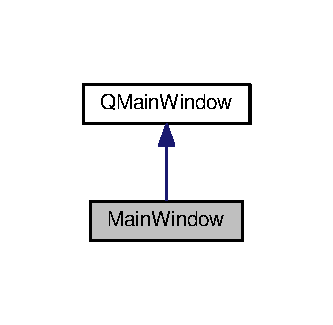
\includegraphics[width=160pt]{classGUI_1_1MainWindow__inherit__graph}
\end{center}
\end{figure}
\subsection*{Public Member Functions}
\begin{DoxyCompactItemize}
\item 
\hyperlink{classGUI_1_1MainWindow_aafaf72c52e0a059620d80026737865b4}{Main\+Window} (\hyperlink{classGUI_1_1QWidget}{G\+U\+I\+::\+Q\+Widget} $\ast$parent)
\item 
\hyperlink{classMemento_1_1MainWindowMemento}{Memento\+::\+Main\+Window\+Memento} \hyperlink{classGUI_1_1MainWindow_ae085d92d1c5bec057a813bd86bc20fa4}{get\+Memento} ()
\item 
void \hyperlink{classGUI_1_1MainWindow_a72db05f1394dbeeb2a76b74d8f65917b}{restore} (\hyperlink{classMemento_1_1MainWindowMemento}{Memento\+::\+Main\+Window\+Memento} memento)
\item 
\hyperlink{classModel_1_1Project}{Model\+::\+Project} \& \hyperlink{classGUI_1_1MainWindow_a0e9fe41bc141b89f4955329b959310eb}{get\+Project} ()
\end{DoxyCompactItemize}
\subsection*{Data Fields}
\begin{DoxyCompactItemize}
\item 
\hyperlink{classModel_1_1Project}{Model\+::\+Project} $\ast$ \hyperlink{classGUI_1_1MainWindow_a870e96d05ee2e8c616461952d01ac408}{loaded\+Project}
\end{DoxyCompactItemize}
\subsection*{Private Member Functions}
\begin{DoxyCompactItemize}
\item 
void \hyperlink{classGUI_1_1MainWindow_ae128dfd6fbafee0370f9912e4112f054}{new\+Project} ()
\item 
void \hyperlink{classGUI_1_1MainWindow_a0e1e7804a53f6d62efc72c9bdbec8571}{undo} ()
\item 
void \hyperlink{classGUI_1_1MainWindow_a65005f9a81d8c7396e2583a80a1f70bf}{save\+As} ()
\item 
void \hyperlink{classGUI_1_1MainWindow_adb575720306afca2c0e0c5930467321b}{load\+Project} ()
\item 
void \hyperlink{classGUI_1_1MainWindow_a5de2650de39370a5fe89f8d918966276}{save\+Project} ()
\item 
void \hyperlink{classGUI_1_1MainWindow_a93c48d6ed036e1a381be53ac67643284}{redo} ()
\item 
void \hyperlink{classGUI_1_1MainWindow_aa72182c9a958af0e87b65ab7bdba0035}{create\+Ui} ()
\item 
void \hyperlink{classGUI_1_1MainWindow_ac3ca31ff0047daecf8bbe393a15e940c}{connect\+Actions} ()
\item 
void \hyperlink{classGUI_1_1MainWindow_a5421da114e56e8856aa455426c24f805}{create\+Menu\+Bar} ()
\end{DoxyCompactItemize}
\subsection*{Private Attributes}
\begin{DoxyCompactItemize}
\item 
Q\+Status\+Bar $\ast$ \hyperlink{classGUI_1_1MainWindow_ab12bbb712331d72b3972876494b01d43}{statusbar}
\item 
Q\+Menu\+Bar $\ast$ \hyperlink{classGUI_1_1MainWindow_a3a7fd0d9d9fcaf5f23b620ecc1d868a2}{menubar\+\_\+project}
\item 
Q\+Menu\+Bar $\ast$ \hyperlink{classGUI_1_1MainWindow_a5beda12aa8191deaad381531b99992f8}{menubar\+\_\+edit}
\item 
Q\+Action $\ast$ \hyperlink{classGUI_1_1MainWindow_a5cf13e75b97a8a55f79a7f1a5dfeccdd}{action\+\_\+new\+Project}
\item 
Q\+Action $\ast$ \hyperlink{classGUI_1_1MainWindow_af4ed54c2c44d393a4c854ca626103f72}{action\+\_\+undo}
\item 
Q\+Action $\ast$ \hyperlink{classGUI_1_1MainWindow_a477f9c21e430c9db3664df4ac4a5bec9}{action\+\_\+save\+As}
\item 
Q\+Action $\ast$ \hyperlink{classGUI_1_1MainWindow_acbc3dfeebc15f93a7808e5a1d7a44492}{action\+\_\+load\+Project}
\item 
Q\+Action $\ast$ \hyperlink{classGUI_1_1MainWindow_a84cc9a3cf59e2fdd3196da97a5faa717}{action\+\_\+save\+Project}
\item 
Q\+Action $\ast$ \hyperlink{classGUI_1_1MainWindow_a76bce8131d4330008b0f40cf8e8b97d6}{action\+\_\+redo}
\item 
Q\+Tab\+Widget $\ast$ \hyperlink{classGUI_1_1MainWindow_aaeb8f9f47ba45615e767b2a7f7b009d9}{tab\+\_\+tabs}
\end{DoxyCompactItemize}


\subsection{Detailed Description}
This class is the main window that is shown. 

\subsection{Constructor \& Destructor Documentation}
\hypertarget{classGUI_1_1MainWindow_aafaf72c52e0a059620d80026737865b4}{}\index{G\+U\+I\+::\+Main\+Window@{G\+U\+I\+::\+Main\+Window}!Main\+Window@{Main\+Window}}
\index{Main\+Window@{Main\+Window}!G\+U\+I\+::\+Main\+Window@{G\+U\+I\+::\+Main\+Window}}
\subsubsection[{Main\+Window}]{\setlength{\rightskip}{0pt plus 5cm}{\bf Main\+Window} (
\begin{DoxyParamCaption}
\item[{{\bf G\+U\+I\+::\+Q\+Widget} $\ast$}]{parent}
\end{DoxyParamCaption}
)}\label{classGUI_1_1MainWindow_aafaf72c52e0a059620d80026737865b4}


Constructor. 



\subsection{Member Function Documentation}
\hypertarget{classGUI_1_1MainWindow_ac3ca31ff0047daecf8bbe393a15e940c}{}\index{G\+U\+I\+::\+Main\+Window@{G\+U\+I\+::\+Main\+Window}!connect\+Actions@{connect\+Actions}}
\index{connect\+Actions@{connect\+Actions}!G\+U\+I\+::\+Main\+Window@{G\+U\+I\+::\+Main\+Window}}
\subsubsection[{connect\+Actions}]{\setlength{\rightskip}{0pt plus 5cm}void connect\+Actions (
\begin{DoxyParamCaption}
{}
\end{DoxyParamCaption}
)\hspace{0.3cm}{\ttfamily [private]}}\label{classGUI_1_1MainWindow_ac3ca31ff0047daecf8bbe393a15e940c}


connect actions in the menu\+Bars to the slots in this class 

\hypertarget{classGUI_1_1MainWindow_a5421da114e56e8856aa455426c24f805}{}\index{G\+U\+I\+::\+Main\+Window@{G\+U\+I\+::\+Main\+Window}!create\+Menu\+Bar@{create\+Menu\+Bar}}
\index{create\+Menu\+Bar@{create\+Menu\+Bar}!G\+U\+I\+::\+Main\+Window@{G\+U\+I\+::\+Main\+Window}}
\subsubsection[{create\+Menu\+Bar}]{\setlength{\rightskip}{0pt plus 5cm}void create\+Menu\+Bar (
\begin{DoxyParamCaption}
{}
\end{DoxyParamCaption}
)\hspace{0.3cm}{\ttfamily [private]}}\label{classGUI_1_1MainWindow_a5421da114e56e8856aa455426c24f805}
\hypertarget{classGUI_1_1MainWindow_aa72182c9a958af0e87b65ab7bdba0035}{}\index{G\+U\+I\+::\+Main\+Window@{G\+U\+I\+::\+Main\+Window}!create\+Ui@{create\+Ui}}
\index{create\+Ui@{create\+Ui}!G\+U\+I\+::\+Main\+Window@{G\+U\+I\+::\+Main\+Window}}
\subsubsection[{create\+Ui}]{\setlength{\rightskip}{0pt plus 5cm}void create\+Ui (
\begin{DoxyParamCaption}
{}
\end{DoxyParamCaption}
)\hspace{0.3cm}{\ttfamily [private]}}\label{classGUI_1_1MainWindow_aa72182c9a958af0e87b65ab7bdba0035}


creates the U\+I 

\hypertarget{classGUI_1_1MainWindow_ae085d92d1c5bec057a813bd86bc20fa4}{}\index{G\+U\+I\+::\+Main\+Window@{G\+U\+I\+::\+Main\+Window}!get\+Memento@{get\+Memento}}
\index{get\+Memento@{get\+Memento}!G\+U\+I\+::\+Main\+Window@{G\+U\+I\+::\+Main\+Window}}
\subsubsection[{get\+Memento}]{\setlength{\rightskip}{0pt plus 5cm}{\bf Memento\+::\+Main\+Window\+Memento} get\+Memento (
\begin{DoxyParamCaption}
{}
\end{DoxyParamCaption}
)}\label{classGUI_1_1MainWindow_ae085d92d1c5bec057a813bd86bc20fa4}


Creates a memento which contains the state of the window. 

\begin{DoxyReturn}{Returns}
The created memento.
\end{DoxyReturn}
\hypertarget{classGUI_1_1MainWindow_a0e9fe41bc141b89f4955329b959310eb}{}\index{G\+U\+I\+::\+Main\+Window@{G\+U\+I\+::\+Main\+Window}!get\+Project@{get\+Project}}
\index{get\+Project@{get\+Project}!G\+U\+I\+::\+Main\+Window@{G\+U\+I\+::\+Main\+Window}}
\subsubsection[{get\+Project}]{\setlength{\rightskip}{0pt plus 5cm}{\bf Model\+::\+Project} \& get\+Project (
\begin{DoxyParamCaption}
{}
\end{DoxyParamCaption}
)}\label{classGUI_1_1MainWindow_a0e9fe41bc141b89f4955329b959310eb}


Returns the project that is currently loaded. 

\begin{DoxyReturn}{Returns}
The currently loaded project.
\end{DoxyReturn}
\hypertarget{classGUI_1_1MainWindow_adb575720306afca2c0e0c5930467321b}{}\index{G\+U\+I\+::\+Main\+Window@{G\+U\+I\+::\+Main\+Window}!load\+Project@{load\+Project}}
\index{load\+Project@{load\+Project}!G\+U\+I\+::\+Main\+Window@{G\+U\+I\+::\+Main\+Window}}
\subsubsection[{load\+Project}]{\setlength{\rightskip}{0pt plus 5cm}void load\+Project (
\begin{DoxyParamCaption}
{}
\end{DoxyParamCaption}
)\hspace{0.3cm}{\ttfamily [private]}}\label{classGUI_1_1MainWindow_adb575720306afca2c0e0c5930467321b}


Slot\+:connected with action\+\_\+load\+Project.\+triggered() opens Q\+File\+Dialog and opens project in the selected file if possible 

\hypertarget{classGUI_1_1MainWindow_ae128dfd6fbafee0370f9912e4112f054}{}\index{G\+U\+I\+::\+Main\+Window@{G\+U\+I\+::\+Main\+Window}!new\+Project@{new\+Project}}
\index{new\+Project@{new\+Project}!G\+U\+I\+::\+Main\+Window@{G\+U\+I\+::\+Main\+Window}}
\subsubsection[{new\+Project}]{\setlength{\rightskip}{0pt plus 5cm}void new\+Project (
\begin{DoxyParamCaption}
{}
\end{DoxyParamCaption}
)\hspace{0.3cm}{\ttfamily [private]}}\label{classGUI_1_1MainWindow_ae128dfd6fbafee0370f9912e4112f054}


slot creates new project, removes existing one 

\hypertarget{classGUI_1_1MainWindow_a93c48d6ed036e1a381be53ac67643284}{}\index{G\+U\+I\+::\+Main\+Window@{G\+U\+I\+::\+Main\+Window}!redo@{redo}}
\index{redo@{redo}!G\+U\+I\+::\+Main\+Window@{G\+U\+I\+::\+Main\+Window}}
\subsubsection[{redo}]{\setlength{\rightskip}{0pt plus 5cm}void redo (
\begin{DoxyParamCaption}
{}
\end{DoxyParamCaption}
)\hspace{0.3cm}{\ttfamily [private]}}\label{classGUI_1_1MainWindow_a93c48d6ed036e1a381be53ac67643284}


Slot\+:connected with action\+\_\+redo.\+triggered() redo action if undo has been used 

\hypertarget{classGUI_1_1MainWindow_a72db05f1394dbeeb2a76b74d8f65917b}{}\index{G\+U\+I\+::\+Main\+Window@{G\+U\+I\+::\+Main\+Window}!restore@{restore}}
\index{restore@{restore}!G\+U\+I\+::\+Main\+Window@{G\+U\+I\+::\+Main\+Window}}
\subsubsection[{restore}]{\setlength{\rightskip}{0pt plus 5cm}void restore (
\begin{DoxyParamCaption}
\item[{{\bf Memento\+::\+Main\+Window\+Memento}}]{memento}
\end{DoxyParamCaption}
)}\label{classGUI_1_1MainWindow_a72db05f1394dbeeb2a76b74d8f65917b}


Restores the window based on the memento. 


\begin{DoxyParams}{Parameters}
{\em memento} & The memento which contains the state of the window.\\
\hline
\end{DoxyParams}
\hypertarget{classGUI_1_1MainWindow_a65005f9a81d8c7396e2583a80a1f70bf}{}\index{G\+U\+I\+::\+Main\+Window@{G\+U\+I\+::\+Main\+Window}!save\+As@{save\+As}}
\index{save\+As@{save\+As}!G\+U\+I\+::\+Main\+Window@{G\+U\+I\+::\+Main\+Window}}
\subsubsection[{save\+As}]{\setlength{\rightskip}{0pt plus 5cm}void save\+As (
\begin{DoxyParamCaption}
{}
\end{DoxyParamCaption}
)\hspace{0.3cm}{\ttfamily [private]}}\label{classGUI_1_1MainWindow_a65005f9a81d8c7396e2583a80a1f70bf}


Slot\+:connected with action\+\_\+save\+As.\+triggered() Opens Q\+File\+Dialog and saves project in selected file 

\hypertarget{classGUI_1_1MainWindow_a5de2650de39370a5fe89f8d918966276}{}\index{G\+U\+I\+::\+Main\+Window@{G\+U\+I\+::\+Main\+Window}!save\+Project@{save\+Project}}
\index{save\+Project@{save\+Project}!G\+U\+I\+::\+Main\+Window@{G\+U\+I\+::\+Main\+Window}}
\subsubsection[{save\+Project}]{\setlength{\rightskip}{0pt plus 5cm}void save\+Project (
\begin{DoxyParamCaption}
{}
\end{DoxyParamCaption}
)\hspace{0.3cm}{\ttfamily [private]}}\label{classGUI_1_1MainWindow_a5de2650de39370a5fe89f8d918966276}


Slot\+:connected with action\+\_\+save\+Project.\+triggered() opens Q\+File\+Dialog and saves project in selected file 

\hypertarget{classGUI_1_1MainWindow_a0e1e7804a53f6d62efc72c9bdbec8571}{}\index{G\+U\+I\+::\+Main\+Window@{G\+U\+I\+::\+Main\+Window}!undo@{undo}}
\index{undo@{undo}!G\+U\+I\+::\+Main\+Window@{G\+U\+I\+::\+Main\+Window}}
\subsubsection[{undo}]{\setlength{\rightskip}{0pt plus 5cm}void undo (
\begin{DoxyParamCaption}
{}
\end{DoxyParamCaption}
)\hspace{0.3cm}{\ttfamily [private]}}\label{classGUI_1_1MainWindow_a0e1e7804a53f6d62efc72c9bdbec8571}


Slot\+:connected with action\+\_\+undo.\+triggered() undo last action if possible 



\subsection{Field Documentation}
\hypertarget{classGUI_1_1MainWindow_acbc3dfeebc15f93a7808e5a1d7a44492}{}\index{G\+U\+I\+::\+Main\+Window@{G\+U\+I\+::\+Main\+Window}!action\+\_\+load\+Project@{action\+\_\+load\+Project}}
\index{action\+\_\+load\+Project@{action\+\_\+load\+Project}!G\+U\+I\+::\+Main\+Window@{G\+U\+I\+::\+Main\+Window}}
\subsubsection[{action\+\_\+load\+Project}]{\setlength{\rightskip}{0pt plus 5cm}Q\+Action$\ast$ action\+\_\+load\+Project\hspace{0.3cm}{\ttfamily [private]}}\label{classGUI_1_1MainWindow_acbc3dfeebc15f93a7808e5a1d7a44492}
\hypertarget{classGUI_1_1MainWindow_a5cf13e75b97a8a55f79a7f1a5dfeccdd}{}\index{G\+U\+I\+::\+Main\+Window@{G\+U\+I\+::\+Main\+Window}!action\+\_\+new\+Project@{action\+\_\+new\+Project}}
\index{action\+\_\+new\+Project@{action\+\_\+new\+Project}!G\+U\+I\+::\+Main\+Window@{G\+U\+I\+::\+Main\+Window}}
\subsubsection[{action\+\_\+new\+Project}]{\setlength{\rightskip}{0pt plus 5cm}Q\+Action$\ast$ action\+\_\+new\+Project\hspace{0.3cm}{\ttfamily [private]}}\label{classGUI_1_1MainWindow_a5cf13e75b97a8a55f79a7f1a5dfeccdd}
\hypertarget{classGUI_1_1MainWindow_a76bce8131d4330008b0f40cf8e8b97d6}{}\index{G\+U\+I\+::\+Main\+Window@{G\+U\+I\+::\+Main\+Window}!action\+\_\+redo@{action\+\_\+redo}}
\index{action\+\_\+redo@{action\+\_\+redo}!G\+U\+I\+::\+Main\+Window@{G\+U\+I\+::\+Main\+Window}}
\subsubsection[{action\+\_\+redo}]{\setlength{\rightskip}{0pt plus 5cm}Q\+Action$\ast$ action\+\_\+redo\hspace{0.3cm}{\ttfamily [private]}}\label{classGUI_1_1MainWindow_a76bce8131d4330008b0f40cf8e8b97d6}
\hypertarget{classGUI_1_1MainWindow_a477f9c21e430c9db3664df4ac4a5bec9}{}\index{G\+U\+I\+::\+Main\+Window@{G\+U\+I\+::\+Main\+Window}!action\+\_\+save\+As@{action\+\_\+save\+As}}
\index{action\+\_\+save\+As@{action\+\_\+save\+As}!G\+U\+I\+::\+Main\+Window@{G\+U\+I\+::\+Main\+Window}}
\subsubsection[{action\+\_\+save\+As}]{\setlength{\rightskip}{0pt plus 5cm}Q\+Action$\ast$ action\+\_\+save\+As\hspace{0.3cm}{\ttfamily [private]}}\label{classGUI_1_1MainWindow_a477f9c21e430c9db3664df4ac4a5bec9}
\hypertarget{classGUI_1_1MainWindow_a84cc9a3cf59e2fdd3196da97a5faa717}{}\index{G\+U\+I\+::\+Main\+Window@{G\+U\+I\+::\+Main\+Window}!action\+\_\+save\+Project@{action\+\_\+save\+Project}}
\index{action\+\_\+save\+Project@{action\+\_\+save\+Project}!G\+U\+I\+::\+Main\+Window@{G\+U\+I\+::\+Main\+Window}}
\subsubsection[{action\+\_\+save\+Project}]{\setlength{\rightskip}{0pt plus 5cm}Q\+Action$\ast$ action\+\_\+save\+Project\hspace{0.3cm}{\ttfamily [private]}}\label{classGUI_1_1MainWindow_a84cc9a3cf59e2fdd3196da97a5faa717}
\hypertarget{classGUI_1_1MainWindow_af4ed54c2c44d393a4c854ca626103f72}{}\index{G\+U\+I\+::\+Main\+Window@{G\+U\+I\+::\+Main\+Window}!action\+\_\+undo@{action\+\_\+undo}}
\index{action\+\_\+undo@{action\+\_\+undo}!G\+U\+I\+::\+Main\+Window@{G\+U\+I\+::\+Main\+Window}}
\subsubsection[{action\+\_\+undo}]{\setlength{\rightskip}{0pt plus 5cm}Q\+Action$\ast$ action\+\_\+undo\hspace{0.3cm}{\ttfamily [private]}}\label{classGUI_1_1MainWindow_af4ed54c2c44d393a4c854ca626103f72}
\hypertarget{classGUI_1_1MainWindow_a870e96d05ee2e8c616461952d01ac408}{}\index{G\+U\+I\+::\+Main\+Window@{G\+U\+I\+::\+Main\+Window}!loaded\+Project@{loaded\+Project}}
\index{loaded\+Project@{loaded\+Project}!G\+U\+I\+::\+Main\+Window@{G\+U\+I\+::\+Main\+Window}}
\subsubsection[{loaded\+Project}]{\setlength{\rightskip}{0pt plus 5cm}{\bf Model\+::\+Project}$\ast$ loaded\+Project}\label{classGUI_1_1MainWindow_a870e96d05ee2e8c616461952d01ac408}
\hypertarget{classGUI_1_1MainWindow_a5beda12aa8191deaad381531b99992f8}{}\index{G\+U\+I\+::\+Main\+Window@{G\+U\+I\+::\+Main\+Window}!menubar\+\_\+edit@{menubar\+\_\+edit}}
\index{menubar\+\_\+edit@{menubar\+\_\+edit}!G\+U\+I\+::\+Main\+Window@{G\+U\+I\+::\+Main\+Window}}
\subsubsection[{menubar\+\_\+edit}]{\setlength{\rightskip}{0pt plus 5cm}Q\+Menu\+Bar$\ast$ menubar\+\_\+edit\hspace{0.3cm}{\ttfamily [private]}}\label{classGUI_1_1MainWindow_a5beda12aa8191deaad381531b99992f8}
\hypertarget{classGUI_1_1MainWindow_a3a7fd0d9d9fcaf5f23b620ecc1d868a2}{}\index{G\+U\+I\+::\+Main\+Window@{G\+U\+I\+::\+Main\+Window}!menubar\+\_\+project@{menubar\+\_\+project}}
\index{menubar\+\_\+project@{menubar\+\_\+project}!G\+U\+I\+::\+Main\+Window@{G\+U\+I\+::\+Main\+Window}}
\subsubsection[{menubar\+\_\+project}]{\setlength{\rightskip}{0pt plus 5cm}Q\+Menu\+Bar$\ast$ menubar\+\_\+project\hspace{0.3cm}{\ttfamily [private]}}\label{classGUI_1_1MainWindow_a3a7fd0d9d9fcaf5f23b620ecc1d868a2}
\hypertarget{classGUI_1_1MainWindow_ab12bbb712331d72b3972876494b01d43}{}\index{G\+U\+I\+::\+Main\+Window@{G\+U\+I\+::\+Main\+Window}!statusbar@{statusbar}}
\index{statusbar@{statusbar}!G\+U\+I\+::\+Main\+Window@{G\+U\+I\+::\+Main\+Window}}
\subsubsection[{statusbar}]{\setlength{\rightskip}{0pt plus 5cm}Q\+Status\+Bar$\ast$ statusbar\hspace{0.3cm}{\ttfamily [private]}}\label{classGUI_1_1MainWindow_ab12bbb712331d72b3972876494b01d43}
\hypertarget{classGUI_1_1MainWindow_aaeb8f9f47ba45615e767b2a7f7b009d9}{}\index{G\+U\+I\+::\+Main\+Window@{G\+U\+I\+::\+Main\+Window}!tab\+\_\+tabs@{tab\+\_\+tabs}}
\index{tab\+\_\+tabs@{tab\+\_\+tabs}!G\+U\+I\+::\+Main\+Window@{G\+U\+I\+::\+Main\+Window}}
\subsubsection[{tab\+\_\+tabs}]{\setlength{\rightskip}{0pt plus 5cm}Q\+Tab\+Widget$\ast$ tab\+\_\+tabs\hspace{0.3cm}{\ttfamily [private]}}\label{classGUI_1_1MainWindow_aaeb8f9f47ba45615e767b2a7f7b009d9}

\hypertarget{classMemento_1_1MainWindowMemento}{}\section{Main\+Window\+Memento Class Reference}
\label{classMemento_1_1MainWindowMemento}\index{Main\+Window\+Memento@{Main\+Window\+Memento}}
\subsection*{Public Member Functions}
\begin{DoxyCompactItemize}
\item 
\hyperlink{classMemento_1_1MainWindowMemento_a2ce9d23f57fc6397812a080c3111d56c}{Main\+Window\+Memento} ()
\item 
int \hyperlink{classMemento_1_1MainWindowMemento_a876003270f9665415d49783d0669511a}{get\+Selected\+Tab} ()
\item 
void \hyperlink{classMemento_1_1MainWindowMemento_a9ec6af835d6fdbf10eb8a6db5ad59578}{set\+Selected\+Tab} (int \hyperlink{classMemento_1_1MainWindowMemento_aa1aed58bddd5b90f62a2516015ab3c04}{selected\+Tab})
\item 
\hyperlink{classMemento_1_1AnalysisTabMemento}{Memento\+::\+Analysis\+Tab\+Memento} \hyperlink{classMemento_1_1MainWindowMemento_aeaae363ca3c1aaa02d9acd9fbcd669e5}{get\+Analysis\+Tab\+Memento} ()
\item 
void \hyperlink{classMemento_1_1MainWindowMemento_a2f3cbb73b8364dfb6640b0e5225600cf}{set\+Analysis\+Tab\+Memento} (\hyperlink{classMemento_1_1AnalysisTabMemento}{Memento\+::\+Analysis\+Tab\+Memento} analysis\+Tab\+Me\+Mento)
\item 
\hyperlink{classMemento_1_1FilterTabMemento}{Memento\+::\+Filter\+Tab\+Memento} \hyperlink{classMemento_1_1MainWindowMemento_aca564eecb180bc19d899b14c9ebe5486}{get\+Filter\+Tab\+Memento} ()
\item 
void \hyperlink{classMemento_1_1MainWindowMemento_aabc5961524bfb567d2f7f5bdf79e6661}{set\+Filter\+Tab\+Memento} (\hyperlink{classMemento_1_1FilterTabMemento}{Memento\+::\+Filter\+Tab\+Memento} filter\+Tab\+Memento)
\end{DoxyCompactItemize}
\subsection*{Private Attributes}
\begin{DoxyCompactItemize}
\item 
int \hyperlink{classMemento_1_1MainWindowMemento_aa1aed58bddd5b90f62a2516015ab3c04}{selected\+Tab}
\item 
\hyperlink{classMemento_1_1AnalysisTabMemento}{Memento\+::\+Analysis\+Tab\+Memento} $\ast$ \hyperlink{classMemento_1_1MainWindowMemento_a706b928eccc0de3d1175f53e3bf6e391}{analysis\+Tab}
\item 
\hyperlink{classMemento_1_1FilterTabMemento}{Memento\+::\+Filter\+Tab\+Memento} $\ast$ \hyperlink{classMemento_1_1MainWindowMemento_aa834b7b9b12f3913750cd558db4b7796}{filter\+Tab}
\end{DoxyCompactItemize}


\subsection{Detailed Description}
This class is the memento for the Main\+Window. 

\subsection{Constructor \& Destructor Documentation}
\hypertarget{classMemento_1_1MainWindowMemento_a2ce9d23f57fc6397812a080c3111d56c}{}\index{Memento\+::\+Main\+Window\+Memento@{Memento\+::\+Main\+Window\+Memento}!Main\+Window\+Memento@{Main\+Window\+Memento}}
\index{Main\+Window\+Memento@{Main\+Window\+Memento}!Memento\+::\+Main\+Window\+Memento@{Memento\+::\+Main\+Window\+Memento}}
\subsubsection[{Main\+Window\+Memento}]{\setlength{\rightskip}{0pt plus 5cm}{\bf Main\+Window\+Memento} (
\begin{DoxyParamCaption}
{}
\end{DoxyParamCaption}
)}\label{classMemento_1_1MainWindowMemento_a2ce9d23f57fc6397812a080c3111d56c}


Constructor. 



\subsection{Member Function Documentation}
\hypertarget{classMemento_1_1MainWindowMemento_aeaae363ca3c1aaa02d9acd9fbcd669e5}{}\index{Memento\+::\+Main\+Window\+Memento@{Memento\+::\+Main\+Window\+Memento}!get\+Analysis\+Tab\+Memento@{get\+Analysis\+Tab\+Memento}}
\index{get\+Analysis\+Tab\+Memento@{get\+Analysis\+Tab\+Memento}!Memento\+::\+Main\+Window\+Memento@{Memento\+::\+Main\+Window\+Memento}}
\subsubsection[{get\+Analysis\+Tab\+Memento}]{\setlength{\rightskip}{0pt plus 5cm}{\bf Memento\+::\+Analysis\+Tab\+Memento} get\+Analysis\+Tab\+Memento (
\begin{DoxyParamCaption}
{}
\end{DoxyParamCaption}
)}\label{classMemento_1_1MainWindowMemento_aeaae363ca3c1aaa02d9acd9fbcd669e5}


Returns the \hyperlink{classMemento_1_1AnalysisTabMemento}{Analysis\+Tab\+Memento}. 

\begin{DoxyReturn}{Returns}
The \hyperlink{classMemento_1_1AnalysisTabMemento}{Analysis\+Tab\+Memento}.
\end{DoxyReturn}
\hypertarget{classMemento_1_1MainWindowMemento_aca564eecb180bc19d899b14c9ebe5486}{}\index{Memento\+::\+Main\+Window\+Memento@{Memento\+::\+Main\+Window\+Memento}!get\+Filter\+Tab\+Memento@{get\+Filter\+Tab\+Memento}}
\index{get\+Filter\+Tab\+Memento@{get\+Filter\+Tab\+Memento}!Memento\+::\+Main\+Window\+Memento@{Memento\+::\+Main\+Window\+Memento}}
\subsubsection[{get\+Filter\+Tab\+Memento}]{\setlength{\rightskip}{0pt plus 5cm}{\bf Memento\+::\+Filter\+Tab\+Memento} get\+Filter\+Tab\+Memento (
\begin{DoxyParamCaption}
{}
\end{DoxyParamCaption}
)}\label{classMemento_1_1MainWindowMemento_aca564eecb180bc19d899b14c9ebe5486}


Returns the \hyperlink{classMemento_1_1FilterTabMemento}{Filter\+Tab\+Memento}. 

\begin{DoxyReturn}{Returns}
The \hyperlink{classMemento_1_1FilterTabMemento}{Filter\+Tab\+Memento}.
\end{DoxyReturn}
\hypertarget{classMemento_1_1MainWindowMemento_a876003270f9665415d49783d0669511a}{}\index{Memento\+::\+Main\+Window\+Memento@{Memento\+::\+Main\+Window\+Memento}!get\+Selected\+Tab@{get\+Selected\+Tab}}
\index{get\+Selected\+Tab@{get\+Selected\+Tab}!Memento\+::\+Main\+Window\+Memento@{Memento\+::\+Main\+Window\+Memento}}
\subsubsection[{get\+Selected\+Tab}]{\setlength{\rightskip}{0pt plus 5cm}int get\+Selected\+Tab (
\begin{DoxyParamCaption}
{}
\end{DoxyParamCaption}
)}\label{classMemento_1_1MainWindowMemento_a876003270f9665415d49783d0669511a}


Returns the currently selected tab. 

\begin{DoxyReturn}{Returns}
The currently selected tab.
\end{DoxyReturn}
\hypertarget{classMemento_1_1MainWindowMemento_a2f3cbb73b8364dfb6640b0e5225600cf}{}\index{Memento\+::\+Main\+Window\+Memento@{Memento\+::\+Main\+Window\+Memento}!set\+Analysis\+Tab\+Memento@{set\+Analysis\+Tab\+Memento}}
\index{set\+Analysis\+Tab\+Memento@{set\+Analysis\+Tab\+Memento}!Memento\+::\+Main\+Window\+Memento@{Memento\+::\+Main\+Window\+Memento}}
\subsubsection[{set\+Analysis\+Tab\+Memento}]{\setlength{\rightskip}{0pt plus 5cm}void set\+Analysis\+Tab\+Memento (
\begin{DoxyParamCaption}
\item[{{\bf Memento\+::\+Analysis\+Tab\+Memento}}]{analysis\+Tab\+Me\+Mento}
\end{DoxyParamCaption}
)}\label{classMemento_1_1MainWindowMemento_a2f3cbb73b8364dfb6640b0e5225600cf}


Sets the \hyperlink{classMemento_1_1AnalysisTabMemento}{Analysis\+Tab\+Memento}. 


\begin{DoxyParams}{Parameters}
{\em analysis\+Tab\+Me\+Mento} & The \hyperlink{classMemento_1_1AnalysisTabMemento}{Analysis\+Tab\+Memento}.\\
\hline
\end{DoxyParams}
\hypertarget{classMemento_1_1MainWindowMemento_aabc5961524bfb567d2f7f5bdf79e6661}{}\index{Memento\+::\+Main\+Window\+Memento@{Memento\+::\+Main\+Window\+Memento}!set\+Filter\+Tab\+Memento@{set\+Filter\+Tab\+Memento}}
\index{set\+Filter\+Tab\+Memento@{set\+Filter\+Tab\+Memento}!Memento\+::\+Main\+Window\+Memento@{Memento\+::\+Main\+Window\+Memento}}
\subsubsection[{set\+Filter\+Tab\+Memento}]{\setlength{\rightskip}{0pt plus 5cm}void set\+Filter\+Tab\+Memento (
\begin{DoxyParamCaption}
\item[{{\bf Memento\+::\+Filter\+Tab\+Memento}}]{filter\+Tab\+Memento}
\end{DoxyParamCaption}
)}\label{classMemento_1_1MainWindowMemento_aabc5961524bfb567d2f7f5bdf79e6661}


Sets the \hyperlink{classMemento_1_1FilterTabMemento}{Filter\+Tab\+Memento}. 


\begin{DoxyParams}{Parameters}
{\em filter\+Tab\+Memento} & The \hyperlink{classMemento_1_1FilterTabMemento}{Filter\+Tab\+Memento}.\\
\hline
\end{DoxyParams}
\hypertarget{classMemento_1_1MainWindowMemento_a9ec6af835d6fdbf10eb8a6db5ad59578}{}\index{Memento\+::\+Main\+Window\+Memento@{Memento\+::\+Main\+Window\+Memento}!set\+Selected\+Tab@{set\+Selected\+Tab}}
\index{set\+Selected\+Tab@{set\+Selected\+Tab}!Memento\+::\+Main\+Window\+Memento@{Memento\+::\+Main\+Window\+Memento}}
\subsubsection[{set\+Selected\+Tab}]{\setlength{\rightskip}{0pt plus 5cm}void set\+Selected\+Tab (
\begin{DoxyParamCaption}
\item[{int}]{selected\+Tab}
\end{DoxyParamCaption}
)}\label{classMemento_1_1MainWindowMemento_a9ec6af835d6fdbf10eb8a6db5ad59578}


Sets the currently selected tab. 


\begin{DoxyParams}{Parameters}
{\em selected\+Tab} & The currently selected tab.\\
\hline
\end{DoxyParams}


\subsection{Field Documentation}
\hypertarget{classMemento_1_1MainWindowMemento_a706b928eccc0de3d1175f53e3bf6e391}{}\index{Memento\+::\+Main\+Window\+Memento@{Memento\+::\+Main\+Window\+Memento}!analysis\+Tab@{analysis\+Tab}}
\index{analysis\+Tab@{analysis\+Tab}!Memento\+::\+Main\+Window\+Memento@{Memento\+::\+Main\+Window\+Memento}}
\subsubsection[{analysis\+Tab}]{\setlength{\rightskip}{0pt plus 5cm}{\bf Memento\+::\+Analysis\+Tab\+Memento}$\ast$ analysis\+Tab\hspace{0.3cm}{\ttfamily [private]}}\label{classMemento_1_1MainWindowMemento_a706b928eccc0de3d1175f53e3bf6e391}
\hypertarget{classMemento_1_1MainWindowMemento_aa834b7b9b12f3913750cd558db4b7796}{}\index{Memento\+::\+Main\+Window\+Memento@{Memento\+::\+Main\+Window\+Memento}!filter\+Tab@{filter\+Tab}}
\index{filter\+Tab@{filter\+Tab}!Memento\+::\+Main\+Window\+Memento@{Memento\+::\+Main\+Window\+Memento}}
\subsubsection[{filter\+Tab}]{\setlength{\rightskip}{0pt plus 5cm}{\bf Memento\+::\+Filter\+Tab\+Memento}$\ast$ filter\+Tab\hspace{0.3cm}{\ttfamily [private]}}\label{classMemento_1_1MainWindowMemento_aa834b7b9b12f3913750cd558db4b7796}
\hypertarget{classMemento_1_1MainWindowMemento_aa1aed58bddd5b90f62a2516015ab3c04}{}\index{Memento\+::\+Main\+Window\+Memento@{Memento\+::\+Main\+Window\+Memento}!selected\+Tab@{selected\+Tab}}
\index{selected\+Tab@{selected\+Tab}!Memento\+::\+Main\+Window\+Memento@{Memento\+::\+Main\+Window\+Memento}}
\subsubsection[{selected\+Tab}]{\setlength{\rightskip}{0pt plus 5cm}int selected\+Tab\hspace{0.3cm}{\ttfamily [private]}}\label{classMemento_1_1MainWindowMemento_aa1aed58bddd5b90f62a2516015ab3c04}

\hypertarget{classModel_1_1Filter_1_1MirrorFilter}{}\section{Mirror\+Filter Class Reference}
\label{classModel_1_1Filter_1_1MirrorFilter}\index{Mirror\+Filter@{Mirror\+Filter}}
\subsection*{Public Member Functions}
\begin{DoxyCompactItemize}
\item 
\hyperlink{classModel_1_1Filter_1_1MirrorFilter_a534aebee3440f56936f691affb8be0d5}{Mirror\+Filter} ()
\item 
string \hyperlink{classModel_1_1Filter_1_1MirrorFilter_a62b7b60e24f92234393b840b35808e06}{get\+Filter\+Description} ()
\item 
string \hyperlink{classModel_1_1Filter_1_1MirrorFilter_a11335e13e50af74108bf926dc1340b4b}{get\+Name} ()
\item 
\hyperlink{namespaceModel_1_1Filter_a8a20195c97d8c704572b5922370c2fbc}{Model\+::\+Filter\+::\+Mirror\+Mode} \hyperlink{classModel_1_1Filter_1_1MirrorFilter_a49ba6d929bc296cb263b4c34b3f90f02}{get\+Mode} ()
\item 
void \hyperlink{classModel_1_1Filter_1_1MirrorFilter_a862e3564f078c1c424e88430eb1b283c}{set\+Mode} (\hyperlink{namespaceModel_1_1Filter_a8a20195c97d8c704572b5922370c2fbc}{Model\+::\+Filter\+::\+Mirror\+Mode} mode)
\end{DoxyCompactItemize}
\subsection*{Additional Inherited Members}


\subsection{Detailed Description}
Mirrors the video horizontally or vertically. 

\subsection{Constructor \& Destructor Documentation}
\hypertarget{classModel_1_1Filter_1_1MirrorFilter_a534aebee3440f56936f691affb8be0d5}{}\index{Model\+::\+Filter\+::\+Mirror\+Filter@{Model\+::\+Filter\+::\+Mirror\+Filter}!Mirror\+Filter@{Mirror\+Filter}}
\index{Mirror\+Filter@{Mirror\+Filter}!Model\+::\+Filter\+::\+Mirror\+Filter@{Model\+::\+Filter\+::\+Mirror\+Filter}}
\subsubsection[{Mirror\+Filter}]{\setlength{\rightskip}{0pt plus 5cm}{\bf Mirror\+Filter} (
\begin{DoxyParamCaption}
{}
\end{DoxyParamCaption}
)}\label{classModel_1_1Filter_1_1MirrorFilter_a534aebee3440f56936f691affb8be0d5}


Constructor. 



\subsection{Member Function Documentation}
\hypertarget{classModel_1_1Filter_1_1MirrorFilter_a62b7b60e24f92234393b840b35808e06}{}\index{Model\+::\+Filter\+::\+Mirror\+Filter@{Model\+::\+Filter\+::\+Mirror\+Filter}!get\+Filter\+Description@{get\+Filter\+Description}}
\index{get\+Filter\+Description@{get\+Filter\+Description}!Model\+::\+Filter\+::\+Mirror\+Filter@{Model\+::\+Filter\+::\+Mirror\+Filter}}
\subsubsection[{get\+Filter\+Description}]{\setlength{\rightskip}{0pt plus 5cm}string get\+Filter\+Description (
\begin{DoxyParamCaption}
{}
\end{DoxyParamCaption}
)\hspace{0.3cm}{\ttfamily [virtual]}}\label{classModel_1_1Filter_1_1MirrorFilter_a62b7b60e24f92234393b840b35808e06}


Returns the string that the ffmpeg library needs to apply the filter to a video. 

\begin{DoxyReturn}{Returns}
The string for the ffmpeg library.
\end{DoxyReturn}


Implements \hyperlink{classModel_1_1Filter_1_1Filter_a453fcafa809afa1ce58d9ef95d5f26c0}{Filter}.

\hypertarget{classModel_1_1Filter_1_1MirrorFilter_a49ba6d929bc296cb263b4c34b3f90f02}{}\index{Model\+::\+Filter\+::\+Mirror\+Filter@{Model\+::\+Filter\+::\+Mirror\+Filter}!get\+Mode@{get\+Mode}}
\index{get\+Mode@{get\+Mode}!Model\+::\+Filter\+::\+Mirror\+Filter@{Model\+::\+Filter\+::\+Mirror\+Filter}}
\subsubsection[{get\+Mode}]{\setlength{\rightskip}{0pt plus 5cm}{\bf Model\+::\+Filter\+::\+Mirror\+Mode} get\+Mode (
\begin{DoxyParamCaption}
{}
\end{DoxyParamCaption}
)}\label{classModel_1_1Filter_1_1MirrorFilter_a49ba6d929bc296cb263b4c34b3f90f02}


Returns the Mirror\+Mode. 

\begin{DoxyReturn}{Returns}
The Mirror\+Mode.
\end{DoxyReturn}
\hypertarget{classModel_1_1Filter_1_1MirrorFilter_a11335e13e50af74108bf926dc1340b4b}{}\index{Model\+::\+Filter\+::\+Mirror\+Filter@{Model\+::\+Filter\+::\+Mirror\+Filter}!get\+Name@{get\+Name}}
\index{get\+Name@{get\+Name}!Model\+::\+Filter\+::\+Mirror\+Filter@{Model\+::\+Filter\+::\+Mirror\+Filter}}
\subsubsection[{get\+Name}]{\setlength{\rightskip}{0pt plus 5cm}string get\+Name (
\begin{DoxyParamCaption}
{}
\end{DoxyParamCaption}
)\hspace{0.3cm}{\ttfamily [virtual]}}\label{classModel_1_1Filter_1_1MirrorFilter_a11335e13e50af74108bf926dc1340b4b}


Returns the name of the filter. 

\begin{DoxyReturn}{Returns}
The filtername.
\end{DoxyReturn}


Implements \hyperlink{classModel_1_1Filter_1_1Filter_ade93aa98c68d185a9c03784d36140225}{Filter}.

\hypertarget{classModel_1_1Filter_1_1MirrorFilter_a862e3564f078c1c424e88430eb1b283c}{}\index{Model\+::\+Filter\+::\+Mirror\+Filter@{Model\+::\+Filter\+::\+Mirror\+Filter}!set\+Mode@{set\+Mode}}
\index{set\+Mode@{set\+Mode}!Model\+::\+Filter\+::\+Mirror\+Filter@{Model\+::\+Filter\+::\+Mirror\+Filter}}
\subsubsection[{set\+Mode}]{\setlength{\rightskip}{0pt plus 5cm}void set\+Mode (
\begin{DoxyParamCaption}
\item[{{\bf Model\+::\+Filter\+::\+Mirror\+Mode}}]{mode}
\end{DoxyParamCaption}
)}\label{classModel_1_1Filter_1_1MirrorFilter_a862e3564f078c1c424e88430eb1b283c}


Sets the Mirror\+Mode. 


\begin{DoxyParams}{Parameters}
{\em mode} & The Mirror\+Mode.\\
\hline
\end{DoxyParams}

\hypertarget{classGUI_1_1MirrorFilterBox}{}\section{Mirror\+Filter\+Box Class Reference}
\label{classGUI_1_1MirrorFilterBox}\index{Mirror\+Filter\+Box@{Mirror\+Filter\+Box}}
\subsection*{Public Member Functions}
\begin{DoxyCompactItemize}
\item 
\hyperlink{classGUI_1_1MirrorFilterBox_a2ca521332b6bba79b0897b1679e8af69}{Mirror\+Filter\+Box} (\hyperlink{classGUI_1_1Player_1_1QWidget}{G\+U\+I\+::\+Player\+::\+Q\+Widget} $\ast$parent)
\end{DoxyCompactItemize}
\subsection*{Additional Inherited Members}


\subsection{Detailed Description}
This class contains the gui elements for changing the options of a mirror filter. 

\subsection{Constructor \& Destructor Documentation}
\hypertarget{classGUI_1_1MirrorFilterBox_a2ca521332b6bba79b0897b1679e8af69}{}\index{G\+U\+I\+::\+Mirror\+Filter\+Box@{G\+U\+I\+::\+Mirror\+Filter\+Box}!Mirror\+Filter\+Box@{Mirror\+Filter\+Box}}
\index{Mirror\+Filter\+Box@{Mirror\+Filter\+Box}!G\+U\+I\+::\+Mirror\+Filter\+Box@{G\+U\+I\+::\+Mirror\+Filter\+Box}}
\subsubsection[{Mirror\+Filter\+Box}]{\setlength{\rightskip}{0pt plus 5cm}{\bf Mirror\+Filter\+Box} (
\begin{DoxyParamCaption}
\item[{{\bf G\+U\+I\+::\+Player\+::\+Q\+Widget} $\ast$}]{parent}
\end{DoxyParamCaption}
)}\label{classGUI_1_1MirrorFilterBox_a2ca521332b6bba79b0897b1679e8af69}


Constructor. 


\hypertarget{classUndo__Redo_1_1MoveFilterDown}{}\section{Move\+Filter\+Down Class Reference}
\label{classUndo__Redo_1_1MoveFilterDown}\index{Move\+Filter\+Down@{Move\+Filter\+Down}}
\subsection*{Public Member Functions}
\begin{DoxyCompactItemize}
\item 
\hyperlink{classUndo__Redo_1_1MoveFilterDown_a03a3d6be9ed4e1a28464ced37198ae9e}{Move\+Filter\+Down} ()
\item 
void \hyperlink{classUndo__Redo_1_1MoveFilterDown_a0e1e7804a53f6d62efc72c9bdbec8571}{undo} ()
\item 
void \hyperlink{classUndo__Redo_1_1MoveFilterDown_a93c48d6ed036e1a381be53ac67643284}{redo} ()
\end{DoxyCompactItemize}


\subsection{Constructor \& Destructor Documentation}
\hypertarget{classUndo__Redo_1_1MoveFilterDown_a03a3d6be9ed4e1a28464ced37198ae9e}{}\index{Undo\+\_\+\+Redo\+::\+Move\+Filter\+Down@{Undo\+\_\+\+Redo\+::\+Move\+Filter\+Down}!Move\+Filter\+Down@{Move\+Filter\+Down}}
\index{Move\+Filter\+Down@{Move\+Filter\+Down}!Undo\+\_\+\+Redo\+::\+Move\+Filter\+Down@{Undo\+\_\+\+Redo\+::\+Move\+Filter\+Down}}
\subsubsection[{Move\+Filter\+Down}]{\setlength{\rightskip}{0pt plus 5cm}{\bf Move\+Filter\+Down} (
\begin{DoxyParamCaption}
{}
\end{DoxyParamCaption}
)}\label{classUndo__Redo_1_1MoveFilterDown_a03a3d6be9ed4e1a28464ced37198ae9e}


Constuctor 



\subsection{Member Function Documentation}
\hypertarget{classUndo__Redo_1_1MoveFilterDown_a93c48d6ed036e1a381be53ac67643284}{}\index{Undo\+\_\+\+Redo\+::\+Move\+Filter\+Down@{Undo\+\_\+\+Redo\+::\+Move\+Filter\+Down}!redo@{redo}}
\index{redo@{redo}!Undo\+\_\+\+Redo\+::\+Move\+Filter\+Down@{Undo\+\_\+\+Redo\+::\+Move\+Filter\+Down}}
\subsubsection[{redo}]{\setlength{\rightskip}{0pt plus 5cm}void redo (
\begin{DoxyParamCaption}
{}
\end{DoxyParamCaption}
)}\label{classUndo__Redo_1_1MoveFilterDown_a93c48d6ed036e1a381be53ac67643284}


moves selected filter one position down in the filterlist 

\hypertarget{classUndo__Redo_1_1MoveFilterDown_a0e1e7804a53f6d62efc72c9bdbec8571}{}\index{Undo\+\_\+\+Redo\+::\+Move\+Filter\+Down@{Undo\+\_\+\+Redo\+::\+Move\+Filter\+Down}!undo@{undo}}
\index{undo@{undo}!Undo\+\_\+\+Redo\+::\+Move\+Filter\+Down@{Undo\+\_\+\+Redo\+::\+Move\+Filter\+Down}}
\subsubsection[{undo}]{\setlength{\rightskip}{0pt plus 5cm}void undo (
\begin{DoxyParamCaption}
{}
\end{DoxyParamCaption}
)}\label{classUndo__Redo_1_1MoveFilterDown_a0e1e7804a53f6d62efc72c9bdbec8571}


moves the filter one position back up in the filterlist 


\hypertarget{classUndo__Redo_1_1MoveFilterUp}{}\section{Move\+Filter\+Up Class Reference}
\label{classUndo__Redo_1_1MoveFilterUp}\index{Move\+Filter\+Up@{Move\+Filter\+Up}}
\subsection*{Public Member Functions}
\begin{DoxyCompactItemize}
\item 
\hyperlink{classUndo__Redo_1_1MoveFilterUp_a2d72fb402f3de4e27a9744c1af10bde1}{Move\+Filter\+Up} ()
\item 
void \hyperlink{classUndo__Redo_1_1MoveFilterUp_a0e1e7804a53f6d62efc72c9bdbec8571}{undo} ()
\item 
void \hyperlink{classUndo__Redo_1_1MoveFilterUp_a93c48d6ed036e1a381be53ac67643284}{redo} ()
\end{DoxyCompactItemize}


\subsection{Constructor \& Destructor Documentation}
\hypertarget{classUndo__Redo_1_1MoveFilterUp_a2d72fb402f3de4e27a9744c1af10bde1}{}\index{Undo\+\_\+\+Redo\+::\+Move\+Filter\+Up@{Undo\+\_\+\+Redo\+::\+Move\+Filter\+Up}!Move\+Filter\+Up@{Move\+Filter\+Up}}
\index{Move\+Filter\+Up@{Move\+Filter\+Up}!Undo\+\_\+\+Redo\+::\+Move\+Filter\+Up@{Undo\+\_\+\+Redo\+::\+Move\+Filter\+Up}}
\subsubsection[{Move\+Filter\+Up}]{\setlength{\rightskip}{0pt plus 5cm}{\bf Move\+Filter\+Up} (
\begin{DoxyParamCaption}
{}
\end{DoxyParamCaption}
)}\label{classUndo__Redo_1_1MoveFilterUp_a2d72fb402f3de4e27a9744c1af10bde1}


Constuctor 



\subsection{Member Function Documentation}
\hypertarget{classUndo__Redo_1_1MoveFilterUp_a93c48d6ed036e1a381be53ac67643284}{}\index{Undo\+\_\+\+Redo\+::\+Move\+Filter\+Up@{Undo\+\_\+\+Redo\+::\+Move\+Filter\+Up}!redo@{redo}}
\index{redo@{redo}!Undo\+\_\+\+Redo\+::\+Move\+Filter\+Up@{Undo\+\_\+\+Redo\+::\+Move\+Filter\+Up}}
\subsubsection[{redo}]{\setlength{\rightskip}{0pt plus 5cm}void redo (
\begin{DoxyParamCaption}
{}
\end{DoxyParamCaption}
)}\label{classUndo__Redo_1_1MoveFilterUp_a93c48d6ed036e1a381be53ac67643284}


moves selected filter one position up in the filterlist 

\hypertarget{classUndo__Redo_1_1MoveFilterUp_a0e1e7804a53f6d62efc72c9bdbec8571}{}\index{Undo\+\_\+\+Redo\+::\+Move\+Filter\+Up@{Undo\+\_\+\+Redo\+::\+Move\+Filter\+Up}!undo@{undo}}
\index{undo@{undo}!Undo\+\_\+\+Redo\+::\+Move\+Filter\+Up@{Undo\+\_\+\+Redo\+::\+Move\+Filter\+Up}}
\subsubsection[{undo}]{\setlength{\rightskip}{0pt plus 5cm}void undo (
\begin{DoxyParamCaption}
{}
\end{DoxyParamCaption}
)}\label{classUndo__Redo_1_1MoveFilterUp_a0e1e7804a53f6d62efc72c9bdbec8571}


moves the filter one position back down in the filterlist 


\hypertarget{classModel_1_1Filter_1_1NegativeFilter}{}\section{Negative\+Filter Class Reference}
\label{classModel_1_1Filter_1_1NegativeFilter}\index{Negative\+Filter@{Negative\+Filter}}
\subsection*{Public Member Functions}
\begin{DoxyCompactItemize}
\item 
\hyperlink{classModel_1_1Filter_1_1NegativeFilter_ad17ab01ebb240c0211791ba615026351}{Negative\+Filter} ()
\item 
string \hyperlink{classModel_1_1Filter_1_1NegativeFilter_a62b7b60e24f92234393b840b35808e06}{get\+Filter\+Description} ()
\item 
string \hyperlink{classModel_1_1Filter_1_1NegativeFilter_a11335e13e50af74108bf926dc1340b4b}{get\+Name} ()
\end{DoxyCompactItemize}
\subsection*{Additional Inherited Members}


\subsection{Detailed Description}
Converts the video into it\textquotesingle{}s negative. 

\subsection{Constructor \& Destructor Documentation}
\hypertarget{classModel_1_1Filter_1_1NegativeFilter_ad17ab01ebb240c0211791ba615026351}{}\index{Model\+::\+Filter\+::\+Negative\+Filter@{Model\+::\+Filter\+::\+Negative\+Filter}!Negative\+Filter@{Negative\+Filter}}
\index{Negative\+Filter@{Negative\+Filter}!Model\+::\+Filter\+::\+Negative\+Filter@{Model\+::\+Filter\+::\+Negative\+Filter}}
\subsubsection[{Negative\+Filter}]{\setlength{\rightskip}{0pt plus 5cm}{\bf Negative\+Filter} (
\begin{DoxyParamCaption}
{}
\end{DoxyParamCaption}
)}\label{classModel_1_1Filter_1_1NegativeFilter_ad17ab01ebb240c0211791ba615026351}


Constructor. 



\subsection{Member Function Documentation}
\hypertarget{classModel_1_1Filter_1_1NegativeFilter_a62b7b60e24f92234393b840b35808e06}{}\index{Model\+::\+Filter\+::\+Negative\+Filter@{Model\+::\+Filter\+::\+Negative\+Filter}!get\+Filter\+Description@{get\+Filter\+Description}}
\index{get\+Filter\+Description@{get\+Filter\+Description}!Model\+::\+Filter\+::\+Negative\+Filter@{Model\+::\+Filter\+::\+Negative\+Filter}}
\subsubsection[{get\+Filter\+Description}]{\setlength{\rightskip}{0pt plus 5cm}string get\+Filter\+Description (
\begin{DoxyParamCaption}
{}
\end{DoxyParamCaption}
)\hspace{0.3cm}{\ttfamily [virtual]}}\label{classModel_1_1Filter_1_1NegativeFilter_a62b7b60e24f92234393b840b35808e06}


Returns the string that the ffmpeg library needs to apply the filter to a video. 

\begin{DoxyReturn}{Returns}
The string for the ffmpeg library.
\end{DoxyReturn}


Implements \hyperlink{classModel_1_1Filter_1_1Filter_a453fcafa809afa1ce58d9ef95d5f26c0}{Filter}.

\hypertarget{classModel_1_1Filter_1_1NegativeFilter_a11335e13e50af74108bf926dc1340b4b}{}\index{Model\+::\+Filter\+::\+Negative\+Filter@{Model\+::\+Filter\+::\+Negative\+Filter}!get\+Name@{get\+Name}}
\index{get\+Name@{get\+Name}!Model\+::\+Filter\+::\+Negative\+Filter@{Model\+::\+Filter\+::\+Negative\+Filter}}
\subsubsection[{get\+Name}]{\setlength{\rightskip}{0pt plus 5cm}string get\+Name (
\begin{DoxyParamCaption}
{}
\end{DoxyParamCaption}
)\hspace{0.3cm}{\ttfamily [virtual]}}\label{classModel_1_1Filter_1_1NegativeFilter_a11335e13e50af74108bf926dc1340b4b}


Returns the name of the filter. 

\begin{DoxyReturn}{Returns}
The filtername.
\end{DoxyReturn}


Implements \hyperlink{classModel_1_1Filter_1_1Filter_ade93aa98c68d185a9c03784d36140225}{Filter}.


\hypertarget{classGUI_1_1NegativeFilterBox}{}\section{Negative\+Filter\+Box Class Reference}
\label{classGUI_1_1NegativeFilterBox}\index{Negative\+Filter\+Box@{Negative\+Filter\+Box}}
\subsection*{Public Member Functions}
\begin{DoxyCompactItemize}
\item 
\hypertarget{classGUI_1_1NegativeFilterBox_a2ad07b0952b276aee96502022e833cfb}{}{\bfseries Negative\+Filter\+Box} (\hyperlink{classGUI_1_1QtGui_1_1QWidget____10}{G\+U\+I\+::\+Qt\+Gui\+::\+Q\+Widget\+\_\+\+\_\+10} $\ast$parent)\label{classGUI_1_1NegativeFilterBox_a2ad07b0952b276aee96502022e833cfb}

\item 
\hypertarget{classGUI_1_1NegativeFilterBox_ad7c0ee00fe3faac7942d75eec2a5342b}{}virtual void {\bfseries set\+Filter} (\hyperlink{classModel_1_1Filter_1_1Filter}{Model\+::\+Filter\+::\+Filter} \&filter)\label{classGUI_1_1NegativeFilterBox_ad7c0ee00fe3faac7942d75eec2a5342b}

\item 
\hypertarget{classGUI_1_1NegativeFilterBox_acef2029a93f4ab3a538cdb643b9c2613}{}virtual \hyperlink{classModel_1_1Filter_1_1Filter}{Model\+::\+Filter\+::\+Filter} $\ast$ {\bfseries get\+Filter} ()\label{classGUI_1_1NegativeFilterBox_acef2029a93f4ab3a538cdb643b9c2613}

\end{DoxyCompactItemize}

\hypertarget{classModel_1_1Filter_1_1NoiseFilter}{}\section{Noise\+Filter Class Reference}
\label{classModel_1_1Filter_1_1NoiseFilter}\index{Noise\+Filter@{Noise\+Filter}}
\subsection*{Public Member Functions}
\begin{DoxyCompactItemize}
\item 
std\+::string \hyperlink{classModel_1_1Filter_1_1NoiseFilter_a2b3f7d8fcd3d774b4a2fde5914a9729f}{get\+Filter\+Description} ()
\item 
\hypertarget{classModel_1_1Filter_1_1NoiseFilter_a8cf1af8c1df3a0e626fbd81dd18563e3}{}Model\+::\+Filter\+::\+Noise\+Mode {\bfseries get\+Mode} ()\label{classModel_1_1Filter_1_1NoiseFilter_a8cf1af8c1df3a0e626fbd81dd18563e3}

\item 
\hypertarget{classModel_1_1Filter_1_1NoiseFilter_aa89a05210654576ff0a5b5fcf97d03b0}{}void {\bfseries set\+Mode} (Model\+::\+Filter\+::\+Noise\+Mode mode)\label{classModel_1_1Filter_1_1NoiseFilter_aa89a05210654576ff0a5b5fcf97d03b0}

\item 
\hypertarget{classModel_1_1Filter_1_1NoiseFilter_a708995fb1b6acb31ee0dfb0f4881e5b5}{}int {\bfseries get\+Intensity} ()\label{classModel_1_1Filter_1_1NoiseFilter_a708995fb1b6acb31ee0dfb0f4881e5b5}

\item 
std\+::string \hyperlink{classModel_1_1Filter_1_1NoiseFilter_ac0fc966d4386ddb71d99361e3fccb311}{get\+Name} ()
\item 
\hypertarget{classModel_1_1Filter_1_1NoiseFilter_ac8255ffbc46bb61acaa8fd23d0d260eb}{}void {\bfseries set\+Intensity} (int intensity)\label{classModel_1_1Filter_1_1NoiseFilter_ac8255ffbc46bb61acaa8fd23d0d260eb}

\end{DoxyCompactItemize}


\subsection{Detailed Description}
Inserts noise into the video 

\subsection{Member Function Documentation}
\hypertarget{classModel_1_1Filter_1_1NoiseFilter_a2b3f7d8fcd3d774b4a2fde5914a9729f}{}\index{Model\+::\+Filter\+::\+Noise\+Filter@{Model\+::\+Filter\+::\+Noise\+Filter}!get\+Filter\+Description@{get\+Filter\+Description}}
\index{get\+Filter\+Description@{get\+Filter\+Description}!Model\+::\+Filter\+::\+Noise\+Filter@{Model\+::\+Filter\+::\+Noise\+Filter}}
\subsubsection[{get\+Filter\+Description}]{\setlength{\rightskip}{0pt plus 5cm}std\+::string get\+Filter\+Description (
\begin{DoxyParamCaption}
{}
\end{DoxyParamCaption}
)\hspace{0.3cm}{\ttfamily [virtual]}}\label{classModel_1_1Filter_1_1NoiseFilter_a2b3f7d8fcd3d774b4a2fde5914a9729f}


Returns the description of the filter 



Implements \hyperlink{classModel_1_1Filter_1_1Filter_ad400dc313dea3f9d3838d078ea4d2590}{Filter}.

\hypertarget{classModel_1_1Filter_1_1NoiseFilter_ac0fc966d4386ddb71d99361e3fccb311}{}\index{Model\+::\+Filter\+::\+Noise\+Filter@{Model\+::\+Filter\+::\+Noise\+Filter}!get\+Name@{get\+Name}}
\index{get\+Name@{get\+Name}!Model\+::\+Filter\+::\+Noise\+Filter@{Model\+::\+Filter\+::\+Noise\+Filter}}
\subsubsection[{get\+Name}]{\setlength{\rightskip}{0pt plus 5cm}std\+::string get\+Name (
\begin{DoxyParamCaption}
{}
\end{DoxyParamCaption}
)\hspace{0.3cm}{\ttfamily [virtual]}}\label{classModel_1_1Filter_1_1NoiseFilter_ac0fc966d4386ddb71d99361e3fccb311}


Returns the name of the filter 



Implements \hyperlink{classModel_1_1Filter_1_1Filter_ab7a5c5c512dadd4cbd18dd1b0f42e930}{Filter}.


\hypertarget{classGUI_1_1NoiseFilterBox}{}\section{Noise\+Filter\+Box Class Reference}
\label{classGUI_1_1NoiseFilterBox}\index{Noise\+Filter\+Box@{Noise\+Filter\+Box}}
\subsection*{Public Member Functions}
\begin{DoxyCompactItemize}
\item 
\hypertarget{classGUI_1_1NoiseFilterBox_ad72bee39e6bcf5b241523aee68cb84c1}{}{\bfseries Noise\+Filter\+Box} (\hyperlink{classGUI_1_1QtGui_1_1QWidget____10}{G\+U\+I\+::\+Qt\+Gui\+::\+Q\+Widget\+\_\+\+\_\+10} $\ast$parent)\label{classGUI_1_1NoiseFilterBox_ad72bee39e6bcf5b241523aee68cb84c1}

\item 
\hypertarget{classGUI_1_1NoiseFilterBox_ad7c0ee00fe3faac7942d75eec2a5342b}{}virtual void {\bfseries set\+Filter} (\hyperlink{classModel_1_1Filter_1_1Filter}{Model\+::\+Filter\+::\+Filter} \&filter)\label{classGUI_1_1NoiseFilterBox_ad7c0ee00fe3faac7942d75eec2a5342b}

\item 
\hypertarget{classGUI_1_1NoiseFilterBox_acef2029a93f4ab3a538cdb643b9c2613}{}virtual \hyperlink{classModel_1_1Filter_1_1Filter}{Model\+::\+Filter\+::\+Filter} $\ast$ {\bfseries get\+Filter} ()\label{classGUI_1_1NoiseFilterBox_acef2029a93f4ab3a538cdb643b9c2613}

\end{DoxyCompactItemize}

\hypertarget{classGUI_1_1PlayerControlPanel____6}{}\section{Player\+Control\+Panel\+\_\+\+\_\+6 Class Reference}
\label{classGUI_1_1PlayerControlPanel____6}\index{Player\+Control\+Panel\+\_\+\+\_\+6@{Player\+Control\+Panel\+\_\+\+\_\+6}}

\hypertarget{classGUI_1_1Player_1_1PlayerControlPanel____7}{}\section{Player\+Control\+Panel\+\_\+\+\_\+7 Class Reference}
\label{classGUI_1_1Player_1_1PlayerControlPanel____7}\index{Player\+Control\+Panel\+\_\+\+\_\+7@{Player\+Control\+Panel\+\_\+\+\_\+7}}
\subsection*{Public Member Functions}
\begin{DoxyCompactItemize}
\item 
void \hyperlink{classGUI_1_1Player_1_1PlayerControlPanel____7_a65f75857a793f1731c47b47766f5b0fe}{player\+Control\+Panel} (Q\+Widget $\ast$parent=0)
\item 
\hypertarget{classGUI_1_1Player_1_1PlayerControlPanel____7_ae13c7f95f1ceda0fec18d18c3d7619f6}{}void {\bfseries update\+Ui} ()\label{classGUI_1_1Player_1_1PlayerControlPanel____7_ae13c7f95f1ceda0fec18d18c3d7619f6}

\end{DoxyCompactItemize}
\subsection*{Additional Inherited Members}


\subsection{Detailed Description}
This class is the control panel to play videos. 

\subsection{Member Function Documentation}
\hypertarget{classGUI_1_1Player_1_1PlayerControlPanel____7_a65f75857a793f1731c47b47766f5b0fe}{}\index{G\+U\+I\+::\+Player\+::\+Player\+Control\+Panel\+\_\+\+\_\+7@{G\+U\+I\+::\+Player\+::\+Player\+Control\+Panel\+\_\+\+\_\+7}!player\+Control\+Panel@{player\+Control\+Panel}}
\index{player\+Control\+Panel@{player\+Control\+Panel}!G\+U\+I\+::\+Player\+::\+Player\+Control\+Panel\+\_\+\+\_\+7@{G\+U\+I\+::\+Player\+::\+Player\+Control\+Panel\+\_\+\+\_\+7}}
\subsubsection[{player\+Control\+Panel}]{\setlength{\rightskip}{0pt plus 5cm}void player\+Control\+Panel (
\begin{DoxyParamCaption}
\item[{Q\+Widget $\ast$}]{parent = {\ttfamily 0}}
\end{DoxyParamCaption}
)}\label{classGUI_1_1Player_1_1PlayerControlPanel____7_a65f75857a793f1731c47b47766f5b0fe}


Constructor. 


\hypertarget{classModel_1_1Filter_1_1PosterFilter}{}\section{Poster\+Filter Class Reference}
\label{classModel_1_1Filter_1_1PosterFilter}\index{Poster\+Filter@{Poster\+Filter}}
\subsection*{Public Member Functions}
\begin{DoxyCompactItemize}
\item 
std\+::string \hyperlink{classModel_1_1Filter_1_1PosterFilter_a2b3f7d8fcd3d774b4a2fde5914a9729f}{get\+Filter\+Description} ()
\item 
\hypertarget{classModel_1_1Filter_1_1PosterFilter_ab9202ba7e871cc8488f73a14e4e6abef}{}int {\bfseries get\+Number\+Of\+Colors} ()\label{classModel_1_1Filter_1_1PosterFilter_ab9202ba7e871cc8488f73a14e4e6abef}

\item 
std\+::string \hyperlink{classModel_1_1Filter_1_1PosterFilter_ac0fc966d4386ddb71d99361e3fccb311}{get\+Name} ()
\item 
\hypertarget{classModel_1_1Filter_1_1PosterFilter_a9a597e8af55b56d749dc67c3547a8d4e}{}void {\bfseries set\+Number\+Of\+Colors} (int number\+Of\+Colors)\label{classModel_1_1Filter_1_1PosterFilter_a9a597e8af55b56d749dc67c3547a8d4e}

\end{DoxyCompactItemize}


\subsection{Detailed Description}
Reduces the maximum number of colors in the video 

\subsection{Member Function Documentation}
\hypertarget{classModel_1_1Filter_1_1PosterFilter_a2b3f7d8fcd3d774b4a2fde5914a9729f}{}\index{Model\+::\+Filter\+::\+Poster\+Filter@{Model\+::\+Filter\+::\+Poster\+Filter}!get\+Filter\+Description@{get\+Filter\+Description}}
\index{get\+Filter\+Description@{get\+Filter\+Description}!Model\+::\+Filter\+::\+Poster\+Filter@{Model\+::\+Filter\+::\+Poster\+Filter}}
\subsubsection[{get\+Filter\+Description}]{\setlength{\rightskip}{0pt plus 5cm}std\+::string get\+Filter\+Description (
\begin{DoxyParamCaption}
{}
\end{DoxyParamCaption}
)\hspace{0.3cm}{\ttfamily [virtual]}}\label{classModel_1_1Filter_1_1PosterFilter_a2b3f7d8fcd3d774b4a2fde5914a9729f}


Returns the description of the filter 



Implements \hyperlink{classModel_1_1Filter_1_1Filter_ad400dc313dea3f9d3838d078ea4d2590}{Filter}.

\hypertarget{classModel_1_1Filter_1_1PosterFilter_ac0fc966d4386ddb71d99361e3fccb311}{}\index{Model\+::\+Filter\+::\+Poster\+Filter@{Model\+::\+Filter\+::\+Poster\+Filter}!get\+Name@{get\+Name}}
\index{get\+Name@{get\+Name}!Model\+::\+Filter\+::\+Poster\+Filter@{Model\+::\+Filter\+::\+Poster\+Filter}}
\subsubsection[{get\+Name}]{\setlength{\rightskip}{0pt plus 5cm}std\+::string get\+Name (
\begin{DoxyParamCaption}
{}
\end{DoxyParamCaption}
)\hspace{0.3cm}{\ttfamily [virtual]}}\label{classModel_1_1Filter_1_1PosterFilter_ac0fc966d4386ddb71d99361e3fccb311}


Returns the name of the filter 



Implements \hyperlink{classModel_1_1Filter_1_1Filter_ab7a5c5c512dadd4cbd18dd1b0f42e930}{Filter}.


\hypertarget{classGUI_1_1PosterFilterBox}{}\section{Poster\+Filter\+Box Class Reference}
\label{classGUI_1_1PosterFilterBox}\index{Poster\+Filter\+Box@{Poster\+Filter\+Box}}
\subsection*{Public Member Functions}
\begin{DoxyCompactItemize}
\item 
\hypertarget{classGUI_1_1PosterFilterBox_adf0695b68fe68bc89275fea4168d796c}{}{\bfseries Poster\+Filter\+Box} (\hyperlink{classGUI_1_1QtGui_1_1QWidget____10}{G\+U\+I\+::\+Qt\+Gui\+::\+Q\+Widget\+\_\+\+\_\+10} $\ast$parent)\label{classGUI_1_1PosterFilterBox_adf0695b68fe68bc89275fea4168d796c}

\item 
\hypertarget{classGUI_1_1PosterFilterBox_ad7c0ee00fe3faac7942d75eec2a5342b}{}virtual void {\bfseries set\+Filter} (\hyperlink{classModel_1_1Filter_1_1Filter}{Model\+::\+Filter\+::\+Filter} \&filter)\label{classGUI_1_1PosterFilterBox_ad7c0ee00fe3faac7942d75eec2a5342b}

\item 
\hypertarget{classGUI_1_1PosterFilterBox_acef2029a93f4ab3a538cdb643b9c2613}{}virtual \hyperlink{classModel_1_1Filter_1_1Filter}{Model\+::\+Filter\+::\+Filter} $\ast$ {\bfseries get\+Filter} ()\label{classGUI_1_1PosterFilterBox_acef2029a93f4ab3a538cdb643b9c2613}

\end{DoxyCompactItemize}

\hypertarget{classGUI_1_1PreviewControlPanel____8}{}\section{Preview\+Control\+Panel\+\_\+\+\_\+8 Class Reference}
\label{classGUI_1_1PreviewControlPanel____8}\index{Preview\+Control\+Panel\+\_\+\+\_\+8@{Preview\+Control\+Panel\+\_\+\+\_\+8}}

\hypertarget{classGUI_1_1Player_1_1PreviewControlPanel____9}{}\section{Preview\+Control\+Panel\+\_\+\+\_\+9 Class Reference}
\label{classGUI_1_1Player_1_1PreviewControlPanel____9}\index{Preview\+Control\+Panel\+\_\+\+\_\+9@{Preview\+Control\+Panel\+\_\+\+\_\+9}}
\subsection*{Public Member Functions}
\begin{DoxyCompactItemize}
\item 
void \hyperlink{classGUI_1_1Player_1_1PreviewControlPanel____9_a20fdc4316894f8e026d8a733adb8424b}{preview\+Control\+Panel} (\hyperlink{classGUI_1_1Player_1_1QWidget____11}{G\+U\+I\+::\+Player\+::\+Q\+Widget\+\_\+\+\_\+11} $\ast$parent=0)
\item 
\hypertarget{classGUI_1_1Player_1_1PreviewControlPanel____9_ae13c7f95f1ceda0fec18d18c3d7619f6}{}void {\bfseries update\+Ui} ()\label{classGUI_1_1Player_1_1PreviewControlPanel____9_ae13c7f95f1ceda0fec18d18c3d7619f6}

\end{DoxyCompactItemize}
\subsection*{Additional Inherited Members}


\subsection{Detailed Description}
This class is the control panel for the frame preview. 

\subsection{Member Function Documentation}
\hypertarget{classGUI_1_1Player_1_1PreviewControlPanel____9_a20fdc4316894f8e026d8a733adb8424b}{}\index{G\+U\+I\+::\+Player\+::\+Preview\+Control\+Panel\+\_\+\+\_\+9@{G\+U\+I\+::\+Player\+::\+Preview\+Control\+Panel\+\_\+\+\_\+9}!preview\+Control\+Panel@{preview\+Control\+Panel}}
\index{preview\+Control\+Panel@{preview\+Control\+Panel}!G\+U\+I\+::\+Player\+::\+Preview\+Control\+Panel\+\_\+\+\_\+9@{G\+U\+I\+::\+Player\+::\+Preview\+Control\+Panel\+\_\+\+\_\+9}}
\subsubsection[{preview\+Control\+Panel}]{\setlength{\rightskip}{0pt plus 5cm}void preview\+Control\+Panel (
\begin{DoxyParamCaption}
\item[{{\bf G\+U\+I\+::\+Player\+::\+Q\+Widget\+\_\+\+\_\+11} $\ast$}]{parent = {\ttfamily 0}}
\end{DoxyParamCaption}
)}\label{classGUI_1_1Player_1_1PreviewControlPanel____9_a20fdc4316894f8e026d8a733adb8424b}


Constructor. 


\hypertarget{classModel_1_1Project}{}\section{Project Class Reference}
\label{classModel_1_1Project}\index{Project@{Project}}
\subsection*{Public Member Functions}
\begin{DoxyCompactItemize}
\item 
\hyperlink{classModel_1_1Project_ae247a6a7beaace2e9d2637521160002c}{Project} (Q\+String name)
\item 
Q\+String \hyperlink{classModel_1_1Project_ab6b223a95a460d422d940396d9a5657b}{get\+Name} ()
\item 
\hyperlink{classMemento_1_1MainWindowMemento}{Memento\+::\+Main\+Window\+Memento} \& \hyperlink{classModel_1_1Project_a439f54da110f371207bbedac6fe64bf0}{get\+Memento} ()
\item 
void \hyperlink{classModel_1_1Project_a06dcc543cbe7f60ea6a1da13d2585964}{set\+Memento} (\hyperlink{classMemento_1_1MainWindowMemento}{Memento\+::\+Main\+Window\+Memento} memento)
\item 
void \hyperlink{classModel_1_1Project_a41d3b419f9a56edd2854fb27715c94d5}{set\+Path} (Q\+String path)
\item 
Q\+String \hyperlink{classModel_1_1Project_a1a94d0c9bf9dd725556721ac914025e3}{get\+Path} ()
\end{DoxyCompactItemize}


\subsection{Detailed Description}
This class contains the different mementos. 

\subsection{Constructor \& Destructor Documentation}
\hypertarget{classModel_1_1Project_ae247a6a7beaace2e9d2637521160002c}{}\index{Model\+::\+Project@{Model\+::\+Project}!Project@{Project}}
\index{Project@{Project}!Model\+::\+Project@{Model\+::\+Project}}
\subsubsection[{Project}]{\setlength{\rightskip}{0pt plus 5cm}{\bf Project} (
\begin{DoxyParamCaption}
\item[{Q\+String}]{name}
\end{DoxyParamCaption}
)}\label{classModel_1_1Project_ae247a6a7beaace2e9d2637521160002c}


Constructor. 


\begin{DoxyParams}{Parameters}
{\em name} & Name of the project.\\
\hline
\end{DoxyParams}


\subsection{Member Function Documentation}
\hypertarget{classModel_1_1Project_a439f54da110f371207bbedac6fe64bf0}{}\index{Model\+::\+Project@{Model\+::\+Project}!get\+Memento@{get\+Memento}}
\index{get\+Memento@{get\+Memento}!Model\+::\+Project@{Model\+::\+Project}}
\subsubsection[{get\+Memento}]{\setlength{\rightskip}{0pt plus 5cm}{\bf Memento\+::\+Main\+Window\+Memento} \& get\+Memento (
\begin{DoxyParamCaption}
{}
\end{DoxyParamCaption}
)}\label{classModel_1_1Project_a439f54da110f371207bbedac6fe64bf0}


Returns the Main\+Window\+Memento. 

\begin{DoxyReturn}{Returns}
The Main\+Window\+Memento.
\end{DoxyReturn}
\hypertarget{classModel_1_1Project_ab6b223a95a460d422d940396d9a5657b}{}\index{Model\+::\+Project@{Model\+::\+Project}!get\+Name@{get\+Name}}
\index{get\+Name@{get\+Name}!Model\+::\+Project@{Model\+::\+Project}}
\subsubsection[{get\+Name}]{\setlength{\rightskip}{0pt plus 5cm}Q\+String get\+Name (
\begin{DoxyParamCaption}
{}
\end{DoxyParamCaption}
)}\label{classModel_1_1Project_ab6b223a95a460d422d940396d9a5657b}


Returns the name of the project. 

\begin{DoxyReturn}{Returns}
Name of the project.
\end{DoxyReturn}
\hypertarget{classModel_1_1Project_a1a94d0c9bf9dd725556721ac914025e3}{}\index{Model\+::\+Project@{Model\+::\+Project}!get\+Path@{get\+Path}}
\index{get\+Path@{get\+Path}!Model\+::\+Project@{Model\+::\+Project}}
\subsubsection[{get\+Path}]{\setlength{\rightskip}{0pt plus 5cm}Q\+String get\+Path (
\begin{DoxyParamCaption}
{}
\end{DoxyParamCaption}
)}\label{classModel_1_1Project_a1a94d0c9bf9dd725556721ac914025e3}


Returns the project save path. 

\begin{DoxyReturn}{Returns}
The project save path.
\end{DoxyReturn}
\hypertarget{classModel_1_1Project_a06dcc543cbe7f60ea6a1da13d2585964}{}\index{Model\+::\+Project@{Model\+::\+Project}!set\+Memento@{set\+Memento}}
\index{set\+Memento@{set\+Memento}!Model\+::\+Project@{Model\+::\+Project}}
\subsubsection[{set\+Memento}]{\setlength{\rightskip}{0pt plus 5cm}void set\+Memento (
\begin{DoxyParamCaption}
\item[{{\bf Memento\+::\+Main\+Window\+Memento}}]{memento}
\end{DoxyParamCaption}
)}\label{classModel_1_1Project_a06dcc543cbe7f60ea6a1da13d2585964}


Sets the Main\+Window\+Memento. 


\begin{DoxyParams}{Parameters}
{\em memento} & The Main\+Window\+Memento.\\
\hline
\end{DoxyParams}
\hypertarget{classModel_1_1Project_a41d3b419f9a56edd2854fb27715c94d5}{}\index{Model\+::\+Project@{Model\+::\+Project}!set\+Path@{set\+Path}}
\index{set\+Path@{set\+Path}!Model\+::\+Project@{Model\+::\+Project}}
\subsubsection[{set\+Path}]{\setlength{\rightskip}{0pt plus 5cm}void set\+Path (
\begin{DoxyParamCaption}
\item[{Q\+String}]{path}
\end{DoxyParamCaption}
)}\label{classModel_1_1Project_a41d3b419f9a56edd2854fb27715c94d5}


Sets the path at which the project is saved. 


\begin{DoxyParams}{Parameters}
{\em path} & The project save path.\\
\hline
\end{DoxyParams}

\hypertarget{classUtility_1_1ProjectReader}{}\section{Project\+Reader Class Reference}
\label{classUtility_1_1ProjectReader}\index{Project\+Reader@{Project\+Reader}}
\subsection*{Public Member Functions}
\begin{DoxyCompactItemize}
\item 
\hyperlink{classUtility_1_1ProjectReader_a94102c58bc458c982fd7a306aff6b219}{Project\+Reader} (Q\+String path)
\item 
\hyperlink{classModel_1_1Project}{Model\+::\+Project} \hyperlink{classUtility_1_1ProjectReader_a953be173fb9970cd135db295767a4dcd}{read\+Project} ()
\end{DoxyCompactItemize}


\subsection{Detailed Description}
This class can read a project from a file. 

\subsection{Constructor \& Destructor Documentation}
\hypertarget{classUtility_1_1ProjectReader_a94102c58bc458c982fd7a306aff6b219}{}\index{Utility\+::\+Project\+Reader@{Utility\+::\+Project\+Reader}!Project\+Reader@{Project\+Reader}}
\index{Project\+Reader@{Project\+Reader}!Utility\+::\+Project\+Reader@{Utility\+::\+Project\+Reader}}
\subsubsection[{Project\+Reader}]{\setlength{\rightskip}{0pt plus 5cm}{\bf Project\+Reader} (
\begin{DoxyParamCaption}
\item[{Q\+String}]{path}
\end{DoxyParamCaption}
)}\label{classUtility_1_1ProjectReader_a94102c58bc458c982fd7a306aff6b219}


Constructor. 


\begin{DoxyParams}{Parameters}
{\em path} & The absolute path to the project file.\\
\hline
\end{DoxyParams}


\subsection{Member Function Documentation}
\hypertarget{classUtility_1_1ProjectReader_a953be173fb9970cd135db295767a4dcd}{}\index{Utility\+::\+Project\+Reader@{Utility\+::\+Project\+Reader}!read\+Project@{read\+Project}}
\index{read\+Project@{read\+Project}!Utility\+::\+Project\+Reader@{Utility\+::\+Project\+Reader}}
\subsubsection[{read\+Project}]{\setlength{\rightskip}{0pt plus 5cm}{\bf Model\+::\+Project} read\+Project (
\begin{DoxyParamCaption}
{}
\end{DoxyParamCaption}
)}\label{classUtility_1_1ProjectReader_a953be173fb9970cd135db295767a4dcd}


Reads a project from a file. 

\begin{DoxyReturn}{Returns}
The loaded project.
\end{DoxyReturn}

\hypertarget{classUtility_1_1ProjectWriter}{}\section{Project\+Writer Class Reference}
\label{classUtility_1_1ProjectWriter}\index{Project\+Writer@{Project\+Writer}}
\subsection*{Public Member Functions}
\begin{DoxyCompactItemize}
\item 
\hyperlink{classUtility_1_1ProjectWriter_a28aa961d1450c80077122b50691204ad}{Project\+Writer} (\hyperlink{classModel_1_1Project}{Model\+::\+Project} p)
\item 
void \hyperlink{classUtility_1_1ProjectWriter_a5de2650de39370a5fe89f8d918966276}{save\+Project} ()
\item 
void \hyperlink{classUtility_1_1ProjectWriter_a5c087450ee93776fd121b0fd6af473e6}{save\+Results} ()
\end{DoxyCompactItemize}


\subsection{Detailed Description}
This class can write the project files and the results. 

\subsection{Constructor \& Destructor Documentation}
\hypertarget{classUtility_1_1ProjectWriter_a28aa961d1450c80077122b50691204ad}{}\index{Utility\+::\+Project\+Writer@{Utility\+::\+Project\+Writer}!Project\+Writer@{Project\+Writer}}
\index{Project\+Writer@{Project\+Writer}!Utility\+::\+Project\+Writer@{Utility\+::\+Project\+Writer}}
\subsubsection[{Project\+Writer}]{\setlength{\rightskip}{0pt plus 5cm}{\bf Project\+Writer} (
\begin{DoxyParamCaption}
\item[{{\bf Model\+::\+Project}}]{p}
\end{DoxyParamCaption}
)}\label{classUtility_1_1ProjectWriter_a28aa961d1450c80077122b50691204ad}


Constructor. 


\begin{DoxyParams}{Parameters}
{\em p} & The project to save.\\
\hline
\end{DoxyParams}


\subsection{Member Function Documentation}
\hypertarget{classUtility_1_1ProjectWriter_a5de2650de39370a5fe89f8d918966276}{}\index{Utility\+::\+Project\+Writer@{Utility\+::\+Project\+Writer}!save\+Project@{save\+Project}}
\index{save\+Project@{save\+Project}!Utility\+::\+Project\+Writer@{Utility\+::\+Project\+Writer}}
\subsubsection[{save\+Project}]{\setlength{\rightskip}{0pt plus 5cm}void save\+Project (
\begin{DoxyParamCaption}
{}
\end{DoxyParamCaption}
)}\label{classUtility_1_1ProjectWriter_a5de2650de39370a5fe89f8d918966276}


Saves the whole project. 

\hypertarget{classUtility_1_1ProjectWriter_a5c087450ee93776fd121b0fd6af473e6}{}\index{Utility\+::\+Project\+Writer@{Utility\+::\+Project\+Writer}!save\+Results@{save\+Results}}
\index{save\+Results@{save\+Results}!Utility\+::\+Project\+Writer@{Utility\+::\+Project\+Writer}}
\subsubsection[{save\+Results}]{\setlength{\rightskip}{0pt plus 5cm}void save\+Results (
\begin{DoxyParamCaption}
{}
\end{DoxyParamCaption}
)}\label{classUtility_1_1ProjectWriter_a5c087450ee93776fd121b0fd6af473e6}


Saves on the analysis results. 


\hypertarget{classUtility_1_1PsnrCalculator}{}\section{Psnr\+Calculator Class Reference}
\label{classUtility_1_1PsnrCalculator}\index{Psnr\+Calculator@{Psnr\+Calculator}}
\subsection*{Public Member Functions}
\begin{DoxyCompactItemize}
\item 
\hyperlink{classUtility_1_1PsnrCalculator_af9b7f590502107d7fa40cfb6288287f5}{Psnr\+Calculator} (\hyperlink{classModel_1_1AVVideo}{Model\+::\+A\+V\+Video} \&\hyperlink{classUtility_1_1PsnrCalculator_ac18ce56ef484f4499434c4b5c5fafc8a}{reference\+Video}, \hyperlink{classModel_1_1AVVideo}{Model\+::\+A\+V\+Video} \&compare\+Video)
\item 
\hyperlink{classModel_1_1Graph}{Model\+::\+Graph} \hyperlink{classUtility_1_1PsnrCalculator_add29b5117d03aca3e7bb3199edc95cd5}{calculate} ()
\end{DoxyCompactItemize}
\subsection*{Private Member Functions}
\begin{DoxyCompactItemize}
\item 
void \hyperlink{classUtility_1_1PsnrCalculator_a02fd73d861ef2e4aabb38c0c9ff82947}{init} ()
\end{DoxyCompactItemize}
\subsection*{Private Attributes}
\begin{DoxyCompactItemize}
\item 
\hyperlink{classModel_1_1AVVideo}{Model\+::\+A\+V\+Video} $\ast$ \hyperlink{classUtility_1_1PsnrCalculator_ac18ce56ef484f4499434c4b5c5fafc8a}{reference\+Video}
\item 
\hyperlink{classModel_1_1AVVideo}{Model\+::\+A\+V\+Video} $\ast$ \hyperlink{classUtility_1_1PsnrCalculator_a9d9339a030e5aa3b959eecf241b6ffac}{video}
\end{DoxyCompactItemize}


\subsection{Detailed Description}
This class calculates the psnr-\/graph of a video. 

\subsection{Constructor \& Destructor Documentation}
\hypertarget{classUtility_1_1PsnrCalculator_af9b7f590502107d7fa40cfb6288287f5}{}\index{Utility\+::\+Psnr\+Calculator@{Utility\+::\+Psnr\+Calculator}!Psnr\+Calculator@{Psnr\+Calculator}}
\index{Psnr\+Calculator@{Psnr\+Calculator}!Utility\+::\+Psnr\+Calculator@{Utility\+::\+Psnr\+Calculator}}
\subsubsection[{Psnr\+Calculator}]{\setlength{\rightskip}{0pt plus 5cm}{\bf Psnr\+Calculator} (
\begin{DoxyParamCaption}
\item[{{\bf Model\+::\+A\+V\+Video} \&}]{reference\+Video, }
\item[{{\bf Model\+::\+A\+V\+Video} \&}]{compare\+Video}
\end{DoxyParamCaption}
)}\label{classUtility_1_1PsnrCalculator_af9b7f590502107d7fa40cfb6288287f5}


Constructor. 


\begin{DoxyParams}{Parameters}
{\em reference\+Video} & The reference video for the psnr calculation.\\
\hline
{\em compare\+Video} & The video that is compared to the reference video.\\
\hline
\end{DoxyParams}


\subsection{Member Function Documentation}
\hypertarget{classUtility_1_1PsnrCalculator_add29b5117d03aca3e7bb3199edc95cd5}{}\index{Utility\+::\+Psnr\+Calculator@{Utility\+::\+Psnr\+Calculator}!calculate@{calculate}}
\index{calculate@{calculate}!Utility\+::\+Psnr\+Calculator@{Utility\+::\+Psnr\+Calculator}}
\subsubsection[{calculate}]{\setlength{\rightskip}{0pt plus 5cm}{\bf Model\+::\+Graph} calculate (
\begin{DoxyParamCaption}
{}
\end{DoxyParamCaption}
)}\label{classUtility_1_1PsnrCalculator_add29b5117d03aca3e7bb3199edc95cd5}


Calculates the psnr graph. 

\begin{DoxyReturn}{Returns}
The calculated psnr graph.
\end{DoxyReturn}
\hypertarget{classUtility_1_1PsnrCalculator_a02fd73d861ef2e4aabb38c0c9ff82947}{}\index{Utility\+::\+Psnr\+Calculator@{Utility\+::\+Psnr\+Calculator}!init@{init}}
\index{init@{init}!Utility\+::\+Psnr\+Calculator@{Utility\+::\+Psnr\+Calculator}}
\subsubsection[{init}]{\setlength{\rightskip}{0pt plus 5cm}void init (
\begin{DoxyParamCaption}
{}
\end{DoxyParamCaption}
)\hspace{0.3cm}{\ttfamily [private]}}\label{classUtility_1_1PsnrCalculator_a02fd73d861ef2e4aabb38c0c9ff82947}


Initializes the ffmpeg psnr filter. 



\subsection{Field Documentation}
\hypertarget{classUtility_1_1PsnrCalculator_ac18ce56ef484f4499434c4b5c5fafc8a}{}\index{Utility\+::\+Psnr\+Calculator@{Utility\+::\+Psnr\+Calculator}!reference\+Video@{reference\+Video}}
\index{reference\+Video@{reference\+Video}!Utility\+::\+Psnr\+Calculator@{Utility\+::\+Psnr\+Calculator}}
\subsubsection[{reference\+Video}]{\setlength{\rightskip}{0pt plus 5cm}{\bf Model\+::\+A\+V\+Video}$\ast$ reference\+Video\hspace{0.3cm}{\ttfamily [private]}}\label{classUtility_1_1PsnrCalculator_ac18ce56ef484f4499434c4b5c5fafc8a}
\hypertarget{classUtility_1_1PsnrCalculator_a9d9339a030e5aa3b959eecf241b6ffac}{}\index{Utility\+::\+Psnr\+Calculator@{Utility\+::\+Psnr\+Calculator}!video@{video}}
\index{video@{video}!Utility\+::\+Psnr\+Calculator@{Utility\+::\+Psnr\+Calculator}}
\subsubsection[{video}]{\setlength{\rightskip}{0pt plus 5cm}{\bf Model\+::\+A\+V\+Video}$\ast$ video\hspace{0.3cm}{\ttfamily [private]}}\label{classUtility_1_1PsnrCalculator_a9d9339a030e5aa3b959eecf241b6ffac}

\hypertarget{classGUI_1_1QtGui_1_1QCheckBox}{}\section{Q\+Check\+Box Class Reference}
\label{classGUI_1_1QtGui_1_1QCheckBox}\index{Q\+Check\+Box@{Q\+Check\+Box}}

\hypertarget{classGUI_1_1QtGui_1_1QComboBox}{}\section{Q\+Combo\+Box Class Reference}
\label{classGUI_1_1QtGui_1_1QComboBox}\index{Q\+Combo\+Box@{Q\+Combo\+Box}}

\hypertarget{classGUI_1_1Player_1_1QDialog____12}{}\section{Q\+Dialog\+\_\+\+\_\+12 Class Reference}
\label{classGUI_1_1Player_1_1QDialog____12}\index{Q\+Dialog\+\_\+\+\_\+12@{Q\+Dialog\+\_\+\+\_\+12}}

\hypertarget{classGUI_1_1QtGui_1_1QDialog____13}{}\section{Q\+Dialog\+\_\+\+\_\+13 Class Reference}
\label{classGUI_1_1QtGui_1_1QDialog____13}\index{Q\+Dialog\+\_\+\+\_\+13@{Q\+Dialog\+\_\+\+\_\+13}}

\hypertarget{classGUI_1_1QtGui_1_1QFarbDialog}{}\section{Q\+Farb\+Dialog Class Reference}
\label{classGUI_1_1QtGui_1_1QFarbDialog}\index{Q\+Farb\+Dialog@{Q\+Farb\+Dialog}}

\hypertarget{classGUI_1_1QFrame____1}{}\section{Q\+Frame\+\_\+\+\_\+1 Class Reference}
\label{classGUI_1_1QFrame____1}\index{Q\+Frame\+\_\+\+\_\+1@{Q\+Frame\+\_\+\+\_\+1}}

\hypertarget{classGUI_1_1QtGui_1_1QFrame____2}{}\section{Q\+Frame\+\_\+\+\_\+2 Class Reference}
\label{classGUI_1_1QtGui_1_1QFrame____2}\index{Q\+Frame\+\_\+\+\_\+2@{Q\+Frame\+\_\+\+\_\+2}}

\hypertarget{classGUI_1_1Player_1_1QFrame____3}{}\section{Q\+Frame\+\_\+\+\_\+3 Class Reference}
\label{classGUI_1_1Player_1_1QFrame____3}\index{Q\+Frame\+\_\+\+\_\+3@{Q\+Frame\+\_\+\+\_\+3}}

\hypertarget{classGUI_1_1QtGui_1_1QGraphicsView}{}\section{Q\+Graphics\+View Class Reference}
\label{classGUI_1_1QtGui_1_1QGraphicsView}\index{Q\+Graphics\+View@{Q\+Graphics\+View}}

\hypertarget{classGUI_1_1QtGui_1_1QGroupBox}{}\section{Q\+Group\+Box Class Reference}
\label{classGUI_1_1QtGui_1_1QGroupBox}\index{Q\+Group\+Box@{Q\+Group\+Box}}

\hypertarget{classGUI_1_1QtGui_1_1QHBoxLayout}{}\section{Q\+H\+Box\+Layout Class Reference}
\label{classGUI_1_1QtGui_1_1QHBoxLayout}\index{Q\+H\+Box\+Layout@{Q\+H\+Box\+Layout}}

\hypertarget{classGUI_1_1QtGui_1_1QLabel}{}\section{Q\+Label Class Reference}
\label{classGUI_1_1QtGui_1_1QLabel}\index{Q\+Label@{Q\+Label}}

\hypertarget{classGUI_1_1QtGui_1_1QListWidget}{}\section{Q\+List\+Widget Class Reference}
\label{classGUI_1_1QtGui_1_1QListWidget}\index{Q\+List\+Widget@{Q\+List\+Widget}}

\hypertarget{classGUI_1_1QMainWindow____4}{}\section{Q\+Main\+Window\+\_\+\+\_\+4 Class Reference}
\label{classGUI_1_1QMainWindow____4}\index{Q\+Main\+Window\+\_\+\+\_\+4@{Q\+Main\+Window\+\_\+\+\_\+4}}

\hypertarget{classGUI_1_1QtGui_1_1QMainWindow____5}{}\section{Q\+Main\+Window\+\_\+\+\_\+5 Class Reference}
\label{classGUI_1_1QtGui_1_1QMainWindow____5}\index{Q\+Main\+Window\+\_\+\+\_\+5@{Q\+Main\+Window\+\_\+\+\_\+5}}

\hypertarget{classGUI_1_1QtGui_1_1QMediaPlayer}{}\section{Q\+Media\+Player Class Reference}
\label{classGUI_1_1QtGui_1_1QMediaPlayer}\index{Q\+Media\+Player@{Q\+Media\+Player}}
\subsection*{Public Member Functions}
\begin{DoxyCompactItemize}
\item 
\hypertarget{classGUI_1_1QtGui_1_1QMediaPlayer_a07dc25fd3748ef473d3a5ae3acb7167a}{}void {\bfseries set\+Media} (Q\+Media\+Content media)\label{classGUI_1_1QtGui_1_1QMediaPlayer_a07dc25fd3748ef473d3a5ae3acb7167a}

\item 
\hypertarget{classGUI_1_1QtGui_1_1QMediaPlayer_abf283c841f73368ac52a5c5cda32c4f4}{}void {\bfseries set\+Playlist} (Q\+Media\+Playlist $\ast$playlist)\label{classGUI_1_1QtGui_1_1QMediaPlayer_abf283c841f73368ac52a5c5cda32c4f4}

\item 
\hypertarget{classGUI_1_1QtGui_1_1QMediaPlayer_a4a6aeac0a431c1b7917815a82c343123}{}void {\bfseries set\+Playback\+Rate} (qreal playback\+Rate)\label{classGUI_1_1QtGui_1_1QMediaPlayer_a4a6aeac0a431c1b7917815a82c343123}

\item 
\hypertarget{classGUI_1_1QtGui_1_1QMediaPlayer_a020e1f0fd3e15697a81eb33572c303a6}{}void {\bfseries set\+Video\+Output} (\hyperlink{classGUI_1_1QtGui_1_1QVideoWidget}{G\+U\+I\+::\+Qt\+Gui\+::\+Q\+Video\+Widget} output)\label{classGUI_1_1QtGui_1_1QMediaPlayer_a020e1f0fd3e15697a81eb33572c303a6}

\end{DoxyCompactItemize}

\hypertarget{classGUI_1_1QtGui_1_1QMenuBar}{}\section{Q\+Menu\+Bar Class Reference}
\label{classGUI_1_1QtGui_1_1QMenuBar}\index{Q\+Menu\+Bar@{Q\+Menu\+Bar}}

\hypertarget{classGUI_1_1QtGui_1_1QRadioButton}{}\section{Q\+Radio\+Button Class Reference}
\label{classGUI_1_1QtGui_1_1QRadioButton}\index{Q\+Radio\+Button@{Q\+Radio\+Button}}

\hypertarget{classGUI_1_1QtGui_1_1QSpinBox}{}\section{Q\+Spin\+Box Class Reference}
\label{classGUI_1_1QtGui_1_1QSpinBox}\index{Q\+Spin\+Box@{Q\+Spin\+Box}}

\hypertarget{classUndo__Redo_1_1QUndoCommand}{}\section{Q\+Undo\+Command Class Reference}
\label{classUndo__Redo_1_1QUndoCommand}\index{Q\+Undo\+Command@{Q\+Undo\+Command}}

\hypertarget{classGUI_1_1QtGui_1_1QVBoxLayout}{}\section{Q\+V\+Box\+Layout Class Reference}
\label{classGUI_1_1QtGui_1_1QVBoxLayout}\index{Q\+V\+Box\+Layout@{Q\+V\+Box\+Layout}}

\hypertarget{classGUI_1_1QtGui_1_1QVideoFrame}{}\section{Q\+Video\+Frame Class Reference}
\label{classGUI_1_1QtGui_1_1QVideoFrame}\index{Q\+Video\+Frame@{Q\+Video\+Frame}}

\hypertarget{classGUI_1_1QtGui_1_1QVideoWidget}{}\section{Q\+Video\+Widget Class Reference}
\label{classGUI_1_1QtGui_1_1QVideoWidget}\index{Q\+Video\+Widget@{Q\+Video\+Widget}}
\subsection*{Public Member Functions}
\begin{DoxyCompactItemize}
\item 
\hypertarget{classGUI_1_1QtGui_1_1QVideoWidget_a4b148f40a95444d5669406b918ad2f52}{}void {\bfseries show} ()\label{classGUI_1_1QtGui_1_1QVideoWidget_a4b148f40a95444d5669406b918ad2f52}

\item 
\hypertarget{classGUI_1_1QtGui_1_1QVideoWidget_a66c8a6000206622d5a7e7f0ff24908c6}{}Qt\+::\+Aspect\+Ratio\+Mode {\bfseries get\+Aspect\+Ratio\+Mode} ()\label{classGUI_1_1QtGui_1_1QVideoWidget_a66c8a6000206622d5a7e7f0ff24908c6}

\item 
\hypertarget{classGUI_1_1QtGui_1_1QVideoWidget_abee4684ed3a0fc55b3a9ec505e034dde}{}void {\bfseries set\+Aspect\+Ratio\+Mode} (Qt\+::\+Aspect\+Ratio\+Mode aspect\+Ratio\+Mode)\label{classGUI_1_1QtGui_1_1QVideoWidget_abee4684ed3a0fc55b3a9ec505e034dde}

\end{DoxyCompactItemize}

\hypertarget{classGUI_1_1QtGui_1_1QWidget____10}{}\section{Q\+Widget\+\_\+\+\_\+10 Class Reference}
\label{classGUI_1_1QtGui_1_1QWidget____10}\index{Q\+Widget\+\_\+\+\_\+10@{Q\+Widget\+\_\+\+\_\+10}}

\hypertarget{classGUI_1_1Player_1_1QWidget____11}{}\section{Q\+Widget\+\_\+\+\_\+11 Class Reference}
\label{classGUI_1_1Player_1_1QWidget____11}\index{Q\+Widget\+\_\+\+\_\+11@{Q\+Widget\+\_\+\+\_\+11}}

\hypertarget{classModel_1_1Filter_1_1RectangleFilter}{}\section{Rectangle\+Filter Class Reference}
\label{classModel_1_1Filter_1_1RectangleFilter}\index{Rectangle\+Filter@{Rectangle\+Filter}}
\subsection*{Public Member Functions}
\begin{DoxyCompactItemize}
\item 
\hyperlink{classModel_1_1Filter_1_1RectangleFilter_a74b7006780424b64c299443d1b54fc03}{Rectangle\+Filter} ()
\item 
string \hyperlink{classModel_1_1Filter_1_1RectangleFilter_a62b7b60e24f92234393b840b35808e06}{get\+Filter\+Description} ()
\item 
Q\+Rgb \hyperlink{classModel_1_1Filter_1_1RectangleFilter_ae697defefbdf5f895406269b15758d91}{get\+Color} ()
\item 
void \hyperlink{classModel_1_1Filter_1_1RectangleFilter_ad858846447f303e473dc8004ef607666}{set\+Color} (Q\+Rgb color)
\item 
int \hyperlink{classModel_1_1Filter_1_1RectangleFilter_a67a0997183f24da19b776d96c1052998}{get\+Width} ()
\item 
void \hyperlink{classModel_1_1Filter_1_1RectangleFilter_a8b4c8bccc530aa0a9b0139e04913af32}{set\+Width} (int width)
\item 
int \hyperlink{classModel_1_1Filter_1_1RectangleFilter_a07efb2a4e9a982688c8bb3c3f21d1092}{get\+Height} ()
\item 
void \hyperlink{classModel_1_1Filter_1_1RectangleFilter_a7013185ad2825ade83994b396c4fdfcd}{set\+Height} (int height)
\item 
int \hyperlink{classModel_1_1Filter_1_1RectangleFilter_ae13f88e922e1339355456062ad9fa359}{get\+X} ()
\item 
string \hyperlink{classModel_1_1Filter_1_1RectangleFilter_a11335e13e50af74108bf926dc1340b4b}{get\+Name} ()
\item 
void \hyperlink{classModel_1_1Filter_1_1RectangleFilter_add2578ea6b65ad27a905a6d2048748bb}{set\+X} (int x)
\item 
int \hyperlink{classModel_1_1Filter_1_1RectangleFilter_aab81944f0a14bba932c0931899951937}{get\+Y} ()
\item 
void \hyperlink{classModel_1_1Filter_1_1RectangleFilter_adea78a9ff1234e75627dda61d972213b}{set\+Y} (int y)
\item 
int \hyperlink{classModel_1_1Filter_1_1RectangleFilter_a0c8618c617e65d5ab8400704bbc09ed1}{get\+Opacity} ()
\item 
void \hyperlink{classModel_1_1Filter_1_1RectangleFilter_a22b140225648b55b27f2330938ae4006}{set\+Opacity} (int opacity)
\end{DoxyCompactItemize}
\subsection*{Additional Inherited Members}


\subsection{Detailed Description}
Inserts a filled rectangle with a given color into the video 

\subsection{Constructor \& Destructor Documentation}
\hypertarget{classModel_1_1Filter_1_1RectangleFilter_a74b7006780424b64c299443d1b54fc03}{}\index{Model\+::\+Filter\+::\+Rectangle\+Filter@{Model\+::\+Filter\+::\+Rectangle\+Filter}!Rectangle\+Filter@{Rectangle\+Filter}}
\index{Rectangle\+Filter@{Rectangle\+Filter}!Model\+::\+Filter\+::\+Rectangle\+Filter@{Model\+::\+Filter\+::\+Rectangle\+Filter}}
\subsubsection[{Rectangle\+Filter}]{\setlength{\rightskip}{0pt plus 5cm}{\bf Rectangle\+Filter} (
\begin{DoxyParamCaption}
{}
\end{DoxyParamCaption}
)}\label{classModel_1_1Filter_1_1RectangleFilter_a74b7006780424b64c299443d1b54fc03}


Constructor. 



\subsection{Member Function Documentation}
\hypertarget{classModel_1_1Filter_1_1RectangleFilter_ae697defefbdf5f895406269b15758d91}{}\index{Model\+::\+Filter\+::\+Rectangle\+Filter@{Model\+::\+Filter\+::\+Rectangle\+Filter}!get\+Color@{get\+Color}}
\index{get\+Color@{get\+Color}!Model\+::\+Filter\+::\+Rectangle\+Filter@{Model\+::\+Filter\+::\+Rectangle\+Filter}}
\subsubsection[{get\+Color}]{\setlength{\rightskip}{0pt plus 5cm}Q\+Rgb get\+Color (
\begin{DoxyParamCaption}
{}
\end{DoxyParamCaption}
)}\label{classModel_1_1Filter_1_1RectangleFilter_ae697defefbdf5f895406269b15758d91}


Returns the color of the rectangle. 

\begin{DoxyReturn}{Returns}
The color of the rectangle.
\end{DoxyReturn}
\hypertarget{classModel_1_1Filter_1_1RectangleFilter_a62b7b60e24f92234393b840b35808e06}{}\index{Model\+::\+Filter\+::\+Rectangle\+Filter@{Model\+::\+Filter\+::\+Rectangle\+Filter}!get\+Filter\+Description@{get\+Filter\+Description}}
\index{get\+Filter\+Description@{get\+Filter\+Description}!Model\+::\+Filter\+::\+Rectangle\+Filter@{Model\+::\+Filter\+::\+Rectangle\+Filter}}
\subsubsection[{get\+Filter\+Description}]{\setlength{\rightskip}{0pt plus 5cm}string get\+Filter\+Description (
\begin{DoxyParamCaption}
{}
\end{DoxyParamCaption}
)\hspace{0.3cm}{\ttfamily [virtual]}}\label{classModel_1_1Filter_1_1RectangleFilter_a62b7b60e24f92234393b840b35808e06}


Returns the string that the ffmpeg library needs to apply the filter to a video. 

\begin{DoxyReturn}{Returns}
The string for the ffmpeg library.
\end{DoxyReturn}


Implements \hyperlink{classModel_1_1Filter_1_1Filter_a453fcafa809afa1ce58d9ef95d5f26c0}{Filter}.

\hypertarget{classModel_1_1Filter_1_1RectangleFilter_a07efb2a4e9a982688c8bb3c3f21d1092}{}\index{Model\+::\+Filter\+::\+Rectangle\+Filter@{Model\+::\+Filter\+::\+Rectangle\+Filter}!get\+Height@{get\+Height}}
\index{get\+Height@{get\+Height}!Model\+::\+Filter\+::\+Rectangle\+Filter@{Model\+::\+Filter\+::\+Rectangle\+Filter}}
\subsubsection[{get\+Height}]{\setlength{\rightskip}{0pt plus 5cm}int get\+Height (
\begin{DoxyParamCaption}
{}
\end{DoxyParamCaption}
)}\label{classModel_1_1Filter_1_1RectangleFilter_a07efb2a4e9a982688c8bb3c3f21d1092}


Returns the height of the rectangle. 

\begin{DoxyReturn}{Returns}
The height of the rectangle.
\end{DoxyReturn}
\hypertarget{classModel_1_1Filter_1_1RectangleFilter_a11335e13e50af74108bf926dc1340b4b}{}\index{Model\+::\+Filter\+::\+Rectangle\+Filter@{Model\+::\+Filter\+::\+Rectangle\+Filter}!get\+Name@{get\+Name}}
\index{get\+Name@{get\+Name}!Model\+::\+Filter\+::\+Rectangle\+Filter@{Model\+::\+Filter\+::\+Rectangle\+Filter}}
\subsubsection[{get\+Name}]{\setlength{\rightskip}{0pt plus 5cm}string get\+Name (
\begin{DoxyParamCaption}
{}
\end{DoxyParamCaption}
)\hspace{0.3cm}{\ttfamily [virtual]}}\label{classModel_1_1Filter_1_1RectangleFilter_a11335e13e50af74108bf926dc1340b4b}


Returns the name of the filter. 

\begin{DoxyReturn}{Returns}
The filtername.
\end{DoxyReturn}


Implements \hyperlink{classModel_1_1Filter_1_1Filter_ade93aa98c68d185a9c03784d36140225}{Filter}.

\hypertarget{classModel_1_1Filter_1_1RectangleFilter_a0c8618c617e65d5ab8400704bbc09ed1}{}\index{Model\+::\+Filter\+::\+Rectangle\+Filter@{Model\+::\+Filter\+::\+Rectangle\+Filter}!get\+Opacity@{get\+Opacity}}
\index{get\+Opacity@{get\+Opacity}!Model\+::\+Filter\+::\+Rectangle\+Filter@{Model\+::\+Filter\+::\+Rectangle\+Filter}}
\subsubsection[{get\+Opacity}]{\setlength{\rightskip}{0pt plus 5cm}int get\+Opacity (
\begin{DoxyParamCaption}
{}
\end{DoxyParamCaption}
)}\label{classModel_1_1Filter_1_1RectangleFilter_a0c8618c617e65d5ab8400704bbc09ed1}


Returns the opacity of the rectangle. 

\begin{DoxyReturn}{Returns}
The opacity of the rectangle.
\end{DoxyReturn}
\hypertarget{classModel_1_1Filter_1_1RectangleFilter_a67a0997183f24da19b776d96c1052998}{}\index{Model\+::\+Filter\+::\+Rectangle\+Filter@{Model\+::\+Filter\+::\+Rectangle\+Filter}!get\+Width@{get\+Width}}
\index{get\+Width@{get\+Width}!Model\+::\+Filter\+::\+Rectangle\+Filter@{Model\+::\+Filter\+::\+Rectangle\+Filter}}
\subsubsection[{get\+Width}]{\setlength{\rightskip}{0pt plus 5cm}int get\+Width (
\begin{DoxyParamCaption}
{}
\end{DoxyParamCaption}
)}\label{classModel_1_1Filter_1_1RectangleFilter_a67a0997183f24da19b776d96c1052998}


Returns the width of the rectangle. 

\begin{DoxyReturn}{Returns}
The width of the rectangle.
\end{DoxyReturn}
\hypertarget{classModel_1_1Filter_1_1RectangleFilter_ae13f88e922e1339355456062ad9fa359}{}\index{Model\+::\+Filter\+::\+Rectangle\+Filter@{Model\+::\+Filter\+::\+Rectangle\+Filter}!get\+X@{get\+X}}
\index{get\+X@{get\+X}!Model\+::\+Filter\+::\+Rectangle\+Filter@{Model\+::\+Filter\+::\+Rectangle\+Filter}}
\subsubsection[{get\+X}]{\setlength{\rightskip}{0pt plus 5cm}int get\+X (
\begin{DoxyParamCaption}
{}
\end{DoxyParamCaption}
)}\label{classModel_1_1Filter_1_1RectangleFilter_ae13f88e922e1339355456062ad9fa359}


Returns the start position on the x axis. 

\begin{DoxyReturn}{Returns}
The start position on the x axis.
\end{DoxyReturn}
\hypertarget{classModel_1_1Filter_1_1RectangleFilter_aab81944f0a14bba932c0931899951937}{}\index{Model\+::\+Filter\+::\+Rectangle\+Filter@{Model\+::\+Filter\+::\+Rectangle\+Filter}!get\+Y@{get\+Y}}
\index{get\+Y@{get\+Y}!Model\+::\+Filter\+::\+Rectangle\+Filter@{Model\+::\+Filter\+::\+Rectangle\+Filter}}
\subsubsection[{get\+Y}]{\setlength{\rightskip}{0pt plus 5cm}int get\+Y (
\begin{DoxyParamCaption}
{}
\end{DoxyParamCaption}
)}\label{classModel_1_1Filter_1_1RectangleFilter_aab81944f0a14bba932c0931899951937}


Returns the start position on the y axis. 

\begin{DoxyReturn}{Returns}
The start position on the y axis.
\end{DoxyReturn}
\hypertarget{classModel_1_1Filter_1_1RectangleFilter_ad858846447f303e473dc8004ef607666}{}\index{Model\+::\+Filter\+::\+Rectangle\+Filter@{Model\+::\+Filter\+::\+Rectangle\+Filter}!set\+Color@{set\+Color}}
\index{set\+Color@{set\+Color}!Model\+::\+Filter\+::\+Rectangle\+Filter@{Model\+::\+Filter\+::\+Rectangle\+Filter}}
\subsubsection[{set\+Color}]{\setlength{\rightskip}{0pt plus 5cm}void set\+Color (
\begin{DoxyParamCaption}
\item[{Q\+Rgb}]{color}
\end{DoxyParamCaption}
)}\label{classModel_1_1Filter_1_1RectangleFilter_ad858846447f303e473dc8004ef607666}


Sets the color of the rectangle. 


\begin{DoxyParams}{Parameters}
{\em color} & The new color of the rectangle.\\
\hline
\end{DoxyParams}
\hypertarget{classModel_1_1Filter_1_1RectangleFilter_a7013185ad2825ade83994b396c4fdfcd}{}\index{Model\+::\+Filter\+::\+Rectangle\+Filter@{Model\+::\+Filter\+::\+Rectangle\+Filter}!set\+Height@{set\+Height}}
\index{set\+Height@{set\+Height}!Model\+::\+Filter\+::\+Rectangle\+Filter@{Model\+::\+Filter\+::\+Rectangle\+Filter}}
\subsubsection[{set\+Height}]{\setlength{\rightskip}{0pt plus 5cm}void set\+Height (
\begin{DoxyParamCaption}
\item[{int}]{height}
\end{DoxyParamCaption}
)}\label{classModel_1_1Filter_1_1RectangleFilter_a7013185ad2825ade83994b396c4fdfcd}


Sets the height of the rectangle. 


\begin{DoxyParams}{Parameters}
{\em height} & The new height of the rectangle.\\
\hline
\end{DoxyParams}
\hypertarget{classModel_1_1Filter_1_1RectangleFilter_a22b140225648b55b27f2330938ae4006}{}\index{Model\+::\+Filter\+::\+Rectangle\+Filter@{Model\+::\+Filter\+::\+Rectangle\+Filter}!set\+Opacity@{set\+Opacity}}
\index{set\+Opacity@{set\+Opacity}!Model\+::\+Filter\+::\+Rectangle\+Filter@{Model\+::\+Filter\+::\+Rectangle\+Filter}}
\subsubsection[{set\+Opacity}]{\setlength{\rightskip}{0pt plus 5cm}void set\+Opacity (
\begin{DoxyParamCaption}
\item[{int}]{opacity}
\end{DoxyParamCaption}
)}\label{classModel_1_1Filter_1_1RectangleFilter_a22b140225648b55b27f2330938ae4006}


Sets the opacity of the rectangle. 


\begin{DoxyParams}{Parameters}
{\em opacity} & The new opacity of the rectangle.\\
\hline
\end{DoxyParams}
\hypertarget{classModel_1_1Filter_1_1RectangleFilter_a8b4c8bccc530aa0a9b0139e04913af32}{}\index{Model\+::\+Filter\+::\+Rectangle\+Filter@{Model\+::\+Filter\+::\+Rectangle\+Filter}!set\+Width@{set\+Width}}
\index{set\+Width@{set\+Width}!Model\+::\+Filter\+::\+Rectangle\+Filter@{Model\+::\+Filter\+::\+Rectangle\+Filter}}
\subsubsection[{set\+Width}]{\setlength{\rightskip}{0pt plus 5cm}void set\+Width (
\begin{DoxyParamCaption}
\item[{int}]{width}
\end{DoxyParamCaption}
)}\label{classModel_1_1Filter_1_1RectangleFilter_a8b4c8bccc530aa0a9b0139e04913af32}


Sets the width of the rectangle. 


\begin{DoxyParams}{Parameters}
{\em width} & The new width of the rectangle.\\
\hline
\end{DoxyParams}
\hypertarget{classModel_1_1Filter_1_1RectangleFilter_add2578ea6b65ad27a905a6d2048748bb}{}\index{Model\+::\+Filter\+::\+Rectangle\+Filter@{Model\+::\+Filter\+::\+Rectangle\+Filter}!set\+X@{set\+X}}
\index{set\+X@{set\+X}!Model\+::\+Filter\+::\+Rectangle\+Filter@{Model\+::\+Filter\+::\+Rectangle\+Filter}}
\subsubsection[{set\+X}]{\setlength{\rightskip}{0pt plus 5cm}void set\+X (
\begin{DoxyParamCaption}
\item[{int}]{x}
\end{DoxyParamCaption}
)}\label{classModel_1_1Filter_1_1RectangleFilter_add2578ea6b65ad27a905a6d2048748bb}


Sets the start position on the x axis. 


\begin{DoxyParams}{Parameters}
{\em x} & The new start position on the x axis.\\
\hline
\end{DoxyParams}
\hypertarget{classModel_1_1Filter_1_1RectangleFilter_adea78a9ff1234e75627dda61d972213b}{}\index{Model\+::\+Filter\+::\+Rectangle\+Filter@{Model\+::\+Filter\+::\+Rectangle\+Filter}!set\+Y@{set\+Y}}
\index{set\+Y@{set\+Y}!Model\+::\+Filter\+::\+Rectangle\+Filter@{Model\+::\+Filter\+::\+Rectangle\+Filter}}
\subsubsection[{set\+Y}]{\setlength{\rightskip}{0pt plus 5cm}void set\+Y (
\begin{DoxyParamCaption}
\item[{int}]{y}
\end{DoxyParamCaption}
)}\label{classModel_1_1Filter_1_1RectangleFilter_adea78a9ff1234e75627dda61d972213b}


Sets the start position on the y axis. 


\begin{DoxyParams}{Parameters}
{\em y} & The new start position on the y axis.\\
\hline
\end{DoxyParams}

\hypertarget{classGUI_1_1RectangleFilterBox}{}\section{Rectangle\+Filter\+Box Class Reference}
\label{classGUI_1_1RectangleFilterBox}\index{Rectangle\+Filter\+Box@{Rectangle\+Filter\+Box}}


Inheritance diagram for Rectangle\+Filter\+Box\+:
\nopagebreak
\begin{figure}[H]
\begin{center}
\leavevmode
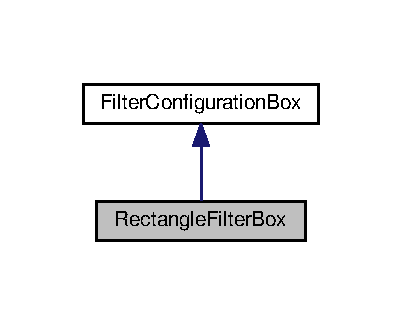
\includegraphics[width=193pt]{classGUI_1_1RectangleFilterBox__inherit__graph}
\end{center}
\end{figure}
\subsection*{Public Member Functions}
\begin{DoxyCompactItemize}
\item 
\hyperlink{classGUI_1_1RectangleFilterBox_ad1d16a75d7930e9f33f867cbed3e5815}{Rectangle\+Filter\+Box} (\hyperlink{classGUI_1_1QWidget}{G\+U\+I\+::\+Q\+Widget} $\ast$parent)
\end{DoxyCompactItemize}
\subsection*{Additional Inherited Members}


\subsection{Detailed Description}
This class contains the gui elements for changing the options of a rectangle filter. 

\subsection{Constructor \& Destructor Documentation}
\hypertarget{classGUI_1_1RectangleFilterBox_ad1d16a75d7930e9f33f867cbed3e5815}{}\index{G\+U\+I\+::\+Rectangle\+Filter\+Box@{G\+U\+I\+::\+Rectangle\+Filter\+Box}!Rectangle\+Filter\+Box@{Rectangle\+Filter\+Box}}
\index{Rectangle\+Filter\+Box@{Rectangle\+Filter\+Box}!G\+U\+I\+::\+Rectangle\+Filter\+Box@{G\+U\+I\+::\+Rectangle\+Filter\+Box}}
\subsubsection[{Rectangle\+Filter\+Box}]{\setlength{\rightskip}{0pt plus 5cm}{\bf Rectangle\+Filter\+Box} (
\begin{DoxyParamCaption}
\item[{{\bf G\+U\+I\+::\+Q\+Widget} $\ast$}]{parent}
\end{DoxyParamCaption}
)}\label{classGUI_1_1RectangleFilterBox_ad1d16a75d7930e9f33f867cbed3e5815}


Constructor. 


\hypertarget{classUndo__Redo_1_1RemoveFilter}{}\section{Remove\+Filter Class Reference}
\label{classUndo__Redo_1_1RemoveFilter}\index{Remove\+Filter@{Remove\+Filter}}
\subsection*{Public Member Functions}
\begin{DoxyCompactItemize}
\item 
\hyperlink{classUndo__Redo_1_1RemoveFilter_a910ad5d71db3e7f92d5c94072f050b3e}{Remove\+Filter} ()
\item 
void \hyperlink{classUndo__Redo_1_1RemoveFilter_a0e1e7804a53f6d62efc72c9bdbec8571}{undo} ()
\item 
void \hyperlink{classUndo__Redo_1_1RemoveFilter_a93c48d6ed036e1a381be53ac67643284}{redo} ()
\end{DoxyCompactItemize}


\subsection{Constructor \& Destructor Documentation}
\hypertarget{classUndo__Redo_1_1RemoveFilter_a910ad5d71db3e7f92d5c94072f050b3e}{}\index{Undo\+\_\+\+Redo\+::\+Remove\+Filter@{Undo\+\_\+\+Redo\+::\+Remove\+Filter}!Remove\+Filter@{Remove\+Filter}}
\index{Remove\+Filter@{Remove\+Filter}!Undo\+\_\+\+Redo\+::\+Remove\+Filter@{Undo\+\_\+\+Redo\+::\+Remove\+Filter}}
\subsubsection[{Remove\+Filter}]{\setlength{\rightskip}{0pt plus 5cm}{\bf Remove\+Filter} (
\begin{DoxyParamCaption}
{}
\end{DoxyParamCaption}
)}\label{classUndo__Redo_1_1RemoveFilter_a910ad5d71db3e7f92d5c94072f050b3e}


Constuctor 



\subsection{Member Function Documentation}
\hypertarget{classUndo__Redo_1_1RemoveFilter_a93c48d6ed036e1a381be53ac67643284}{}\index{Undo\+\_\+\+Redo\+::\+Remove\+Filter@{Undo\+\_\+\+Redo\+::\+Remove\+Filter}!redo@{redo}}
\index{redo@{redo}!Undo\+\_\+\+Redo\+::\+Remove\+Filter@{Undo\+\_\+\+Redo\+::\+Remove\+Filter}}
\subsubsection[{redo}]{\setlength{\rightskip}{0pt plus 5cm}void redo (
\begin{DoxyParamCaption}
{}
\end{DoxyParamCaption}
)}\label{classUndo__Redo_1_1RemoveFilter_a93c48d6ed036e1a381be53ac67643284}


removes a filter from the filterlist 

\hypertarget{classUndo__Redo_1_1RemoveFilter_a0e1e7804a53f6d62efc72c9bdbec8571}{}\index{Undo\+\_\+\+Redo\+::\+Remove\+Filter@{Undo\+\_\+\+Redo\+::\+Remove\+Filter}!undo@{undo}}
\index{undo@{undo}!Undo\+\_\+\+Redo\+::\+Remove\+Filter@{Undo\+\_\+\+Redo\+::\+Remove\+Filter}}
\subsubsection[{undo}]{\setlength{\rightskip}{0pt plus 5cm}void undo (
\begin{DoxyParamCaption}
{}
\end{DoxyParamCaption}
)}\label{classUndo__Redo_1_1RemoveFilter_a0e1e7804a53f6d62efc72c9bdbec8571}


adds the removed filter back into the filterlist 


\hypertarget{classUndo__Redo_1_1RemoveVideo}{}\section{Remove\+Video Class Reference}
\label{classUndo__Redo_1_1RemoveVideo}\index{Remove\+Video@{Remove\+Video}}
\subsection*{Public Member Functions}
\begin{DoxyCompactItemize}
\item 
\hyperlink{classUndo__Redo_1_1RemoveVideo_a2e45e4eb2fb6b3fae5e221b9fa71007c}{Remove\+Video} ()
\item 
void \hyperlink{classUndo__Redo_1_1RemoveVideo_a0e1e7804a53f6d62efc72c9bdbec8571}{undo} ()
\item 
void \hyperlink{classUndo__Redo_1_1RemoveVideo_a93c48d6ed036e1a381be53ac67643284}{redo} ()
\end{DoxyCompactItemize}


\subsection{Constructor \& Destructor Documentation}
\hypertarget{classUndo__Redo_1_1RemoveVideo_a2e45e4eb2fb6b3fae5e221b9fa71007c}{}\index{Undo\+\_\+\+Redo\+::\+Remove\+Video@{Undo\+\_\+\+Redo\+::\+Remove\+Video}!Remove\+Video@{Remove\+Video}}
\index{Remove\+Video@{Remove\+Video}!Undo\+\_\+\+Redo\+::\+Remove\+Video@{Undo\+\_\+\+Redo\+::\+Remove\+Video}}
\subsubsection[{Remove\+Video}]{\setlength{\rightskip}{0pt plus 5cm}{\bf Remove\+Video} (
\begin{DoxyParamCaption}
{}
\end{DoxyParamCaption}
)}\label{classUndo__Redo_1_1RemoveVideo_a2e45e4eb2fb6b3fae5e221b9fa71007c}


Constuctor 



\subsection{Member Function Documentation}
\hypertarget{classUndo__Redo_1_1RemoveVideo_a93c48d6ed036e1a381be53ac67643284}{}\index{Undo\+\_\+\+Redo\+::\+Remove\+Video@{Undo\+\_\+\+Redo\+::\+Remove\+Video}!redo@{redo}}
\index{redo@{redo}!Undo\+\_\+\+Redo\+::\+Remove\+Video@{Undo\+\_\+\+Redo\+::\+Remove\+Video}}
\subsubsection[{redo}]{\setlength{\rightskip}{0pt plus 5cm}void redo (
\begin{DoxyParamCaption}
{}
\end{DoxyParamCaption}
)}\label{classUndo__Redo_1_1RemoveVideo_a93c48d6ed036e1a381be53ac67643284}


removes a video from the analysis tab 

\hypertarget{classUndo__Redo_1_1RemoveVideo_a0e1e7804a53f6d62efc72c9bdbec8571}{}\index{Undo\+\_\+\+Redo\+::\+Remove\+Video@{Undo\+\_\+\+Redo\+::\+Remove\+Video}!undo@{undo}}
\index{undo@{undo}!Undo\+\_\+\+Redo\+::\+Remove\+Video@{Undo\+\_\+\+Redo\+::\+Remove\+Video}}
\subsubsection[{undo}]{\setlength{\rightskip}{0pt plus 5cm}void undo (
\begin{DoxyParamCaption}
{}
\end{DoxyParamCaption}
)}\label{classUndo__Redo_1_1RemoveVideo_a0e1e7804a53f6d62efc72c9bdbec8571}


readds the removed video to the analysis tab 


\hypertarget{classUtility_1_1RGBDifferenceCalculator}{}\section{R\+G\+B\+Difference\+Calculator Class Reference}
\label{classUtility_1_1RGBDifferenceCalculator}\index{R\+G\+B\+Difference\+Calculator@{R\+G\+B\+Difference\+Calculator}}
\subsection*{Public Member Functions}
\begin{DoxyCompactItemize}
\item 
\hyperlink{classUtility_1_1RGBDifferenceCalculator_a769aad3f6a88d97f35f9eebfe763ee62}{R\+G\+B\+Difference\+Calculator} (\hyperlink{classGUI_1_1Player_1_1Video}{G\+U\+I\+::\+Player\+::\+Video} \&reference\+Video, \hyperlink{classGUI_1_1Player_1_1Video}{G\+U\+I\+::\+Player\+::\+Video} \&video)
\item 
void \hyperlink{classUtility_1_1RGBDifferenceCalculator_aaef52f95d194e2562f5909346428ba04}{calculate\+Video} (\hyperlink{classGUI_1_1Player_1_1Video}{G\+U\+I\+::\+Player\+::\+Video} \&target)
\end{DoxyCompactItemize}


\subsection{Detailed Description}
This class calculates the R\+G\+B-\/difference video of a video. 

\subsection{Constructor \& Destructor Documentation}
\hypertarget{classUtility_1_1RGBDifferenceCalculator_a769aad3f6a88d97f35f9eebfe763ee62}{}\index{Utility\+::\+R\+G\+B\+Difference\+Calculator@{Utility\+::\+R\+G\+B\+Difference\+Calculator}!R\+G\+B\+Difference\+Calculator@{R\+G\+B\+Difference\+Calculator}}
\index{R\+G\+B\+Difference\+Calculator@{R\+G\+B\+Difference\+Calculator}!Utility\+::\+R\+G\+B\+Difference\+Calculator@{Utility\+::\+R\+G\+B\+Difference\+Calculator}}
\subsubsection[{R\+G\+B\+Difference\+Calculator}]{\setlength{\rightskip}{0pt plus 5cm}{\bf R\+G\+B\+Difference\+Calculator} (
\begin{DoxyParamCaption}
\item[{{\bf G\+U\+I\+::\+Player\+::\+Video} \&}]{reference\+Video, }
\item[{{\bf G\+U\+I\+::\+Player\+::\+Video} \&}]{video}
\end{DoxyParamCaption}
)}\label{classUtility_1_1RGBDifferenceCalculator_a769aad3f6a88d97f35f9eebfe763ee62}


Constructor. 


\begin{DoxyParams}{Parameters}
{\em reference\+Video} & The reference video.\\
\hline
{\em video} & The video that is compared to the reference video.\\
\hline
\end{DoxyParams}


\subsection{Member Function Documentation}
\hypertarget{classUtility_1_1RGBDifferenceCalculator_aaef52f95d194e2562f5909346428ba04}{}\index{Utility\+::\+R\+G\+B\+Difference\+Calculator@{Utility\+::\+R\+G\+B\+Difference\+Calculator}!calculate\+Video@{calculate\+Video}}
\index{calculate\+Video@{calculate\+Video}!Utility\+::\+R\+G\+B\+Difference\+Calculator@{Utility\+::\+R\+G\+B\+Difference\+Calculator}}
\subsubsection[{calculate\+Video}]{\setlength{\rightskip}{0pt plus 5cm}void calculate\+Video (
\begin{DoxyParamCaption}
\item[{{\bf G\+U\+I\+::\+Player\+::\+Video} \&}]{target}
\end{DoxyParamCaption}
)}\label{classUtility_1_1RGBDifferenceCalculator_aaef52f95d194e2562f5909346428ba04}


Calculates the R\+G\+B difference between two videos. 


\begin{DoxyParams}{Parameters}
{\em target} & the video the calculated frames are added to\\
\hline
\end{DoxyParams}

\hypertarget{classModel_1_1Filter_1_1RGBFilter}{}\section{R\+G\+B\+Filter Class Reference}
\label{classModel_1_1Filter_1_1RGBFilter}\index{R\+G\+B\+Filter@{R\+G\+B\+Filter}}
\subsection*{Public Member Functions}
\begin{DoxyCompactItemize}
\item 
\hyperlink{classModel_1_1Filter_1_1RGBFilter_a9065d7c86503c630a3422f5db4af723f}{R\+G\+B\+Filter} ()
\item 
string \hyperlink{classModel_1_1Filter_1_1RGBFilter_a62b7b60e24f92234393b840b35808e06}{get\+Filter\+Description} ()
\item 
\hyperlink{namespaceModel_1_1Filter_a54742b2fc8f6a246926cbb87b7fae1a4}{Model\+::\+Filter\+::\+Basic\+Color} \hyperlink{classModel_1_1Filter_1_1RGBFilter_a82047004348409d221728e88c0b9dfa7}{get\+Color} ()
\item 
void \hyperlink{classModel_1_1Filter_1_1RGBFilter_a353ae5c263a046f9ef3b72438cfecd95}{set\+Color} (\hyperlink{namespaceModel_1_1Filter_a54742b2fc8f6a246926cbb87b7fae1a4}{Model\+::\+Filter\+::\+Basic\+Color} color)
\item 
string \hyperlink{classModel_1_1Filter_1_1RGBFilter_a11335e13e50af74108bf926dc1340b4b}{get\+Name} ()
\end{DoxyCompactItemize}
\subsection*{Additional Inherited Members}


\subsection{Detailed Description}
Filters the video by a given channel (red, green or blue). 

\subsection{Constructor \& Destructor Documentation}
\hypertarget{classModel_1_1Filter_1_1RGBFilter_a9065d7c86503c630a3422f5db4af723f}{}\index{Model\+::\+Filter\+::\+R\+G\+B\+Filter@{Model\+::\+Filter\+::\+R\+G\+B\+Filter}!R\+G\+B\+Filter@{R\+G\+B\+Filter}}
\index{R\+G\+B\+Filter@{R\+G\+B\+Filter}!Model\+::\+Filter\+::\+R\+G\+B\+Filter@{Model\+::\+Filter\+::\+R\+G\+B\+Filter}}
\subsubsection[{R\+G\+B\+Filter}]{\setlength{\rightskip}{0pt plus 5cm}{\bf R\+G\+B\+Filter} (
\begin{DoxyParamCaption}
{}
\end{DoxyParamCaption}
)}\label{classModel_1_1Filter_1_1RGBFilter_a9065d7c86503c630a3422f5db4af723f}


Constructor. 



\subsection{Member Function Documentation}
\hypertarget{classModel_1_1Filter_1_1RGBFilter_a82047004348409d221728e88c0b9dfa7}{}\index{Model\+::\+Filter\+::\+R\+G\+B\+Filter@{Model\+::\+Filter\+::\+R\+G\+B\+Filter}!get\+Color@{get\+Color}}
\index{get\+Color@{get\+Color}!Model\+::\+Filter\+::\+R\+G\+B\+Filter@{Model\+::\+Filter\+::\+R\+G\+B\+Filter}}
\subsubsection[{get\+Color}]{\setlength{\rightskip}{0pt plus 5cm}{\bf Model\+::\+Filter\+::\+Basic\+Color} get\+Color (
\begin{DoxyParamCaption}
{}
\end{DoxyParamCaption}
)}\label{classModel_1_1Filter_1_1RGBFilter_a82047004348409d221728e88c0b9dfa7}


Returns the color that is not filtered out. 

\begin{DoxyReturn}{Returns}
The preserved color.
\end{DoxyReturn}
\hypertarget{classModel_1_1Filter_1_1RGBFilter_a62b7b60e24f92234393b840b35808e06}{}\index{Model\+::\+Filter\+::\+R\+G\+B\+Filter@{Model\+::\+Filter\+::\+R\+G\+B\+Filter}!get\+Filter\+Description@{get\+Filter\+Description}}
\index{get\+Filter\+Description@{get\+Filter\+Description}!Model\+::\+Filter\+::\+R\+G\+B\+Filter@{Model\+::\+Filter\+::\+R\+G\+B\+Filter}}
\subsubsection[{get\+Filter\+Description}]{\setlength{\rightskip}{0pt plus 5cm}string get\+Filter\+Description (
\begin{DoxyParamCaption}
{}
\end{DoxyParamCaption}
)\hspace{0.3cm}{\ttfamily [virtual]}}\label{classModel_1_1Filter_1_1RGBFilter_a62b7b60e24f92234393b840b35808e06}


Returns the string that the ffmpeg library needs to apply the filter to a video. 

\begin{DoxyReturn}{Returns}
The string for the ffmpeg library.
\end{DoxyReturn}


Implements \hyperlink{classModel_1_1Filter_1_1Filter_a453fcafa809afa1ce58d9ef95d5f26c0}{Filter}.

\hypertarget{classModel_1_1Filter_1_1RGBFilter_a11335e13e50af74108bf926dc1340b4b}{}\index{Model\+::\+Filter\+::\+R\+G\+B\+Filter@{Model\+::\+Filter\+::\+R\+G\+B\+Filter}!get\+Name@{get\+Name}}
\index{get\+Name@{get\+Name}!Model\+::\+Filter\+::\+R\+G\+B\+Filter@{Model\+::\+Filter\+::\+R\+G\+B\+Filter}}
\subsubsection[{get\+Name}]{\setlength{\rightskip}{0pt plus 5cm}string get\+Name (
\begin{DoxyParamCaption}
{}
\end{DoxyParamCaption}
)\hspace{0.3cm}{\ttfamily [virtual]}}\label{classModel_1_1Filter_1_1RGBFilter_a11335e13e50af74108bf926dc1340b4b}


Returns the name of the filter. 

\begin{DoxyReturn}{Returns}
The filtername.
\end{DoxyReturn}


Implements \hyperlink{classModel_1_1Filter_1_1Filter_ade93aa98c68d185a9c03784d36140225}{Filter}.

\hypertarget{classModel_1_1Filter_1_1RGBFilter_a353ae5c263a046f9ef3b72438cfecd95}{}\index{Model\+::\+Filter\+::\+R\+G\+B\+Filter@{Model\+::\+Filter\+::\+R\+G\+B\+Filter}!set\+Color@{set\+Color}}
\index{set\+Color@{set\+Color}!Model\+::\+Filter\+::\+R\+G\+B\+Filter@{Model\+::\+Filter\+::\+R\+G\+B\+Filter}}
\subsubsection[{set\+Color}]{\setlength{\rightskip}{0pt plus 5cm}void set\+Color (
\begin{DoxyParamCaption}
\item[{{\bf Model\+::\+Filter\+::\+Basic\+Color}}]{color}
\end{DoxyParamCaption}
)}\label{classModel_1_1Filter_1_1RGBFilter_a353ae5c263a046f9ef3b72438cfecd95}


Sets the preserved color. 


\begin{DoxyParams}{Parameters}
{\em color} & The preserved color.\\
\hline
\end{DoxyParams}

\hypertarget{classGUI_1_1RGBFilterBox}{}\section{R\+G\+B\+Filter\+Box Class Reference}
\label{classGUI_1_1RGBFilterBox}\index{R\+G\+B\+Filter\+Box@{R\+G\+B\+Filter\+Box}}
\subsection*{Public Member Functions}
\begin{DoxyCompactItemize}
\item 
\hyperlink{classGUI_1_1RGBFilterBox_a2bd622e6f8727ea01b985e13e407d6ac}{R\+G\+B\+Filter\+Box} (\hyperlink{classGUI_1_1Player_1_1QWidget}{G\+U\+I\+::\+Player\+::\+Q\+Widget} $\ast$parent)
\end{DoxyCompactItemize}
\subsection*{Additional Inherited Members}


\subsection{Detailed Description}
This class contains the gui elements for changing the options of a rgb filter. 

\subsection{Constructor \& Destructor Documentation}
\hypertarget{classGUI_1_1RGBFilterBox_a2bd622e6f8727ea01b985e13e407d6ac}{}\index{G\+U\+I\+::\+R\+G\+B\+Filter\+Box@{G\+U\+I\+::\+R\+G\+B\+Filter\+Box}!R\+G\+B\+Filter\+Box@{R\+G\+B\+Filter\+Box}}
\index{R\+G\+B\+Filter\+Box@{R\+G\+B\+Filter\+Box}!G\+U\+I\+::\+R\+G\+B\+Filter\+Box@{G\+U\+I\+::\+R\+G\+B\+Filter\+Box}}
\subsubsection[{R\+G\+B\+Filter\+Box}]{\setlength{\rightskip}{0pt plus 5cm}{\bf R\+G\+B\+Filter\+Box} (
\begin{DoxyParamCaption}
\item[{{\bf G\+U\+I\+::\+Player\+::\+Q\+Widget} $\ast$}]{parent}
\end{DoxyParamCaption}
)}\label{classGUI_1_1RGBFilterBox_a2bd622e6f8727ea01b985e13e407d6ac}


Constructor. 


\hypertarget{classUtility_1_1RGBHistogrammCalculator}{}\section{R\+G\+B\+Histogramm\+Calculator Class Reference}
\label{classUtility_1_1RGBHistogrammCalculator}\index{R\+G\+B\+Histogramm\+Calculator@{R\+G\+B\+Histogramm\+Calculator}}
\subsection*{Public Member Functions}
\begin{DoxyCompactItemize}
\item 
void \hyperlink{classUtility_1_1RGBHistogrammCalculator_a0c01f44967ccf0d367f88a1bfd72c701}{R\+G\+B\+Historgramm\+Calculator} (\hyperlink{classGUI_1_1Player_1_1Video}{G\+U\+I\+::\+Player\+::\+Video} \&video)
\item 
void \hyperlink{classUtility_1_1RGBHistogrammCalculator_afe1d8348c24e6589bc7c0b3f689316a7}{calculate} ()
\item 
\hyperlink{classModel_1_1Graph}{Model\+::\+Graph} \hyperlink{classUtility_1_1RGBHistogrammCalculator_a11345d1b2b32275950a10525c1e0e9d1}{get\+Red\+Histogramm} ()
\item 
\hyperlink{classModel_1_1Graph}{Model\+::\+Graph} \hyperlink{classUtility_1_1RGBHistogrammCalculator_a84bbb0085709b08aef6f9f2a849dcf10}{get\+Green\+Histogramm} ()
\item 
\hyperlink{classModel_1_1Graph}{Model\+::\+Graph} \hyperlink{classUtility_1_1RGBHistogrammCalculator_a6bc6a7ac3d5da8080b9c5f146c0d4e8f}{get\+Blue\+Histogramm} ()
\end{DoxyCompactItemize}


\subsection{Detailed Description}
This class calculates the R\+G\+B histogramm for a video. 

\subsection{Member Function Documentation}
\hypertarget{classUtility_1_1RGBHistogrammCalculator_afe1d8348c24e6589bc7c0b3f689316a7}{}\index{Utility\+::\+R\+G\+B\+Histogramm\+Calculator@{Utility\+::\+R\+G\+B\+Histogramm\+Calculator}!calculate@{calculate}}
\index{calculate@{calculate}!Utility\+::\+R\+G\+B\+Histogramm\+Calculator@{Utility\+::\+R\+G\+B\+Histogramm\+Calculator}}
\subsubsection[{calculate}]{\setlength{\rightskip}{0pt plus 5cm}void calculate (
\begin{DoxyParamCaption}
{}
\end{DoxyParamCaption}
)}\label{classUtility_1_1RGBHistogrammCalculator_afe1d8348c24e6589bc7c0b3f689316a7}


Calculates the red, green and blue components of a video. 

\hypertarget{classUtility_1_1RGBHistogrammCalculator_a6bc6a7ac3d5da8080b9c5f146c0d4e8f}{}\index{Utility\+::\+R\+G\+B\+Histogramm\+Calculator@{Utility\+::\+R\+G\+B\+Histogramm\+Calculator}!get\+Blue\+Histogramm@{get\+Blue\+Histogramm}}
\index{get\+Blue\+Histogramm@{get\+Blue\+Histogramm}!Utility\+::\+R\+G\+B\+Histogramm\+Calculator@{Utility\+::\+R\+G\+B\+Histogramm\+Calculator}}
\subsubsection[{get\+Blue\+Histogramm}]{\setlength{\rightskip}{0pt plus 5cm}{\bf Model\+::\+Graph} get\+Blue\+Histogramm (
\begin{DoxyParamCaption}
{}
\end{DoxyParamCaption}
)}\label{classUtility_1_1RGBHistogrammCalculator_a6bc6a7ac3d5da8080b9c5f146c0d4e8f}


Returns the blue components of a video. 

\hypertarget{classUtility_1_1RGBHistogrammCalculator_a84bbb0085709b08aef6f9f2a849dcf10}{}\index{Utility\+::\+R\+G\+B\+Histogramm\+Calculator@{Utility\+::\+R\+G\+B\+Histogramm\+Calculator}!get\+Green\+Histogramm@{get\+Green\+Histogramm}}
\index{get\+Green\+Histogramm@{get\+Green\+Histogramm}!Utility\+::\+R\+G\+B\+Histogramm\+Calculator@{Utility\+::\+R\+G\+B\+Histogramm\+Calculator}}
\subsubsection[{get\+Green\+Histogramm}]{\setlength{\rightskip}{0pt plus 5cm}{\bf Model\+::\+Graph} get\+Green\+Histogramm (
\begin{DoxyParamCaption}
{}
\end{DoxyParamCaption}
)}\label{classUtility_1_1RGBHistogrammCalculator_a84bbb0085709b08aef6f9f2a849dcf10}


Returns the green components of a video. 

\hypertarget{classUtility_1_1RGBHistogrammCalculator_a11345d1b2b32275950a10525c1e0e9d1}{}\index{Utility\+::\+R\+G\+B\+Histogramm\+Calculator@{Utility\+::\+R\+G\+B\+Histogramm\+Calculator}!get\+Red\+Histogramm@{get\+Red\+Histogramm}}
\index{get\+Red\+Histogramm@{get\+Red\+Histogramm}!Utility\+::\+R\+G\+B\+Histogramm\+Calculator@{Utility\+::\+R\+G\+B\+Histogramm\+Calculator}}
\subsubsection[{get\+Red\+Histogramm}]{\setlength{\rightskip}{0pt plus 5cm}{\bf Model\+::\+Graph} get\+Red\+Histogramm (
\begin{DoxyParamCaption}
{}
\end{DoxyParamCaption}
)}\label{classUtility_1_1RGBHistogrammCalculator_a11345d1b2b32275950a10525c1e0e9d1}


Returns the red components of a video. 

\hypertarget{classUtility_1_1RGBHistogrammCalculator_a0c01f44967ccf0d367f88a1bfd72c701}{}\index{Utility\+::\+R\+G\+B\+Histogramm\+Calculator@{Utility\+::\+R\+G\+B\+Histogramm\+Calculator}!R\+G\+B\+Historgramm\+Calculator@{R\+G\+B\+Historgramm\+Calculator}}
\index{R\+G\+B\+Historgramm\+Calculator@{R\+G\+B\+Historgramm\+Calculator}!Utility\+::\+R\+G\+B\+Histogramm\+Calculator@{Utility\+::\+R\+G\+B\+Histogramm\+Calculator}}
\subsubsection[{R\+G\+B\+Historgramm\+Calculator}]{\setlength{\rightskip}{0pt plus 5cm}void R\+G\+B\+Historgramm\+Calculator (
\begin{DoxyParamCaption}
\item[{{\bf G\+U\+I\+::\+Player\+::\+Video} \&}]{video}
\end{DoxyParamCaption}
)}\label{classUtility_1_1RGBHistogrammCalculator_a0c01f44967ccf0d367f88a1bfd72c701}


Constructor. 


\begin{DoxyParams}{Parameters}
{\em video} & the video that is analyzed.\\
\hline
\end{DoxyParams}

\hypertarget{classModel_1_1Filter_1_1RotationFilter}{}\section{Rotation\+Filter Class Reference}
\label{classModel_1_1Filter_1_1RotationFilter}\index{Rotation\+Filter@{Rotation\+Filter}}
\subsection*{Public Member Functions}
\begin{DoxyCompactItemize}
\item 
std\+::string \hyperlink{classModel_1_1Filter_1_1RotationFilter_a2b3f7d8fcd3d774b4a2fde5914a9729f}{get\+Filter\+Description} ()
\item 
\hypertarget{classModel_1_1Filter_1_1RotationFilter_ae71094a2b50726fbec9d9475b2c92e01}{}int {\bfseries get\+Angle} ()\label{classModel_1_1Filter_1_1RotationFilter_ae71094a2b50726fbec9d9475b2c92e01}

\item 
std\+::string \hyperlink{classModel_1_1Filter_1_1RotationFilter_ac0fc966d4386ddb71d99361e3fccb311}{get\+Name} ()
\item 
\hypertarget{classModel_1_1Filter_1_1RotationFilter_a241a28cb2a44be5be3440363436be22f}{}void {\bfseries set\+Angle} (int angle)\label{classModel_1_1Filter_1_1RotationFilter_a241a28cb2a44be5be3440363436be22f}

\end{DoxyCompactItemize}


\subsection{Detailed Description}
Rotates the video 

\subsection{Member Function Documentation}
\hypertarget{classModel_1_1Filter_1_1RotationFilter_a2b3f7d8fcd3d774b4a2fde5914a9729f}{}\index{Model\+::\+Filter\+::\+Rotation\+Filter@{Model\+::\+Filter\+::\+Rotation\+Filter}!get\+Filter\+Description@{get\+Filter\+Description}}
\index{get\+Filter\+Description@{get\+Filter\+Description}!Model\+::\+Filter\+::\+Rotation\+Filter@{Model\+::\+Filter\+::\+Rotation\+Filter}}
\subsubsection[{get\+Filter\+Description}]{\setlength{\rightskip}{0pt plus 5cm}std\+::string get\+Filter\+Description (
\begin{DoxyParamCaption}
{}
\end{DoxyParamCaption}
)\hspace{0.3cm}{\ttfamily [virtual]}}\label{classModel_1_1Filter_1_1RotationFilter_a2b3f7d8fcd3d774b4a2fde5914a9729f}


Returns the description of the filter 



Implements \hyperlink{classModel_1_1Filter_1_1Filter_ad400dc313dea3f9d3838d078ea4d2590}{Filter}.

\hypertarget{classModel_1_1Filter_1_1RotationFilter_ac0fc966d4386ddb71d99361e3fccb311}{}\index{Model\+::\+Filter\+::\+Rotation\+Filter@{Model\+::\+Filter\+::\+Rotation\+Filter}!get\+Name@{get\+Name}}
\index{get\+Name@{get\+Name}!Model\+::\+Filter\+::\+Rotation\+Filter@{Model\+::\+Filter\+::\+Rotation\+Filter}}
\subsubsection[{get\+Name}]{\setlength{\rightskip}{0pt plus 5cm}std\+::string get\+Name (
\begin{DoxyParamCaption}
{}
\end{DoxyParamCaption}
)\hspace{0.3cm}{\ttfamily [virtual]}}\label{classModel_1_1Filter_1_1RotationFilter_ac0fc966d4386ddb71d99361e3fccb311}


Returns the name of the filter 



Implements \hyperlink{classModel_1_1Filter_1_1Filter_ab7a5c5c512dadd4cbd18dd1b0f42e930}{Filter}.


\hypertarget{classGUI_1_1RotationFilterBox}{}\section{Rotation\+Filter\+Box Class Reference}
\label{classGUI_1_1RotationFilterBox}\index{Rotation\+Filter\+Box@{Rotation\+Filter\+Box}}


Inheritance diagram for Rotation\+Filter\+Box\+:
\nopagebreak
\begin{figure}[H]
\begin{center}
\leavevmode
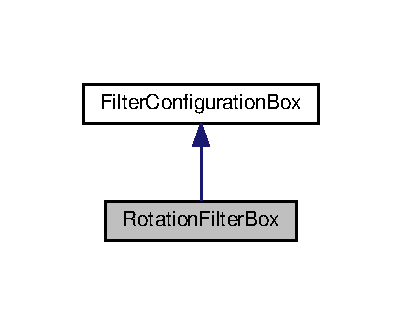
\includegraphics[width=193pt]{classGUI_1_1RotationFilterBox__inherit__graph}
\end{center}
\end{figure}
\subsection*{Public Member Functions}
\begin{DoxyCompactItemize}
\item 
\hyperlink{classGUI_1_1RotationFilterBox_a86a39151a9e0eae3f619853f8469db4e}{Rotation\+Filter\+Box} (\hyperlink{classGUI_1_1QWidget}{G\+U\+I\+::\+Q\+Widget} $\ast$parent)
\end{DoxyCompactItemize}
\subsection*{Additional Inherited Members}


\subsection{Detailed Description}
This class contains the gui elements for changing the options of a rotation filter. 

\subsection{Constructor \& Destructor Documentation}
\hypertarget{classGUI_1_1RotationFilterBox_a86a39151a9e0eae3f619853f8469db4e}{}\index{G\+U\+I\+::\+Rotation\+Filter\+Box@{G\+U\+I\+::\+Rotation\+Filter\+Box}!Rotation\+Filter\+Box@{Rotation\+Filter\+Box}}
\index{Rotation\+Filter\+Box@{Rotation\+Filter\+Box}!G\+U\+I\+::\+Rotation\+Filter\+Box@{G\+U\+I\+::\+Rotation\+Filter\+Box}}
\subsubsection[{Rotation\+Filter\+Box}]{\setlength{\rightskip}{0pt plus 5cm}{\bf Rotation\+Filter\+Box} (
\begin{DoxyParamCaption}
\item[{{\bf G\+U\+I\+::\+Q\+Widget} $\ast$}]{parent}
\end{DoxyParamCaption}
)}\label{classGUI_1_1RotationFilterBox_a86a39151a9e0eae3f619853f8469db4e}


Constructor. 


\hypertarget{classModel_1_1Filter_1_1SaturationFilter}{}\section{Saturation\+Filter Class Reference}
\label{classModel_1_1Filter_1_1SaturationFilter}\index{Saturation\+Filter@{Saturation\+Filter}}
\subsection*{Public Member Functions}
\begin{DoxyCompactItemize}
\item 
\hyperlink{classModel_1_1Filter_1_1SaturationFilter_ae45fd836bb8ade0550727f4060bdffa9}{Saturation\+Filter} ()
\item 
string \hyperlink{classModel_1_1Filter_1_1SaturationFilter_a62b7b60e24f92234393b840b35808e06}{get\+Filter\+Description} ()
\item 
int \hyperlink{classModel_1_1Filter_1_1SaturationFilter_a708995fb1b6acb31ee0dfb0f4881e5b5}{get\+Intensity} ()
\item 
string \hyperlink{classModel_1_1Filter_1_1SaturationFilter_a11335e13e50af74108bf926dc1340b4b}{get\+Name} ()
\item 
void \hyperlink{classModel_1_1Filter_1_1SaturationFilter_ac8255ffbc46bb61acaa8fd23d0d260eb}{set\+Intensity} (int intensity)
\end{DoxyCompactItemize}
\subsection*{Additional Inherited Members}


\subsection{Detailed Description}
Adjusts the saturation of the video. 

\subsection{Constructor \& Destructor Documentation}
\hypertarget{classModel_1_1Filter_1_1SaturationFilter_ae45fd836bb8ade0550727f4060bdffa9}{}\index{Model\+::\+Filter\+::\+Saturation\+Filter@{Model\+::\+Filter\+::\+Saturation\+Filter}!Saturation\+Filter@{Saturation\+Filter}}
\index{Saturation\+Filter@{Saturation\+Filter}!Model\+::\+Filter\+::\+Saturation\+Filter@{Model\+::\+Filter\+::\+Saturation\+Filter}}
\subsubsection[{Saturation\+Filter}]{\setlength{\rightskip}{0pt plus 5cm}{\bf Saturation\+Filter} (
\begin{DoxyParamCaption}
{}
\end{DoxyParamCaption}
)}\label{classModel_1_1Filter_1_1SaturationFilter_ae45fd836bb8ade0550727f4060bdffa9}


Constructor. 



\subsection{Member Function Documentation}
\hypertarget{classModel_1_1Filter_1_1SaturationFilter_a62b7b60e24f92234393b840b35808e06}{}\index{Model\+::\+Filter\+::\+Saturation\+Filter@{Model\+::\+Filter\+::\+Saturation\+Filter}!get\+Filter\+Description@{get\+Filter\+Description}}
\index{get\+Filter\+Description@{get\+Filter\+Description}!Model\+::\+Filter\+::\+Saturation\+Filter@{Model\+::\+Filter\+::\+Saturation\+Filter}}
\subsubsection[{get\+Filter\+Description}]{\setlength{\rightskip}{0pt plus 5cm}string get\+Filter\+Description (
\begin{DoxyParamCaption}
{}
\end{DoxyParamCaption}
)\hspace{0.3cm}{\ttfamily [virtual]}}\label{classModel_1_1Filter_1_1SaturationFilter_a62b7b60e24f92234393b840b35808e06}


Returns the string that the ffmpeg library needs to apply the filter to a video. 

\begin{DoxyReturn}{Returns}
The string for the ffmpeg library.
\end{DoxyReturn}


Implements \hyperlink{classModel_1_1Filter_1_1Filter_a453fcafa809afa1ce58d9ef95d5f26c0}{Filter}.

\hypertarget{classModel_1_1Filter_1_1SaturationFilter_a708995fb1b6acb31ee0dfb0f4881e5b5}{}\index{Model\+::\+Filter\+::\+Saturation\+Filter@{Model\+::\+Filter\+::\+Saturation\+Filter}!get\+Intensity@{get\+Intensity}}
\index{get\+Intensity@{get\+Intensity}!Model\+::\+Filter\+::\+Saturation\+Filter@{Model\+::\+Filter\+::\+Saturation\+Filter}}
\subsubsection[{get\+Intensity}]{\setlength{\rightskip}{0pt plus 5cm}int get\+Intensity (
\begin{DoxyParamCaption}
{}
\end{DoxyParamCaption}
)}\label{classModel_1_1Filter_1_1SaturationFilter_a708995fb1b6acb31ee0dfb0f4881e5b5}


Returns the intensity of the saturation. 

\begin{DoxyReturn}{Returns}
The intensity.
\end{DoxyReturn}
\hypertarget{classModel_1_1Filter_1_1SaturationFilter_a11335e13e50af74108bf926dc1340b4b}{}\index{Model\+::\+Filter\+::\+Saturation\+Filter@{Model\+::\+Filter\+::\+Saturation\+Filter}!get\+Name@{get\+Name}}
\index{get\+Name@{get\+Name}!Model\+::\+Filter\+::\+Saturation\+Filter@{Model\+::\+Filter\+::\+Saturation\+Filter}}
\subsubsection[{get\+Name}]{\setlength{\rightskip}{0pt plus 5cm}string get\+Name (
\begin{DoxyParamCaption}
{}
\end{DoxyParamCaption}
)\hspace{0.3cm}{\ttfamily [virtual]}}\label{classModel_1_1Filter_1_1SaturationFilter_a11335e13e50af74108bf926dc1340b4b}


Returns the name of the filter. 

\begin{DoxyReturn}{Returns}
The filtername.
\end{DoxyReturn}


Implements \hyperlink{classModel_1_1Filter_1_1Filter_ade93aa98c68d185a9c03784d36140225}{Filter}.

\hypertarget{classModel_1_1Filter_1_1SaturationFilter_ac8255ffbc46bb61acaa8fd23d0d260eb}{}\index{Model\+::\+Filter\+::\+Saturation\+Filter@{Model\+::\+Filter\+::\+Saturation\+Filter}!set\+Intensity@{set\+Intensity}}
\index{set\+Intensity@{set\+Intensity}!Model\+::\+Filter\+::\+Saturation\+Filter@{Model\+::\+Filter\+::\+Saturation\+Filter}}
\subsubsection[{set\+Intensity}]{\setlength{\rightskip}{0pt plus 5cm}void set\+Intensity (
\begin{DoxyParamCaption}
\item[{int}]{intensity}
\end{DoxyParamCaption}
)}\label{classModel_1_1Filter_1_1SaturationFilter_ac8255ffbc46bb61acaa8fd23d0d260eb}


Sets the intensity of the saturation. 


\begin{DoxyParams}{Parameters}
{\em intensity} & The new intensity,\\
\hline
\end{DoxyParams}

\hypertarget{classGUI_1_1SaturationFilterBox}{}\section{Saturation\+Filter\+Box Class Reference}
\label{classGUI_1_1SaturationFilterBox}\index{Saturation\+Filter\+Box@{Saturation\+Filter\+Box}}


Inheritance diagram for Saturation\+Filter\+Box\+:
\nopagebreak
\begin{figure}[H]
\begin{center}
\leavevmode
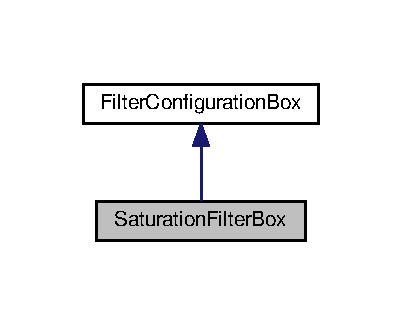
\includegraphics[width=193pt]{classGUI_1_1SaturationFilterBox__inherit__graph}
\end{center}
\end{figure}
\subsection*{Public Member Functions}
\begin{DoxyCompactItemize}
\item 
\hyperlink{classGUI_1_1SaturationFilterBox_aedb403a0d62fc7b393637eceb4e7eecb}{Saturation\+Filter\+Box} (\hyperlink{classGUI_1_1QWidget}{G\+U\+I\+::\+Q\+Widget} $\ast$parent)
\end{DoxyCompactItemize}
\subsection*{Additional Inherited Members}


\subsection{Detailed Description}
This class contains the gui elements for changing the options of a saturation filter. 

\subsection{Constructor \& Destructor Documentation}
\hypertarget{classGUI_1_1SaturationFilterBox_aedb403a0d62fc7b393637eceb4e7eecb}{}\index{G\+U\+I\+::\+Saturation\+Filter\+Box@{G\+U\+I\+::\+Saturation\+Filter\+Box}!Saturation\+Filter\+Box@{Saturation\+Filter\+Box}}
\index{Saturation\+Filter\+Box@{Saturation\+Filter\+Box}!G\+U\+I\+::\+Saturation\+Filter\+Box@{G\+U\+I\+::\+Saturation\+Filter\+Box}}
\subsubsection[{Saturation\+Filter\+Box}]{\setlength{\rightskip}{0pt plus 5cm}{\bf Saturation\+Filter\+Box} (
\begin{DoxyParamCaption}
\item[{{\bf G\+U\+I\+::\+Q\+Widget} $\ast$}]{parent}
\end{DoxyParamCaption}
)}\label{classGUI_1_1SaturationFilterBox_aedb403a0d62fc7b393637eceb4e7eecb}


Constructor. 


\hypertarget{classModel_1_1Filter_1_1ScaleFilter}{}\section{Scale\+Filter Class Reference}
\label{classModel_1_1Filter_1_1ScaleFilter}\index{Scale\+Filter@{Scale\+Filter}}
\subsection*{Public Member Functions}
\begin{DoxyCompactItemize}
\item 
\hyperlink{classModel_1_1Filter_1_1ScaleFilter_a97c359581f0dd70601196694efdace5a}{Scale\+Filter} ()
\item 
string \hyperlink{classModel_1_1Filter_1_1ScaleFilter_a62b7b60e24f92234393b840b35808e06}{get\+Filter\+Description} ()
\item 
bool \hyperlink{classModel_1_1Filter_1_1ScaleFilter_a24f2abc27a0f228db8763dbecb6ad326}{get\+Keep\+Ratio} ()
\item 
void \hyperlink{classModel_1_1Filter_1_1ScaleFilter_a8a9a32b92c6a9dc160091d8886ba13dc}{set\+Keep\+Ratio} (bool keep\+Ratio)
\item 
string \hyperlink{classModel_1_1Filter_1_1ScaleFilter_a11335e13e50af74108bf926dc1340b4b}{get\+Name} ()
\item 
int \hyperlink{classModel_1_1Filter_1_1ScaleFilter_a67a0997183f24da19b776d96c1052998}{get\+Width} ()
\item 
void \hyperlink{classModel_1_1Filter_1_1ScaleFilter_a8b4c8bccc530aa0a9b0139e04913af32}{set\+Width} (int width)
\item 
int \hyperlink{classModel_1_1Filter_1_1ScaleFilter_a07efb2a4e9a982688c8bb3c3f21d1092}{get\+Height} ()
\item 
void \hyperlink{classModel_1_1Filter_1_1ScaleFilter_a7013185ad2825ade83994b396c4fdfcd}{set\+Height} (int height)
\item 
int \hyperlink{classModel_1_1Filter_1_1ScaleFilter_ae46369a45bda66dc98d82f36c3025e79}{get\+Ratio} ()
\item 
void \hyperlink{classModel_1_1Filter_1_1ScaleFilter_a862467c05166d50d0ea15bca3ca1414d}{set\+Ratio} (int ratio)
\end{DoxyCompactItemize}
\subsection*{Additional Inherited Members}


\subsection{Detailed Description}
Scales the video. 

\subsection{Constructor \& Destructor Documentation}
\hypertarget{classModel_1_1Filter_1_1ScaleFilter_a97c359581f0dd70601196694efdace5a}{}\index{Model\+::\+Filter\+::\+Scale\+Filter@{Model\+::\+Filter\+::\+Scale\+Filter}!Scale\+Filter@{Scale\+Filter}}
\index{Scale\+Filter@{Scale\+Filter}!Model\+::\+Filter\+::\+Scale\+Filter@{Model\+::\+Filter\+::\+Scale\+Filter}}
\subsubsection[{Scale\+Filter}]{\setlength{\rightskip}{0pt plus 5cm}{\bf Scale\+Filter} (
\begin{DoxyParamCaption}
{}
\end{DoxyParamCaption}
)}\label{classModel_1_1Filter_1_1ScaleFilter_a97c359581f0dd70601196694efdace5a}


Constructor. 



\subsection{Member Function Documentation}
\hypertarget{classModel_1_1Filter_1_1ScaleFilter_a62b7b60e24f92234393b840b35808e06}{}\index{Model\+::\+Filter\+::\+Scale\+Filter@{Model\+::\+Filter\+::\+Scale\+Filter}!get\+Filter\+Description@{get\+Filter\+Description}}
\index{get\+Filter\+Description@{get\+Filter\+Description}!Model\+::\+Filter\+::\+Scale\+Filter@{Model\+::\+Filter\+::\+Scale\+Filter}}
\subsubsection[{get\+Filter\+Description}]{\setlength{\rightskip}{0pt plus 5cm}string get\+Filter\+Description (
\begin{DoxyParamCaption}
{}
\end{DoxyParamCaption}
)\hspace{0.3cm}{\ttfamily [virtual]}}\label{classModel_1_1Filter_1_1ScaleFilter_a62b7b60e24f92234393b840b35808e06}


Returns the string that the ffmpeg library needs to apply the filter to a video. 

\begin{DoxyReturn}{Returns}
The string for the ffmpeg library.
\end{DoxyReturn}


Implements \hyperlink{classModel_1_1Filter_1_1Filter_a453fcafa809afa1ce58d9ef95d5f26c0}{Filter}.

\hypertarget{classModel_1_1Filter_1_1ScaleFilter_a07efb2a4e9a982688c8bb3c3f21d1092}{}\index{Model\+::\+Filter\+::\+Scale\+Filter@{Model\+::\+Filter\+::\+Scale\+Filter}!get\+Height@{get\+Height}}
\index{get\+Height@{get\+Height}!Model\+::\+Filter\+::\+Scale\+Filter@{Model\+::\+Filter\+::\+Scale\+Filter}}
\subsubsection[{get\+Height}]{\setlength{\rightskip}{0pt plus 5cm}int get\+Height (
\begin{DoxyParamCaption}
{}
\end{DoxyParamCaption}
)}\label{classModel_1_1Filter_1_1ScaleFilter_a07efb2a4e9a982688c8bb3c3f21d1092}


Returns the new height. 

\begin{DoxyReturn}{Returns}
The new height.
\end{DoxyReturn}
\hypertarget{classModel_1_1Filter_1_1ScaleFilter_a24f2abc27a0f228db8763dbecb6ad326}{}\index{Model\+::\+Filter\+::\+Scale\+Filter@{Model\+::\+Filter\+::\+Scale\+Filter}!get\+Keep\+Ratio@{get\+Keep\+Ratio}}
\index{get\+Keep\+Ratio@{get\+Keep\+Ratio}!Model\+::\+Filter\+::\+Scale\+Filter@{Model\+::\+Filter\+::\+Scale\+Filter}}
\subsubsection[{get\+Keep\+Ratio}]{\setlength{\rightskip}{0pt plus 5cm}bool get\+Keep\+Ratio (
\begin{DoxyParamCaption}
{}
\end{DoxyParamCaption}
)}\label{classModel_1_1Filter_1_1ScaleFilter_a24f2abc27a0f228db8763dbecb6ad326}


Whether the ration is preserved. 

\begin{DoxyReturn}{Returns}
True if the ration is preserved.
\end{DoxyReturn}
\hypertarget{classModel_1_1Filter_1_1ScaleFilter_a11335e13e50af74108bf926dc1340b4b}{}\index{Model\+::\+Filter\+::\+Scale\+Filter@{Model\+::\+Filter\+::\+Scale\+Filter}!get\+Name@{get\+Name}}
\index{get\+Name@{get\+Name}!Model\+::\+Filter\+::\+Scale\+Filter@{Model\+::\+Filter\+::\+Scale\+Filter}}
\subsubsection[{get\+Name}]{\setlength{\rightskip}{0pt plus 5cm}string get\+Name (
\begin{DoxyParamCaption}
{}
\end{DoxyParamCaption}
)\hspace{0.3cm}{\ttfamily [virtual]}}\label{classModel_1_1Filter_1_1ScaleFilter_a11335e13e50af74108bf926dc1340b4b}


Returns the name of the filter. 

\begin{DoxyReturn}{Returns}
The filtername.
\end{DoxyReturn}


Implements \hyperlink{classModel_1_1Filter_1_1Filter_ade93aa98c68d185a9c03784d36140225}{Filter}.

\hypertarget{classModel_1_1Filter_1_1ScaleFilter_ae46369a45bda66dc98d82f36c3025e79}{}\index{Model\+::\+Filter\+::\+Scale\+Filter@{Model\+::\+Filter\+::\+Scale\+Filter}!get\+Ratio@{get\+Ratio}}
\index{get\+Ratio@{get\+Ratio}!Model\+::\+Filter\+::\+Scale\+Filter@{Model\+::\+Filter\+::\+Scale\+Filter}}
\subsubsection[{get\+Ratio}]{\setlength{\rightskip}{0pt plus 5cm}int get\+Ratio (
\begin{DoxyParamCaption}
{}
\end{DoxyParamCaption}
)}\label{classModel_1_1Filter_1_1ScaleFilter_ae46369a45bda66dc98d82f36c3025e79}


Returns the ratio of the scaling. 

\begin{DoxyReturn}{Returns}
The ration.
\end{DoxyReturn}
\hypertarget{classModel_1_1Filter_1_1ScaleFilter_a67a0997183f24da19b776d96c1052998}{}\index{Model\+::\+Filter\+::\+Scale\+Filter@{Model\+::\+Filter\+::\+Scale\+Filter}!get\+Width@{get\+Width}}
\index{get\+Width@{get\+Width}!Model\+::\+Filter\+::\+Scale\+Filter@{Model\+::\+Filter\+::\+Scale\+Filter}}
\subsubsection[{get\+Width}]{\setlength{\rightskip}{0pt plus 5cm}int get\+Width (
\begin{DoxyParamCaption}
{}
\end{DoxyParamCaption}
)}\label{classModel_1_1Filter_1_1ScaleFilter_a67a0997183f24da19b776d96c1052998}


Returns the new width. 

\begin{DoxyReturn}{Returns}
The new width.
\end{DoxyReturn}
\hypertarget{classModel_1_1Filter_1_1ScaleFilter_a7013185ad2825ade83994b396c4fdfcd}{}\index{Model\+::\+Filter\+::\+Scale\+Filter@{Model\+::\+Filter\+::\+Scale\+Filter}!set\+Height@{set\+Height}}
\index{set\+Height@{set\+Height}!Model\+::\+Filter\+::\+Scale\+Filter@{Model\+::\+Filter\+::\+Scale\+Filter}}
\subsubsection[{set\+Height}]{\setlength{\rightskip}{0pt plus 5cm}void set\+Height (
\begin{DoxyParamCaption}
\item[{int}]{height}
\end{DoxyParamCaption}
)}\label{classModel_1_1Filter_1_1ScaleFilter_a7013185ad2825ade83994b396c4fdfcd}


Sets the new height. 


\begin{DoxyParams}{Parameters}
{\em height} & The new height.\\
\hline
\end{DoxyParams}
\hypertarget{classModel_1_1Filter_1_1ScaleFilter_a8a9a32b92c6a9dc160091d8886ba13dc}{}\index{Model\+::\+Filter\+::\+Scale\+Filter@{Model\+::\+Filter\+::\+Scale\+Filter}!set\+Keep\+Ratio@{set\+Keep\+Ratio}}
\index{set\+Keep\+Ratio@{set\+Keep\+Ratio}!Model\+::\+Filter\+::\+Scale\+Filter@{Model\+::\+Filter\+::\+Scale\+Filter}}
\subsubsection[{set\+Keep\+Ratio}]{\setlength{\rightskip}{0pt plus 5cm}void set\+Keep\+Ratio (
\begin{DoxyParamCaption}
\item[{bool}]{keep\+Ratio}
\end{DoxyParamCaption}
)}\label{classModel_1_1Filter_1_1ScaleFilter_a8a9a32b92c6a9dc160091d8886ba13dc}


Sets whether the ration is preserved. 


\begin{DoxyParams}{Parameters}
{\em keep\+Ratio} & True if the ration is preserved.\\
\hline
\end{DoxyParams}
\hypertarget{classModel_1_1Filter_1_1ScaleFilter_a862467c05166d50d0ea15bca3ca1414d}{}\index{Model\+::\+Filter\+::\+Scale\+Filter@{Model\+::\+Filter\+::\+Scale\+Filter}!set\+Ratio@{set\+Ratio}}
\index{set\+Ratio@{set\+Ratio}!Model\+::\+Filter\+::\+Scale\+Filter@{Model\+::\+Filter\+::\+Scale\+Filter}}
\subsubsection[{set\+Ratio}]{\setlength{\rightskip}{0pt plus 5cm}void set\+Ratio (
\begin{DoxyParamCaption}
\item[{int}]{ratio}
\end{DoxyParamCaption}
)}\label{classModel_1_1Filter_1_1ScaleFilter_a862467c05166d50d0ea15bca3ca1414d}


Sets the ration of the scaling. 


\begin{DoxyParams}{Parameters}
{\em ratio} & The ration.\\
\hline
\end{DoxyParams}
\hypertarget{classModel_1_1Filter_1_1ScaleFilter_a8b4c8bccc530aa0a9b0139e04913af32}{}\index{Model\+::\+Filter\+::\+Scale\+Filter@{Model\+::\+Filter\+::\+Scale\+Filter}!set\+Width@{set\+Width}}
\index{set\+Width@{set\+Width}!Model\+::\+Filter\+::\+Scale\+Filter@{Model\+::\+Filter\+::\+Scale\+Filter}}
\subsubsection[{set\+Width}]{\setlength{\rightskip}{0pt plus 5cm}void set\+Width (
\begin{DoxyParamCaption}
\item[{int}]{width}
\end{DoxyParamCaption}
)}\label{classModel_1_1Filter_1_1ScaleFilter_a8b4c8bccc530aa0a9b0139e04913af32}


Sets the new width, 


\begin{DoxyParams}{Parameters}
{\em width} & The new width.\\
\hline
\end{DoxyParams}

\hypertarget{classGUI_1_1ScaleFilterBox}{}\section{Scale\+Filter\+Box Class Reference}
\label{classGUI_1_1ScaleFilterBox}\index{Scale\+Filter\+Box@{Scale\+Filter\+Box}}
\subsection*{Public Member Functions}
\begin{DoxyCompactItemize}
\item 
\hyperlink{classGUI_1_1ScaleFilterBox_aab3a397ec46e4e786b1f4d50b8e66975}{Scale\+Filter\+Box} (\hyperlink{classGUI_1_1Player_1_1QWidget}{G\+U\+I\+::\+Player\+::\+Q\+Widget} $\ast$parent)
\end{DoxyCompactItemize}
\subsection*{Additional Inherited Members}


\subsection{Detailed Description}
This class contains the gui elements for changing the options of a scale filter. 

\subsection{Constructor \& Destructor Documentation}
\hypertarget{classGUI_1_1ScaleFilterBox_aab3a397ec46e4e786b1f4d50b8e66975}{}\index{G\+U\+I\+::\+Scale\+Filter\+Box@{G\+U\+I\+::\+Scale\+Filter\+Box}!Scale\+Filter\+Box@{Scale\+Filter\+Box}}
\index{Scale\+Filter\+Box@{Scale\+Filter\+Box}!G\+U\+I\+::\+Scale\+Filter\+Box@{G\+U\+I\+::\+Scale\+Filter\+Box}}
\subsubsection[{Scale\+Filter\+Box}]{\setlength{\rightskip}{0pt plus 5cm}{\bf Scale\+Filter\+Box} (
\begin{DoxyParamCaption}
\item[{{\bf G\+U\+I\+::\+Player\+::\+Q\+Widget} $\ast$}]{parent}
\end{DoxyParamCaption}
)}\label{classGUI_1_1ScaleFilterBox_aab3a397ec46e4e786b1f4d50b8e66975}


Constructor. 


\hypertarget{classModel_1_1Filter_1_1SepiaFilter}{}\section{Sepia\+Filter Class Reference}
\label{classModel_1_1Filter_1_1SepiaFilter}\index{Sepia\+Filter@{Sepia\+Filter}}
\subsection*{Public Member Functions}
\begin{DoxyCompactItemize}
\item 
std\+::string \hyperlink{classModel_1_1Filter_1_1SepiaFilter_ac0fc966d4386ddb71d99361e3fccb311}{get\+Name} ()
\item 
std\+::string \hyperlink{classModel_1_1Filter_1_1SepiaFilter_a2b3f7d8fcd3d774b4a2fde5914a9729f}{get\+Filter\+Description} ()
\end{DoxyCompactItemize}


\subsection{Detailed Description}
Converts the video into sepia 

\subsection{Member Function Documentation}
\hypertarget{classModel_1_1Filter_1_1SepiaFilter_a2b3f7d8fcd3d774b4a2fde5914a9729f}{}\index{Model\+::\+Filter\+::\+Sepia\+Filter@{Model\+::\+Filter\+::\+Sepia\+Filter}!get\+Filter\+Description@{get\+Filter\+Description}}
\index{get\+Filter\+Description@{get\+Filter\+Description}!Model\+::\+Filter\+::\+Sepia\+Filter@{Model\+::\+Filter\+::\+Sepia\+Filter}}
\subsubsection[{get\+Filter\+Description}]{\setlength{\rightskip}{0pt plus 5cm}std\+::string get\+Filter\+Description (
\begin{DoxyParamCaption}
{}
\end{DoxyParamCaption}
)\hspace{0.3cm}{\ttfamily [virtual]}}\label{classModel_1_1Filter_1_1SepiaFilter_a2b3f7d8fcd3d774b4a2fde5914a9729f}


Returns the description of the filter 



Implements \hyperlink{classModel_1_1Filter_1_1Filter_ad400dc313dea3f9d3838d078ea4d2590}{Filter}.

\hypertarget{classModel_1_1Filter_1_1SepiaFilter_ac0fc966d4386ddb71d99361e3fccb311}{}\index{Model\+::\+Filter\+::\+Sepia\+Filter@{Model\+::\+Filter\+::\+Sepia\+Filter}!get\+Name@{get\+Name}}
\index{get\+Name@{get\+Name}!Model\+::\+Filter\+::\+Sepia\+Filter@{Model\+::\+Filter\+::\+Sepia\+Filter}}
\subsubsection[{get\+Name}]{\setlength{\rightskip}{0pt plus 5cm}std\+::string get\+Name (
\begin{DoxyParamCaption}
{}
\end{DoxyParamCaption}
)\hspace{0.3cm}{\ttfamily [virtual]}}\label{classModel_1_1Filter_1_1SepiaFilter_ac0fc966d4386ddb71d99361e3fccb311}


Returns the name of the filter 



Implements \hyperlink{classModel_1_1Filter_1_1Filter_ab7a5c5c512dadd4cbd18dd1b0f42e930}{Filter}.


\hypertarget{classGUI_1_1SepiaFilterBox}{}\section{Sepia\+Filter\+Box Class Reference}
\label{classGUI_1_1SepiaFilterBox}\index{Sepia\+Filter\+Box@{Sepia\+Filter\+Box}}
\subsection*{Public Member Functions}
\begin{DoxyCompactItemize}
\item 
\hypertarget{classGUI_1_1SepiaFilterBox_a526dfc594e8f76e91615619e016d0180}{}{\bfseries Sepia\+Filter\+Box} (\hyperlink{classGUI_1_1QtGui_1_1QWidget____10}{G\+U\+I\+::\+Qt\+Gui\+::\+Q\+Widget\+\_\+\+\_\+10} $\ast$parent)\label{classGUI_1_1SepiaFilterBox_a526dfc594e8f76e91615619e016d0180}

\item 
\hypertarget{classGUI_1_1SepiaFilterBox_ad7c0ee00fe3faac7942d75eec2a5342b}{}virtual void {\bfseries set\+Filter} (\hyperlink{classModel_1_1Filter_1_1Filter}{Model\+::\+Filter\+::\+Filter} \&filter)\label{classGUI_1_1SepiaFilterBox_ad7c0ee00fe3faac7942d75eec2a5342b}

\item 
\hypertarget{classGUI_1_1SepiaFilterBox_acef2029a93f4ab3a538cdb643b9c2613}{}virtual \hyperlink{classModel_1_1Filter_1_1Filter}{Model\+::\+Filter\+::\+Filter} $\ast$ {\bfseries get\+Filter} ()\label{classGUI_1_1SepiaFilterBox_acef2029a93f4ab3a538cdb643b9c2613}

\end{DoxyCompactItemize}

\hypertarget{classModel_1_1Filter_1_1SharpnessFilter}{}\section{Sharpness\+Filter Class Reference}
\label{classModel_1_1Filter_1_1SharpnessFilter}\index{Sharpness\+Filter@{Sharpness\+Filter}}
\subsection*{Public Member Functions}
\begin{DoxyCompactItemize}
\item 
\hyperlink{classModel_1_1Filter_1_1SharpnessFilter_a44befeabad12df3a52964999c9f2a140}{Sharpness\+Filter} ()
\item 
string \hyperlink{classModel_1_1Filter_1_1SharpnessFilter_a62b7b60e24f92234393b840b35808e06}{get\+Filter\+Description} ()
\item 
int \hyperlink{classModel_1_1Filter_1_1SharpnessFilter_a708995fb1b6acb31ee0dfb0f4881e5b5}{get\+Intensity} ()
\item 
string \hyperlink{classModel_1_1Filter_1_1SharpnessFilter_a11335e13e50af74108bf926dc1340b4b}{get\+Name} ()
\item 
void \hyperlink{classModel_1_1Filter_1_1SharpnessFilter_ac8255ffbc46bb61acaa8fd23d0d260eb}{set\+Intensity} (int intensity)
\end{DoxyCompactItemize}
\subsection*{Additional Inherited Members}


\subsection{Detailed Description}
Sharpens the video. 

\subsection{Constructor \& Destructor Documentation}
\hypertarget{classModel_1_1Filter_1_1SharpnessFilter_a44befeabad12df3a52964999c9f2a140}{}\index{Model\+::\+Filter\+::\+Sharpness\+Filter@{Model\+::\+Filter\+::\+Sharpness\+Filter}!Sharpness\+Filter@{Sharpness\+Filter}}
\index{Sharpness\+Filter@{Sharpness\+Filter}!Model\+::\+Filter\+::\+Sharpness\+Filter@{Model\+::\+Filter\+::\+Sharpness\+Filter}}
\subsubsection[{Sharpness\+Filter}]{\setlength{\rightskip}{0pt plus 5cm}{\bf Sharpness\+Filter} (
\begin{DoxyParamCaption}
{}
\end{DoxyParamCaption}
)}\label{classModel_1_1Filter_1_1SharpnessFilter_a44befeabad12df3a52964999c9f2a140}


Constructor. 



\subsection{Member Function Documentation}
\hypertarget{classModel_1_1Filter_1_1SharpnessFilter_a62b7b60e24f92234393b840b35808e06}{}\index{Model\+::\+Filter\+::\+Sharpness\+Filter@{Model\+::\+Filter\+::\+Sharpness\+Filter}!get\+Filter\+Description@{get\+Filter\+Description}}
\index{get\+Filter\+Description@{get\+Filter\+Description}!Model\+::\+Filter\+::\+Sharpness\+Filter@{Model\+::\+Filter\+::\+Sharpness\+Filter}}
\subsubsection[{get\+Filter\+Description}]{\setlength{\rightskip}{0pt plus 5cm}string get\+Filter\+Description (
\begin{DoxyParamCaption}
{}
\end{DoxyParamCaption}
)\hspace{0.3cm}{\ttfamily [virtual]}}\label{classModel_1_1Filter_1_1SharpnessFilter_a62b7b60e24f92234393b840b35808e06}


Returns the string that the ffmpeg library needs to apply the filter to a video. 

\begin{DoxyReturn}{Returns}
The string for the ffmpeg library.
\end{DoxyReturn}


Implements \hyperlink{classModel_1_1Filter_1_1Filter_a453fcafa809afa1ce58d9ef95d5f26c0}{Filter}.

\hypertarget{classModel_1_1Filter_1_1SharpnessFilter_a708995fb1b6acb31ee0dfb0f4881e5b5}{}\index{Model\+::\+Filter\+::\+Sharpness\+Filter@{Model\+::\+Filter\+::\+Sharpness\+Filter}!get\+Intensity@{get\+Intensity}}
\index{get\+Intensity@{get\+Intensity}!Model\+::\+Filter\+::\+Sharpness\+Filter@{Model\+::\+Filter\+::\+Sharpness\+Filter}}
\subsubsection[{get\+Intensity}]{\setlength{\rightskip}{0pt plus 5cm}int get\+Intensity (
\begin{DoxyParamCaption}
{}
\end{DoxyParamCaption}
)}\label{classModel_1_1Filter_1_1SharpnessFilter_a708995fb1b6acb31ee0dfb0f4881e5b5}


Returns the intensity of the sharpness. 

\begin{DoxyReturn}{Returns}
The intensity.
\end{DoxyReturn}
\hypertarget{classModel_1_1Filter_1_1SharpnessFilter_a11335e13e50af74108bf926dc1340b4b}{}\index{Model\+::\+Filter\+::\+Sharpness\+Filter@{Model\+::\+Filter\+::\+Sharpness\+Filter}!get\+Name@{get\+Name}}
\index{get\+Name@{get\+Name}!Model\+::\+Filter\+::\+Sharpness\+Filter@{Model\+::\+Filter\+::\+Sharpness\+Filter}}
\subsubsection[{get\+Name}]{\setlength{\rightskip}{0pt plus 5cm}string get\+Name (
\begin{DoxyParamCaption}
{}
\end{DoxyParamCaption}
)\hspace{0.3cm}{\ttfamily [virtual]}}\label{classModel_1_1Filter_1_1SharpnessFilter_a11335e13e50af74108bf926dc1340b4b}


Returns the name of the filter. 

\begin{DoxyReturn}{Returns}
The filtername.
\end{DoxyReturn}


Implements \hyperlink{classModel_1_1Filter_1_1Filter_ade93aa98c68d185a9c03784d36140225}{Filter}.

\hypertarget{classModel_1_1Filter_1_1SharpnessFilter_ac8255ffbc46bb61acaa8fd23d0d260eb}{}\index{Model\+::\+Filter\+::\+Sharpness\+Filter@{Model\+::\+Filter\+::\+Sharpness\+Filter}!set\+Intensity@{set\+Intensity}}
\index{set\+Intensity@{set\+Intensity}!Model\+::\+Filter\+::\+Sharpness\+Filter@{Model\+::\+Filter\+::\+Sharpness\+Filter}}
\subsubsection[{set\+Intensity}]{\setlength{\rightskip}{0pt plus 5cm}void set\+Intensity (
\begin{DoxyParamCaption}
\item[{int}]{intensity}
\end{DoxyParamCaption}
)}\label{classModel_1_1Filter_1_1SharpnessFilter_ac8255ffbc46bb61acaa8fd23d0d260eb}


Sets the intensity of the sharpness. 


\begin{DoxyParams}{Parameters}
{\em intensity} & The new intensity.\\
\hline
\end{DoxyParams}

\hypertarget{classGUI_1_1SharpnessFilterBox}{}\section{Sharpness\+Filter\+Box Class Reference}
\label{classGUI_1_1SharpnessFilterBox}\index{Sharpness\+Filter\+Box@{Sharpness\+Filter\+Box}}
\subsection*{Public Member Functions}
\begin{DoxyCompactItemize}
\item 
\hypertarget{classGUI_1_1SharpnessFilterBox_a3c0fbc686b0245d71884f554c3dcf73c}{}{\bfseries Sharpness\+Filter\+Box} (\hyperlink{classGUI_1_1QtGui_1_1QWidget____10}{G\+U\+I\+::\+Qt\+Gui\+::\+Q\+Widget\+\_\+\+\_\+10} $\ast$parent)\label{classGUI_1_1SharpnessFilterBox_a3c0fbc686b0245d71884f554c3dcf73c}

\item 
\hypertarget{classGUI_1_1SharpnessFilterBox_ad7c0ee00fe3faac7942d75eec2a5342b}{}virtual void {\bfseries set\+Filter} (\hyperlink{classModel_1_1Filter_1_1Filter}{Model\+::\+Filter\+::\+Filter} \&filter)\label{classGUI_1_1SharpnessFilterBox_ad7c0ee00fe3faac7942d75eec2a5342b}

\item 
\hypertarget{classGUI_1_1SharpnessFilterBox_acef2029a93f4ab3a538cdb643b9c2613}{}virtual \hyperlink{classModel_1_1Filter_1_1Filter}{Model\+::\+Filter\+::\+Filter} $\ast$ {\bfseries get\+Filter} ()\label{classGUI_1_1SharpnessFilterBox_acef2029a93f4ab3a538cdb643b9c2613}

\end{DoxyCompactItemize}

\hypertarget{classGUI_1_1Player_1_1Timer}{}\section{Timer Class Reference}
\label{classGUI_1_1Player_1_1Timer}\index{Timer@{Timer}}
\subsection*{Public Member Functions}
\begin{DoxyCompactItemize}
\item 
\hyperlink{classGUI_1_1Player_1_1Timer_ab333b697b20790f9c540b1c34f1a5eab}{Timer} (int fps)
\item 
void \hyperlink{classGUI_1_1Player_1_1Timer_a9913d8cd6d012c0ecfbc2de831d9d7cd}{set\+Fps} (int fps)
\item 
void \hyperlink{classGUI_1_1Player_1_1Timer_a5466c67c5ec22359c0702dc4ac8ffb19}{set\+Speed} (float speed)
\item 
float \hyperlink{classGUI_1_1Player_1_1Timer_a26ebefde7fe71954e6c1282255951b7d}{get\+Speed} ()
\item 
int \hyperlink{classGUI_1_1Player_1_1Timer_a519ad5c0664b9de28c1a6d9dc77f959d}{get\+Fps} ()
\item 
void \hyperlink{classGUI_1_1Player_1_1Timer_a7167f5c196fc5e167bfabde1a730e81d}{pause} ()
\item 
void \hyperlink{classGUI_1_1Player_1_1Timer_a60de64d75454385b23995437f1d72669}{start} ()
\item 
void \hyperlink{classGUI_1_1Player_1_1Timer_a9aa34416aa131e4a4c4b0a1eafc4b96c}{add\+Player} (\hyperlink{classGUI_1_1Player_1_1VideoPlayer}{G\+U\+I\+::\+Player\+::\+Video\+Player} \&player)
\item 
bool \hyperlink{classGUI_1_1Player_1_1Timer_a8438e3403946accc1986a05b89ee7b03}{is\+Playing} ()
\item 
void \hyperlink{classGUI_1_1Player_1_1Timer_a7a5221da6038d19d8d6b10e36c4befaf}{remove\+Player} (\hyperlink{classGUI_1_1Player_1_1VideoPlayer}{G\+U\+I\+::\+Player\+::\+Video\+Player} \&player)
\end{DoxyCompactItemize}


\subsection{Detailed Description}
This class is the timer for the video player. It handles the switching of the frames according to fps and speed. 

\subsection{Constructor \& Destructor Documentation}
\hypertarget{classGUI_1_1Player_1_1Timer_ab333b697b20790f9c540b1c34f1a5eab}{}\index{G\+U\+I\+::\+Player\+::\+Timer@{G\+U\+I\+::\+Player\+::\+Timer}!Timer@{Timer}}
\index{Timer@{Timer}!G\+U\+I\+::\+Player\+::\+Timer@{G\+U\+I\+::\+Player\+::\+Timer}}
\subsubsection[{Timer}]{\setlength{\rightskip}{0pt plus 5cm}{\bf Timer} (
\begin{DoxyParamCaption}
\item[{int}]{fps}
\end{DoxyParamCaption}
)}\label{classGUI_1_1Player_1_1Timer_ab333b697b20790f9c540b1c34f1a5eab}


Constructor. 


\begin{DoxyParams}{Parameters}
{\em fps} & The fps to play at.\\
\hline
\end{DoxyParams}


\subsection{Member Function Documentation}
\hypertarget{classGUI_1_1Player_1_1Timer_a9aa34416aa131e4a4c4b0a1eafc4b96c}{}\index{G\+U\+I\+::\+Player\+::\+Timer@{G\+U\+I\+::\+Player\+::\+Timer}!add\+Player@{add\+Player}}
\index{add\+Player@{add\+Player}!G\+U\+I\+::\+Player\+::\+Timer@{G\+U\+I\+::\+Player\+::\+Timer}}
\subsubsection[{add\+Player}]{\setlength{\rightskip}{0pt plus 5cm}void add\+Player (
\begin{DoxyParamCaption}
\item[{{\bf G\+U\+I\+::\+Player\+::\+Video\+Player} \&}]{player}
\end{DoxyParamCaption}
)}\label{classGUI_1_1Player_1_1Timer_a9aa34416aa131e4a4c4b0a1eafc4b96c}


Adds a player. 


\begin{DoxyParams}{Parameters}
{\em player} & The player to add.\\
\hline
\end{DoxyParams}
\hypertarget{classGUI_1_1Player_1_1Timer_a519ad5c0664b9de28c1a6d9dc77f959d}{}\index{G\+U\+I\+::\+Player\+::\+Timer@{G\+U\+I\+::\+Player\+::\+Timer}!get\+Fps@{get\+Fps}}
\index{get\+Fps@{get\+Fps}!G\+U\+I\+::\+Player\+::\+Timer@{G\+U\+I\+::\+Player\+::\+Timer}}
\subsubsection[{get\+Fps}]{\setlength{\rightskip}{0pt plus 5cm}int get\+Fps (
\begin{DoxyParamCaption}
{}
\end{DoxyParamCaption}
)}\label{classGUI_1_1Player_1_1Timer_a519ad5c0664b9de28c1a6d9dc77f959d}


Returns the current fps the timer plays at. 

\begin{DoxyReturn}{Returns}
The current fps.
\end{DoxyReturn}
\hypertarget{classGUI_1_1Player_1_1Timer_a26ebefde7fe71954e6c1282255951b7d}{}\index{G\+U\+I\+::\+Player\+::\+Timer@{G\+U\+I\+::\+Player\+::\+Timer}!get\+Speed@{get\+Speed}}
\index{get\+Speed@{get\+Speed}!G\+U\+I\+::\+Player\+::\+Timer@{G\+U\+I\+::\+Player\+::\+Timer}}
\subsubsection[{get\+Speed}]{\setlength{\rightskip}{0pt plus 5cm}float get\+Speed (
\begin{DoxyParamCaption}
{}
\end{DoxyParamCaption}
)}\label{classGUI_1_1Player_1_1Timer_a26ebefde7fe71954e6c1282255951b7d}


Returns the current speed the timer plays at. 

\begin{DoxyReturn}{Returns}
The current speed.
\end{DoxyReturn}
\hypertarget{classGUI_1_1Player_1_1Timer_a8438e3403946accc1986a05b89ee7b03}{}\index{G\+U\+I\+::\+Player\+::\+Timer@{G\+U\+I\+::\+Player\+::\+Timer}!is\+Playing@{is\+Playing}}
\index{is\+Playing@{is\+Playing}!G\+U\+I\+::\+Player\+::\+Timer@{G\+U\+I\+::\+Player\+::\+Timer}}
\subsubsection[{is\+Playing}]{\setlength{\rightskip}{0pt plus 5cm}bool is\+Playing (
\begin{DoxyParamCaption}
{}
\end{DoxyParamCaption}
)}\label{classGUI_1_1Player_1_1Timer_a8438e3403946accc1986a05b89ee7b03}


Whether the timer currently switches frames. 

\begin{DoxyReturn}{Returns}
true if the timer currently switches frames.
\end{DoxyReturn}
\hypertarget{classGUI_1_1Player_1_1Timer_a7167f5c196fc5e167bfabde1a730e81d}{}\index{G\+U\+I\+::\+Player\+::\+Timer@{G\+U\+I\+::\+Player\+::\+Timer}!pause@{pause}}
\index{pause@{pause}!G\+U\+I\+::\+Player\+::\+Timer@{G\+U\+I\+::\+Player\+::\+Timer}}
\subsubsection[{pause}]{\setlength{\rightskip}{0pt plus 5cm}void pause (
\begin{DoxyParamCaption}
{}
\end{DoxyParamCaption}
)}\label{classGUI_1_1Player_1_1Timer_a7167f5c196fc5e167bfabde1a730e81d}


Stops the timer from switching frames. 

\hypertarget{classGUI_1_1Player_1_1Timer_a7a5221da6038d19d8d6b10e36c4befaf}{}\index{G\+U\+I\+::\+Player\+::\+Timer@{G\+U\+I\+::\+Player\+::\+Timer}!remove\+Player@{remove\+Player}}
\index{remove\+Player@{remove\+Player}!G\+U\+I\+::\+Player\+::\+Timer@{G\+U\+I\+::\+Player\+::\+Timer}}
\subsubsection[{remove\+Player}]{\setlength{\rightskip}{0pt plus 5cm}void remove\+Player (
\begin{DoxyParamCaption}
\item[{{\bf G\+U\+I\+::\+Player\+::\+Video\+Player} \&}]{player}
\end{DoxyParamCaption}
)}\label{classGUI_1_1Player_1_1Timer_a7a5221da6038d19d8d6b10e36c4befaf}


Removes a player from the list. 


\begin{DoxyParams}{Parameters}
{\em player} & The player to remove.\\
\hline
\end{DoxyParams}
\hypertarget{classGUI_1_1Player_1_1Timer_a9913d8cd6d012c0ecfbc2de831d9d7cd}{}\index{G\+U\+I\+::\+Player\+::\+Timer@{G\+U\+I\+::\+Player\+::\+Timer}!set\+Fps@{set\+Fps}}
\index{set\+Fps@{set\+Fps}!G\+U\+I\+::\+Player\+::\+Timer@{G\+U\+I\+::\+Player\+::\+Timer}}
\subsubsection[{set\+Fps}]{\setlength{\rightskip}{0pt plus 5cm}void set\+Fps (
\begin{DoxyParamCaption}
\item[{int}]{fps}
\end{DoxyParamCaption}
)}\label{classGUI_1_1Player_1_1Timer_a9913d8cd6d012c0ecfbc2de831d9d7cd}


Sets the fps for the timer. 


\begin{DoxyParams}{Parameters}
{\em fps} & The new fps.\\
\hline
\end{DoxyParams}
\hypertarget{classGUI_1_1Player_1_1Timer_a5466c67c5ec22359c0702dc4ac8ffb19}{}\index{G\+U\+I\+::\+Player\+::\+Timer@{G\+U\+I\+::\+Player\+::\+Timer}!set\+Speed@{set\+Speed}}
\index{set\+Speed@{set\+Speed}!G\+U\+I\+::\+Player\+::\+Timer@{G\+U\+I\+::\+Player\+::\+Timer}}
\subsubsection[{set\+Speed}]{\setlength{\rightskip}{0pt plus 5cm}void set\+Speed (
\begin{DoxyParamCaption}
\item[{float}]{speed}
\end{DoxyParamCaption}
)}\label{classGUI_1_1Player_1_1Timer_a5466c67c5ec22359c0702dc4ac8ffb19}


Sets the speed to play at. The default value is 1.\+0. 


\begin{DoxyParams}{Parameters}
{\em speed} & The new speed.\\
\hline
\end{DoxyParams}
\hypertarget{classGUI_1_1Player_1_1Timer_a60de64d75454385b23995437f1d72669}{}\index{G\+U\+I\+::\+Player\+::\+Timer@{G\+U\+I\+::\+Player\+::\+Timer}!start@{start}}
\index{start@{start}!G\+U\+I\+::\+Player\+::\+Timer@{G\+U\+I\+::\+Player\+::\+Timer}}
\subsubsection[{start}]{\setlength{\rightskip}{0pt plus 5cm}void start (
\begin{DoxyParamCaption}
{}
\end{DoxyParamCaption}
)}\label{classGUI_1_1Player_1_1Timer_a60de64d75454385b23995437f1d72669}


Tells the timer to start switching frames. 


\hypertarget{classUndo__Redo_1_1UndoStack}{}\section{Undo\+Stack Class Reference}
\label{classUndo__Redo_1_1UndoStack}\index{Undo\+Stack@{Undo\+Stack}}
\subsection*{Static Public Member Functions}
\begin{DoxyCompactItemize}
\item 
\hypertarget{classUndo__Redo_1_1UndoStack_a89724e3c86a4dc5d51198d844d464d47}{}static \hyperlink{classUndo__Redo_1_1QUndoStack}{Q\+Undo\+Stack} \& {\bfseries get\+Undo\+Stack} ()\label{classUndo__Redo_1_1UndoStack_a89724e3c86a4dc5d51198d844d464d47}

\end{DoxyCompactItemize}

\hypertarget{classGUI_1_1Player_1_1Video}{}\section{Video Class Reference}
\label{classGUI_1_1Player_1_1Video}\index{Video@{Video}}
\subsection*{Public Member Functions}
\begin{DoxyCompactItemize}
\item 
\hyperlink{classGUI_1_1Player_1_1Video_ab82b351b35612f4226f75726d958831b}{Video} (int fps, int width, int height)
\item 
int \hyperlink{classGUI_1_1Player_1_1Video_a67a0997183f24da19b776d96c1052998}{get\+Width} ()
\item 
int \hyperlink{classGUI_1_1Player_1_1Video_a07efb2a4e9a982688c8bb3c3f21d1092}{get\+Height} ()
\item 
int \hyperlink{classGUI_1_1Player_1_1Video_a519ad5c0664b9de28c1a6d9dc77f959d}{get\+Fps} ()
\item 
Q\+Image $\ast$ \hyperlink{classGUI_1_1Player_1_1Video_aa350d9b9ba7bad72aeda171dcc537c10}{get\+Frame} (int index)
\item 
void \hyperlink{classGUI_1_1Player_1_1Video_a34274f56faa98faa9697ef24e6fe99ef}{insert\+Frame} (int index=-\/1, unique\+\_\+ptr$<$ Q\+Image $>$ frame)
\item 
void \hyperlink{classGUI_1_1Player_1_1Video_a2467a8d0c175fdcbacea59e9955d88a9}{remove\+Frame} (int index)
\item 
void \hyperlink{classGUI_1_1Player_1_1Video_aa6207c0d55d5353cd1df573ae326f602}{insert\+Frames} (int index=-\/1, vector$<$ unique\+\_\+ptr$<$ Q\+Image $>$ $>$ \&frames)
\item 
int \hyperlink{classGUI_1_1Player_1_1Video_a038091d64aa83552571228512789d5ee}{get\+Number\+Of\+Frames} ()
\end{DoxyCompactItemize}
\subsection*{Data Fields}
\begin{DoxyCompactItemize}
\item 
\hyperlink{classModel_1_1EncodedVideo}{Model\+::\+Encoded\+Video} $\ast$ \hyperlink{classGUI_1_1Player_1_1Video_ab3171c486c08dcb68f05c418ec4c17ab}{display\+Video}
\item 
\hyperlink{classModel_1_1EncodedVideo}{Model\+::\+Encoded\+Video} $\ast$ \hyperlink{classGUI_1_1Player_1_1Video_ac579683bc7b2499eed6704c87a211234}{macroblock\+Video}
\item 
\hyperlink{classModel_1_1EncodedVideo}{Model\+::\+Encoded\+Video} $\ast$ \hyperlink{classGUI_1_1Player_1_1Video_aa0602ff7e1e4796c78aa15520224b447}{rgb\+Diff\+Video}
\end{DoxyCompactItemize}


\subsection{Detailed Description}
This class represents a video. It provides a basic interface to comfortly handle a vector of frames. 

\subsection{Constructor \& Destructor Documentation}
\hypertarget{classGUI_1_1Player_1_1Video_ab82b351b35612f4226f75726d958831b}{}\index{G\+U\+I\+::\+Player\+::\+Video@{G\+U\+I\+::\+Player\+::\+Video}!Video@{Video}}
\index{Video@{Video}!G\+U\+I\+::\+Player\+::\+Video@{G\+U\+I\+::\+Player\+::\+Video}}
\subsubsection[{Video}]{\setlength{\rightskip}{0pt plus 5cm}{\bf Video} (
\begin{DoxyParamCaption}
\item[{int}]{fps, }
\item[{int}]{width, }
\item[{int}]{height}
\end{DoxyParamCaption}
)}\label{classGUI_1_1Player_1_1Video_ab82b351b35612f4226f75726d958831b}


Constructor. 


\begin{DoxyParams}{Parameters}
{\em fps} & The fps the video should be played at.\\
\hline
{\em width} & The width of the video.\\
\hline
{\em height} & The height of the video.\\
\hline
\end{DoxyParams}


\subsection{Member Function Documentation}
\hypertarget{classGUI_1_1Player_1_1Video_a519ad5c0664b9de28c1a6d9dc77f959d}{}\index{G\+U\+I\+::\+Player\+::\+Video@{G\+U\+I\+::\+Player\+::\+Video}!get\+Fps@{get\+Fps}}
\index{get\+Fps@{get\+Fps}!G\+U\+I\+::\+Player\+::\+Video@{G\+U\+I\+::\+Player\+::\+Video}}
\subsubsection[{get\+Fps}]{\setlength{\rightskip}{0pt plus 5cm}int get\+Fps (
\begin{DoxyParamCaption}
{}
\end{DoxyParamCaption}
)}\label{classGUI_1_1Player_1_1Video_a519ad5c0664b9de28c1a6d9dc77f959d}


Returns the fps of the video. 

\begin{DoxyReturn}{Returns}
Fps of the video.
\end{DoxyReturn}
\hypertarget{classGUI_1_1Player_1_1Video_aa350d9b9ba7bad72aeda171dcc537c10}{}\index{G\+U\+I\+::\+Player\+::\+Video@{G\+U\+I\+::\+Player\+::\+Video}!get\+Frame@{get\+Frame}}
\index{get\+Frame@{get\+Frame}!G\+U\+I\+::\+Player\+::\+Video@{G\+U\+I\+::\+Player\+::\+Video}}
\subsubsection[{get\+Frame}]{\setlength{\rightskip}{0pt plus 5cm}Q\+Image $\ast$ get\+Frame (
\begin{DoxyParamCaption}
\item[{int}]{index}
\end{DoxyParamCaption}
)}\label{classGUI_1_1Player_1_1Video_aa350d9b9ba7bad72aeda171dcc537c10}


Returns the frame at the given index. If the index is invalid nullptr is returned. 


\begin{DoxyParams}{Parameters}
{\em index} & The index of the frame to return.\\
\hline
\end{DoxyParams}
\hypertarget{classGUI_1_1Player_1_1Video_a07efb2a4e9a982688c8bb3c3f21d1092}{}\index{G\+U\+I\+::\+Player\+::\+Video@{G\+U\+I\+::\+Player\+::\+Video}!get\+Height@{get\+Height}}
\index{get\+Height@{get\+Height}!G\+U\+I\+::\+Player\+::\+Video@{G\+U\+I\+::\+Player\+::\+Video}}
\subsubsection[{get\+Height}]{\setlength{\rightskip}{0pt plus 5cm}int get\+Height (
\begin{DoxyParamCaption}
{}
\end{DoxyParamCaption}
)}\label{classGUI_1_1Player_1_1Video_a07efb2a4e9a982688c8bb3c3f21d1092}


Returns the height of the video. 

\begin{DoxyReturn}{Returns}
The height of the video.
\end{DoxyReturn}
\hypertarget{classGUI_1_1Player_1_1Video_a038091d64aa83552571228512789d5ee}{}\index{G\+U\+I\+::\+Player\+::\+Video@{G\+U\+I\+::\+Player\+::\+Video}!get\+Number\+Of\+Frames@{get\+Number\+Of\+Frames}}
\index{get\+Number\+Of\+Frames@{get\+Number\+Of\+Frames}!G\+U\+I\+::\+Player\+::\+Video@{G\+U\+I\+::\+Player\+::\+Video}}
\subsubsection[{get\+Number\+Of\+Frames}]{\setlength{\rightskip}{0pt plus 5cm}int get\+Number\+Of\+Frames (
\begin{DoxyParamCaption}
{}
\end{DoxyParamCaption}
)}\label{classGUI_1_1Player_1_1Video_a038091d64aa83552571228512789d5ee}


Returns the number of frames in the video. 

\begin{DoxyReturn}{Returns}
The number of frames in the video.
\end{DoxyReturn}
\hypertarget{classGUI_1_1Player_1_1Video_a67a0997183f24da19b776d96c1052998}{}\index{G\+U\+I\+::\+Player\+::\+Video@{G\+U\+I\+::\+Player\+::\+Video}!get\+Width@{get\+Width}}
\index{get\+Width@{get\+Width}!G\+U\+I\+::\+Player\+::\+Video@{G\+U\+I\+::\+Player\+::\+Video}}
\subsubsection[{get\+Width}]{\setlength{\rightskip}{0pt plus 5cm}int get\+Width (
\begin{DoxyParamCaption}
{}
\end{DoxyParamCaption}
)}\label{classGUI_1_1Player_1_1Video_a67a0997183f24da19b776d96c1052998}


Returns the width of the video. 

\begin{DoxyReturn}{Returns}
The width of the video.
\end{DoxyReturn}
\hypertarget{classGUI_1_1Player_1_1Video_a34274f56faa98faa9697ef24e6fe99ef}{}\index{G\+U\+I\+::\+Player\+::\+Video@{G\+U\+I\+::\+Player\+::\+Video}!insert\+Frame@{insert\+Frame}}
\index{insert\+Frame@{insert\+Frame}!G\+U\+I\+::\+Player\+::\+Video@{G\+U\+I\+::\+Player\+::\+Video}}
\subsubsection[{insert\+Frame}]{\setlength{\rightskip}{0pt plus 5cm}void insert\+Frame (
\begin{DoxyParamCaption}
\item[{int}]{index = {\ttfamily -\/1}, }
\item[{unique\+\_\+ptr$<$ Q\+Image $>$}]{frame}
\end{DoxyParamCaption}
)}\label{classGUI_1_1Player_1_1Video_a34274f56faa98faa9697ef24e6fe99ef}


Inserts a frame at the given index. If index $<$ 0 then the frame gets pushed to the back. If the index is greater than \hyperlink{classGUI_1_1Player_1_1Video_a038091d64aa83552571228512789d5ee}{get\+Number\+Of\+Frames()} the frames gets pushed to the back. 


\begin{DoxyParams}{Parameters}
{\em index} & The index to insert the frame at.\\
\hline
{\em frame} & The frame to insert.\\
\hline
\end{DoxyParams}
\hypertarget{classGUI_1_1Player_1_1Video_aa6207c0d55d5353cd1df573ae326f602}{}\index{G\+U\+I\+::\+Player\+::\+Video@{G\+U\+I\+::\+Player\+::\+Video}!insert\+Frames@{insert\+Frames}}
\index{insert\+Frames@{insert\+Frames}!G\+U\+I\+::\+Player\+::\+Video@{G\+U\+I\+::\+Player\+::\+Video}}
\subsubsection[{insert\+Frames}]{\setlength{\rightskip}{0pt plus 5cm}void insert\+Frames (
\begin{DoxyParamCaption}
\item[{int}]{index = {\ttfamily -\/1}, }
\item[{vector$<$ unique\+\_\+ptr$<$ Q\+Image $>$ $>$ \&}]{frames}
\end{DoxyParamCaption}
)}\label{classGUI_1_1Player_1_1Video_aa6207c0d55d5353cd1df573ae326f602}


Inserts a vector of frames at the given index. If the index$<$0 or index is greater than \hyperlink{classGUI_1_1Player_1_1Video_a038091d64aa83552571228512789d5ee}{get\+Number\+Of\+Frames()} then the frames are pushed to the back. 


\begin{DoxyParams}{Parameters}
{\em index} & The index to insert the frames at.\\
\hline
{\em frames} & The frames to insert.\\
\hline
\end{DoxyParams}
\hypertarget{classGUI_1_1Player_1_1Video_a2467a8d0c175fdcbacea59e9955d88a9}{}\index{G\+U\+I\+::\+Player\+::\+Video@{G\+U\+I\+::\+Player\+::\+Video}!remove\+Frame@{remove\+Frame}}
\index{remove\+Frame@{remove\+Frame}!G\+U\+I\+::\+Player\+::\+Video@{G\+U\+I\+::\+Player\+::\+Video}}
\subsubsection[{remove\+Frame}]{\setlength{\rightskip}{0pt plus 5cm}void remove\+Frame (
\begin{DoxyParamCaption}
\item[{int}]{index}
\end{DoxyParamCaption}
)}\label{classGUI_1_1Player_1_1Video_a2467a8d0c175fdcbacea59e9955d88a9}


Removes the frame at the given index. If the index is invalid nothing happens. 


\begin{DoxyParams}{Parameters}
{\em index} & The index of the frame to remove.\\
\hline
\end{DoxyParams}


\subsection{Field Documentation}
\hypertarget{classGUI_1_1Player_1_1Video_ab3171c486c08dcb68f05c418ec4c17ab}{}\index{G\+U\+I\+::\+Player\+::\+Video@{G\+U\+I\+::\+Player\+::\+Video}!display\+Video@{display\+Video}}
\index{display\+Video@{display\+Video}!G\+U\+I\+::\+Player\+::\+Video@{G\+U\+I\+::\+Player\+::\+Video}}
\subsubsection[{display\+Video}]{\setlength{\rightskip}{0pt plus 5cm}{\bf Model\+::\+Encoded\+Video}$\ast$ display\+Video}\label{classGUI_1_1Player_1_1Video_ab3171c486c08dcb68f05c418ec4c17ab}
\hypertarget{classGUI_1_1Player_1_1Video_ac579683bc7b2499eed6704c87a211234}{}\index{G\+U\+I\+::\+Player\+::\+Video@{G\+U\+I\+::\+Player\+::\+Video}!macroblock\+Video@{macroblock\+Video}}
\index{macroblock\+Video@{macroblock\+Video}!G\+U\+I\+::\+Player\+::\+Video@{G\+U\+I\+::\+Player\+::\+Video}}
\subsubsection[{macroblock\+Video}]{\setlength{\rightskip}{0pt plus 5cm}{\bf Model\+::\+Encoded\+Video}$\ast$ macroblock\+Video}\label{classGUI_1_1Player_1_1Video_ac579683bc7b2499eed6704c87a211234}
\hypertarget{classGUI_1_1Player_1_1Video_aa0602ff7e1e4796c78aa15520224b447}{}\index{G\+U\+I\+::\+Player\+::\+Video@{G\+U\+I\+::\+Player\+::\+Video}!rgb\+Diff\+Video@{rgb\+Diff\+Video}}
\index{rgb\+Diff\+Video@{rgb\+Diff\+Video}!G\+U\+I\+::\+Player\+::\+Video@{G\+U\+I\+::\+Player\+::\+Video}}
\subsubsection[{rgb\+Diff\+Video}]{\setlength{\rightskip}{0pt plus 5cm}{\bf Model\+::\+Encoded\+Video}$\ast$ rgb\+Diff\+Video}\label{classGUI_1_1Player_1_1Video_aa0602ff7e1e4796c78aa15520224b447}

\hypertarget{classUtility_1_1VideoConverter}{}\section{Video\+Converter Class Reference}
\label{classUtility_1_1VideoConverter}\index{Video\+Converter@{Video\+Converter}}
\subsection*{Static Public Member Functions}
\begin{DoxyCompactItemize}
\item 
static std\+::unique\+\_\+ptr$<$ Q\+Image $>$ \hyperlink{classUtility_1_1VideoConverter_a78d44935ccf132db2ad8ae0ba954f535}{convert\+A\+V\+Frame\+To\+Q\+Image} (A\+V\+Frame \&frame, int width, int height)
\item 
static std\+::unique\+\_\+ptr$<$ \hyperlink{classGUI_1_1Video}{G\+U\+I\+::\+Video} $>$ \hyperlink{classUtility_1_1VideoConverter_a332a951771991b5dcc44ec7c126054ad}{convert\+A\+V\+Video\+To\+Video} (\hyperlink{classModel_1_1AVVideo}{Model\+::\+A\+V\+Video} \&video)
\item 
static unique\+\_\+ptr$<$ A\+V\+Frame $>$ \hyperlink{classUtility_1_1VideoConverter_a7d731d86e559fddb8bd389128a7d03c2}{convert\+Q\+Image\+To\+A\+V\+Frame} (Q\+Image \&imgae)
\item 
static unique\+\_\+ptr$<$ \hyperlink{classModel_1_1AVVideo}{Model\+::\+A\+V\+Video} $>$ \hyperlink{classUtility_1_1VideoConverter_a535fc34f9be10f0b6a09cbbc63e6c3a0}{convert\+Video\+To\+A\+V\+Video} (\hyperlink{classGUI_1_1Video}{G\+U\+I\+::\+Video} \&video)
\end{DoxyCompactItemize}


\subsection{Detailed Description}
Converts A\+V\+Frames to Q\+Images and vice versa. 

\subsection{Member Function Documentation}
\hypertarget{classUtility_1_1VideoConverter_a78d44935ccf132db2ad8ae0ba954f535}{}\index{Utility\+::\+Video\+Converter@{Utility\+::\+Video\+Converter}!convert\+A\+V\+Frame\+To\+Q\+Image@{convert\+A\+V\+Frame\+To\+Q\+Image}}
\index{convert\+A\+V\+Frame\+To\+Q\+Image@{convert\+A\+V\+Frame\+To\+Q\+Image}!Utility\+::\+Video\+Converter@{Utility\+::\+Video\+Converter}}
\subsubsection[{convert\+A\+V\+Frame\+To\+Q\+Image}]{\setlength{\rightskip}{0pt plus 5cm}static std\+::unique\+\_\+ptr$<$Q\+Image$>$ convert\+A\+V\+Frame\+To\+Q\+Image (
\begin{DoxyParamCaption}
\item[{A\+V\+Frame \&}]{frame, }
\item[{int}]{width, }
\item[{int}]{height}
\end{DoxyParamCaption}
)\hspace{0.3cm}{\ttfamily [inline]}, {\ttfamily [static]}}\label{classUtility_1_1VideoConverter_a78d44935ccf132db2ad8ae0ba954f535}


Converts the given A\+V\+Frame to a Q\+Image. 


\begin{DoxyParams}{Parameters}
{\em frame} & The avframe to convert.\\
\hline
{\em width} & The width of the frame.\\
\hline
{\em height} & The height of the frame.\\
\hline
\end{DoxyParams}
\begin{DoxyReturn}{Returns}
The converted A\+V\+Frame.
\end{DoxyReturn}
\hypertarget{classUtility_1_1VideoConverter_a332a951771991b5dcc44ec7c126054ad}{}\index{Utility\+::\+Video\+Converter@{Utility\+::\+Video\+Converter}!convert\+A\+V\+Video\+To\+Video@{convert\+A\+V\+Video\+To\+Video}}
\index{convert\+A\+V\+Video\+To\+Video@{convert\+A\+V\+Video\+To\+Video}!Utility\+::\+Video\+Converter@{Utility\+::\+Video\+Converter}}
\subsubsection[{convert\+A\+V\+Video\+To\+Video}]{\setlength{\rightskip}{0pt plus 5cm}static std\+::unique\+\_\+ptr$<${\bf G\+U\+I\+::\+Video}$>$ convert\+A\+V\+Video\+To\+Video (
\begin{DoxyParamCaption}
\item[{{\bf Model\+::\+A\+V\+Video} \&}]{video}
\end{DoxyParamCaption}
)\hspace{0.3cm}{\ttfamily [inline]}, {\ttfamily [static]}}\label{classUtility_1_1VideoConverter_a332a951771991b5dcc44ec7c126054ad}


Converts a A\+V\+Video to a Video 


\begin{DoxyParams}{Parameters}
{\em video} & The video to convert.\\
\hline
\end{DoxyParams}
\begin{DoxyReturn}{Returns}
The converted A\+V\+Video.
\end{DoxyReturn}
\hypertarget{classUtility_1_1VideoConverter_a7d731d86e559fddb8bd389128a7d03c2}{}\index{Utility\+::\+Video\+Converter@{Utility\+::\+Video\+Converter}!convert\+Q\+Image\+To\+A\+V\+Frame@{convert\+Q\+Image\+To\+A\+V\+Frame}}
\index{convert\+Q\+Image\+To\+A\+V\+Frame@{convert\+Q\+Image\+To\+A\+V\+Frame}!Utility\+::\+Video\+Converter@{Utility\+::\+Video\+Converter}}
\subsubsection[{convert\+Q\+Image\+To\+A\+V\+Frame}]{\setlength{\rightskip}{0pt plus 5cm}static unique\+\_\+ptr$<$A\+V\+Frame$>$ convert\+Q\+Image\+To\+A\+V\+Frame (
\begin{DoxyParamCaption}
\item[{Q\+Image \&}]{imgae}
\end{DoxyParamCaption}
)\hspace{0.3cm}{\ttfamily [inline]}, {\ttfamily [static]}}\label{classUtility_1_1VideoConverter_a7d731d86e559fddb8bd389128a7d03c2}


Converts a qimage to a avframe. 


\begin{DoxyParams}{Parameters}
{\em imgae} & The qimage to convert.\\
\hline
\end{DoxyParams}
\begin{DoxyReturn}{Returns}
The converted qimage.
\end{DoxyReturn}
\hypertarget{classUtility_1_1VideoConverter_a535fc34f9be10f0b6a09cbbc63e6c3a0}{}\index{Utility\+::\+Video\+Converter@{Utility\+::\+Video\+Converter}!convert\+Video\+To\+A\+V\+Video@{convert\+Video\+To\+A\+V\+Video}}
\index{convert\+Video\+To\+A\+V\+Video@{convert\+Video\+To\+A\+V\+Video}!Utility\+::\+Video\+Converter@{Utility\+::\+Video\+Converter}}
\subsubsection[{convert\+Video\+To\+A\+V\+Video}]{\setlength{\rightskip}{0pt plus 5cm}static unique\+\_\+ptr$<${\bf Model\+::\+A\+V\+Video}$>$ convert\+Video\+To\+A\+V\+Video (
\begin{DoxyParamCaption}
\item[{{\bf G\+U\+I\+::\+Video} \&}]{video}
\end{DoxyParamCaption}
)\hspace{0.3cm}{\ttfamily [inline]}, {\ttfamily [static]}}\label{classUtility_1_1VideoConverter_a535fc34f9be10f0b6a09cbbc63e6c3a0}


Converts a Video to a A\+V\+Video. 


\begin{DoxyParams}{Parameters}
{\em video} & The video to convert.\\
\hline
\end{DoxyParams}
\begin{DoxyReturn}{Returns}
The converted video.
\end{DoxyReturn}

\hypertarget{classUtility_1_1VideoLoader}{}\section{Video\+Loader Class Reference}
\label{classUtility_1_1VideoLoader}\index{Video\+Loader@{Video\+Loader}}
\subsection*{Public Member Functions}
\begin{DoxyCompactItemize}
\item 
\hyperlink{classUtility_1_1VideoLoader_aed5c0c744e572ca9972c0a180792b54c}{Video\+Loader} (Q\+String \hyperlink{classUtility_1_1VideoLoader_a34b772573db9a14b1acb61b24709ae73}{path})
\item 
std\+::uinque\+\_\+ptr$<$ \hyperlink{classModel_1_1AVVideo}{Model\+::\+A\+V\+Video} $>$ \hyperlink{classUtility_1_1VideoLoader_a206969e926e2c0fee5d1cdd4a9433d42}{load\+Video} ()
\end{DoxyCompactItemize}
\subsection*{Private Attributes}
\begin{DoxyCompactItemize}
\item 
Q\+String \hyperlink{classUtility_1_1VideoLoader_a34b772573db9a14b1acb61b24709ae73}{path}
\end{DoxyCompactItemize}


\subsection{Detailed Description}
This class can load a encoded video. 

\subsection{Constructor \& Destructor Documentation}
\hypertarget{classUtility_1_1VideoLoader_aed5c0c744e572ca9972c0a180792b54c}{}\index{Utility\+::\+Video\+Loader@{Utility\+::\+Video\+Loader}!Video\+Loader@{Video\+Loader}}
\index{Video\+Loader@{Video\+Loader}!Utility\+::\+Video\+Loader@{Utility\+::\+Video\+Loader}}
\subsubsection[{Video\+Loader}]{\setlength{\rightskip}{0pt plus 5cm}{\bf Video\+Loader} (
\begin{DoxyParamCaption}
\item[{Q\+String}]{path}
\end{DoxyParamCaption}
)}\label{classUtility_1_1VideoLoader_aed5c0c744e572ca9972c0a180792b54c}


Constructor. 


\begin{DoxyParams}{Parameters}
{\em path} & Absolute path to the video to load.\\
\hline
\end{DoxyParams}


\subsection{Member Function Documentation}
\hypertarget{classUtility_1_1VideoLoader_a206969e926e2c0fee5d1cdd4a9433d42}{}\index{Utility\+::\+Video\+Loader@{Utility\+::\+Video\+Loader}!load\+Video@{load\+Video}}
\index{load\+Video@{load\+Video}!Utility\+::\+Video\+Loader@{Utility\+::\+Video\+Loader}}
\subsubsection[{load\+Video}]{\setlength{\rightskip}{0pt plus 5cm}std\+::uinque\+\_\+ptr$<$ {\bf Model\+::\+A\+V\+Video} $>$ load\+Video (
\begin{DoxyParamCaption}
{}
\end{DoxyParamCaption}
)}\label{classUtility_1_1VideoLoader_a206969e926e2c0fee5d1cdd4a9433d42}


Loads the video and generates the A\+V\+Video. 

\begin{DoxyReturn}{Returns}
The loaded video.
\end{DoxyReturn}


\subsection{Field Documentation}
\hypertarget{classUtility_1_1VideoLoader_a34b772573db9a14b1acb61b24709ae73}{}\index{Utility\+::\+Video\+Loader@{Utility\+::\+Video\+Loader}!path@{path}}
\index{path@{path}!Utility\+::\+Video\+Loader@{Utility\+::\+Video\+Loader}}
\subsubsection[{path}]{\setlength{\rightskip}{0pt plus 5cm}Q\+String path\hspace{0.3cm}{\ttfamily [private]}}\label{classUtility_1_1VideoLoader_a34b772573db9a14b1acb61b24709ae73}

\hypertarget{classGUI_1_1Player_1_1VideoPlayer}{}\section{Video\+Player Class Reference}
\label{classGUI_1_1Player_1_1VideoPlayer}\index{Video\+Player@{Video\+Player}}
\subsection*{Public Member Functions}
\begin{DoxyCompactItemize}
\item 
\hyperlink{classGUI_1_1Player_1_1VideoPlayer_af6d7bb082887f6a9738741778c58daf8}{Video\+Player} ()
\item 
void \hyperlink{classGUI_1_1Player_1_1VideoPlayer_a8798b9f0655dcf3847ad1819da59323e}{add\+View} (\hyperlink{classGUI_1_1Player_1_1FrameView}{G\+U\+I\+::\+Player\+::\+Frame\+View} \&view)
\item 
void \hyperlink{classGUI_1_1Player_1_1VideoPlayer_a4d9422b651eeeb1e2098195adb7a3501}{remove\+View} (\hyperlink{classGUI_1_1Player_1_1FrameView}{G\+U\+I\+::\+Player\+::\+Frame\+View} \&view)
\item 
void \hyperlink{classGUI_1_1Player_1_1VideoPlayer_a9e4f56467f009458dad24ae7a3e925f9}{set\+Video} (\hyperlink{classGUI_1_1Player_1_1Video}{G\+U\+I\+::\+Player\+::\+Video} \&video)
\item 
\hyperlink{classGUI_1_1Player_1_1Video}{G\+U\+I\+::\+Player\+::\+Video} $\ast$ \hyperlink{classGUI_1_1Player_1_1VideoPlayer_a65419d9046cd65aeebf45a22a262461d}{get\+Video} ()
\item 
void \hyperlink{classGUI_1_1Player_1_1VideoPlayer_a97f5a0565ad9ef416d44823431d0c376}{set\+Timer} (shared\+\_\+ptr$<$ \hyperlink{classGUI_1_1Player_1_1Timer}{G\+U\+I\+::\+Player\+::\+Timer} $>$ timer)
\item 
void \hyperlink{classGUI_1_1Player_1_1VideoPlayer_ac99343fd51cdad1ee430905a00791ade}{clear\+Timer} ()
\item 
int \hyperlink{classGUI_1_1Player_1_1VideoPlayer_a519ad5c0664b9de28c1a6d9dc77f959d}{get\+Fps} ()
\item 
void \hyperlink{classGUI_1_1Player_1_1VideoPlayer_a152f8d8b5f3756518ea5b57ad12814a3}{set\+Master\+Control\+Panel} (\hyperlink{classGUI_1_1Player_1_1ControlPanel}{G\+U\+I\+::\+Player\+::\+Control\+Panel} \&control\+Panel)
\item 
void \hyperlink{classGUI_1_1Player_1_1VideoPlayer_a6d58098c6cf63c241ed03bc797256bb1}{play} ()
\item 
void \hyperlink{classGUI_1_1Player_1_1VideoPlayer_a7167f5c196fc5e167bfabde1a730e81d}{pause} ()
\item 
void \hyperlink{classGUI_1_1Player_1_1VideoPlayer_a8c528baf37154d347366083f0f816846}{stop} ()
\item 
void \hyperlink{classGUI_1_1Player_1_1VideoPlayer_a365329da56f8b07f8c95027ba967bbc3}{next\+Frame} ()
\item 
void \hyperlink{classGUI_1_1Player_1_1VideoPlayer_a3c96ed37c70ebc0b32c527a04e1536d1}{previous\+Frame} ()
\item 
void \hyperlink{classGUI_1_1Player_1_1VideoPlayer_a5466c67c5ec22359c0702dc4ac8ffb19}{set\+Speed} (float speed)
\item 
void \hyperlink{classGUI_1_1Player_1_1VideoPlayer_a1aa68f77243229daea38d59bc5145d35}{set\+Position} (int position)
\item 
int \hyperlink{classGUI_1_1Player_1_1VideoPlayer_a97825791568ee242ca19d25b75030d87}{get\+Position} ()
\item 
float \hyperlink{classGUI_1_1Player_1_1VideoPlayer_a26ebefde7fe71954e6c1282255951b7d}{get\+Speed} ()
\item 
bool \hyperlink{classGUI_1_1Player_1_1VideoPlayer_a8438e3403946accc1986a05b89ee7b03}{is\+Playing} ()
\item 
bool \hyperlink{classGUI_1_1Player_1_1VideoPlayer_a2fc5ff4f369aaa46c55c3ad3c63216d6}{is\+Stopped} ()
\item 
void \hyperlink{classGUI_1_1Player_1_1VideoPlayer_ad20897c5c8bd47f5d4005989bead0e55}{reset} ()
\end{DoxyCompactItemize}
\subsection*{Data Fields}
\begin{DoxyCompactItemize}
\item 
std\+::vector$<$ \hyperlink{classGUI_1_1Player_1_1FrameView}{G\+U\+I\+::\+Player\+::\+Frame\+View} $\ast$ $>$ \hyperlink{classGUI_1_1Player_1_1VideoPlayer_aa8ce1e924e51a9cf880fbf841665ad4b}{views}
\end{DoxyCompactItemize}


\subsection{Detailed Description}
This class is a video player. It provides a basic interface for handling playback of videos. 

\subsection{Constructor \& Destructor Documentation}
\hypertarget{classGUI_1_1Player_1_1VideoPlayer_af6d7bb082887f6a9738741778c58daf8}{}\index{G\+U\+I\+::\+Player\+::\+Video\+Player@{G\+U\+I\+::\+Player\+::\+Video\+Player}!Video\+Player@{Video\+Player}}
\index{Video\+Player@{Video\+Player}!G\+U\+I\+::\+Player\+::\+Video\+Player@{G\+U\+I\+::\+Player\+::\+Video\+Player}}
\subsubsection[{Video\+Player}]{\setlength{\rightskip}{0pt plus 5cm}{\bf Video\+Player} (
\begin{DoxyParamCaption}
{}
\end{DoxyParamCaption}
)}\label{classGUI_1_1Player_1_1VideoPlayer_af6d7bb082887f6a9738741778c58daf8}


Constructor. 



\subsection{Member Function Documentation}
\hypertarget{classGUI_1_1Player_1_1VideoPlayer_a8798b9f0655dcf3847ad1819da59323e}{}\index{G\+U\+I\+::\+Player\+::\+Video\+Player@{G\+U\+I\+::\+Player\+::\+Video\+Player}!add\+View@{add\+View}}
\index{add\+View@{add\+View}!G\+U\+I\+::\+Player\+::\+Video\+Player@{G\+U\+I\+::\+Player\+::\+Video\+Player}}
\subsubsection[{add\+View}]{\setlength{\rightskip}{0pt plus 5cm}void add\+View (
\begin{DoxyParamCaption}
\item[{{\bf G\+U\+I\+::\+Player\+::\+Frame\+View} \&}]{view}
\end{DoxyParamCaption}
)}\label{classGUI_1_1Player_1_1VideoPlayer_a8798b9f0655dcf3847ad1819da59323e}


Adds a view. Multiple views can be added. 


\begin{DoxyParams}{Parameters}
{\em view} & The view to add.\\
\hline
\end{DoxyParams}
\hypertarget{classGUI_1_1Player_1_1VideoPlayer_ac99343fd51cdad1ee430905a00791ade}{}\index{G\+U\+I\+::\+Player\+::\+Video\+Player@{G\+U\+I\+::\+Player\+::\+Video\+Player}!clear\+Timer@{clear\+Timer}}
\index{clear\+Timer@{clear\+Timer}!G\+U\+I\+::\+Player\+::\+Video\+Player@{G\+U\+I\+::\+Player\+::\+Video\+Player}}
\subsubsection[{clear\+Timer}]{\setlength{\rightskip}{0pt plus 5cm}void clear\+Timer (
\begin{DoxyParamCaption}
{}
\end{DoxyParamCaption}
)}\label{classGUI_1_1Player_1_1VideoPlayer_ac99343fd51cdad1ee430905a00791ade}


Clears the timer. 

\hypertarget{classGUI_1_1Player_1_1VideoPlayer_a519ad5c0664b9de28c1a6d9dc77f959d}{}\index{G\+U\+I\+::\+Player\+::\+Video\+Player@{G\+U\+I\+::\+Player\+::\+Video\+Player}!get\+Fps@{get\+Fps}}
\index{get\+Fps@{get\+Fps}!G\+U\+I\+::\+Player\+::\+Video\+Player@{G\+U\+I\+::\+Player\+::\+Video\+Player}}
\subsubsection[{get\+Fps}]{\setlength{\rightskip}{0pt plus 5cm}int get\+Fps (
\begin{DoxyParamCaption}
{}
\end{DoxyParamCaption}
)}\label{classGUI_1_1Player_1_1VideoPlayer_a519ad5c0664b9de28c1a6d9dc77f959d}


Returns the fps the player is currently playing at. 

\begin{DoxyReturn}{Returns}
The current fps of the player.
\end{DoxyReturn}
\hypertarget{classGUI_1_1Player_1_1VideoPlayer_a97825791568ee242ca19d25b75030d87}{}\index{G\+U\+I\+::\+Player\+::\+Video\+Player@{G\+U\+I\+::\+Player\+::\+Video\+Player}!get\+Position@{get\+Position}}
\index{get\+Position@{get\+Position}!G\+U\+I\+::\+Player\+::\+Video\+Player@{G\+U\+I\+::\+Player\+::\+Video\+Player}}
\subsubsection[{get\+Position}]{\setlength{\rightskip}{0pt plus 5cm}int get\+Position (
\begin{DoxyParamCaption}
{}
\end{DoxyParamCaption}
)\hspace{0.3cm}{\ttfamily [virtual]}}\label{classGUI_1_1Player_1_1VideoPlayer_a97825791568ee242ca19d25b75030d87}


Returns the position in the video. 

\begin{DoxyReturn}{Returns}
The current position.
\end{DoxyReturn}


Implements \hyperlink{classGUI_1_1Player_1_1Player_a889dbfa5524d69dcc31d377d2d9bd230}{Player}.

\hypertarget{classGUI_1_1Player_1_1VideoPlayer_a26ebefde7fe71954e6c1282255951b7d}{}\index{G\+U\+I\+::\+Player\+::\+Video\+Player@{G\+U\+I\+::\+Player\+::\+Video\+Player}!get\+Speed@{get\+Speed}}
\index{get\+Speed@{get\+Speed}!G\+U\+I\+::\+Player\+::\+Video\+Player@{G\+U\+I\+::\+Player\+::\+Video\+Player}}
\subsubsection[{get\+Speed}]{\setlength{\rightskip}{0pt plus 5cm}float get\+Speed (
\begin{DoxyParamCaption}
{}
\end{DoxyParamCaption}
)\hspace{0.3cm}{\ttfamily [virtual]}}\label{classGUI_1_1Player_1_1VideoPlayer_a26ebefde7fe71954e6c1282255951b7d}


Returns the speed. 

\begin{DoxyReturn}{Returns}
The current speed.
\end{DoxyReturn}


Implements \hyperlink{classGUI_1_1Player_1_1Player_a349fa93e666bd9fb256a238a3194f948}{Player}.

\hypertarget{classGUI_1_1Player_1_1VideoPlayer_a65419d9046cd65aeebf45a22a262461d}{}\index{G\+U\+I\+::\+Player\+::\+Video\+Player@{G\+U\+I\+::\+Player\+::\+Video\+Player}!get\+Video@{get\+Video}}
\index{get\+Video@{get\+Video}!G\+U\+I\+::\+Player\+::\+Video\+Player@{G\+U\+I\+::\+Player\+::\+Video\+Player}}
\subsubsection[{get\+Video}]{\setlength{\rightskip}{0pt plus 5cm}{\bf G\+U\+I\+::\+Player\+::\+Video} $\ast$ get\+Video (
\begin{DoxyParamCaption}
{}
\end{DoxyParamCaption}
)}\label{classGUI_1_1Player_1_1VideoPlayer_a65419d9046cd65aeebf45a22a262461d}


Returns a pointer to the currently played video. If no video is set nullptr is returned. 

\begin{DoxyReturn}{Returns}
Pointer to the current video.
\end{DoxyReturn}
\hypertarget{classGUI_1_1Player_1_1VideoPlayer_a8438e3403946accc1986a05b89ee7b03}{}\index{G\+U\+I\+::\+Player\+::\+Video\+Player@{G\+U\+I\+::\+Player\+::\+Video\+Player}!is\+Playing@{is\+Playing}}
\index{is\+Playing@{is\+Playing}!G\+U\+I\+::\+Player\+::\+Video\+Player@{G\+U\+I\+::\+Player\+::\+Video\+Player}}
\subsubsection[{is\+Playing}]{\setlength{\rightskip}{0pt plus 5cm}bool is\+Playing (
\begin{DoxyParamCaption}
{}
\end{DoxyParamCaption}
)\hspace{0.3cm}{\ttfamily [virtual]}}\label{classGUI_1_1Player_1_1VideoPlayer_a8438e3403946accc1986a05b89ee7b03}


Whether the player is currently playing. 

\begin{DoxyReturn}{Returns}
True if the player is playing.
\end{DoxyReturn}


Implements \hyperlink{classGUI_1_1Player_1_1Player_a4fbad8972dd248e6c8f5dc2c898a9bc7}{Player}.

\hypertarget{classGUI_1_1Player_1_1VideoPlayer_a2fc5ff4f369aaa46c55c3ad3c63216d6}{}\index{G\+U\+I\+::\+Player\+::\+Video\+Player@{G\+U\+I\+::\+Player\+::\+Video\+Player}!is\+Stopped@{is\+Stopped}}
\index{is\+Stopped@{is\+Stopped}!G\+U\+I\+::\+Player\+::\+Video\+Player@{G\+U\+I\+::\+Player\+::\+Video\+Player}}
\subsubsection[{is\+Stopped}]{\setlength{\rightskip}{0pt plus 5cm}bool is\+Stopped (
\begin{DoxyParamCaption}
{}
\end{DoxyParamCaption}
)\hspace{0.3cm}{\ttfamily [virtual]}}\label{classGUI_1_1Player_1_1VideoPlayer_a2fc5ff4f369aaa46c55c3ad3c63216d6}


Whether the player is stopped. 

\begin{DoxyReturn}{Returns}
True if the player is stopped.
\end{DoxyReturn}


Implements \hyperlink{classGUI_1_1Player_1_1Player_ab9e7bd794ed42cea965c5250ec804225}{Player}.

\hypertarget{classGUI_1_1Player_1_1VideoPlayer_a365329da56f8b07f8c95027ba967bbc3}{}\index{G\+U\+I\+::\+Player\+::\+Video\+Player@{G\+U\+I\+::\+Player\+::\+Video\+Player}!next\+Frame@{next\+Frame}}
\index{next\+Frame@{next\+Frame}!G\+U\+I\+::\+Player\+::\+Video\+Player@{G\+U\+I\+::\+Player\+::\+Video\+Player}}
\subsubsection[{next\+Frame}]{\setlength{\rightskip}{0pt plus 5cm}void next\+Frame (
\begin{DoxyParamCaption}
{}
\end{DoxyParamCaption}
)\hspace{0.3cm}{\ttfamily [virtual]}}\label{classGUI_1_1Player_1_1VideoPlayer_a365329da56f8b07f8c95027ba967bbc3}


Shows the next frame. 



Implements \hyperlink{classGUI_1_1Player_1_1Player_af64b0827c381fcd751fe2bbbf38682f4}{Player}.

\hypertarget{classGUI_1_1Player_1_1VideoPlayer_a7167f5c196fc5e167bfabde1a730e81d}{}\index{G\+U\+I\+::\+Player\+::\+Video\+Player@{G\+U\+I\+::\+Player\+::\+Video\+Player}!pause@{pause}}
\index{pause@{pause}!G\+U\+I\+::\+Player\+::\+Video\+Player@{G\+U\+I\+::\+Player\+::\+Video\+Player}}
\subsubsection[{pause}]{\setlength{\rightskip}{0pt plus 5cm}void pause (
\begin{DoxyParamCaption}
{}
\end{DoxyParamCaption}
)\hspace{0.3cm}{\ttfamily [virtual]}}\label{classGUI_1_1Player_1_1VideoPlayer_a7167f5c196fc5e167bfabde1a730e81d}


Pauses the video. 



Implements \hyperlink{classGUI_1_1Player_1_1Player_a0edeed26c37624e7aa90f391c9a7128f}{Player}.

\hypertarget{classGUI_1_1Player_1_1VideoPlayer_a6d58098c6cf63c241ed03bc797256bb1}{}\index{G\+U\+I\+::\+Player\+::\+Video\+Player@{G\+U\+I\+::\+Player\+::\+Video\+Player}!play@{play}}
\index{play@{play}!G\+U\+I\+::\+Player\+::\+Video\+Player@{G\+U\+I\+::\+Player\+::\+Video\+Player}}
\subsubsection[{play}]{\setlength{\rightskip}{0pt plus 5cm}void play (
\begin{DoxyParamCaption}
{}
\end{DoxyParamCaption}
)\hspace{0.3cm}{\ttfamily [virtual]}}\label{classGUI_1_1Player_1_1VideoPlayer_a6d58098c6cf63c241ed03bc797256bb1}


Plays the video. 



Implements \hyperlink{classGUI_1_1Player_1_1Player_aa3c4df4568ad2126665a07db4e1f59b6}{Player}.

\hypertarget{classGUI_1_1Player_1_1VideoPlayer_a3c96ed37c70ebc0b32c527a04e1536d1}{}\index{G\+U\+I\+::\+Player\+::\+Video\+Player@{G\+U\+I\+::\+Player\+::\+Video\+Player}!previous\+Frame@{previous\+Frame}}
\index{previous\+Frame@{previous\+Frame}!G\+U\+I\+::\+Player\+::\+Video\+Player@{G\+U\+I\+::\+Player\+::\+Video\+Player}}
\subsubsection[{previous\+Frame}]{\setlength{\rightskip}{0pt plus 5cm}void previous\+Frame (
\begin{DoxyParamCaption}
{}
\end{DoxyParamCaption}
)\hspace{0.3cm}{\ttfamily [virtual]}}\label{classGUI_1_1Player_1_1VideoPlayer_a3c96ed37c70ebc0b32c527a04e1536d1}


Shows the previous frame. 



Implements \hyperlink{classGUI_1_1Player_1_1Player_a4db6c8b8c8e9b567d466181337cdc001}{Player}.

\hypertarget{classGUI_1_1Player_1_1VideoPlayer_a4d9422b651eeeb1e2098195adb7a3501}{}\index{G\+U\+I\+::\+Player\+::\+Video\+Player@{G\+U\+I\+::\+Player\+::\+Video\+Player}!remove\+View@{remove\+View}}
\index{remove\+View@{remove\+View}!G\+U\+I\+::\+Player\+::\+Video\+Player@{G\+U\+I\+::\+Player\+::\+Video\+Player}}
\subsubsection[{remove\+View}]{\setlength{\rightskip}{0pt plus 5cm}void remove\+View (
\begin{DoxyParamCaption}
\item[{{\bf G\+U\+I\+::\+Player\+::\+Frame\+View} \&}]{view}
\end{DoxyParamCaption}
)}\label{classGUI_1_1Player_1_1VideoPlayer_a4d9422b651eeeb1e2098195adb7a3501}


Removes a view. 


\begin{DoxyParams}{Parameters}
{\em view} & The view to remove.\\
\hline
\end{DoxyParams}
\hypertarget{classGUI_1_1Player_1_1VideoPlayer_ad20897c5c8bd47f5d4005989bead0e55}{}\index{G\+U\+I\+::\+Player\+::\+Video\+Player@{G\+U\+I\+::\+Player\+::\+Video\+Player}!reset@{reset}}
\index{reset@{reset}!G\+U\+I\+::\+Player\+::\+Video\+Player@{G\+U\+I\+::\+Player\+::\+Video\+Player}}
\subsubsection[{reset}]{\setlength{\rightskip}{0pt plus 5cm}void reset (
\begin{DoxyParamCaption}
{}
\end{DoxyParamCaption}
)\hspace{0.3cm}{\ttfamily [virtual]}}\label{classGUI_1_1Player_1_1VideoPlayer_ad20897c5c8bd47f5d4005989bead0e55}


Resets the player. 



Implements \hyperlink{classGUI_1_1Player_1_1Player_a00af5c2c5e03cb5748a94d936fe34d9a}{Player}.

\hypertarget{classGUI_1_1Player_1_1VideoPlayer_a152f8d8b5f3756518ea5b57ad12814a3}{}\index{G\+U\+I\+::\+Player\+::\+Video\+Player@{G\+U\+I\+::\+Player\+::\+Video\+Player}!set\+Master\+Control\+Panel@{set\+Master\+Control\+Panel}}
\index{set\+Master\+Control\+Panel@{set\+Master\+Control\+Panel}!G\+U\+I\+::\+Player\+::\+Video\+Player@{G\+U\+I\+::\+Player\+::\+Video\+Player}}
\subsubsection[{set\+Master\+Control\+Panel}]{\setlength{\rightskip}{0pt plus 5cm}void set\+Master\+Control\+Panel (
\begin{DoxyParamCaption}
\item[{{\bf G\+U\+I\+::\+Player\+::\+Control\+Panel} \&}]{control\+Panel}
\end{DoxyParamCaption}
)}\label{classGUI_1_1Player_1_1VideoPlayer_a152f8d8b5f3756518ea5b57ad12814a3}


Sets the Master\+Control\+Panel. This panel is the reference for video position and speed. 

\hypertarget{classGUI_1_1Player_1_1VideoPlayer_a1aa68f77243229daea38d59bc5145d35}{}\index{G\+U\+I\+::\+Player\+::\+Video\+Player@{G\+U\+I\+::\+Player\+::\+Video\+Player}!set\+Position@{set\+Position}}
\index{set\+Position@{set\+Position}!G\+U\+I\+::\+Player\+::\+Video\+Player@{G\+U\+I\+::\+Player\+::\+Video\+Player}}
\subsubsection[{set\+Position}]{\setlength{\rightskip}{0pt plus 5cm}void set\+Position (
\begin{DoxyParamCaption}
\item[{int}]{position}
\end{DoxyParamCaption}
)\hspace{0.3cm}{\ttfamily [virtual]}}\label{classGUI_1_1Player_1_1VideoPlayer_a1aa68f77243229daea38d59bc5145d35}


Sets the position in the video. 


\begin{DoxyParams}{Parameters}
{\em position} & The new position.\\
\hline
\end{DoxyParams}


Implements \hyperlink{classGUI_1_1Player_1_1Player_acf5fb178b5d9a7f5f4bd198a13ae6bf7}{Player}.

\hypertarget{classGUI_1_1Player_1_1VideoPlayer_a5466c67c5ec22359c0702dc4ac8ffb19}{}\index{G\+U\+I\+::\+Player\+::\+Video\+Player@{G\+U\+I\+::\+Player\+::\+Video\+Player}!set\+Speed@{set\+Speed}}
\index{set\+Speed@{set\+Speed}!G\+U\+I\+::\+Player\+::\+Video\+Player@{G\+U\+I\+::\+Player\+::\+Video\+Player}}
\subsubsection[{set\+Speed}]{\setlength{\rightskip}{0pt plus 5cm}void set\+Speed (
\begin{DoxyParamCaption}
\item[{float}]{speed}
\end{DoxyParamCaption}
)\hspace{0.3cm}{\ttfamily [virtual]}}\label{classGUI_1_1Player_1_1VideoPlayer_a5466c67c5ec22359c0702dc4ac8ffb19}


Sets the speed. 


\begin{DoxyParams}{Parameters}
{\em speed} & The new speed.\\
\hline
\end{DoxyParams}


Implements \hyperlink{classGUI_1_1Player_1_1Player_a1c7d2ab9f6c21f2e7bf15a2ec9841a0a}{Player}.

\hypertarget{classGUI_1_1Player_1_1VideoPlayer_a97f5a0565ad9ef416d44823431d0c376}{}\index{G\+U\+I\+::\+Player\+::\+Video\+Player@{G\+U\+I\+::\+Player\+::\+Video\+Player}!set\+Timer@{set\+Timer}}
\index{set\+Timer@{set\+Timer}!G\+U\+I\+::\+Player\+::\+Video\+Player@{G\+U\+I\+::\+Player\+::\+Video\+Player}}
\subsubsection[{set\+Timer}]{\setlength{\rightskip}{0pt plus 5cm}void set\+Timer (
\begin{DoxyParamCaption}
\item[{shared\+\_\+ptr$<$ {\bf G\+U\+I\+::\+Player\+::\+Timer} $>$}]{timer}
\end{DoxyParamCaption}
)}\label{classGUI_1_1Player_1_1VideoPlayer_a97f5a0565ad9ef416d44823431d0c376}


Sets the timer for the player. This method has to be called in order to be able to play the video. 


\begin{DoxyParams}{Parameters}
{\em timer} & The timer for the player.\\
\hline
\end{DoxyParams}
\hypertarget{classGUI_1_1Player_1_1VideoPlayer_a9e4f56467f009458dad24ae7a3e925f9}{}\index{G\+U\+I\+::\+Player\+::\+Video\+Player@{G\+U\+I\+::\+Player\+::\+Video\+Player}!set\+Video@{set\+Video}}
\index{set\+Video@{set\+Video}!G\+U\+I\+::\+Player\+::\+Video\+Player@{G\+U\+I\+::\+Player\+::\+Video\+Player}}
\subsubsection[{set\+Video}]{\setlength{\rightskip}{0pt plus 5cm}void set\+Video (
\begin{DoxyParamCaption}
\item[{{\bf G\+U\+I\+::\+Player\+::\+Video} \&}]{video}
\end{DoxyParamCaption}
)}\label{classGUI_1_1Player_1_1VideoPlayer_a9e4f56467f009458dad24ae7a3e925f9}


Sets the video. If a video was previously set the old video gets deleted, 


\begin{DoxyParams}{Parameters}
{\em video} & The video to play.\\
\hline
\end{DoxyParams}
\hypertarget{classGUI_1_1Player_1_1VideoPlayer_a8c528baf37154d347366083f0f816846}{}\index{G\+U\+I\+::\+Player\+::\+Video\+Player@{G\+U\+I\+::\+Player\+::\+Video\+Player}!stop@{stop}}
\index{stop@{stop}!G\+U\+I\+::\+Player\+::\+Video\+Player@{G\+U\+I\+::\+Player\+::\+Video\+Player}}
\subsubsection[{stop}]{\setlength{\rightskip}{0pt plus 5cm}void stop (
\begin{DoxyParamCaption}
{}
\end{DoxyParamCaption}
)\hspace{0.3cm}{\ttfamily [virtual]}}\label{classGUI_1_1Player_1_1VideoPlayer_a8c528baf37154d347366083f0f816846}


Stops the video. 



Implements \hyperlink{classGUI_1_1Player_1_1Player_a7a0e5d7c45657ca21b5b8d0d4b0a0e7b}{Player}.



\subsection{Field Documentation}
\hypertarget{classGUI_1_1Player_1_1VideoPlayer_aa8ce1e924e51a9cf880fbf841665ad4b}{}\index{G\+U\+I\+::\+Player\+::\+Video\+Player@{G\+U\+I\+::\+Player\+::\+Video\+Player}!views@{views}}
\index{views@{views}!G\+U\+I\+::\+Player\+::\+Video\+Player@{G\+U\+I\+::\+Player\+::\+Video\+Player}}
\subsubsection[{views}]{\setlength{\rightskip}{0pt plus 5cm}std\+::vector$<${\bf G\+U\+I\+::\+Player\+::\+Frame\+View}$\ast$$>$ views}\label{classGUI_1_1Player_1_1VideoPlayer_aa8ce1e924e51a9cf880fbf841665ad4b}

\hypertarget{classModel_1_1Filter_1_1VintageFilter}{}\section{Vintage\+Filter Class Reference}
\label{classModel_1_1Filter_1_1VintageFilter}\index{Vintage\+Filter@{Vintage\+Filter}}
\subsection*{Public Member Functions}
\begin{DoxyCompactItemize}
\item 
std\+::string \hyperlink{classModel_1_1Filter_1_1VintageFilter_ac0fc966d4386ddb71d99361e3fccb311}{get\+Name} ()
\item 
std\+::string \hyperlink{classModel_1_1Filter_1_1VintageFilter_a2b3f7d8fcd3d774b4a2fde5914a9729f}{get\+Filter\+Description} ()
\end{DoxyCompactItemize}


\subsection{Detailed Description}
Adjusts the colors of the video to make it look vintage 

\subsection{Member Function Documentation}
\hypertarget{classModel_1_1Filter_1_1VintageFilter_a2b3f7d8fcd3d774b4a2fde5914a9729f}{}\index{Model\+::\+Filter\+::\+Vintage\+Filter@{Model\+::\+Filter\+::\+Vintage\+Filter}!get\+Filter\+Description@{get\+Filter\+Description}}
\index{get\+Filter\+Description@{get\+Filter\+Description}!Model\+::\+Filter\+::\+Vintage\+Filter@{Model\+::\+Filter\+::\+Vintage\+Filter}}
\subsubsection[{get\+Filter\+Description}]{\setlength{\rightskip}{0pt plus 5cm}std\+::string get\+Filter\+Description (
\begin{DoxyParamCaption}
{}
\end{DoxyParamCaption}
)\hspace{0.3cm}{\ttfamily [virtual]}}\label{classModel_1_1Filter_1_1VintageFilter_a2b3f7d8fcd3d774b4a2fde5914a9729f}


Returns the description of the filter 



Implements \hyperlink{classModel_1_1Filter_1_1Filter_ad400dc313dea3f9d3838d078ea4d2590}{Filter}.

\hypertarget{classModel_1_1Filter_1_1VintageFilter_ac0fc966d4386ddb71d99361e3fccb311}{}\index{Model\+::\+Filter\+::\+Vintage\+Filter@{Model\+::\+Filter\+::\+Vintage\+Filter}!get\+Name@{get\+Name}}
\index{get\+Name@{get\+Name}!Model\+::\+Filter\+::\+Vintage\+Filter@{Model\+::\+Filter\+::\+Vintage\+Filter}}
\subsubsection[{get\+Name}]{\setlength{\rightskip}{0pt plus 5cm}std\+::string get\+Name (
\begin{DoxyParamCaption}
{}
\end{DoxyParamCaption}
)\hspace{0.3cm}{\ttfamily [virtual]}}\label{classModel_1_1Filter_1_1VintageFilter_ac0fc966d4386ddb71d99361e3fccb311}


Returns the name of the filter 



Implements \hyperlink{classModel_1_1Filter_1_1Filter_ab7a5c5c512dadd4cbd18dd1b0f42e930}{Filter}.


\hypertarget{classGUI_1_1VintageFilterbox}{}\section{Vintage\+Filterbox Class Reference}
\label{classGUI_1_1VintageFilterbox}\index{Vintage\+Filterbox@{Vintage\+Filterbox}}
\subsection*{Public Member Functions}
\begin{DoxyCompactItemize}
\item 
\hypertarget{classGUI_1_1VintageFilterbox_a35685a92c57fdbf2e84a9fe713b37b68}{}void {\bfseries vintage\+Filter\+Box} (\hyperlink{classGUI_1_1QtGui_1_1QWidget____10}{G\+U\+I\+::\+Qt\+Gui\+::\+Q\+Widget\+\_\+\+\_\+10} $\ast$parent)\label{classGUI_1_1VintageFilterbox_a35685a92c57fdbf2e84a9fe713b37b68}

\item 
\hypertarget{classGUI_1_1VintageFilterbox_ad7c0ee00fe3faac7942d75eec2a5342b}{}virtual void {\bfseries set\+Filter} (\hyperlink{classModel_1_1Filter_1_1Filter}{Model\+::\+Filter\+::\+Filter} \&filter)\label{classGUI_1_1VintageFilterbox_ad7c0ee00fe3faac7942d75eec2a5342b}

\item 
\hypertarget{classGUI_1_1VintageFilterbox_acef2029a93f4ab3a538cdb643b9c2613}{}virtual \hyperlink{classModel_1_1Filter_1_1Filter}{Model\+::\+Filter\+::\+Filter} $\ast$ {\bfseries get\+Filter} ()\label{classGUI_1_1VintageFilterbox_acef2029a93f4ab3a538cdb643b9c2613}

\end{DoxyCompactItemize}

\hypertarget{classUndo__Redo_1_1WriteComment}{}\section{Write\+Comment Class Reference}
\label{classUndo__Redo_1_1WriteComment}\index{Write\+Comment@{Write\+Comment}}
\subsection*{Public Member Functions}
\begin{DoxyCompactItemize}
\item 
\hyperlink{classUndo__Redo_1_1WriteComment_a3fec11e7fda6d5e0c9aa98e3649cd7db}{Write\+Comment} ()
\item 
void \hyperlink{classUndo__Redo_1_1WriteComment_ab0ad8fb4da0f997f21886a68ac54829f}{merge\+With} (\hyperlink{classUndo__Redo_1_1QUndoCommand}{Undo\+\_\+\+Redo\+::\+Q\+Undo\+Command} command)
\item 
void \hyperlink{classUndo__Redo_1_1WriteComment_a0e1e7804a53f6d62efc72c9bdbec8571}{undo} ()
\item 
void \hyperlink{classUndo__Redo_1_1WriteComment_a93c48d6ed036e1a381be53ac67643284}{redo} ()
\item 
void \hyperlink{classUndo__Redo_1_1WriteComment_a02f60059e38d60cf5e123fa79471ab1c}{id} ()
\end{DoxyCompactItemize}


\subsection{Constructor \& Destructor Documentation}
\hypertarget{classUndo__Redo_1_1WriteComment_a3fec11e7fda6d5e0c9aa98e3649cd7db}{}\index{Undo\+\_\+\+Redo\+::\+Write\+Comment@{Undo\+\_\+\+Redo\+::\+Write\+Comment}!Write\+Comment@{Write\+Comment}}
\index{Write\+Comment@{Write\+Comment}!Undo\+\_\+\+Redo\+::\+Write\+Comment@{Undo\+\_\+\+Redo\+::\+Write\+Comment}}
\subsubsection[{Write\+Comment}]{\setlength{\rightskip}{0pt plus 5cm}{\bf Write\+Comment} (
\begin{DoxyParamCaption}
{}
\end{DoxyParamCaption}
)}\label{classUndo__Redo_1_1WriteComment_a3fec11e7fda6d5e0c9aa98e3649cd7db}


Constuctor 



\subsection{Member Function Documentation}
\hypertarget{classUndo__Redo_1_1WriteComment_a02f60059e38d60cf5e123fa79471ab1c}{}\index{Undo\+\_\+\+Redo\+::\+Write\+Comment@{Undo\+\_\+\+Redo\+::\+Write\+Comment}!id@{id}}
\index{id@{id}!Undo\+\_\+\+Redo\+::\+Write\+Comment@{Undo\+\_\+\+Redo\+::\+Write\+Comment}}
\subsubsection[{id}]{\setlength{\rightskip}{0pt plus 5cm}void id (
\begin{DoxyParamCaption}
{}
\end{DoxyParamCaption}
)}\label{classUndo__Redo_1_1WriteComment_a02f60059e38d60cf5e123fa79471ab1c}


returns id of this command 

\hypertarget{classUndo__Redo_1_1WriteComment_ab0ad8fb4da0f997f21886a68ac54829f}{}\index{Undo\+\_\+\+Redo\+::\+Write\+Comment@{Undo\+\_\+\+Redo\+::\+Write\+Comment}!merge\+With@{merge\+With}}
\index{merge\+With@{merge\+With}!Undo\+\_\+\+Redo\+::\+Write\+Comment@{Undo\+\_\+\+Redo\+::\+Write\+Comment}}
\subsubsection[{merge\+With}]{\setlength{\rightskip}{0pt plus 5cm}void merge\+With (
\begin{DoxyParamCaption}
\item[{{\bf Undo\+\_\+\+Redo\+::\+Q\+Undo\+Command}}]{command}
\end{DoxyParamCaption}
)}\label{classUndo__Redo_1_1WriteComment_ab0ad8fb4da0f997f21886a68ac54829f}


attempts to merge this command with command if they have the same id, and the id is not -\/1 

\hypertarget{classUndo__Redo_1_1WriteComment_a93c48d6ed036e1a381be53ac67643284}{}\index{Undo\+\_\+\+Redo\+::\+Write\+Comment@{Undo\+\_\+\+Redo\+::\+Write\+Comment}!redo@{redo}}
\index{redo@{redo}!Undo\+\_\+\+Redo\+::\+Write\+Comment@{Undo\+\_\+\+Redo\+::\+Write\+Comment}}
\subsubsection[{redo}]{\setlength{\rightskip}{0pt plus 5cm}void redo (
\begin{DoxyParamCaption}
{}
\end{DoxyParamCaption}
)}\label{classUndo__Redo_1_1WriteComment_a93c48d6ed036e1a381be53ac67643284}


applies changes to the textbox 

\hypertarget{classUndo__Redo_1_1WriteComment_a0e1e7804a53f6d62efc72c9bdbec8571}{}\index{Undo\+\_\+\+Redo\+::\+Write\+Comment@{Undo\+\_\+\+Redo\+::\+Write\+Comment}!undo@{undo}}
\index{undo@{undo}!Undo\+\_\+\+Redo\+::\+Write\+Comment@{Undo\+\_\+\+Redo\+::\+Write\+Comment}}
\subsubsection[{undo}]{\setlength{\rightskip}{0pt plus 5cm}void undo (
\begin{DoxyParamCaption}
{}
\end{DoxyParamCaption}
)}\label{classUndo__Redo_1_1WriteComment_a0e1e7804a53f6d62efc72c9bdbec8571}


reverts changes to the textbox 


\hypertarget{classGUI_1_1Player_1_1Yuv411FileReader}{}\section{Yuv411\+File\+Reader Class Reference}
\label{classGUI_1_1Player_1_1Yuv411FileReader}\index{Yuv411\+File\+Reader@{Yuv411\+File\+Reader}}
\subsection*{Public Member Functions}
\begin{DoxyCompactItemize}
\item 
\hyperlink{classGUI_1_1Player_1_1Yuv411FileReader_adf9dd9c35dc22d92d81620a52f560737}{Yuv411\+File\+Reader} (Q\+String filename, int width, int height, G\+U\+I\+::\+Player\+::\+Compression compression)
\item 
std\+::unique\+\_\+ptr$<$ \hyperlink{classGUI_1_1Player_1_1Video}{G\+U\+I\+::\+Player\+::\+Video} $>$ \hyperlink{classGUI_1_1Player_1_1Yuv411FileReader_a796f80ad40ecc8941c49cd734ddeeae9}{read} ()
\end{DoxyCompactItemize}
\subsection*{Static Public Member Functions}
\begin{DoxyCompactItemize}
\item 
static std\+::vector$<$ Q\+Rgb $>$ \hyperlink{classGUI_1_1Player_1_1Yuv411FileReader_af6d2712d6e14bd1bb6cd0b7658ad71fb}{yuv411\+To\+Rgb888} (Yuv11\+Vector vector)
\end{DoxyCompactItemize}
\subsection*{Additional Inherited Members}


\subsection{Detailed Description}
This class is able to read Yuv 411 files. 

\subsection{Constructor \& Destructor Documentation}
\hypertarget{classGUI_1_1Player_1_1Yuv411FileReader_adf9dd9c35dc22d92d81620a52f560737}{}\index{G\+U\+I\+::\+Player\+::\+Yuv411\+File\+Reader@{G\+U\+I\+::\+Player\+::\+Yuv411\+File\+Reader}!Yuv411\+File\+Reader@{Yuv411\+File\+Reader}}
\index{Yuv411\+File\+Reader@{Yuv411\+File\+Reader}!G\+U\+I\+::\+Player\+::\+Yuv411\+File\+Reader@{G\+U\+I\+::\+Player\+::\+Yuv411\+File\+Reader}}
\subsubsection[{Yuv411\+File\+Reader}]{\setlength{\rightskip}{0pt plus 5cm}{\bf Yuv411\+File\+Reader} (
\begin{DoxyParamCaption}
\item[{Q\+String}]{filename, }
\item[{int}]{width, }
\item[{int}]{height, }
\item[{G\+U\+I\+::\+Player\+::\+Compression}]{compression}
\end{DoxyParamCaption}
)}\label{classGUI_1_1Player_1_1Yuv411FileReader_adf9dd9c35dc22d92d81620a52f560737}


Constructor. 


\begin{DoxyParams}{Parameters}
{\em filename} & absolute path to the file to load\\
\hline
{\em width} & width of the video\\
\hline
{\em height} & height of the video\\
\hline
{\em compression} & the compression of the file\\
\hline
\end{DoxyParams}


\subsection{Member Function Documentation}
\hypertarget{classGUI_1_1Player_1_1Yuv411FileReader_a796f80ad40ecc8941c49cd734ddeeae9}{}\index{G\+U\+I\+::\+Player\+::\+Yuv411\+File\+Reader@{G\+U\+I\+::\+Player\+::\+Yuv411\+File\+Reader}!read@{read}}
\index{read@{read}!G\+U\+I\+::\+Player\+::\+Yuv411\+File\+Reader@{G\+U\+I\+::\+Player\+::\+Yuv411\+File\+Reader}}
\subsubsection[{read}]{\setlength{\rightskip}{0pt plus 5cm}std\+::unique\+\_\+ptr$<$ {\bf G\+U\+I\+::\+Player\+::\+Video} $>$ read (
\begin{DoxyParamCaption}
{}
\end{DoxyParamCaption}
)\hspace{0.3cm}{\ttfamily [virtual]}}\label{classGUI_1_1Player_1_1Yuv411FileReader_a796f80ad40ecc8941c49cd734ddeeae9}


Reads the file in. 

\begin{DoxyReturn}{Returns}
the complete video
\end{DoxyReturn}


Implements \hyperlink{classGUI_1_1Player_1_1YuvFileReader_a9e149e2cb193ef5ed20d0d38f42d2751}{Yuv\+File\+Reader}.

\hypertarget{classGUI_1_1Player_1_1Yuv411FileReader_af6d2712d6e14bd1bb6cd0b7658ad71fb}{}\index{G\+U\+I\+::\+Player\+::\+Yuv411\+File\+Reader@{G\+U\+I\+::\+Player\+::\+Yuv411\+File\+Reader}!yuv411\+To\+Rgb888@{yuv411\+To\+Rgb888}}
\index{yuv411\+To\+Rgb888@{yuv411\+To\+Rgb888}!G\+U\+I\+::\+Player\+::\+Yuv411\+File\+Reader@{G\+U\+I\+::\+Player\+::\+Yuv411\+File\+Reader}}
\subsubsection[{yuv411\+To\+Rgb888}]{\setlength{\rightskip}{0pt plus 5cm}static std\+::vector$<$Q\+Rgb$>$ yuv411\+To\+Rgb888 (
\begin{DoxyParamCaption}
\item[{Yuv11\+Vector}]{vector}
\end{DoxyParamCaption}
)\hspace{0.3cm}{\ttfamily [inline]}, {\ttfamily [static]}}\label{classGUI_1_1Player_1_1Yuv411FileReader_af6d2712d6e14bd1bb6cd0b7658ad71fb}


Converts a \hyperlink{classGUI_1_1Player_1_1Yuv411Vector}{Yuv411\+Vector} to the corresponding Rgb88 pixels. 


\begin{DoxyParams}{Parameters}
{\em vector} & the vector to convert\\
\hline
\end{DoxyParams}
\begin{DoxyReturn}{Returns}
the computed rgb888 pixels
\end{DoxyReturn}

\hypertarget{classGUI_1_1Player_1_1Yuv411FileSaver}{}\section{Yuv411\+File\+Saver Class Reference}
\label{classGUI_1_1Player_1_1Yuv411FileSaver}\index{Yuv411\+File\+Saver@{Yuv411\+File\+Saver}}
\subsection*{Public Member Functions}
\begin{DoxyCompactItemize}
\item 
\hyperlink{classGUI_1_1Player_1_1Yuv411FileSaver_a18ce07b8da79b4b5ab569b96d395735d}{Yuv411\+File\+Saver} (Q\+String filename, \hyperlink{classGUI_1_1Player_1_1Video}{G\+U\+I\+::\+Player\+::\+Video} \&video, G\+U\+I\+::\+Player\+::\+Compression compression)
\item 
void \hyperlink{classGUI_1_1Player_1_1Yuv411FileSaver_aae2c382151ef7c9aa913361172b30db6}{save} ()
\end{DoxyCompactItemize}
\subsection*{Static Public Member Functions}
\begin{DoxyCompactItemize}
\item 
static \hyperlink{classGUI_1_1Player_1_1Yuv411Vector}{G\+U\+I\+::\+Player\+::\+Yuv411\+Vector} \hyperlink{classGUI_1_1Player_1_1Yuv411FileSaver_a911ac0e504e3ec500dc8a7162f5956d0}{rgb888\+To\+Yuv411} (Q\+Rgb pixel1, Q\+Rgb pixel2, Q\+Rgb pixel3, Q\+Rgb pixe4)
\end{DoxyCompactItemize}
\subsection*{Additional Inherited Members}


\subsection{Detailed Description}
This class can save videos in the yuv 411 format. 

\subsection{Constructor \& Destructor Documentation}
\hypertarget{classGUI_1_1Player_1_1Yuv411FileSaver_a18ce07b8da79b4b5ab569b96d395735d}{}\index{G\+U\+I\+::\+Player\+::\+Yuv411\+File\+Saver@{G\+U\+I\+::\+Player\+::\+Yuv411\+File\+Saver}!Yuv411\+File\+Saver@{Yuv411\+File\+Saver}}
\index{Yuv411\+File\+Saver@{Yuv411\+File\+Saver}!G\+U\+I\+::\+Player\+::\+Yuv411\+File\+Saver@{G\+U\+I\+::\+Player\+::\+Yuv411\+File\+Saver}}
\subsubsection[{Yuv411\+File\+Saver}]{\setlength{\rightskip}{0pt plus 5cm}{\bf Yuv411\+File\+Saver} (
\begin{DoxyParamCaption}
\item[{Q\+String}]{filename, }
\item[{{\bf G\+U\+I\+::\+Player\+::\+Video} \&}]{video, }
\item[{G\+U\+I\+::\+Player\+::\+Compression}]{compression}
\end{DoxyParamCaption}
)}\label{classGUI_1_1Player_1_1Yuv411FileSaver_a18ce07b8da79b4b5ab569b96d395735d}


Constructor. 


\begin{DoxyParams}{Parameters}
{\em filename} & absolute path to the file to save to\\
\hline
{\em video} & the video to save\\
\hline
{\em compression} & the compression mode\\
\hline
\end{DoxyParams}


\subsection{Member Function Documentation}
\hypertarget{classGUI_1_1Player_1_1Yuv411FileSaver_a911ac0e504e3ec500dc8a7162f5956d0}{}\index{G\+U\+I\+::\+Player\+::\+Yuv411\+File\+Saver@{G\+U\+I\+::\+Player\+::\+Yuv411\+File\+Saver}!rgb888\+To\+Yuv411@{rgb888\+To\+Yuv411}}
\index{rgb888\+To\+Yuv411@{rgb888\+To\+Yuv411}!G\+U\+I\+::\+Player\+::\+Yuv411\+File\+Saver@{G\+U\+I\+::\+Player\+::\+Yuv411\+File\+Saver}}
\subsubsection[{rgb888\+To\+Yuv411}]{\setlength{\rightskip}{0pt plus 5cm}static {\bf G\+U\+I\+::\+Player\+::\+Yuv411\+Vector} rgb888\+To\+Yuv411 (
\begin{DoxyParamCaption}
\item[{Q\+Rgb}]{pixel1, }
\item[{Q\+Rgb}]{pixel2, }
\item[{Q\+Rgb}]{pixel3, }
\item[{Q\+Rgb}]{pixe4}
\end{DoxyParamCaption}
)\hspace{0.3cm}{\ttfamily [inline]}, {\ttfamily [static]}}\label{classGUI_1_1Player_1_1Yuv411FileSaver_a911ac0e504e3ec500dc8a7162f5956d0}


Converts Rgb888 pixels to a \hyperlink{classGUI_1_1Player_1_1Yuv411Vector}{Yuv411\+Vector}. 

\begin{DoxyReturn}{Returns}
the \hyperlink{classGUI_1_1Player_1_1Yuv411Vector}{Yuv411\+Vector}
\end{DoxyReturn}
\hypertarget{classGUI_1_1Player_1_1Yuv411FileSaver_aae2c382151ef7c9aa913361172b30db6}{}\index{G\+U\+I\+::\+Player\+::\+Yuv411\+File\+Saver@{G\+U\+I\+::\+Player\+::\+Yuv411\+File\+Saver}!save@{save}}
\index{save@{save}!G\+U\+I\+::\+Player\+::\+Yuv411\+File\+Saver@{G\+U\+I\+::\+Player\+::\+Yuv411\+File\+Saver}}
\subsubsection[{save}]{\setlength{\rightskip}{0pt plus 5cm}void save (
\begin{DoxyParamCaption}
{}
\end{DoxyParamCaption}
)\hspace{0.3cm}{\ttfamily [virtual]}}\label{classGUI_1_1Player_1_1Yuv411FileSaver_aae2c382151ef7c9aa913361172b30db6}


Saves the video to the file. 



Implements \hyperlink{classGUI_1_1Player_1_1YuvFileSaver_a710cb29afe2cd3d97a312f61140af200}{Yuv\+File\+Saver}.


\hypertarget{classGUI_1_1Player_1_1Yuv411Vector}{}\section{Yuv411\+Vector Class Reference}
\label{classGUI_1_1Player_1_1Yuv411Vector}\index{Yuv411\+Vector@{Yuv411\+Vector}}
\subsection*{Data Fields}
\begin{DoxyCompactItemize}
\item 
\hypertarget{classGUI_1_1Player_1_1Yuv411Vector_a02ae6f520370d7aaa739c73180f091b2}{}uint8\+\_\+t {\bfseries u}\label{classGUI_1_1Player_1_1Yuv411Vector_a02ae6f520370d7aaa739c73180f091b2}

\item 
\hypertarget{classGUI_1_1Player_1_1Yuv411Vector_af2a4bde7e1b01cf2f420295ee22cf94f}{}uint8\+\_\+t {\bfseries y1}\label{classGUI_1_1Player_1_1Yuv411Vector_af2a4bde7e1b01cf2f420295ee22cf94f}

\item 
\hypertarget{classGUI_1_1Player_1_1Yuv411Vector_ab46d53655890336d982ec8600a4c5f65}{}uint8\+\_\+t {\bfseries y2}\label{classGUI_1_1Player_1_1Yuv411Vector_ab46d53655890336d982ec8600a4c5f65}

\item 
\hypertarget{classGUI_1_1Player_1_1Yuv411Vector_a467db8c58dd86cf7c97848f9fc85a4c8}{}uint8\+\_\+t {\bfseries v}\label{classGUI_1_1Player_1_1Yuv411Vector_a467db8c58dd86cf7c97848f9fc85a4c8}

\item 
\hypertarget{classGUI_1_1Player_1_1Yuv411Vector_a7f30cd571b8069087b6f2477bdfbc24a}{}uint8\+\_\+t {\bfseries y3}\label{classGUI_1_1Player_1_1Yuv411Vector_a7f30cd571b8069087b6f2477bdfbc24a}

\item 
\hypertarget{classGUI_1_1Player_1_1Yuv411Vector_a028d192d7e544c837a59835942f67b33}{}uint8\+\_\+t {\bfseries y4}\label{classGUI_1_1Player_1_1Yuv411Vector_a028d192d7e544c837a59835942f67b33}

\end{DoxyCompactItemize}


\subsection{Detailed Description}
A \hyperlink{classGUI_1_1Player_1_1Yuv411Vector}{Yuv411\+Vector}. 
\hypertarget{classGUI_1_1Player_1_1Yuv420FIleReader}{}\section{Yuv420\+F\+Ile\+Reader Class Reference}
\label{classGUI_1_1Player_1_1Yuv420FIleReader}\index{Yuv420\+F\+Ile\+Reader@{Yuv420\+F\+Ile\+Reader}}
\subsection*{Public Member Functions}
\begin{DoxyCompactItemize}
\item 
void \hyperlink{classGUI_1_1Player_1_1Yuv420FIleReader_a16100d125e29dc91641cd6044bc57be4}{yuv420\+File\+Reader} (Q\+String filename, int width, int height)
\item 
std\+::unique\+\_\+ptr$<$ \hyperlink{classGUI_1_1Player_1_1Video}{G\+U\+I\+::\+Player\+::\+Video} $>$ \hyperlink{classGUI_1_1Player_1_1Yuv420FIleReader_a796f80ad40ecc8941c49cd734ddeeae9}{read} ()
\end{DoxyCompactItemize}
\subsection*{Additional Inherited Members}


\subsection{Detailed Description}
This class can read Yuv 420 files. 

\subsection{Member Function Documentation}
\hypertarget{classGUI_1_1Player_1_1Yuv420FIleReader_a796f80ad40ecc8941c49cd734ddeeae9}{}\index{G\+U\+I\+::\+Player\+::\+Yuv420\+F\+Ile\+Reader@{G\+U\+I\+::\+Player\+::\+Yuv420\+F\+Ile\+Reader}!read@{read}}
\index{read@{read}!G\+U\+I\+::\+Player\+::\+Yuv420\+F\+Ile\+Reader@{G\+U\+I\+::\+Player\+::\+Yuv420\+F\+Ile\+Reader}}
\subsubsection[{read}]{\setlength{\rightskip}{0pt plus 5cm}std\+::unique\+\_\+ptr$<$ {\bf G\+U\+I\+::\+Player\+::\+Video} $>$ read (
\begin{DoxyParamCaption}
{}
\end{DoxyParamCaption}
)\hspace{0.3cm}{\ttfamily [virtual]}}\label{classGUI_1_1Player_1_1Yuv420FIleReader_a796f80ad40ecc8941c49cd734ddeeae9}


Reads the file in. 

\begin{DoxyReturn}{Returns}
the complete video
\end{DoxyReturn}


Implements \hyperlink{classGUI_1_1Player_1_1YuvFileReader_a9e149e2cb193ef5ed20d0d38f42d2751}{Yuv\+File\+Reader}.

\hypertarget{classGUI_1_1Player_1_1Yuv420FIleReader_a16100d125e29dc91641cd6044bc57be4}{}\index{G\+U\+I\+::\+Player\+::\+Yuv420\+F\+Ile\+Reader@{G\+U\+I\+::\+Player\+::\+Yuv420\+F\+Ile\+Reader}!yuv420\+File\+Reader@{yuv420\+File\+Reader}}
\index{yuv420\+File\+Reader@{yuv420\+File\+Reader}!G\+U\+I\+::\+Player\+::\+Yuv420\+F\+Ile\+Reader@{G\+U\+I\+::\+Player\+::\+Yuv420\+F\+Ile\+Reader}}
\subsubsection[{yuv420\+File\+Reader}]{\setlength{\rightskip}{0pt plus 5cm}void yuv420\+File\+Reader (
\begin{DoxyParamCaption}
\item[{Q\+String}]{filename, }
\item[{int}]{width, }
\item[{int}]{height}
\end{DoxyParamCaption}
)}\label{classGUI_1_1Player_1_1Yuv420FIleReader_a16100d125e29dc91641cd6044bc57be4}


Constructor. 


\begin{DoxyParams}{Parameters}
{\em filename} & absolute path to the file to load\\
\hline
{\em width} & width of the video\\
\hline
{\em height} & height of the video\\
\hline
\end{DoxyParams}

\hypertarget{classGUI_1_1Player_1_1Yuv420FileSaver}{}\section{Yuv420\+File\+Saver Class Reference}
\label{classGUI_1_1Player_1_1Yuv420FileSaver}\index{Yuv420\+File\+Saver@{Yuv420\+File\+Saver}}
\subsection*{Public Member Functions}
\begin{DoxyCompactItemize}
\item 
\hyperlink{classGUI_1_1Player_1_1Yuv420FileSaver_a7b9746d5a5644ddb07aad69358cae3dc}{Yuv420\+File\+Saver} (Q\+String filename, \hyperlink{classGUI_1_1Player_1_1Video}{G\+U\+I\+::\+Player\+::\+Video} \&video)
\item 
void \hyperlink{classGUI_1_1Player_1_1Yuv420FileSaver_aae2c382151ef7c9aa913361172b30db6}{save} ()
\end{DoxyCompactItemize}
\subsection*{Additional Inherited Members}


\subsection{Detailed Description}
This class can save videos in the yuv 420 format. 

\subsection{Constructor \& Destructor Documentation}
\hypertarget{classGUI_1_1Player_1_1Yuv420FileSaver_a7b9746d5a5644ddb07aad69358cae3dc}{}\index{G\+U\+I\+::\+Player\+::\+Yuv420\+File\+Saver@{G\+U\+I\+::\+Player\+::\+Yuv420\+File\+Saver}!Yuv420\+File\+Saver@{Yuv420\+File\+Saver}}
\index{Yuv420\+File\+Saver@{Yuv420\+File\+Saver}!G\+U\+I\+::\+Player\+::\+Yuv420\+File\+Saver@{G\+U\+I\+::\+Player\+::\+Yuv420\+File\+Saver}}
\subsubsection[{Yuv420\+File\+Saver}]{\setlength{\rightskip}{0pt plus 5cm}{\bf Yuv420\+File\+Saver} (
\begin{DoxyParamCaption}
\item[{Q\+String}]{filename, }
\item[{{\bf G\+U\+I\+::\+Player\+::\+Video} \&}]{video}
\end{DoxyParamCaption}
)}\label{classGUI_1_1Player_1_1Yuv420FileSaver_a7b9746d5a5644ddb07aad69358cae3dc}


Constructor. 


\begin{DoxyParams}{Parameters}
{\em filename} & absolute path to the file to save to\\
\hline
{\em video} & the video to save\\
\hline
\end{DoxyParams}


\subsection{Member Function Documentation}
\hypertarget{classGUI_1_1Player_1_1Yuv420FileSaver_aae2c382151ef7c9aa913361172b30db6}{}\index{G\+U\+I\+::\+Player\+::\+Yuv420\+File\+Saver@{G\+U\+I\+::\+Player\+::\+Yuv420\+File\+Saver}!save@{save}}
\index{save@{save}!G\+U\+I\+::\+Player\+::\+Yuv420\+File\+Saver@{G\+U\+I\+::\+Player\+::\+Yuv420\+File\+Saver}}
\subsubsection[{save}]{\setlength{\rightskip}{0pt plus 5cm}void save (
\begin{DoxyParamCaption}
{}
\end{DoxyParamCaption}
)\hspace{0.3cm}{\ttfamily [virtual]}}\label{classGUI_1_1Player_1_1Yuv420FileSaver_aae2c382151ef7c9aa913361172b30db6}


Saves the video to the file. 



Implements \hyperlink{classGUI_1_1Player_1_1YuvFileSaver_a710cb29afe2cd3d97a312f61140af200}{Yuv\+File\+Saver}.


\hypertarget{classGUI_1_1Player_1_1Yuv422FileReader}{}\section{Yuv422\+File\+Reader Class Reference}
\label{classGUI_1_1Player_1_1Yuv422FileReader}\index{Yuv422\+File\+Reader@{Yuv422\+File\+Reader}}
\subsection*{Public Member Functions}
\begin{DoxyCompactItemize}
\item 
\hyperlink{classGUI_1_1Player_1_1Yuv422FileReader_ad7cadbaa0b0099775b54c2945a972ca2}{Yuv422\+File\+Reader} (Q\+String filename, int width, int height, G\+U\+I\+::\+Player\+::\+Compression compression)
\item 
std\+::unique\+\_\+ptr$<$ Videoi $>$ \hyperlink{classGUI_1_1Player_1_1Yuv422FileReader_a15c2e3c024093026de6ca23b53ba3a22}{read} ()
\end{DoxyCompactItemize}
\subsection*{Static Public Member Functions}
\begin{DoxyCompactItemize}
\item 
static std\+::vector$<$ Q\+Rgb $>$ \hyperlink{classGUI_1_1Player_1_1Yuv422FileReader_af2482a13511751d3f732cd82bfdb58c0}{yuv422\+To\+Rgb888} (\hyperlink{classGUI_1_1Player_1_1Yuv422Vector}{G\+U\+I\+::\+Player\+::\+Yuv422\+Vector} vector)
\end{DoxyCompactItemize}
\subsection*{Additional Inherited Members}


\subsection{Detailed Description}
This class can read yuv 422 files. 

\subsection{Constructor \& Destructor Documentation}
\hypertarget{classGUI_1_1Player_1_1Yuv422FileReader_ad7cadbaa0b0099775b54c2945a972ca2}{}\index{G\+U\+I\+::\+Player\+::\+Yuv422\+File\+Reader@{G\+U\+I\+::\+Player\+::\+Yuv422\+File\+Reader}!Yuv422\+File\+Reader@{Yuv422\+File\+Reader}}
\index{Yuv422\+File\+Reader@{Yuv422\+File\+Reader}!G\+U\+I\+::\+Player\+::\+Yuv422\+File\+Reader@{G\+U\+I\+::\+Player\+::\+Yuv422\+File\+Reader}}
\subsubsection[{Yuv422\+File\+Reader}]{\setlength{\rightskip}{0pt plus 5cm}{\bf Yuv422\+File\+Reader} (
\begin{DoxyParamCaption}
\item[{Q\+String}]{filename, }
\item[{int}]{width, }
\item[{int}]{height, }
\item[{G\+U\+I\+::\+Player\+::\+Compression}]{compression}
\end{DoxyParamCaption}
)}\label{classGUI_1_1Player_1_1Yuv422FileReader_ad7cadbaa0b0099775b54c2945a972ca2}


Constructor. 


\begin{DoxyParams}{Parameters}
{\em filename} & absolute path to the file to load\\
\hline
{\em width} & width of the video\\
\hline
{\em height} & height of the video\\
\hline
{\em compression} & compression of the file\\
\hline
\end{DoxyParams}


\subsection{Member Function Documentation}
\hypertarget{classGUI_1_1Player_1_1Yuv422FileReader_a15c2e3c024093026de6ca23b53ba3a22}{}\index{G\+U\+I\+::\+Player\+::\+Yuv422\+File\+Reader@{G\+U\+I\+::\+Player\+::\+Yuv422\+File\+Reader}!read@{read}}
\index{read@{read}!G\+U\+I\+::\+Player\+::\+Yuv422\+File\+Reader@{G\+U\+I\+::\+Player\+::\+Yuv422\+File\+Reader}}
\subsubsection[{read}]{\setlength{\rightskip}{0pt plus 5cm}std\+::unique\+\_\+ptr$<$ Videoi $>$ read (
\begin{DoxyParamCaption}
{}
\end{DoxyParamCaption}
)\hspace{0.3cm}{\ttfamily [virtual]}}\label{classGUI_1_1Player_1_1Yuv422FileReader_a15c2e3c024093026de6ca23b53ba3a22}


Reads the file in. 

\begin{DoxyReturn}{Returns}
the complete video
\end{DoxyReturn}


Implements \hyperlink{classGUI_1_1Player_1_1YuvFileReader_a9e149e2cb193ef5ed20d0d38f42d2751}{Yuv\+File\+Reader}.

\hypertarget{classGUI_1_1Player_1_1Yuv422FileReader_af2482a13511751d3f732cd82bfdb58c0}{}\index{G\+U\+I\+::\+Player\+::\+Yuv422\+File\+Reader@{G\+U\+I\+::\+Player\+::\+Yuv422\+File\+Reader}!yuv422\+To\+Rgb888@{yuv422\+To\+Rgb888}}
\index{yuv422\+To\+Rgb888@{yuv422\+To\+Rgb888}!G\+U\+I\+::\+Player\+::\+Yuv422\+File\+Reader@{G\+U\+I\+::\+Player\+::\+Yuv422\+File\+Reader}}
\subsubsection[{yuv422\+To\+Rgb888}]{\setlength{\rightskip}{0pt plus 5cm}static std\+::vector$<$Q\+Rgb$>$ yuv422\+To\+Rgb888 (
\begin{DoxyParamCaption}
\item[{{\bf G\+U\+I\+::\+Player\+::\+Yuv422\+Vector}}]{vector}
\end{DoxyParamCaption}
)\hspace{0.3cm}{\ttfamily [inline]}, {\ttfamily [static]}}\label{classGUI_1_1Player_1_1Yuv422FileReader_af2482a13511751d3f732cd82bfdb58c0}


Converts a \hyperlink{classGUI_1_1Player_1_1Yuv422Vector}{Yuv422\+Vector} the Rgb888 pixels 

\begin{DoxyReturn}{Returns}
the computed rgb888 pixels
\end{DoxyReturn}

\hypertarget{classGUI_1_1Player_1_1Yuv422FileSaver}{}\section{Yuv422\+File\+Saver Class Reference}
\label{classGUI_1_1Player_1_1Yuv422FileSaver}\index{Yuv422\+File\+Saver@{Yuv422\+File\+Saver}}
\subsection*{Public Member Functions}
\begin{DoxyCompactItemize}
\item 
\hyperlink{classGUI_1_1Player_1_1Yuv422FileSaver_a94bb9821e774b6b7dbed48173d459fd7}{Yuv422\+File\+Saver} (Q\+String filename, \hyperlink{classGUI_1_1Player_1_1Video}{G\+U\+I\+::\+Player\+::\+Video} \&video, G\+U\+I\+::\+Player\+::\+Compression compression)
\item 
void \hyperlink{classGUI_1_1Player_1_1Yuv422FileSaver_aae2c382151ef7c9aa913361172b30db6}{save} ()
\end{DoxyCompactItemize}
\subsection*{Static Public Member Functions}
\begin{DoxyCompactItemize}
\item 
static \hyperlink{classGUI_1_1Player_1_1Yuv422Vector}{G\+U\+I\+::\+Player\+::\+Yuv422\+Vector} \hyperlink{classGUI_1_1Player_1_1Yuv422FileSaver_af604a02ccb4a5c1830b9011e06a07e3c}{rgb888\+To\+Yuv422} (Q\+Rgb pixel1, Q\+Rgb pixel2)
\end{DoxyCompactItemize}
\subsection*{Additional Inherited Members}


\subsection{Detailed Description}
This class can save a video in the yuv 422 format. 

\subsection{Constructor \& Destructor Documentation}
\hypertarget{classGUI_1_1Player_1_1Yuv422FileSaver_a94bb9821e774b6b7dbed48173d459fd7}{}\index{G\+U\+I\+::\+Player\+::\+Yuv422\+File\+Saver@{G\+U\+I\+::\+Player\+::\+Yuv422\+File\+Saver}!Yuv422\+File\+Saver@{Yuv422\+File\+Saver}}
\index{Yuv422\+File\+Saver@{Yuv422\+File\+Saver}!G\+U\+I\+::\+Player\+::\+Yuv422\+File\+Saver@{G\+U\+I\+::\+Player\+::\+Yuv422\+File\+Saver}}
\subsubsection[{Yuv422\+File\+Saver}]{\setlength{\rightskip}{0pt plus 5cm}{\bf Yuv422\+File\+Saver} (
\begin{DoxyParamCaption}
\item[{Q\+String}]{filename, }
\item[{{\bf G\+U\+I\+::\+Player\+::\+Video} \&}]{video, }
\item[{G\+U\+I\+::\+Player\+::\+Compression}]{compression}
\end{DoxyParamCaption}
)}\label{classGUI_1_1Player_1_1Yuv422FileSaver_a94bb9821e774b6b7dbed48173d459fd7}


Constructor. 


\begin{DoxyParams}{Parameters}
{\em filename} & absolute path to the file to save to\\
\hline
{\em video} & the video to save\\
\hline
{\em compression} & the compression mode\\
\hline
\end{DoxyParams}


\subsection{Member Function Documentation}
\hypertarget{classGUI_1_1Player_1_1Yuv422FileSaver_af604a02ccb4a5c1830b9011e06a07e3c}{}\index{G\+U\+I\+::\+Player\+::\+Yuv422\+File\+Saver@{G\+U\+I\+::\+Player\+::\+Yuv422\+File\+Saver}!rgb888\+To\+Yuv422@{rgb888\+To\+Yuv422}}
\index{rgb888\+To\+Yuv422@{rgb888\+To\+Yuv422}!G\+U\+I\+::\+Player\+::\+Yuv422\+File\+Saver@{G\+U\+I\+::\+Player\+::\+Yuv422\+File\+Saver}}
\subsubsection[{rgb888\+To\+Yuv422}]{\setlength{\rightskip}{0pt plus 5cm}static {\bf G\+U\+I\+::\+Player\+::\+Yuv422\+Vector} rgb888\+To\+Yuv422 (
\begin{DoxyParamCaption}
\item[{Q\+Rgb}]{pixel1, }
\item[{Q\+Rgb}]{pixel2}
\end{DoxyParamCaption}
)\hspace{0.3cm}{\ttfamily [inline]}, {\ttfamily [static]}}\label{classGUI_1_1Player_1_1Yuv422FileSaver_af604a02ccb4a5c1830b9011e06a07e3c}


Converts Rgb888 pixel to a \hyperlink{classGUI_1_1Player_1_1Yuv422Vector}{Yuv422\+Vector}. 

\begin{DoxyReturn}{Returns}
the \hyperlink{classGUI_1_1Player_1_1Yuv422Vector}{Yuv422\+Vector}
\end{DoxyReturn}
\hypertarget{classGUI_1_1Player_1_1Yuv422FileSaver_aae2c382151ef7c9aa913361172b30db6}{}\index{G\+U\+I\+::\+Player\+::\+Yuv422\+File\+Saver@{G\+U\+I\+::\+Player\+::\+Yuv422\+File\+Saver}!save@{save}}
\index{save@{save}!G\+U\+I\+::\+Player\+::\+Yuv422\+File\+Saver@{G\+U\+I\+::\+Player\+::\+Yuv422\+File\+Saver}}
\subsubsection[{save}]{\setlength{\rightskip}{0pt plus 5cm}void save (
\begin{DoxyParamCaption}
{}
\end{DoxyParamCaption}
)\hspace{0.3cm}{\ttfamily [virtual]}}\label{classGUI_1_1Player_1_1Yuv422FileSaver_aae2c382151ef7c9aa913361172b30db6}


Saves the video to the file. 



Implements \hyperlink{classGUI_1_1Player_1_1YuvFileSaver_a710cb29afe2cd3d97a312f61140af200}{Yuv\+File\+Saver}.


\hypertarget{classGUI_1_1Player_1_1Yuv422Vector}{}\section{Yuv422\+Vector Class Reference}
\label{classGUI_1_1Player_1_1Yuv422Vector}\index{Yuv422\+Vector@{Yuv422\+Vector}}


\subsection{Detailed Description}
A \hyperlink{classGUI_1_1Player_1_1Yuv422Vector}{Yuv422\+Vector}. 
\hypertarget{classGUI_1_1Player_1_1Yuv444FileReader}{}\section{Yuv444\+File\+Reader Class Reference}
\label{classGUI_1_1Player_1_1Yuv444FileReader}\index{Yuv444\+File\+Reader@{Yuv444\+File\+Reader}}
\subsection*{Public Member Functions}
\begin{DoxyCompactItemize}
\item 
\hyperlink{classGUI_1_1Player_1_1Yuv444FileReader_aa532de3fc5d3c1de46df499edd669e03}{Yuv444\+File\+Reader} (Q\+String filename, int width, int height, G\+U\+I\+::\+Player\+::\+Compression compression)
\item 
std\+::unique\+\_\+ptr$<$ \hyperlink{classGUI_1_1Player_1_1Video}{G\+U\+I\+::\+Player\+::\+Video} $>$ \hyperlink{classGUI_1_1Player_1_1Yuv444FileReader_a796f80ad40ecc8941c49cd734ddeeae9}{read} ()
\end{DoxyCompactItemize}
\subsection*{Static Public Member Functions}
\begin{DoxyCompactItemize}
\item 
static Q\+Rgb \hyperlink{classGUI_1_1Player_1_1Yuv444FileReader_a94aceb3b427f20f116c769d65d4a0d10}{yuv444\+To\+Rgb888} (\hyperlink{classGUI_1_1Player_1_1Yuv444Vector}{G\+U\+I\+::\+Player\+::\+Yuv444\+Vector} vector)
\end{DoxyCompactItemize}
\subsection*{Additional Inherited Members}


\subsection{Detailed Description}
This class can read Yuv 444 files. 

\subsection{Constructor \& Destructor Documentation}
\hypertarget{classGUI_1_1Player_1_1Yuv444FileReader_aa532de3fc5d3c1de46df499edd669e03}{}\index{G\+U\+I\+::\+Player\+::\+Yuv444\+File\+Reader@{G\+U\+I\+::\+Player\+::\+Yuv444\+File\+Reader}!Yuv444\+File\+Reader@{Yuv444\+File\+Reader}}
\index{Yuv444\+File\+Reader@{Yuv444\+File\+Reader}!G\+U\+I\+::\+Player\+::\+Yuv444\+File\+Reader@{G\+U\+I\+::\+Player\+::\+Yuv444\+File\+Reader}}
\subsubsection[{Yuv444\+File\+Reader}]{\setlength{\rightskip}{0pt plus 5cm}{\bf Yuv444\+File\+Reader} (
\begin{DoxyParamCaption}
\item[{Q\+String}]{filename, }
\item[{int}]{width, }
\item[{int}]{height, }
\item[{G\+U\+I\+::\+Player\+::\+Compression}]{compression}
\end{DoxyParamCaption}
)}\label{classGUI_1_1Player_1_1Yuv444FileReader_aa532de3fc5d3c1de46df499edd669e03}


Constructor. 


\begin{DoxyParams}{Parameters}
{\em filename} & absolute path to the file to load\\
\hline
{\em width} & width of the video\\
\hline
{\em height} & height of the video\\
\hline
{\em compression} & compression of the file\\
\hline
\end{DoxyParams}


\subsection{Member Function Documentation}
\hypertarget{classGUI_1_1Player_1_1Yuv444FileReader_a796f80ad40ecc8941c49cd734ddeeae9}{}\index{G\+U\+I\+::\+Player\+::\+Yuv444\+File\+Reader@{G\+U\+I\+::\+Player\+::\+Yuv444\+File\+Reader}!read@{read}}
\index{read@{read}!G\+U\+I\+::\+Player\+::\+Yuv444\+File\+Reader@{G\+U\+I\+::\+Player\+::\+Yuv444\+File\+Reader}}
\subsubsection[{read}]{\setlength{\rightskip}{0pt plus 5cm}std\+::unique\+\_\+ptr$<$ {\bf G\+U\+I\+::\+Player\+::\+Video} $>$ read (
\begin{DoxyParamCaption}
{}
\end{DoxyParamCaption}
)\hspace{0.3cm}{\ttfamily [virtual]}}\label{classGUI_1_1Player_1_1Yuv444FileReader_a796f80ad40ecc8941c49cd734ddeeae9}


Reads the file in. 

\begin{DoxyReturn}{Returns}
the complete video
\end{DoxyReturn}


Implements \hyperlink{classGUI_1_1Player_1_1YuvFileReader_a9e149e2cb193ef5ed20d0d38f42d2751}{Yuv\+File\+Reader}.

\hypertarget{classGUI_1_1Player_1_1Yuv444FileReader_a94aceb3b427f20f116c769d65d4a0d10}{}\index{G\+U\+I\+::\+Player\+::\+Yuv444\+File\+Reader@{G\+U\+I\+::\+Player\+::\+Yuv444\+File\+Reader}!yuv444\+To\+Rgb888@{yuv444\+To\+Rgb888}}
\index{yuv444\+To\+Rgb888@{yuv444\+To\+Rgb888}!G\+U\+I\+::\+Player\+::\+Yuv444\+File\+Reader@{G\+U\+I\+::\+Player\+::\+Yuv444\+File\+Reader}}
\subsubsection[{yuv444\+To\+Rgb888}]{\setlength{\rightskip}{0pt plus 5cm}static Q\+Rgb yuv444\+To\+Rgb888 (
\begin{DoxyParamCaption}
\item[{{\bf G\+U\+I\+::\+Player\+::\+Yuv444\+Vector}}]{vector}
\end{DoxyParamCaption}
)\hspace{0.3cm}{\ttfamily [inline]}, {\ttfamily [static]}}\label{classGUI_1_1Player_1_1Yuv444FileReader_a94aceb3b427f20f116c769d65d4a0d10}


Converts a \hyperlink{classGUI_1_1Player_1_1Yuv444Vector}{Yuv444\+Vector} to a Rgb888 pixel. 


\begin{DoxyParams}{Parameters}
{\em vector} & the vector to convert\\
\hline
\end{DoxyParams}
\begin{DoxyReturn}{Returns}
the computed pixel
\end{DoxyReturn}

\hypertarget{classGUI_1_1Player_1_1Yuv444FileSaver}{}\section{Yuv444\+File\+Saver Class Reference}
\label{classGUI_1_1Player_1_1Yuv444FileSaver}\index{Yuv444\+File\+Saver@{Yuv444\+File\+Saver}}
\subsection*{Public Member Functions}
\begin{DoxyCompactItemize}
\item 
\hyperlink{classGUI_1_1Player_1_1Yuv444FileSaver_ae27303f3146862a13c63dc84682fae24}{Yuv444\+File\+Saver} (Q\+String filename, \hyperlink{classGUI_1_1Player_1_1Video}{G\+U\+I\+::\+Player\+::\+Video} \&video, G\+U\+I\+::\+Player\+::\+Compression compression)
\item 
void \hyperlink{classGUI_1_1Player_1_1Yuv444FileSaver_aae2c382151ef7c9aa913361172b30db6}{save} ()
\end{DoxyCompactItemize}
\subsection*{Static Public Member Functions}
\begin{DoxyCompactItemize}
\item 
static \hyperlink{classGUI_1_1Player_1_1Yuv444Vector}{G\+U\+I\+::\+Player\+::\+Yuv444\+Vector} \hyperlink{classGUI_1_1Player_1_1Yuv444FileSaver_afb9ea76f3b43c202a0b45d0806c4e719}{rgb888\+To\+Yuv444} (Q\+Rgb pixel1)
\end{DoxyCompactItemize}
\subsection*{Additional Inherited Members}


\subsection{Detailed Description}
This class can save videos in the yuv 422 format. 

\subsection{Constructor \& Destructor Documentation}
\hypertarget{classGUI_1_1Player_1_1Yuv444FileSaver_ae27303f3146862a13c63dc84682fae24}{}\index{G\+U\+I\+::\+Player\+::\+Yuv444\+File\+Saver@{G\+U\+I\+::\+Player\+::\+Yuv444\+File\+Saver}!Yuv444\+File\+Saver@{Yuv444\+File\+Saver}}
\index{Yuv444\+File\+Saver@{Yuv444\+File\+Saver}!G\+U\+I\+::\+Player\+::\+Yuv444\+File\+Saver@{G\+U\+I\+::\+Player\+::\+Yuv444\+File\+Saver}}
\subsubsection[{Yuv444\+File\+Saver}]{\setlength{\rightskip}{0pt plus 5cm}{\bf Yuv444\+File\+Saver} (
\begin{DoxyParamCaption}
\item[{Q\+String}]{filename, }
\item[{{\bf G\+U\+I\+::\+Player\+::\+Video} \&}]{video, }
\item[{G\+U\+I\+::\+Player\+::\+Compression}]{compression}
\end{DoxyParamCaption}
)}\label{classGUI_1_1Player_1_1Yuv444FileSaver_ae27303f3146862a13c63dc84682fae24}


Constructor. 


\begin{DoxyParams}{Parameters}
{\em filename} & absolute path to the file to save to\\
\hline
{\em video} & the video to save\\
\hline
{\em compression} & the compression mode\\
\hline
\end{DoxyParams}


\subsection{Member Function Documentation}
\hypertarget{classGUI_1_1Player_1_1Yuv444FileSaver_afb9ea76f3b43c202a0b45d0806c4e719}{}\index{G\+U\+I\+::\+Player\+::\+Yuv444\+File\+Saver@{G\+U\+I\+::\+Player\+::\+Yuv444\+File\+Saver}!rgb888\+To\+Yuv444@{rgb888\+To\+Yuv444}}
\index{rgb888\+To\+Yuv444@{rgb888\+To\+Yuv444}!G\+U\+I\+::\+Player\+::\+Yuv444\+File\+Saver@{G\+U\+I\+::\+Player\+::\+Yuv444\+File\+Saver}}
\subsubsection[{rgb888\+To\+Yuv444}]{\setlength{\rightskip}{0pt plus 5cm}static {\bf G\+U\+I\+::\+Player\+::\+Yuv444\+Vector} rgb888\+To\+Yuv444 (
\begin{DoxyParamCaption}
\item[{Q\+Rgb}]{pixel1}
\end{DoxyParamCaption}
)\hspace{0.3cm}{\ttfamily [inline]}, {\ttfamily [static]}}\label{classGUI_1_1Player_1_1Yuv444FileSaver_afb9ea76f3b43c202a0b45d0806c4e719}


Converts a Rgb888 pixel to a \hyperlink{classGUI_1_1Player_1_1Yuv444Vector}{Yuv444\+Vector}. 


\begin{DoxyParams}{Parameters}
{\em pixel1} & the pixel to convert\\
\hline
\end{DoxyParams}
\begin{DoxyReturn}{Returns}
the \hyperlink{classGUI_1_1Player_1_1Yuv444Vector}{Yuv444\+Vector}
\end{DoxyReturn}
\hypertarget{classGUI_1_1Player_1_1Yuv444FileSaver_aae2c382151ef7c9aa913361172b30db6}{}\index{G\+U\+I\+::\+Player\+::\+Yuv444\+File\+Saver@{G\+U\+I\+::\+Player\+::\+Yuv444\+File\+Saver}!save@{save}}
\index{save@{save}!G\+U\+I\+::\+Player\+::\+Yuv444\+File\+Saver@{G\+U\+I\+::\+Player\+::\+Yuv444\+File\+Saver}}
\subsubsection[{save}]{\setlength{\rightskip}{0pt plus 5cm}void save (
\begin{DoxyParamCaption}
{}
\end{DoxyParamCaption}
)\hspace{0.3cm}{\ttfamily [virtual]}}\label{classGUI_1_1Player_1_1Yuv444FileSaver_aae2c382151ef7c9aa913361172b30db6}


Saves the video to the file. 



Implements \hyperlink{classGUI_1_1Player_1_1YuvFileSaver_a710cb29afe2cd3d97a312f61140af200}{Yuv\+File\+Saver}.


\hypertarget{classGUI_1_1Player_1_1Yuv444Vector}{}\section{Yuv444\+Vector Class Reference}
\label{classGUI_1_1Player_1_1Yuv444Vector}\index{Yuv444\+Vector@{Yuv444\+Vector}}


\subsection{Detailed Description}
A \hyperlink{classGUI_1_1Player_1_1Yuv444Vector}{Yuv444\+Vector}. 
\hypertarget{classGUI_1_1Player_1_1YuvFileOpenDialog}{}\section{Yuv\+File\+Open\+Dialog Class Reference}
\label{classGUI_1_1Player_1_1YuvFileOpenDialog}\index{Yuv\+File\+Open\+Dialog@{Yuv\+File\+Open\+Dialog}}
\subsection*{Public Member Functions}
\begin{DoxyCompactItemize}
\item 
\hyperlink{classGUI_1_1Player_1_1YuvFileOpenDialog_a8cf937924c94b44770f1742a25ca5377}{Yuv\+File\+Open\+Dialog} (\hyperlink{classGUI_1_1Player_1_1QWidget}{G\+U\+I\+::\+Player\+::\+Q\+Widget} $\ast$parent=0)
\item 
Q\+String \hyperlink{classGUI_1_1Player_1_1YuvFileOpenDialog_a4cab0482a28655db427c3347d9c6f123}{get\+Filename} ()
\item 
void \hyperlink{classGUI_1_1Player_1_1YuvFileOpenDialog_a4b148f40a95444d5669406b918ad2f52}{show} ()
\item 
bool \hyperlink{classGUI_1_1Player_1_1YuvFileOpenDialog_a5fe30d3272be7974b9b2f48da27a097f}{was\+Successfull} ()
\end{DoxyCompactItemize}


\subsection{Detailed Description}
This class is the dialog that gets shown when the user wants to select a yuv file to load. 

\subsection{Constructor \& Destructor Documentation}
\hypertarget{classGUI_1_1Player_1_1YuvFileOpenDialog_a8cf937924c94b44770f1742a25ca5377}{}\index{G\+U\+I\+::\+Player\+::\+Yuv\+File\+Open\+Dialog@{G\+U\+I\+::\+Player\+::\+Yuv\+File\+Open\+Dialog}!Yuv\+File\+Open\+Dialog@{Yuv\+File\+Open\+Dialog}}
\index{Yuv\+File\+Open\+Dialog@{Yuv\+File\+Open\+Dialog}!G\+U\+I\+::\+Player\+::\+Yuv\+File\+Open\+Dialog@{G\+U\+I\+::\+Player\+::\+Yuv\+File\+Open\+Dialog}}
\subsubsection[{Yuv\+File\+Open\+Dialog}]{\setlength{\rightskip}{0pt plus 5cm}{\bf Yuv\+File\+Open\+Dialog} (
\begin{DoxyParamCaption}
\item[{{\bf G\+U\+I\+::\+Player\+::\+Q\+Widget} $\ast$}]{parent = {\ttfamily 0}}
\end{DoxyParamCaption}
)}\label{classGUI_1_1Player_1_1YuvFileOpenDialog_a8cf937924c94b44770f1742a25ca5377}


Constructor. 



\subsection{Member Function Documentation}
\hypertarget{classGUI_1_1Player_1_1YuvFileOpenDialog_a4cab0482a28655db427c3347d9c6f123}{}\index{G\+U\+I\+::\+Player\+::\+Yuv\+File\+Open\+Dialog@{G\+U\+I\+::\+Player\+::\+Yuv\+File\+Open\+Dialog}!get\+Filename@{get\+Filename}}
\index{get\+Filename@{get\+Filename}!G\+U\+I\+::\+Player\+::\+Yuv\+File\+Open\+Dialog@{G\+U\+I\+::\+Player\+::\+Yuv\+File\+Open\+Dialog}}
\subsubsection[{get\+Filename}]{\setlength{\rightskip}{0pt plus 5cm}Q\+String get\+Filename (
\begin{DoxyParamCaption}
{}
\end{DoxyParamCaption}
)}\label{classGUI_1_1Player_1_1YuvFileOpenDialog_a4cab0482a28655db427c3347d9c6f123}


Returns the absolute path to the file the user wants to open. 

\begin{DoxyReturn}{Returns}
Absolute path to the user chosen file.
\end{DoxyReturn}
\hypertarget{classGUI_1_1Player_1_1YuvFileOpenDialog_a4b148f40a95444d5669406b918ad2f52}{}\index{G\+U\+I\+::\+Player\+::\+Yuv\+File\+Open\+Dialog@{G\+U\+I\+::\+Player\+::\+Yuv\+File\+Open\+Dialog}!show@{show}}
\index{show@{show}!G\+U\+I\+::\+Player\+::\+Yuv\+File\+Open\+Dialog@{G\+U\+I\+::\+Player\+::\+Yuv\+File\+Open\+Dialog}}
\subsubsection[{show}]{\setlength{\rightskip}{0pt plus 5cm}void show (
\begin{DoxyParamCaption}
{}
\end{DoxyParamCaption}
)}\label{classGUI_1_1Player_1_1YuvFileOpenDialog_a4b148f40a95444d5669406b918ad2f52}


Shows the dialog. 

\hypertarget{classGUI_1_1Player_1_1YuvFileOpenDialog_a5fe30d3272be7974b9b2f48da27a097f}{}\index{G\+U\+I\+::\+Player\+::\+Yuv\+File\+Open\+Dialog@{G\+U\+I\+::\+Player\+::\+Yuv\+File\+Open\+Dialog}!was\+Successfull@{was\+Successfull}}
\index{was\+Successfull@{was\+Successfull}!G\+U\+I\+::\+Player\+::\+Yuv\+File\+Open\+Dialog@{G\+U\+I\+::\+Player\+::\+Yuv\+File\+Open\+Dialog}}
\subsubsection[{was\+Successfull}]{\setlength{\rightskip}{0pt plus 5cm}bool was\+Successfull (
\begin{DoxyParamCaption}
{}
\end{DoxyParamCaption}
)}\label{classGUI_1_1Player_1_1YuvFileOpenDialog_a5fe30d3272be7974b9b2f48da27a097f}


Whether the user clicked ok or cancel. 

\begin{DoxyReturn}{Returns}
True if the user clicked ok. false otherwise.
\end{DoxyReturn}

\hypertarget{classGUI_1_1Player_1_1YuvFileReader}{}\section{Yuv\+File\+Reader Class Reference}
\label{classGUI_1_1Player_1_1YuvFileReader}\index{Yuv\+File\+Reader@{Yuv\+File\+Reader}}
\subsection*{Public Member Functions}
\begin{DoxyCompactItemize}
\item 
\hyperlink{classGUI_1_1Player_1_1YuvFileReader_a4d1117a96eef85d154a837df5779e21a}{Yuv\+File\+Reader} (Q\+String filename, int width, int height)
\item 
virtual std\+::unique\+\_\+ptr$<$ \hyperlink{classGUI_1_1Player_1_1Video}{G\+U\+I\+::\+Player\+::\+Video} $>$ \hyperlink{classGUI_1_1Player_1_1YuvFileReader_a9e149e2cb193ef5ed20d0d38f42d2751}{read} ()=0
\end{DoxyCompactItemize}
\subsection*{Static Public Member Functions}
\begin{DoxyCompactItemize}
\item 
static int \hyperlink{classGUI_1_1Player_1_1YuvFileReader_ae73346d00388350396fd2185ca80dfb8}{clamp} (int value)
\end{DoxyCompactItemize}
\subsection*{Protected Attributes}
\begin{DoxyCompactItemize}
\item 
\hypertarget{classGUI_1_1Player_1_1YuvFileReader_aa6f0d985e2603aa538ffa615b26c0b4d}{}unique\+\_\+ptr$<$ Q\+Byte\+Array $>$ {\bfseries binary\+Data}\+:std\+:\label{classGUI_1_1Player_1_1YuvFileReader_aa6f0d985e2603aa538ffa615b26c0b4d}

\item 
\hypertarget{classGUI_1_1Player_1_1YuvFileReader_a2474a5474cbff19523a51eb1de01cda4}{}int {\bfseries width}\label{classGUI_1_1Player_1_1YuvFileReader_a2474a5474cbff19523a51eb1de01cda4}

\item 
\hypertarget{classGUI_1_1Player_1_1YuvFileReader_ad12fc34ce789bce6c8a05d8a17138534}{}int {\bfseries height}\label{classGUI_1_1Player_1_1YuvFileReader_ad12fc34ce789bce6c8a05d8a17138534}

\item 
\hypertarget{classGUI_1_1Player_1_1YuvFileReader_a116c92e009352d894f8d0f608109ebe9}{}unique\+\_\+ptr$<$ \hyperlink{classGUI_1_1Player_1_1Video}{G\+U\+I\+::\+Player\+::\+Video} $>$ {\bfseries video}\+:std\+:\label{classGUI_1_1Player_1_1YuvFileReader_a116c92e009352d894f8d0f608109ebe9}

\end{DoxyCompactItemize}


\subsection{Detailed Description}
This is the base class for all different yuv file readers. 

\subsection{Constructor \& Destructor Documentation}
\hypertarget{classGUI_1_1Player_1_1YuvFileReader_a4d1117a96eef85d154a837df5779e21a}{}\index{G\+U\+I\+::\+Player\+::\+Yuv\+File\+Reader@{G\+U\+I\+::\+Player\+::\+Yuv\+File\+Reader}!Yuv\+File\+Reader@{Yuv\+File\+Reader}}
\index{Yuv\+File\+Reader@{Yuv\+File\+Reader}!G\+U\+I\+::\+Player\+::\+Yuv\+File\+Reader@{G\+U\+I\+::\+Player\+::\+Yuv\+File\+Reader}}
\subsubsection[{Yuv\+File\+Reader}]{\setlength{\rightskip}{0pt plus 5cm}{\bf Yuv\+File\+Reader} (
\begin{DoxyParamCaption}
\item[{Q\+String}]{filename, }
\item[{int}]{width, }
\item[{int}]{height}
\end{DoxyParamCaption}
)}\label{classGUI_1_1Player_1_1YuvFileReader_a4d1117a96eef85d154a837df5779e21a}


Constructor. 


\begin{DoxyParams}{Parameters}
{\em filename} & the absolute path to the file to load\\
\hline
{\em width} & the width of the video\\
\hline
{\em height} & the height of the video\\
\hline
\end{DoxyParams}


\subsection{Member Function Documentation}
\hypertarget{classGUI_1_1Player_1_1YuvFileReader_ae73346d00388350396fd2185ca80dfb8}{}\index{G\+U\+I\+::\+Player\+::\+Yuv\+File\+Reader@{G\+U\+I\+::\+Player\+::\+Yuv\+File\+Reader}!clamp@{clamp}}
\index{clamp@{clamp}!G\+U\+I\+::\+Player\+::\+Yuv\+File\+Reader@{G\+U\+I\+::\+Player\+::\+Yuv\+File\+Reader}}
\subsubsection[{clamp}]{\setlength{\rightskip}{0pt plus 5cm}static int clamp (
\begin{DoxyParamCaption}
\item[{int}]{value}
\end{DoxyParamCaption}
)\hspace{0.3cm}{\ttfamily [inline]}, {\ttfamily [static]}}\label{classGUI_1_1Player_1_1YuvFileReader_ae73346d00388350396fd2185ca80dfb8}


Clamps the given value to the range \mbox{[}0,255\mbox{]}. 


\begin{DoxyParams}{Parameters}
{\em value} & the value to clamp\\
\hline
\end{DoxyParams}
\begin{DoxyReturn}{Returns}
the clamped value
\end{DoxyReturn}
\hypertarget{classGUI_1_1Player_1_1YuvFileReader_a9e149e2cb193ef5ed20d0d38f42d2751}{}\index{G\+U\+I\+::\+Player\+::\+Yuv\+File\+Reader@{G\+U\+I\+::\+Player\+::\+Yuv\+File\+Reader}!read@{read}}
\index{read@{read}!G\+U\+I\+::\+Player\+::\+Yuv\+File\+Reader@{G\+U\+I\+::\+Player\+::\+Yuv\+File\+Reader}}
\subsubsection[{read}]{\setlength{\rightskip}{0pt plus 5cm}virtual std\+::unique\+\_\+ptr$<${\bf G\+U\+I\+::\+Player\+::\+Video}$>$ read (
\begin{DoxyParamCaption}
{}
\end{DoxyParamCaption}
)\hspace{0.3cm}{\ttfamily [pure virtual]}}\label{classGUI_1_1Player_1_1YuvFileReader_a9e149e2cb193ef5ed20d0d38f42d2751}


Reads the file in. 

\begin{DoxyReturn}{Returns}
the complete video
\end{DoxyReturn}


Implemented in \hyperlink{classGUI_1_1Player_1_1Yuv411FileReader_a796f80ad40ecc8941c49cd734ddeeae9}{Yuv411\+File\+Reader}, \hyperlink{classGUI_1_1Player_1_1Yuv444FileReader_a796f80ad40ecc8941c49cd734ddeeae9}{Yuv444\+File\+Reader}, \hyperlink{classGUI_1_1Player_1_1Yuv422FileReader_a15c2e3c024093026de6ca23b53ba3a22}{Yuv422\+File\+Reader}, and \hyperlink{classGUI_1_1Player_1_1Yuv420FIleReader_a796f80ad40ecc8941c49cd734ddeeae9}{Yuv420\+F\+Ile\+Reader}.


\hypertarget{classGUI_1_1Player_1_1YuvFileSaver}{}\section{Yuv\+File\+Saver Class Reference}
\label{classGUI_1_1Player_1_1YuvFileSaver}\index{Yuv\+File\+Saver@{Yuv\+File\+Saver}}
\subsection*{Public Member Functions}
\begin{DoxyCompactItemize}
\item 
\hyperlink{classGUI_1_1Player_1_1YuvFileSaver_ac26737451152f17475d0409ccd7698a1}{Yuv\+File\+Saver} (Q\+String filename, \hyperlink{classGUI_1_1Player_1_1Video}{G\+U\+I\+::\+Player\+::\+Video} \&video)
\item 
virtual void \hyperlink{classGUI_1_1Player_1_1YuvFileSaver_a710cb29afe2cd3d97a312f61140af200}{save} ()=0
\end{DoxyCompactItemize}
\subsection*{Protected Attributes}
\begin{DoxyCompactItemize}
\item 
\hypertarget{classGUI_1_1Player_1_1YuvFileSaver_a2474a5474cbff19523a51eb1de01cda4}{}int {\bfseries width}\label{classGUI_1_1Player_1_1YuvFileSaver_a2474a5474cbff19523a51eb1de01cda4}

\item 
\hypertarget{classGUI_1_1Player_1_1YuvFileSaver_ad12fc34ce789bce6c8a05d8a17138534}{}int {\bfseries height}\label{classGUI_1_1Player_1_1YuvFileSaver_ad12fc34ce789bce6c8a05d8a17138534}

\item 
\hypertarget{classGUI_1_1Player_1_1YuvFileSaver_ac39cb6d0a56308ca6323374fc0d74c96}{}\hyperlink{classGUI_1_1Player_1_1Video}{G\+U\+I\+::\+Player\+::\+Video} $\ast$ {\bfseries video}\label{classGUI_1_1Player_1_1YuvFileSaver_ac39cb6d0a56308ca6323374fc0d74c96}

\item 
\hypertarget{classGUI_1_1Player_1_1YuvFileSaver_a74a949f8555712ca2e528cf69d0d7f68}{}Q\+File {\bfseries file}\label{classGUI_1_1Player_1_1YuvFileSaver_a74a949f8555712ca2e528cf69d0d7f68}

\item 
\hypertarget{classGUI_1_1Player_1_1YuvFileSaver_a76868f3c583ad31447f724a6dcce0a8a}{}Q\+Data\+Stream {\bfseries data\+Stream}\label{classGUI_1_1Player_1_1YuvFileSaver_a76868f3c583ad31447f724a6dcce0a8a}

\end{DoxyCompactItemize}


\subsection{Detailed Description}
This is the base class for yuv savers. 

\subsection{Constructor \& Destructor Documentation}
\hypertarget{classGUI_1_1Player_1_1YuvFileSaver_ac26737451152f17475d0409ccd7698a1}{}\index{G\+U\+I\+::\+Player\+::\+Yuv\+File\+Saver@{G\+U\+I\+::\+Player\+::\+Yuv\+File\+Saver}!Yuv\+File\+Saver@{Yuv\+File\+Saver}}
\index{Yuv\+File\+Saver@{Yuv\+File\+Saver}!G\+U\+I\+::\+Player\+::\+Yuv\+File\+Saver@{G\+U\+I\+::\+Player\+::\+Yuv\+File\+Saver}}
\subsubsection[{Yuv\+File\+Saver}]{\setlength{\rightskip}{0pt plus 5cm}{\bf Yuv\+File\+Saver} (
\begin{DoxyParamCaption}
\item[{Q\+String}]{filename, }
\item[{{\bf G\+U\+I\+::\+Player\+::\+Video} \&}]{video}
\end{DoxyParamCaption}
)}\label{classGUI_1_1Player_1_1YuvFileSaver_ac26737451152f17475d0409ccd7698a1}


Constructor. 


\begin{DoxyParams}{Parameters}
{\em filename} & absolute path to the file to save to\\
\hline
{\em video} & the video to save\\
\hline
\end{DoxyParams}


\subsection{Member Function Documentation}
\hypertarget{classGUI_1_1Player_1_1YuvFileSaver_a710cb29afe2cd3d97a312f61140af200}{}\index{G\+U\+I\+::\+Player\+::\+Yuv\+File\+Saver@{G\+U\+I\+::\+Player\+::\+Yuv\+File\+Saver}!save@{save}}
\index{save@{save}!G\+U\+I\+::\+Player\+::\+Yuv\+File\+Saver@{G\+U\+I\+::\+Player\+::\+Yuv\+File\+Saver}}
\subsubsection[{save}]{\setlength{\rightskip}{0pt plus 5cm}virtual void save (
\begin{DoxyParamCaption}
{}
\end{DoxyParamCaption}
)\hspace{0.3cm}{\ttfamily [pure virtual]}}\label{classGUI_1_1Player_1_1YuvFileSaver_a710cb29afe2cd3d97a312f61140af200}


Saves the video to the file. 



Implemented in \hyperlink{classGUI_1_1Player_1_1Yuv411FileSaver_aae2c382151ef7c9aa913361172b30db6}{Yuv411\+File\+Saver}, \hyperlink{classGUI_1_1Player_1_1Yuv422FileSaver_aae2c382151ef7c9aa913361172b30db6}{Yuv422\+File\+Saver}, \hyperlink{classGUI_1_1Player_1_1Yuv444FileSaver_aae2c382151ef7c9aa913361172b30db6}{Yuv444\+File\+Saver}, and \hyperlink{classGUI_1_1Player_1_1Yuv420FileSaver_aae2c382151ef7c9aa913361172b30db6}{Yuv420\+File\+Saver}.


\hypertarget{classGUI_1_1Player_1_1YuvInfoDialog}{}\section{Yuv\+Info\+Dialog Class Reference}
\label{classGUI_1_1Player_1_1YuvInfoDialog}\index{Yuv\+Info\+Dialog@{Yuv\+Info\+Dialog}}
\subsection*{Public Member Functions}
\begin{DoxyCompactItemize}
\item 
\hyperlink{classGUI_1_1Player_1_1YuvInfoDialog_a622c0bd69a1aa5f6d1ab806cf2041249}{Yuv\+Info\+Dialog} (Q\+Widget $\ast$parent)
\item 
int \hyperlink{classGUI_1_1Player_1_1YuvInfoDialog_a519ad5c0664b9de28c1a6d9dc77f959d}{get\+Fps} ()
\item 
int \hyperlink{classGUI_1_1Player_1_1YuvInfoDialog_a67a0997183f24da19b776d96c1052998}{get\+Width} ()
\item 
int \hyperlink{classGUI_1_1Player_1_1YuvInfoDialog_a07efb2a4e9a982688c8bb3c3f21d1092}{get\+Height} ()
\item 
G\+U\+I\+::\+Player\+::\+Compression \hyperlink{classGUI_1_1Player_1_1YuvInfoDialog_a139617717a18c742c6a9e3183f815903}{get\+Compression} ()
\item 
G\+U\+I\+::\+Player\+::\+Pixel\+Sheme \hyperlink{classGUI_1_1Player_1_1YuvInfoDialog_a1a60961a134cca971594bbeff8a60ebe}{get\+Pixel\+Sheme} ()
\item 
bool \hyperlink{classGUI_1_1Player_1_1YuvInfoDialog_a6677ab283cdae9435a6be93d9c3481b2}{was\+Successful} ()
\item 
void \hyperlink{classGUI_1_1Player_1_1YuvInfoDialog_a4b148f40a95444d5669406b918ad2f52}{show} ()
\end{DoxyCompactItemize}


\subsection{Detailed Description}
This class is the dialog that gets shown to ask the user for additional information about the yuv file he wants to load. 

\subsection{Constructor \& Destructor Documentation}
\hypertarget{classGUI_1_1Player_1_1YuvInfoDialog_a622c0bd69a1aa5f6d1ab806cf2041249}{}\index{G\+U\+I\+::\+Player\+::\+Yuv\+Info\+Dialog@{G\+U\+I\+::\+Player\+::\+Yuv\+Info\+Dialog}!Yuv\+Info\+Dialog@{Yuv\+Info\+Dialog}}
\index{Yuv\+Info\+Dialog@{Yuv\+Info\+Dialog}!G\+U\+I\+::\+Player\+::\+Yuv\+Info\+Dialog@{G\+U\+I\+::\+Player\+::\+Yuv\+Info\+Dialog}}
\subsubsection[{Yuv\+Info\+Dialog}]{\setlength{\rightskip}{0pt plus 5cm}{\bf Yuv\+Info\+Dialog} (
\begin{DoxyParamCaption}
\item[{Q\+Widget $\ast$}]{parent}
\end{DoxyParamCaption}
)}\label{classGUI_1_1Player_1_1YuvInfoDialog_a622c0bd69a1aa5f6d1ab806cf2041249}


Constructor. 



\subsection{Member Function Documentation}
\hypertarget{classGUI_1_1Player_1_1YuvInfoDialog_a139617717a18c742c6a9e3183f815903}{}\index{G\+U\+I\+::\+Player\+::\+Yuv\+Info\+Dialog@{G\+U\+I\+::\+Player\+::\+Yuv\+Info\+Dialog}!get\+Compression@{get\+Compression}}
\index{get\+Compression@{get\+Compression}!G\+U\+I\+::\+Player\+::\+Yuv\+Info\+Dialog@{G\+U\+I\+::\+Player\+::\+Yuv\+Info\+Dialog}}
\subsubsection[{get\+Compression}]{\setlength{\rightskip}{0pt plus 5cm}G\+U\+I\+::\+Player\+::\+Compression get\+Compression (
\begin{DoxyParamCaption}
{}
\end{DoxyParamCaption}
)}\label{classGUI_1_1Player_1_1YuvInfoDialog_a139617717a18c742c6a9e3183f815903}


Returns the compression the user entered. 

\begin{DoxyReturn}{Returns}
the compression
\end{DoxyReturn}
\hypertarget{classGUI_1_1Player_1_1YuvInfoDialog_a519ad5c0664b9de28c1a6d9dc77f959d}{}\index{G\+U\+I\+::\+Player\+::\+Yuv\+Info\+Dialog@{G\+U\+I\+::\+Player\+::\+Yuv\+Info\+Dialog}!get\+Fps@{get\+Fps}}
\index{get\+Fps@{get\+Fps}!G\+U\+I\+::\+Player\+::\+Yuv\+Info\+Dialog@{G\+U\+I\+::\+Player\+::\+Yuv\+Info\+Dialog}}
\subsubsection[{get\+Fps}]{\setlength{\rightskip}{0pt plus 5cm}int get\+Fps (
\begin{DoxyParamCaption}
{}
\end{DoxyParamCaption}
)}\label{classGUI_1_1Player_1_1YuvInfoDialog_a519ad5c0664b9de28c1a6d9dc77f959d}


Returns the fps the user entered. 

\begin{DoxyReturn}{Returns}
the fps
\end{DoxyReturn}
\hypertarget{classGUI_1_1Player_1_1YuvInfoDialog_a07efb2a4e9a982688c8bb3c3f21d1092}{}\index{G\+U\+I\+::\+Player\+::\+Yuv\+Info\+Dialog@{G\+U\+I\+::\+Player\+::\+Yuv\+Info\+Dialog}!get\+Height@{get\+Height}}
\index{get\+Height@{get\+Height}!G\+U\+I\+::\+Player\+::\+Yuv\+Info\+Dialog@{G\+U\+I\+::\+Player\+::\+Yuv\+Info\+Dialog}}
\subsubsection[{get\+Height}]{\setlength{\rightskip}{0pt plus 5cm}int get\+Height (
\begin{DoxyParamCaption}
{}
\end{DoxyParamCaption}
)}\label{classGUI_1_1Player_1_1YuvInfoDialog_a07efb2a4e9a982688c8bb3c3f21d1092}


Returns the height the user entered. 

\begin{DoxyReturn}{Returns}
the height
\end{DoxyReturn}
\hypertarget{classGUI_1_1Player_1_1YuvInfoDialog_a1a60961a134cca971594bbeff8a60ebe}{}\index{G\+U\+I\+::\+Player\+::\+Yuv\+Info\+Dialog@{G\+U\+I\+::\+Player\+::\+Yuv\+Info\+Dialog}!get\+Pixel\+Sheme@{get\+Pixel\+Sheme}}
\index{get\+Pixel\+Sheme@{get\+Pixel\+Sheme}!G\+U\+I\+::\+Player\+::\+Yuv\+Info\+Dialog@{G\+U\+I\+::\+Player\+::\+Yuv\+Info\+Dialog}}
\subsubsection[{get\+Pixel\+Sheme}]{\setlength{\rightskip}{0pt plus 5cm}G\+U\+I\+::\+Player\+::\+Pixel\+Sheme get\+Pixel\+Sheme (
\begin{DoxyParamCaption}
{}
\end{DoxyParamCaption}
)}\label{classGUI_1_1Player_1_1YuvInfoDialog_a1a60961a134cca971594bbeff8a60ebe}


Returns the pixelsheme the user entered. 

\begin{DoxyReturn}{Returns}
the pixelsheme
\end{DoxyReturn}
\hypertarget{classGUI_1_1Player_1_1YuvInfoDialog_a67a0997183f24da19b776d96c1052998}{}\index{G\+U\+I\+::\+Player\+::\+Yuv\+Info\+Dialog@{G\+U\+I\+::\+Player\+::\+Yuv\+Info\+Dialog}!get\+Width@{get\+Width}}
\index{get\+Width@{get\+Width}!G\+U\+I\+::\+Player\+::\+Yuv\+Info\+Dialog@{G\+U\+I\+::\+Player\+::\+Yuv\+Info\+Dialog}}
\subsubsection[{get\+Width}]{\setlength{\rightskip}{0pt plus 5cm}int get\+Width (
\begin{DoxyParamCaption}
{}
\end{DoxyParamCaption}
)}\label{classGUI_1_1Player_1_1YuvInfoDialog_a67a0997183f24da19b776d96c1052998}


Returns the width the user entered. 

\begin{DoxyReturn}{Returns}
the width
\end{DoxyReturn}
\hypertarget{classGUI_1_1Player_1_1YuvInfoDialog_a4b148f40a95444d5669406b918ad2f52}{}\index{G\+U\+I\+::\+Player\+::\+Yuv\+Info\+Dialog@{G\+U\+I\+::\+Player\+::\+Yuv\+Info\+Dialog}!show@{show}}
\index{show@{show}!G\+U\+I\+::\+Player\+::\+Yuv\+Info\+Dialog@{G\+U\+I\+::\+Player\+::\+Yuv\+Info\+Dialog}}
\subsubsection[{show}]{\setlength{\rightskip}{0pt plus 5cm}void show (
\begin{DoxyParamCaption}
{}
\end{DoxyParamCaption}
)}\label{classGUI_1_1Player_1_1YuvInfoDialog_a4b148f40a95444d5669406b918ad2f52}


Shows the dialog. 

\hypertarget{classGUI_1_1Player_1_1YuvInfoDialog_a6677ab283cdae9435a6be93d9c3481b2}{}\index{G\+U\+I\+::\+Player\+::\+Yuv\+Info\+Dialog@{G\+U\+I\+::\+Player\+::\+Yuv\+Info\+Dialog}!was\+Successful@{was\+Successful}}
\index{was\+Successful@{was\+Successful}!G\+U\+I\+::\+Player\+::\+Yuv\+Info\+Dialog@{G\+U\+I\+::\+Player\+::\+Yuv\+Info\+Dialog}}
\subsubsection[{was\+Successful}]{\setlength{\rightskip}{0pt plus 5cm}bool was\+Successful (
\begin{DoxyParamCaption}
{}
\end{DoxyParamCaption}
)}\label{classGUI_1_1Player_1_1YuvInfoDialog_a6677ab283cdae9435a6be93d9c3481b2}


Whether the user clicked ok or cancel. 

\begin{DoxyReturn}{Returns}
true if the user clicked ok. false otherwise
\end{DoxyReturn}

\hypertarget{classModel_1_1YuvVideo}{}\section{Yuv\+Video Class Reference}
\label{classModel_1_1YuvVideo}\index{Yuv\+Video@{Yuv\+Video}}
\subsection*{Public Member Functions}
\begin{DoxyCompactItemize}
\item 
\hyperlink{classModel_1_1YuvVideo_a988de98cc63509404457a7f63e3d14f4}{Yuv\+Video} (Q\+String \hyperlink{classModel_1_1YuvVideo_a34b772573db9a14b1acb61b24709ae73}{path}, \hyperlink{namespaceGUI_a52432774abcaf0c8c417ae77739fccfc}{G\+U\+I\+::\+Pixel\+Sheme} type, int \hyperlink{classModel_1_1YuvVideo_a2474a5474cbff19523a51eb1de01cda4}{width}, int \hyperlink{classModel_1_1YuvVideo_ad12fc34ce789bce6c8a05d8a17138534}{height}, int \hyperlink{classModel_1_1YuvVideo_a45b67662d620a977a2cfe519f7ab6273}{fps})
\item 
Q\+String \hyperlink{classModel_1_1YuvVideo_a1a94d0c9bf9dd725556721ac914025e3}{get\+Path} ()
\item 
\hyperlink{namespaceUtility_a56a83bf6847f4801f4205eb4be237ccf}{Utility\+::\+Compression} \hyperlink{classModel_1_1YuvVideo_a000ce702632feab3b3c87d4416f0b3d3}{get\+Compression} ()
\item 
\hyperlink{namespaceUtility_a390030b1bf5fed79ccf00774d4e1b5b1}{Utility\+::\+Yuv\+Type} \hyperlink{classModel_1_1YuvVideo_a2c9b431993b7616d4bd5a656b0053ac1}{get\+Yuv\+Type} ()
\item 
\hyperlink{classModel_1_1AVVideo}{Model\+::\+A\+V\+Video} \& \hyperlink{classModel_1_1YuvVideo_a58bd43e5cbaa711bf19b0c71efbc9834}{get\+Av\+Video} ()
\item 
\hyperlink{classGUI_1_1Video}{G\+U\+I\+::\+Video} \& \hyperlink{classModel_1_1YuvVideo_a98d400f18a58a86564ce1fb048bd5fad}{get\+Video} ()
\end{DoxyCompactItemize}
\subsection*{Data Fields}
\begin{DoxyCompactItemize}
\item 
\hyperlink{classUndoRedo_1_1LoadFilterVideo}{Undo\+Redo\+::\+Load\+Filter\+Video} $\ast$ \hyperlink{classModel_1_1YuvVideo_a589afbbb98d9ac668ed4261722ddb780}{video}
\item 
\hyperlink{namespaceUtility_a56a83bf6847f4801f4205eb4be237ccf}{Utility\+::\+Compression} $\ast$ \hyperlink{classModel_1_1YuvVideo_a5d1e07bb289f0da24eb98307615fa3f5}{compression}
\item 
\hyperlink{classGUI_1_1Video}{G\+U\+I\+::\+Video} $\ast$ \hyperlink{classModel_1_1YuvVideo_af8206df3707fca9fd439fd3ed73b6156}{display\+Video}
\item 
\hyperlink{classModel_1_1AVVideo}{Model\+::\+A\+V\+Video} $\ast$ \hyperlink{classModel_1_1YuvVideo_a270efc836b2d2c70aec72106128ff89f}{av\+Video}
\end{DoxyCompactItemize}
\subsection*{Private Member Functions}
\begin{DoxyCompactItemize}
\item 
void \hyperlink{classModel_1_1YuvVideo_a220f0cb424996d91cbe098b02c484bb0}{load\+Video} ()
\end{DoxyCompactItemize}
\subsection*{Private Attributes}
\begin{DoxyCompactItemize}
\item 
Q\+String \hyperlink{classModel_1_1YuvVideo_a34b772573db9a14b1acb61b24709ae73}{path}
\item 
int \hyperlink{classModel_1_1YuvVideo_ad12fc34ce789bce6c8a05d8a17138534}{height}
\item 
int \hyperlink{classModel_1_1YuvVideo_a2474a5474cbff19523a51eb1de01cda4}{width}
\item 
int \hyperlink{classModel_1_1YuvVideo_a45b67662d620a977a2cfe519f7ab6273}{fps}
\item 
\hyperlink{namespaceGUI_a52432774abcaf0c8c417ae77739fccfc}{G\+U\+I\+::\+Pixel\+Sheme} $\ast$ \hyperlink{classModel_1_1YuvVideo_a80a79ea4f9b667d096f1ed42955c2bb6}{yuv\+Type}
\end{DoxyCompactItemize}


\subsection{Detailed Description}
This class holds a yuv video with all its properties. 

\subsection{Constructor \& Destructor Documentation}
\hypertarget{classModel_1_1YuvVideo_a988de98cc63509404457a7f63e3d14f4}{}\index{Model\+::\+Yuv\+Video@{Model\+::\+Yuv\+Video}!Yuv\+Video@{Yuv\+Video}}
\index{Yuv\+Video@{Yuv\+Video}!Model\+::\+Yuv\+Video@{Model\+::\+Yuv\+Video}}
\subsubsection[{Yuv\+Video}]{\setlength{\rightskip}{0pt plus 5cm}{\bf Yuv\+Video} (
\begin{DoxyParamCaption}
\item[{Q\+String}]{path, }
\item[{{\bf G\+U\+I\+::\+Pixel\+Sheme}}]{type, }
\item[{int}]{width, }
\item[{int}]{height, }
\item[{int}]{fps}
\end{DoxyParamCaption}
)}\label{classModel_1_1YuvVideo_a988de98cc63509404457a7f63e3d14f4}


Constructor. 


\begin{DoxyParams}{Parameters}
{\em path} & Path to the yuv file.\\
\hline
{\em type} & Pixelsheme of the yuv video.\\
\hline
{\em width} & Width of the video.\\
\hline
{\em height} & Height of the video.\\
\hline
{\em fps} & Fps of the video.\\
\hline
\end{DoxyParams}


\subsection{Member Function Documentation}
\hypertarget{classModel_1_1YuvVideo_a58bd43e5cbaa711bf19b0c71efbc9834}{}\index{Model\+::\+Yuv\+Video@{Model\+::\+Yuv\+Video}!get\+Av\+Video@{get\+Av\+Video}}
\index{get\+Av\+Video@{get\+Av\+Video}!Model\+::\+Yuv\+Video@{Model\+::\+Yuv\+Video}}
\subsubsection[{get\+Av\+Video}]{\setlength{\rightskip}{0pt plus 5cm}{\bf Model\+::\+A\+V\+Video} \& get\+Av\+Video (
\begin{DoxyParamCaption}
{}
\end{DoxyParamCaption}
)}\label{classModel_1_1YuvVideo_a58bd43e5cbaa711bf19b0c71efbc9834}


Returns the \hyperlink{classModel_1_1AVVideo}{A\+V\+Video}. 

\begin{DoxyReturn}{Returns}
The \hyperlink{classModel_1_1AVVideo}{A\+V\+Video}.
\end{DoxyReturn}
\hypertarget{classModel_1_1YuvVideo_a000ce702632feab3b3c87d4416f0b3d3}{}\index{Model\+::\+Yuv\+Video@{Model\+::\+Yuv\+Video}!get\+Compression@{get\+Compression}}
\index{get\+Compression@{get\+Compression}!Model\+::\+Yuv\+Video@{Model\+::\+Yuv\+Video}}
\subsubsection[{get\+Compression}]{\setlength{\rightskip}{0pt plus 5cm}{\bf Utility\+::\+Compression} get\+Compression (
\begin{DoxyParamCaption}
{}
\end{DoxyParamCaption}
)}\label{classModel_1_1YuvVideo_a000ce702632feab3b3c87d4416f0b3d3}


Returns the compression of the video. 

\begin{DoxyReturn}{Returns}
The compression of the video.
\end{DoxyReturn}
\hypertarget{classModel_1_1YuvVideo_a1a94d0c9bf9dd725556721ac914025e3}{}\index{Model\+::\+Yuv\+Video@{Model\+::\+Yuv\+Video}!get\+Path@{get\+Path}}
\index{get\+Path@{get\+Path}!Model\+::\+Yuv\+Video@{Model\+::\+Yuv\+Video}}
\subsubsection[{get\+Path}]{\setlength{\rightskip}{0pt plus 5cm}Q\+String get\+Path (
\begin{DoxyParamCaption}
{}
\end{DoxyParamCaption}
)}\label{classModel_1_1YuvVideo_a1a94d0c9bf9dd725556721ac914025e3}


Returns the path to the video. 

\begin{DoxyReturn}{Returns}
Path to the video.
\end{DoxyReturn}
\hypertarget{classModel_1_1YuvVideo_a98d400f18a58a86564ce1fb048bd5fad}{}\index{Model\+::\+Yuv\+Video@{Model\+::\+Yuv\+Video}!get\+Video@{get\+Video}}
\index{get\+Video@{get\+Video}!Model\+::\+Yuv\+Video@{Model\+::\+Yuv\+Video}}
\subsubsection[{get\+Video}]{\setlength{\rightskip}{0pt plus 5cm}{\bf G\+U\+I\+::\+Video} \& get\+Video (
\begin{DoxyParamCaption}
{}
\end{DoxyParamCaption}
)}\label{classModel_1_1YuvVideo_a98d400f18a58a86564ce1fb048bd5fad}


Returns the Video. 

\begin{DoxyReturn}{Returns}
The Video.
\end{DoxyReturn}
\hypertarget{classModel_1_1YuvVideo_a2c9b431993b7616d4bd5a656b0053ac1}{}\index{Model\+::\+Yuv\+Video@{Model\+::\+Yuv\+Video}!get\+Yuv\+Type@{get\+Yuv\+Type}}
\index{get\+Yuv\+Type@{get\+Yuv\+Type}!Model\+::\+Yuv\+Video@{Model\+::\+Yuv\+Video}}
\subsubsection[{get\+Yuv\+Type}]{\setlength{\rightskip}{0pt plus 5cm}{\bf Utility\+::\+Yuv\+Type} get\+Yuv\+Type (
\begin{DoxyParamCaption}
{}
\end{DoxyParamCaption}
)}\label{classModel_1_1YuvVideo_a2c9b431993b7616d4bd5a656b0053ac1}


Returns the pixel sheme of the video. 

\begin{DoxyReturn}{Returns}
The pixel scheme.
\end{DoxyReturn}
\hypertarget{classModel_1_1YuvVideo_a220f0cb424996d91cbe098b02c484bb0}{}\index{Model\+::\+Yuv\+Video@{Model\+::\+Yuv\+Video}!load\+Video@{load\+Video}}
\index{load\+Video@{load\+Video}!Model\+::\+Yuv\+Video@{Model\+::\+Yuv\+Video}}
\subsubsection[{load\+Video}]{\setlength{\rightskip}{0pt plus 5cm}void load\+Video (
\begin{DoxyParamCaption}
{}
\end{DoxyParamCaption}
)\hspace{0.3cm}{\ttfamily [private]}}\label{classModel_1_1YuvVideo_a220f0cb424996d91cbe098b02c484bb0}


Loads the video from the file. 



\subsection{Field Documentation}
\hypertarget{classModel_1_1YuvVideo_a270efc836b2d2c70aec72106128ff89f}{}\index{Model\+::\+Yuv\+Video@{Model\+::\+Yuv\+Video}!av\+Video@{av\+Video}}
\index{av\+Video@{av\+Video}!Model\+::\+Yuv\+Video@{Model\+::\+Yuv\+Video}}
\subsubsection[{av\+Video}]{\setlength{\rightskip}{0pt plus 5cm}{\bf Model\+::\+A\+V\+Video}$\ast$ av\+Video}\label{classModel_1_1YuvVideo_a270efc836b2d2c70aec72106128ff89f}
\hypertarget{classModel_1_1YuvVideo_a5d1e07bb289f0da24eb98307615fa3f5}{}\index{Model\+::\+Yuv\+Video@{Model\+::\+Yuv\+Video}!compression@{compression}}
\index{compression@{compression}!Model\+::\+Yuv\+Video@{Model\+::\+Yuv\+Video}}
\subsubsection[{compression}]{\setlength{\rightskip}{0pt plus 5cm}{\bf Utility\+::\+Compression}$\ast$ compression}\label{classModel_1_1YuvVideo_a5d1e07bb289f0da24eb98307615fa3f5}
\hypertarget{classModel_1_1YuvVideo_af8206df3707fca9fd439fd3ed73b6156}{}\index{Model\+::\+Yuv\+Video@{Model\+::\+Yuv\+Video}!display\+Video@{display\+Video}}
\index{display\+Video@{display\+Video}!Model\+::\+Yuv\+Video@{Model\+::\+Yuv\+Video}}
\subsubsection[{display\+Video}]{\setlength{\rightskip}{0pt plus 5cm}{\bf G\+U\+I\+::\+Video}$\ast$ display\+Video}\label{classModel_1_1YuvVideo_af8206df3707fca9fd439fd3ed73b6156}
\hypertarget{classModel_1_1YuvVideo_a45b67662d620a977a2cfe519f7ab6273}{}\index{Model\+::\+Yuv\+Video@{Model\+::\+Yuv\+Video}!fps@{fps}}
\index{fps@{fps}!Model\+::\+Yuv\+Video@{Model\+::\+Yuv\+Video}}
\subsubsection[{fps}]{\setlength{\rightskip}{0pt plus 5cm}int fps\hspace{0.3cm}{\ttfamily [private]}}\label{classModel_1_1YuvVideo_a45b67662d620a977a2cfe519f7ab6273}
\hypertarget{classModel_1_1YuvVideo_ad12fc34ce789bce6c8a05d8a17138534}{}\index{Model\+::\+Yuv\+Video@{Model\+::\+Yuv\+Video}!height@{height}}
\index{height@{height}!Model\+::\+Yuv\+Video@{Model\+::\+Yuv\+Video}}
\subsubsection[{height}]{\setlength{\rightskip}{0pt plus 5cm}int height\hspace{0.3cm}{\ttfamily [private]}}\label{classModel_1_1YuvVideo_ad12fc34ce789bce6c8a05d8a17138534}
\hypertarget{classModel_1_1YuvVideo_a34b772573db9a14b1acb61b24709ae73}{}\index{Model\+::\+Yuv\+Video@{Model\+::\+Yuv\+Video}!path@{path}}
\index{path@{path}!Model\+::\+Yuv\+Video@{Model\+::\+Yuv\+Video}}
\subsubsection[{path}]{\setlength{\rightskip}{0pt plus 5cm}Q\+String path\hspace{0.3cm}{\ttfamily [private]}}\label{classModel_1_1YuvVideo_a34b772573db9a14b1acb61b24709ae73}
\hypertarget{classModel_1_1YuvVideo_a589afbbb98d9ac668ed4261722ddb780}{}\index{Model\+::\+Yuv\+Video@{Model\+::\+Yuv\+Video}!video@{video}}
\index{video@{video}!Model\+::\+Yuv\+Video@{Model\+::\+Yuv\+Video}}
\subsubsection[{video}]{\setlength{\rightskip}{0pt plus 5cm}{\bf Undo\+Redo\+::\+Load\+Filter\+Video}$\ast$ video}\label{classModel_1_1YuvVideo_a589afbbb98d9ac668ed4261722ddb780}
\hypertarget{classModel_1_1YuvVideo_a2474a5474cbff19523a51eb1de01cda4}{}\index{Model\+::\+Yuv\+Video@{Model\+::\+Yuv\+Video}!width@{width}}
\index{width@{width}!Model\+::\+Yuv\+Video@{Model\+::\+Yuv\+Video}}
\subsubsection[{width}]{\setlength{\rightskip}{0pt plus 5cm}int width\hspace{0.3cm}{\ttfamily [private]}}\label{classModel_1_1YuvVideo_a2474a5474cbff19523a51eb1de01cda4}
\hypertarget{classModel_1_1YuvVideo_a80a79ea4f9b667d096f1ed42955c2bb6}{}\index{Model\+::\+Yuv\+Video@{Model\+::\+Yuv\+Video}!yuv\+Type@{yuv\+Type}}
\index{yuv\+Type@{yuv\+Type}!Model\+::\+Yuv\+Video@{Model\+::\+Yuv\+Video}}
\subsubsection[{yuv\+Type}]{\setlength{\rightskip}{0pt plus 5cm}{\bf G\+U\+I\+::\+Pixel\+Sheme}$\ast$ yuv\+Type\hspace{0.3cm}{\ttfamily [private]}}\label{classModel_1_1YuvVideo_a80a79ea4f9b667d096f1ed42955c2bb6}

\hypertarget{classModel_1_1Filter_1_1ZoomFilter}{}\section{Zoom\+Filter Class Reference}
\label{classModel_1_1Filter_1_1ZoomFilter}\index{Zoom\+Filter@{Zoom\+Filter}}
\subsection*{Public Member Functions}
\begin{DoxyCompactItemize}
\item 
std\+::string \hyperlink{classModel_1_1Filter_1_1ZoomFilter_ac0fc966d4386ddb71d99361e3fccb311}{get\+Name} ()
\item 
std\+::string \hyperlink{classModel_1_1Filter_1_1ZoomFilter_a2b3f7d8fcd3d774b4a2fde5914a9729f}{get\+Filter\+Description} ()
\item 
\hypertarget{classModel_1_1Filter_1_1ZoomFilter_a708995fb1b6acb31ee0dfb0f4881e5b5}{}int {\bfseries get\+Intensity} ()\label{classModel_1_1Filter_1_1ZoomFilter_a708995fb1b6acb31ee0dfb0f4881e5b5}

\item 
\hypertarget{classModel_1_1Filter_1_1ZoomFilter_ac8255ffbc46bb61acaa8fd23d0d260eb}{}void {\bfseries set\+Intensity} (int intensity)\label{classModel_1_1Filter_1_1ZoomFilter_ac8255ffbc46bb61acaa8fd23d0d260eb}

\end{DoxyCompactItemize}


\subsection{Detailed Description}
Zooms into the video 

\subsection{Member Function Documentation}
\hypertarget{classModel_1_1Filter_1_1ZoomFilter_a2b3f7d8fcd3d774b4a2fde5914a9729f}{}\index{Model\+::\+Filter\+::\+Zoom\+Filter@{Model\+::\+Filter\+::\+Zoom\+Filter}!get\+Filter\+Description@{get\+Filter\+Description}}
\index{get\+Filter\+Description@{get\+Filter\+Description}!Model\+::\+Filter\+::\+Zoom\+Filter@{Model\+::\+Filter\+::\+Zoom\+Filter}}
\subsubsection[{get\+Filter\+Description}]{\setlength{\rightskip}{0pt plus 5cm}std\+::string get\+Filter\+Description (
\begin{DoxyParamCaption}
{}
\end{DoxyParamCaption}
)\hspace{0.3cm}{\ttfamily [virtual]}}\label{classModel_1_1Filter_1_1ZoomFilter_a2b3f7d8fcd3d774b4a2fde5914a9729f}


Returns the description of the filter 



Implements \hyperlink{classModel_1_1Filter_1_1Filter_ad400dc313dea3f9d3838d078ea4d2590}{Filter}.

\hypertarget{classModel_1_1Filter_1_1ZoomFilter_ac0fc966d4386ddb71d99361e3fccb311}{}\index{Model\+::\+Filter\+::\+Zoom\+Filter@{Model\+::\+Filter\+::\+Zoom\+Filter}!get\+Name@{get\+Name}}
\index{get\+Name@{get\+Name}!Model\+::\+Filter\+::\+Zoom\+Filter@{Model\+::\+Filter\+::\+Zoom\+Filter}}
\subsubsection[{get\+Name}]{\setlength{\rightskip}{0pt plus 5cm}std\+::string get\+Name (
\begin{DoxyParamCaption}
{}
\end{DoxyParamCaption}
)\hspace{0.3cm}{\ttfamily [virtual]}}\label{classModel_1_1Filter_1_1ZoomFilter_ac0fc966d4386ddb71d99361e3fccb311}


Returns the name of the filter 



Implements \hyperlink{classModel_1_1Filter_1_1Filter_ab7a5c5c512dadd4cbd18dd1b0f42e930}{Filter}.


\hypertarget{classGUI_1_1ZoomFilterBox}{}\section{Zoom\+Filter\+Box Class Reference}
\label{classGUI_1_1ZoomFilterBox}\index{Zoom\+Filter\+Box@{Zoom\+Filter\+Box}}
\subsection*{Public Member Functions}
\begin{DoxyCompactItemize}
\item 
\hypertarget{classGUI_1_1ZoomFilterBox_a350574c3789575d523cfaa6e974ed7cb}{}{\bfseries Zoom\+Filter\+Box} (\hyperlink{classGUI_1_1QtGui_1_1QWidget____10}{G\+U\+I\+::\+Qt\+Gui\+::\+Q\+Widget\+\_\+\+\_\+10} $\ast$parent)\label{classGUI_1_1ZoomFilterBox_a350574c3789575d523cfaa6e974ed7cb}

\item 
\hypertarget{classGUI_1_1ZoomFilterBox_ad7c0ee00fe3faac7942d75eec2a5342b}{}virtual void {\bfseries set\+Filter} (\hyperlink{classModel_1_1Filter_1_1Filter}{Model\+::\+Filter\+::\+Filter} \&filter)\label{classGUI_1_1ZoomFilterBox_ad7c0ee00fe3faac7942d75eec2a5342b}

\item 
\hypertarget{classGUI_1_1ZoomFilterBox_acef2029a93f4ab3a538cdb643b9c2613}{}virtual \hyperlink{classModel_1_1Filter_1_1Filter}{Model\+::\+Filter\+::\+Filter} $\ast$ {\bfseries get\+Filter} ()\label{classGUI_1_1ZoomFilterBox_acef2029a93f4ab3a538cdb643b9c2613}

\end{DoxyCompactItemize}

%--- End generated contents ---

% Index
\backmatter
\newpage
\phantomsection
\clearemptydoublepage
\addcontentsline{toc}{chapter}{Index}
\printindex
\newpage
{\centering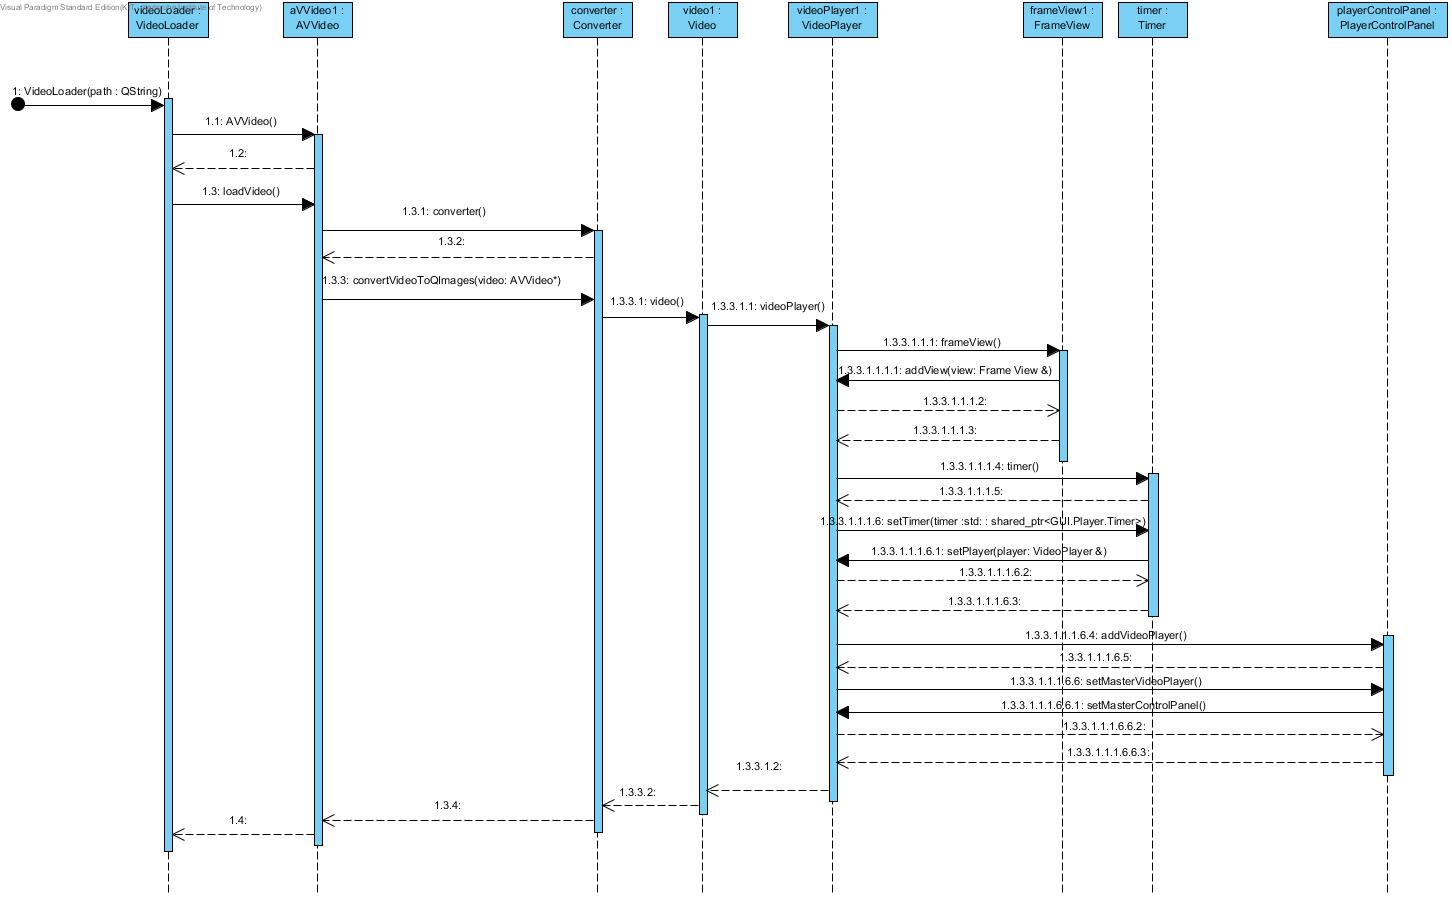
\includegraphics[width=10cm]{Sequence Diagram1.jpg}}\\
When you load a new Video a LoadVideo object is created with the path to the Video as a parameter.Then a AVVideo is created and with the Converter a Video which is then given to a VideoPlayer. This VideoPlayer has a FrameView a Timer and is then given to a ControlPanel
\newpage
{\centering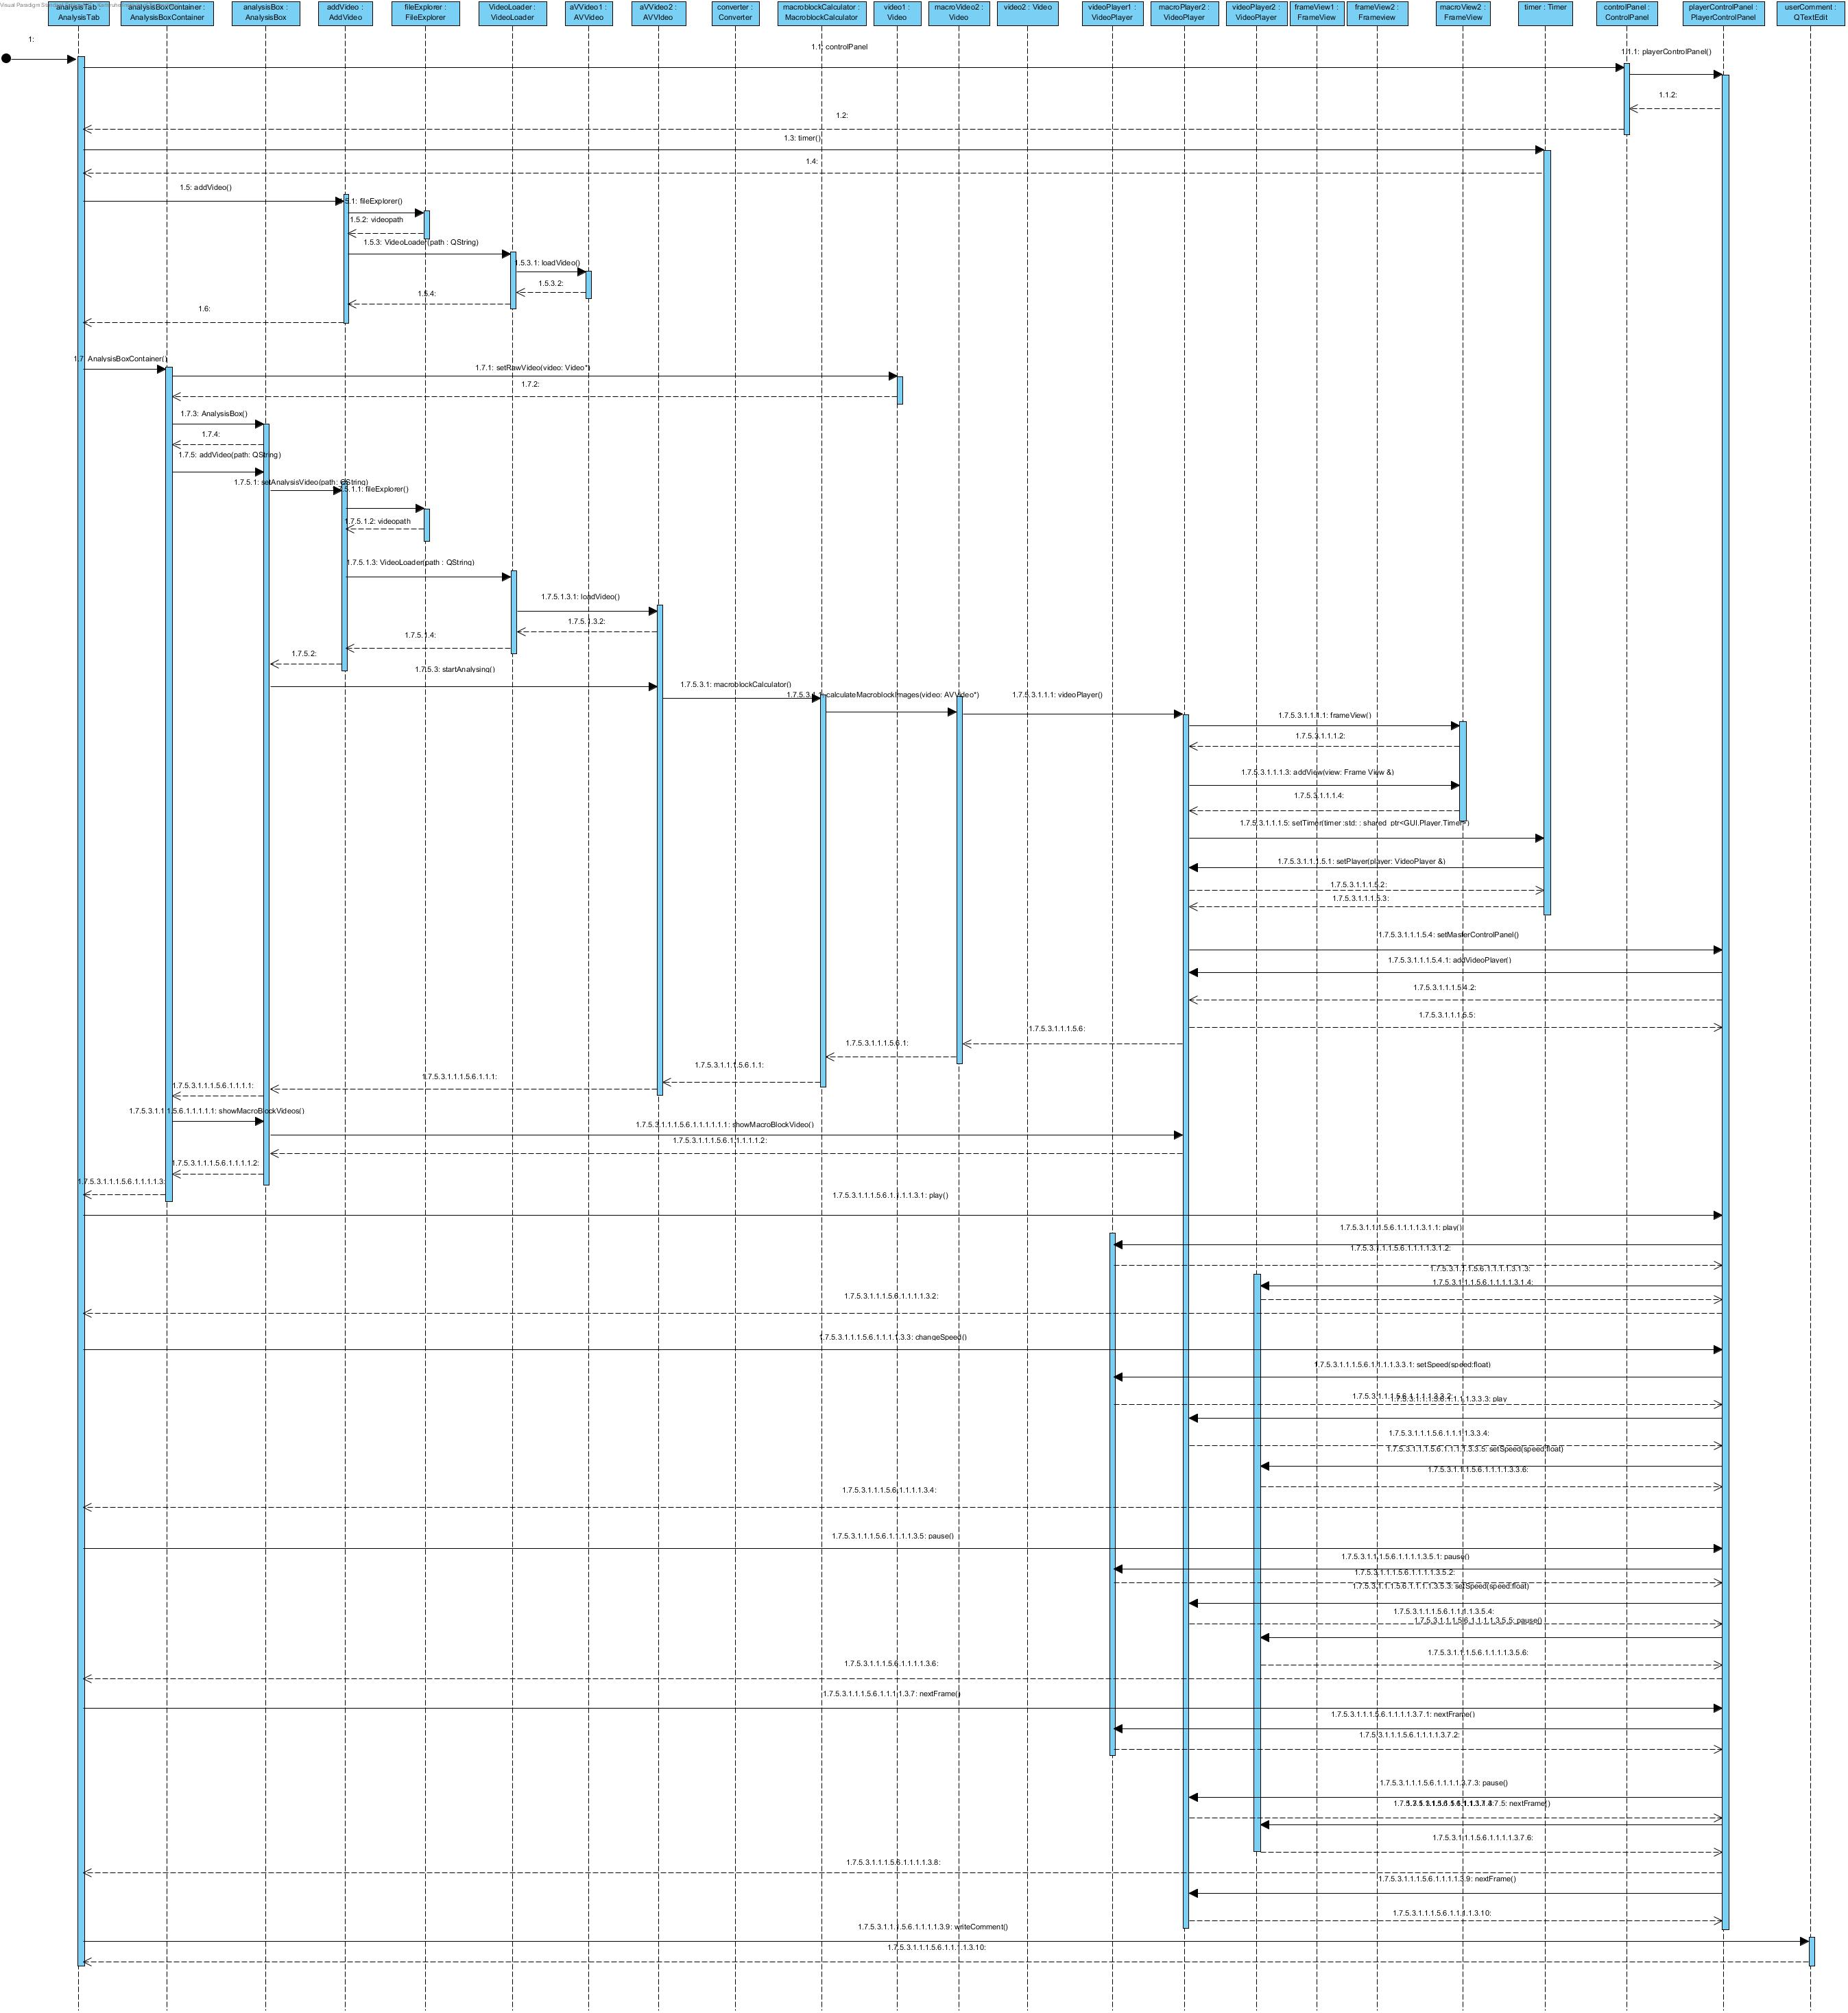
\includegraphics[width=10cm]{Sequence Diagram2.jpg}}\\
First a ControlPanel and a PlayerControlPanel are created. When a Video is added the LoadVideo Sequenz which is descriped above is initiated.  If an additional Video is added  
an AnalysisBox is created in which the added Video is loaded and the Analysis starts in which he MacroblocVideo is calculated and Displayed in a second VideoPlayer.
When play is pressed in the ControlPanel all Videos start to play.
\newpage
{\centering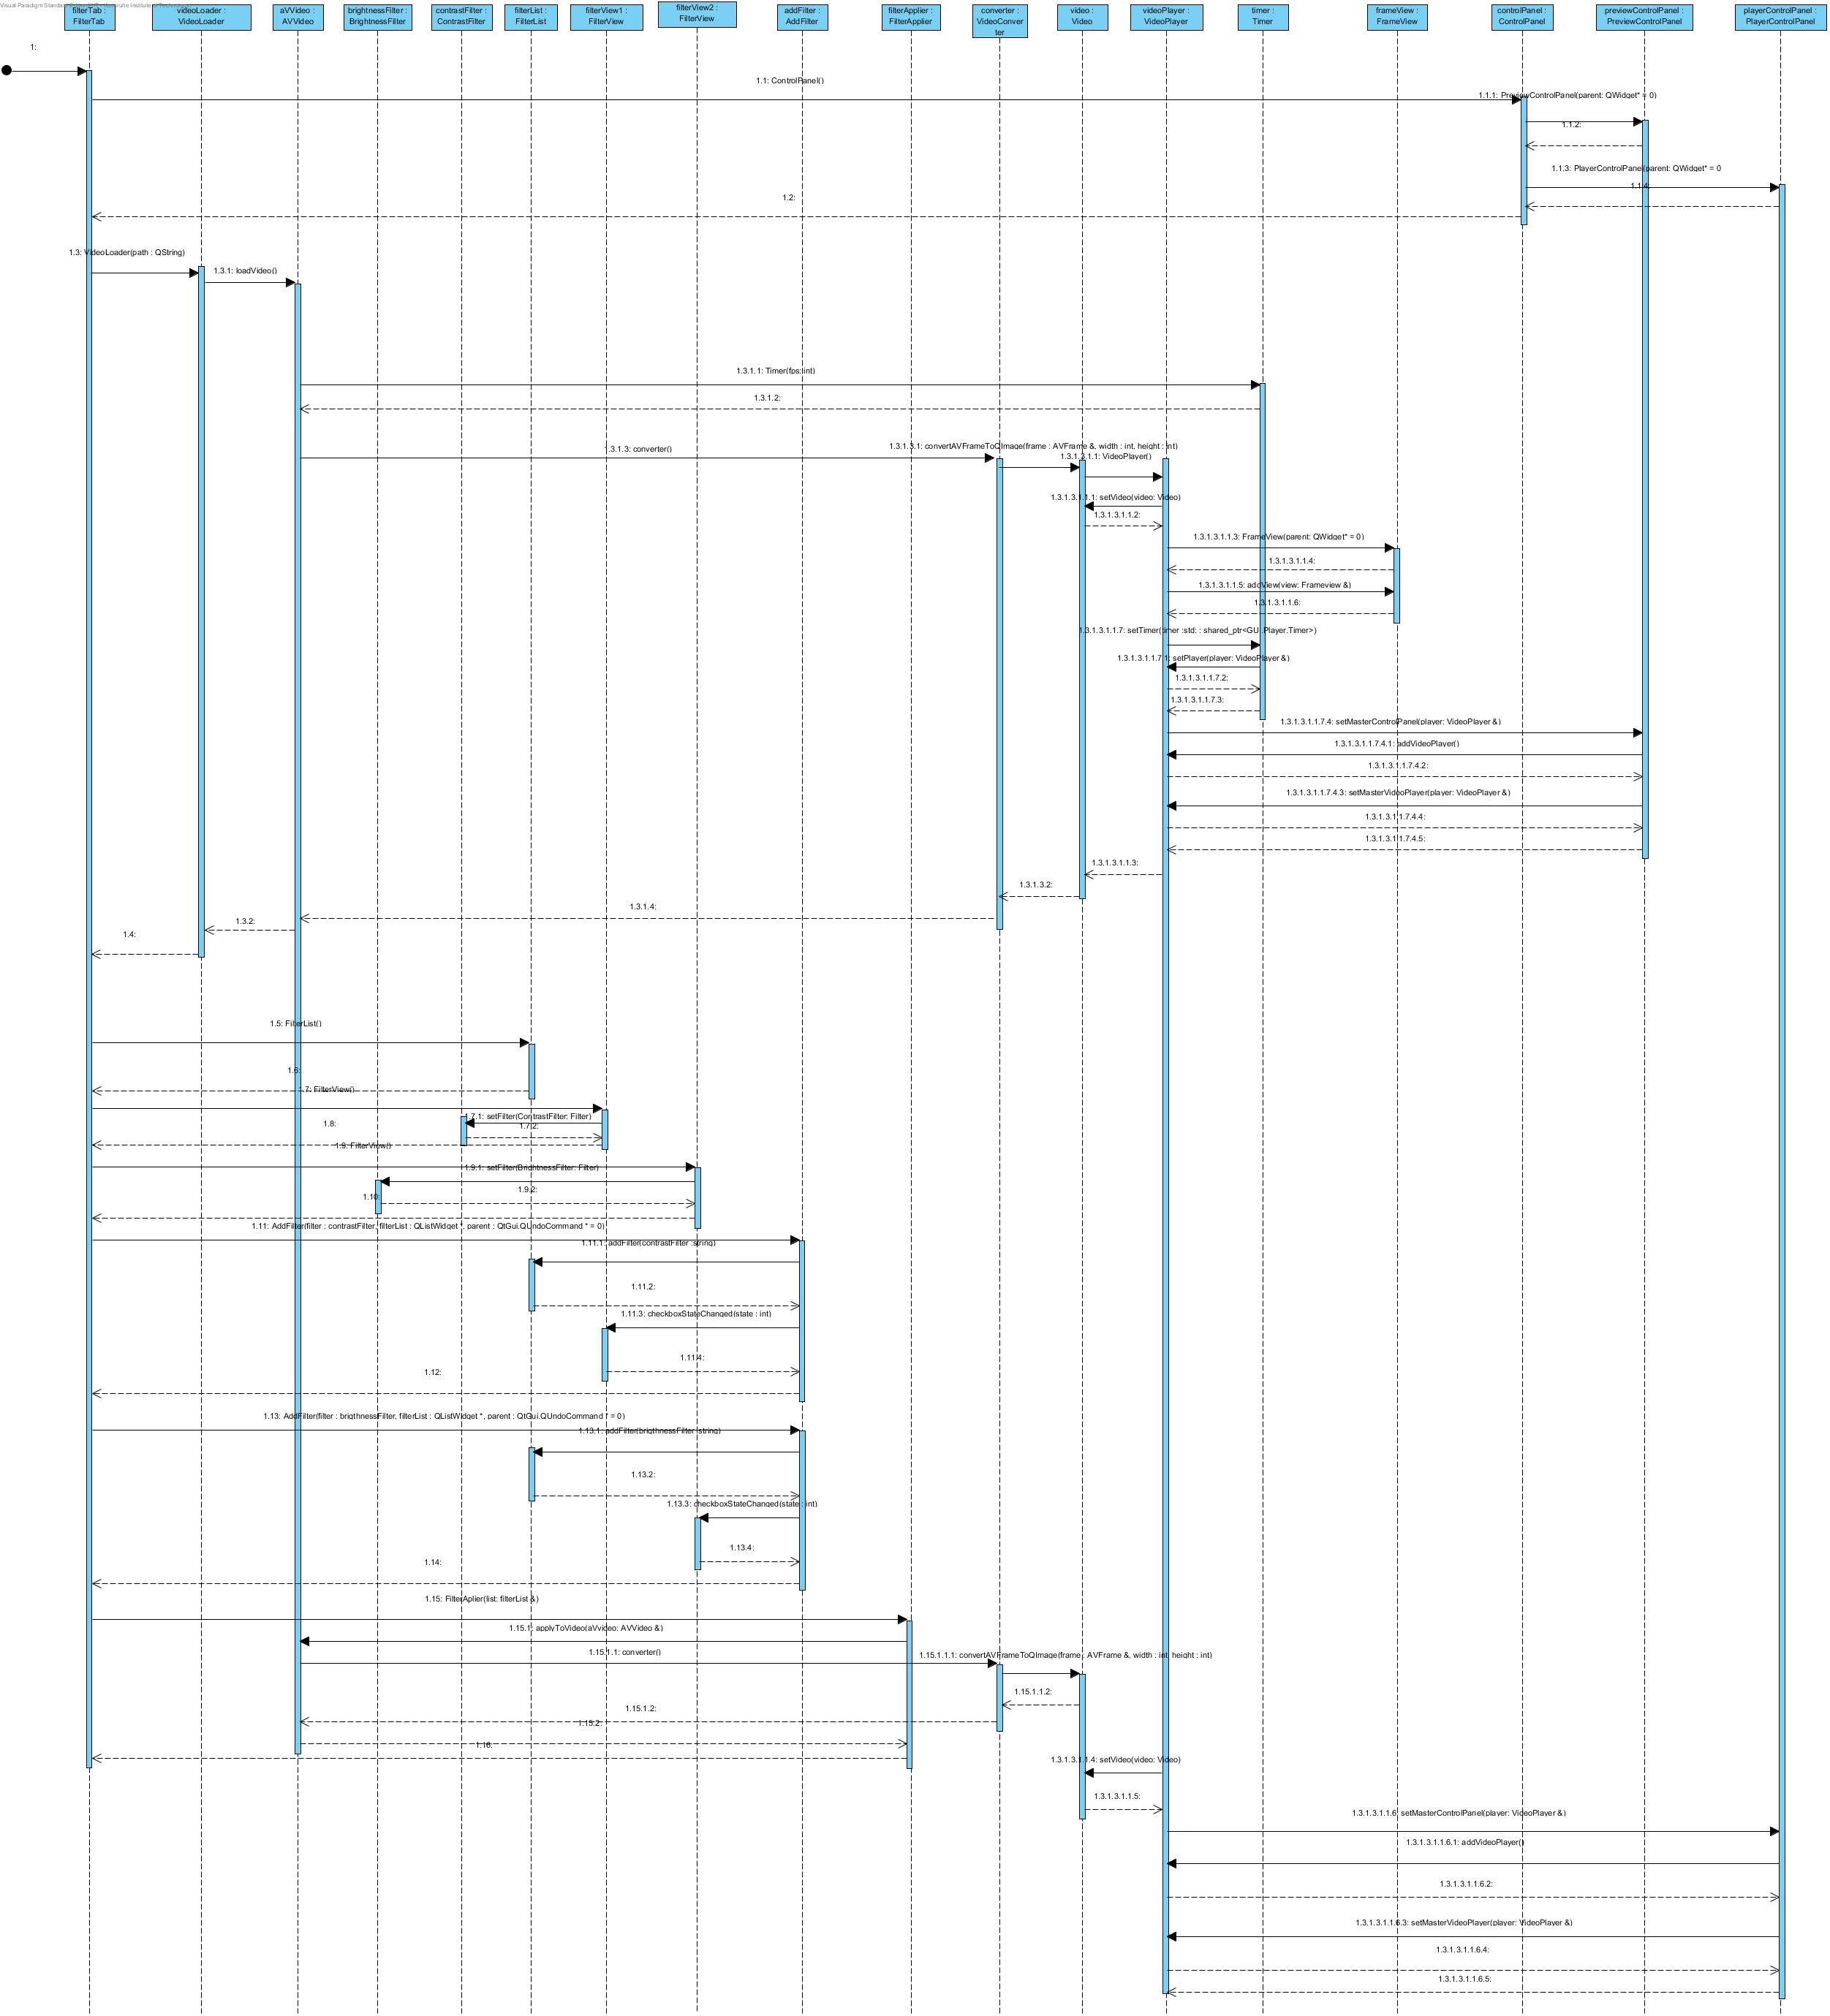
\includegraphics[width=10cm]{Sequence Diagram3.jpg}}\\
First the ControlPanel, PlayerControlPanel and PreviewControlPanel are created.
Then a Video is loaded with the LoadVideo sequenz. Then a Filter are added to the FilterList. This FilterLis is then applied to the AVVideo which is the converted to an Video and Displayed in the VideoPlayer. 
\end{document}
